\chapter{Systematic Uncertainties and Cross-checks}
\label{ch:systematics}
While it would be nice to produce exact results for the measurements presented in this thesis, uncertainties are inevitable. These uncertainties are usually grouped into two categories: \textbf{statistical uncertainties} and \textbf{systematic uncertainties}. Statistical uncertainties are those which arise from things like detector imprecision or even the inherent statistical nature of the measurement itself. Calculating these uncertainties is usually straightforward, though it often involves well-motivated assumptions about the underlying probability distributions of the data. Determining systematic uncertainties, on the other hand, is a much more complicated process. To that end, the first section of this chapter goes into a large amount of detail about the calculation of systematic uncertainties for this analysis, starting with clearly defining what ``systematic uncertainty'' means and how it is quantified in the context of this thesis, followed by comprehensive investigations into each of the sources of uncertainty considered in this research, and ending with a summary of the final systematic uncertainties for each observable.

The second section of this chapter is dedicated to the cross-checks performed to ensure the validity of the analysis procedure. There are a variety of such checks, ranging from a general Monte Carlo closure test to more specific checks into physical biases that may be introduced by the analysis procedure.


\clearpage

\section{Systematic uncertainties}
\label{sec:systematics}
\begin{quote}
    \textit{``The treatment of systematic errors is often mishandled. This is due to lack of understanding and education, based on a fundamental ambiguity as to what is meant by the term''}\\
    \hspace*{1cm}---Roger Barlow, \textit{Systematic Errors: Facts and Fictions}~\cite{BarlowCheck}
\end{quote}

In every experimental analysis, choices must be made. These choices can be as simple as the selection of a particular data set, or as complex as choosing a fit function of fifteen parameters instead of three. In either case, these choices can have an effect on the final results, which is usually quantified by the \textbf{systematic uncertainty}. Broadly speaking, the systematic uncertainty is a measure of the sensitivity of the final results to the choices made during the analysis procedure. 

In this analysis, the procedure for estimating the systematic uncertainty from a certain choice is as follows:
%
\begin{enumerate}
    \item Vary the choice in a way that is reasonable and justifiable 
    \item Measure the observable of interest after the variation
    \item Quantify the effect of the variation on the observable by calculating the percent change from the original value of the observable
    \item Vary the choice in a slightly different way, and repeat steps 2 and 3
    \item Repeat steps 2 through 4 until all reasonable variations have been considered
    \item Calculate the systematic uncertainty as the root mean square (RMS) of the percentages from step 3.
\end{enumerate}
%
Note the usage of the words ``reasonable'' and ``justifiable'', which seem to indicate that the systematic uncertainty is a subjective quantity. Indeed, the process of obtaining the systematic uncertainty involves even more choices, like the choice of which choices to consider, the choices of how to vary the choices, and even the choice on how to quantify the uncertainty itself. In this sense, systematic uncertainty calculations are an art form, where the artist (analyzer) must use their creativity and best judgement to determine which choices are indeed reasonable. To that end, the list of sources of systematic uncertainties considered for this analysis is not exhaustive, but it is the best attempt at a comprehensive list of reasonable choices that affect the final results. 

To provide more structure to this section, the analysis procedure is broken into the following components:
%
\begin{enumerate}
\item The generation of the h-$\Lambda$ and h-h $\Delta\varphi$ distributions,
\item The extraction of the pairwise yields from the $\Delta\varphi$ distributions, and 
\item The extraction of the near- and away-side widths from the fits of the $\Delta\varphi$ distributions,
\end{enumerate}
%
which are used to separate this section into three subsections, one for each of these components. In each section, the sources of systematic uncertainties are described, followed by a Barlow analysis~\cite{BarlowCheck} to ensure the variations result in a statistically significant deviation from the nominal values. Finally, a summary of the final systematic uncertainties is provided.

\subsection{$\Delta\varphi$ distribution generation}
\label{sec:systematics_dphi}
The sources of systematic uncertainties that affect the $\Delta\varphi$ distribution considered for this analysis are the following, in order of decreasing magnitude:
%
\begin{itemize}
\item \lmb topological selection (h-\lmb distribution only)
\item Material budget
\item Tracking efficiency
\item \lmb daughter PID cuts (h-\lmb distribution only)
\item \lmb invariant mass signal region selection (h-\lmb distribution only)
\item \lmb invariant mass sideband region selection (h-\lmb distribution only)
\end{itemize}
%
As the \lmb topological selection, material budget, and tracking efficiencies have been studied in detail in previous analyses using the same particle species and collision system
~\cite{V0Reco1,V0Reco1,Lambda1,ALICEMatBud}, the systematic uncertainty associated with these sources is taken directly from these analyses and presented in Table~\ref{tab:flat_systematics}. The uncertainties from these sources exhibit no multiplicity dependence, and a very small dependence on \pt. These uncertainties are also assumed to be independent of $\Delta\varphi$, although this is studied more thoroughly in Section~\ref{sec:systematics_width}.

Each of the other sources of systematic uncertainty is described in detail in the following sections. 

\begin{table}
    \centering
    \caption{The systematic uncertainties for the $\Delta\varphi$ distributions which are not directly calculated in this thesis, instead taken from previous analyses using the same particle species and collision system~\cite{V0Reco1,V0Reco2,Lambda1,ALICEMatBud}. Each source of uncertainty is verified to be independent of multiplicity, but the \lmb material budget and topological selection uncertainties exhibit a small dependence on \pt. }
    \label{tab:flat_systematics}
    \begin{tabular}{l c c}
        \hline
        Source name & Lower \pt \% & Higher \pt \% \\
        \hline
        \lmb topological selection & 3.2\% & 3.0\% \\
        \lmb material budget & 1.1\% & 0.6\% \\
        Charged h tracking efficiency & 3.5\% & 3.5\% \\
        Charged h material budget & negl. & negl. \\
        \hline
    \end{tabular}
\end{table}

\subsubsection{Signal region selection}
The nominal signal region for the \lmb invariant mass is fairly wide, accounting for nearly 97\% of the total \lmb signal.  However, the final result should not be heavily influenced by the choice of signal region so long as it is centered about the true \lmb mass. Furthermore, altering the signal region tests the validity of the signal scaling procedure outlined in Section~\ref{sec:corrections}. To investigate this, the signal region is varied in the ways presented in Table~\ref{tab:signal_region_variations}. The resulting $\Delta\varphi$ distributions and ratios to the nominal distribution for each signal region variation in each multiplicity and associated \pt bin are shown in Figures \ref{fig:signal_region_variations_lowpt} (lower \pt) and \ref{fig:signal_region_variations_highpt} (higher \pt). The average deviation from the nominal distribution is around 2\%, with no individual variation exceeding 5\%. As no significant dependence on $\Delta\varphi$ is observed, the systematic uncertainty is calculated as the RMS of the percent change from each variation across the entire $\Delta\varphi$ range as opposed to calculating the RMS in each bin.

\begin{table}[ht]
    \centering
    \caption{The variations of the \lmb invariant mass signal region considered for this analysis.}
    \label{tab:signal_region_variations}
    \begin{tabular}{l c}
        \hline
        Variation name & Signal range (GeV/$c^2$) \\
        \hline
        Narrow & $1.108 < M_{p\pi} < 1.124$ \\
        Narrower & $1.112 < M_{p\pi} < 1.120$ \\
        Wide & $1.100 < M_{p\pi} < 1.132$ \\
        Wider & $1.096 < M_{p\pi} < 1.136$ \\
        \hline
    \end{tabular}
\end{table}

\begin{figure}[ht]
    \centering
    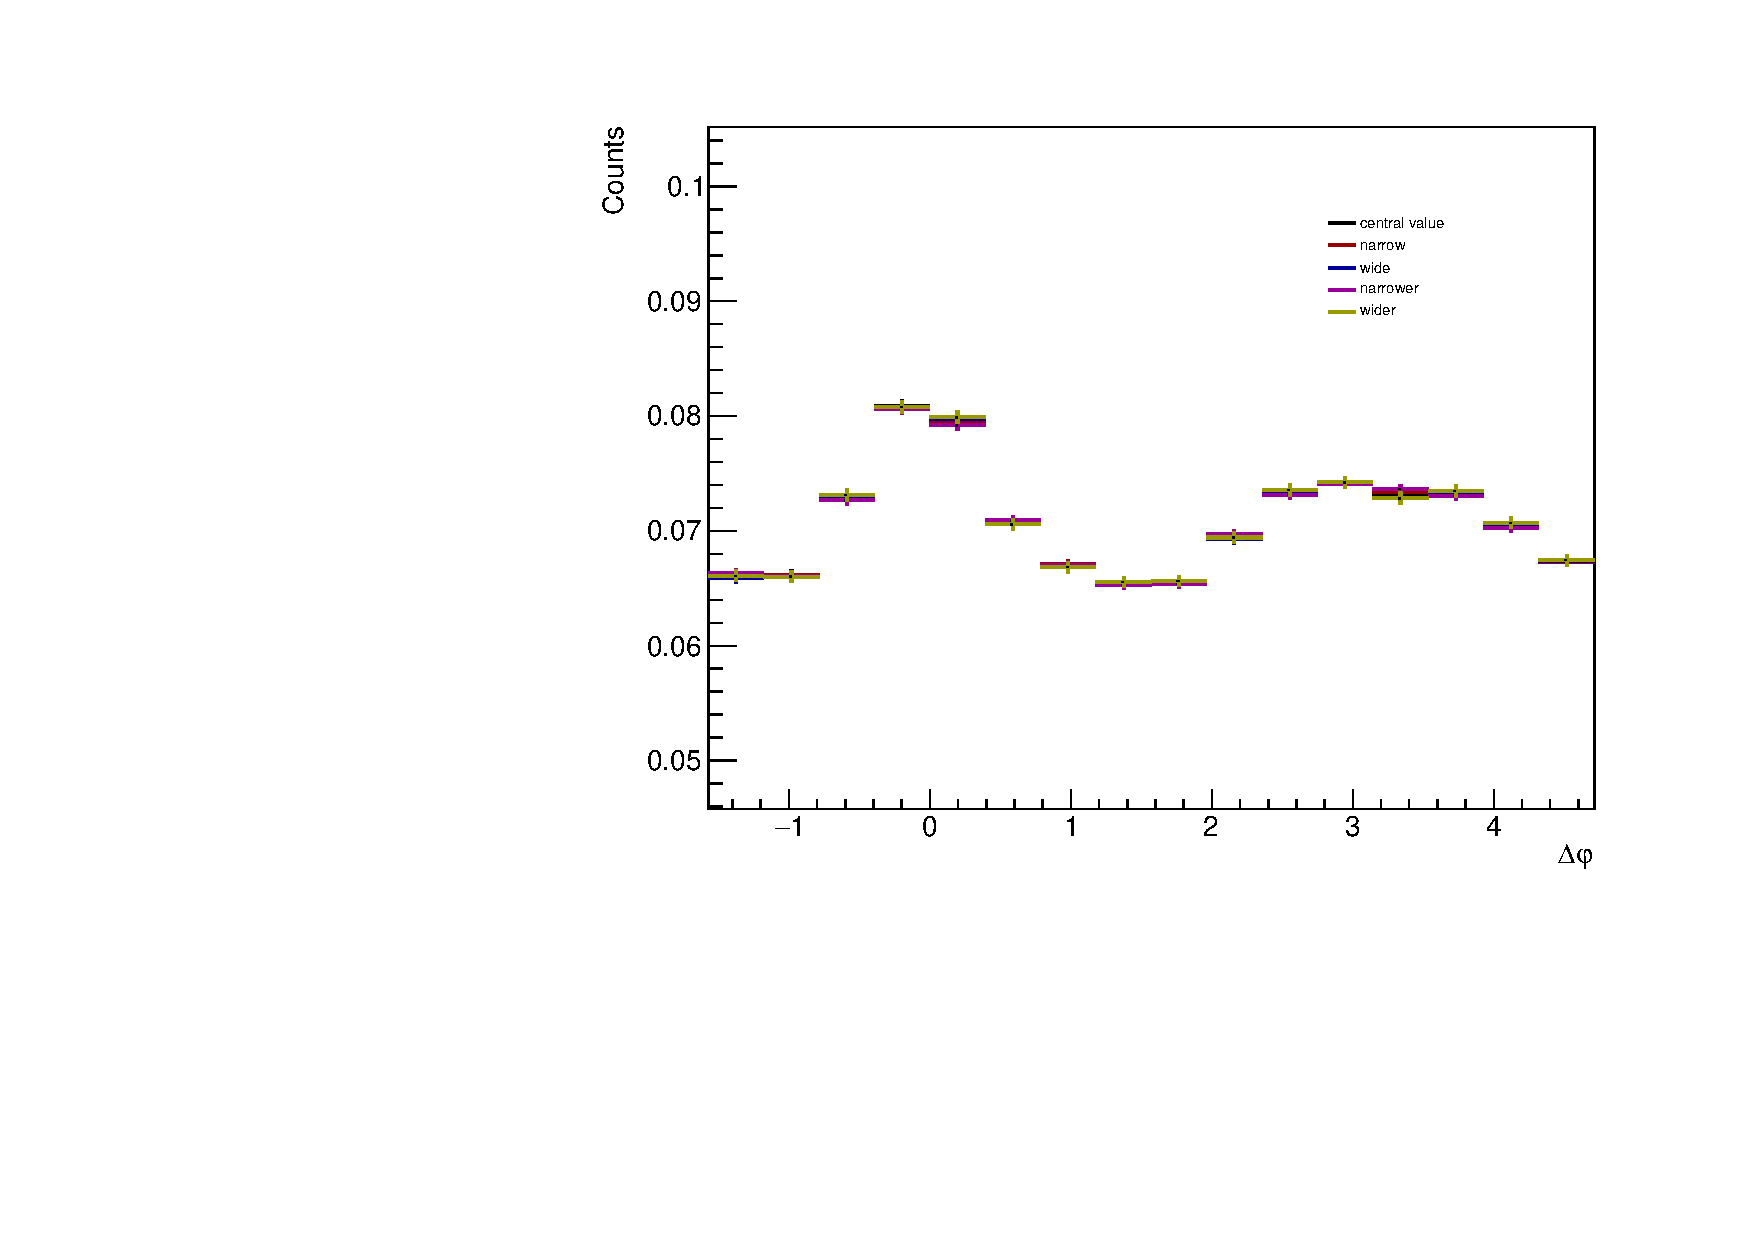
\includegraphics[width=0.49\textwidth]{figures/analysis/signal_variations_dphi_0_20_lowpt.pdf}
    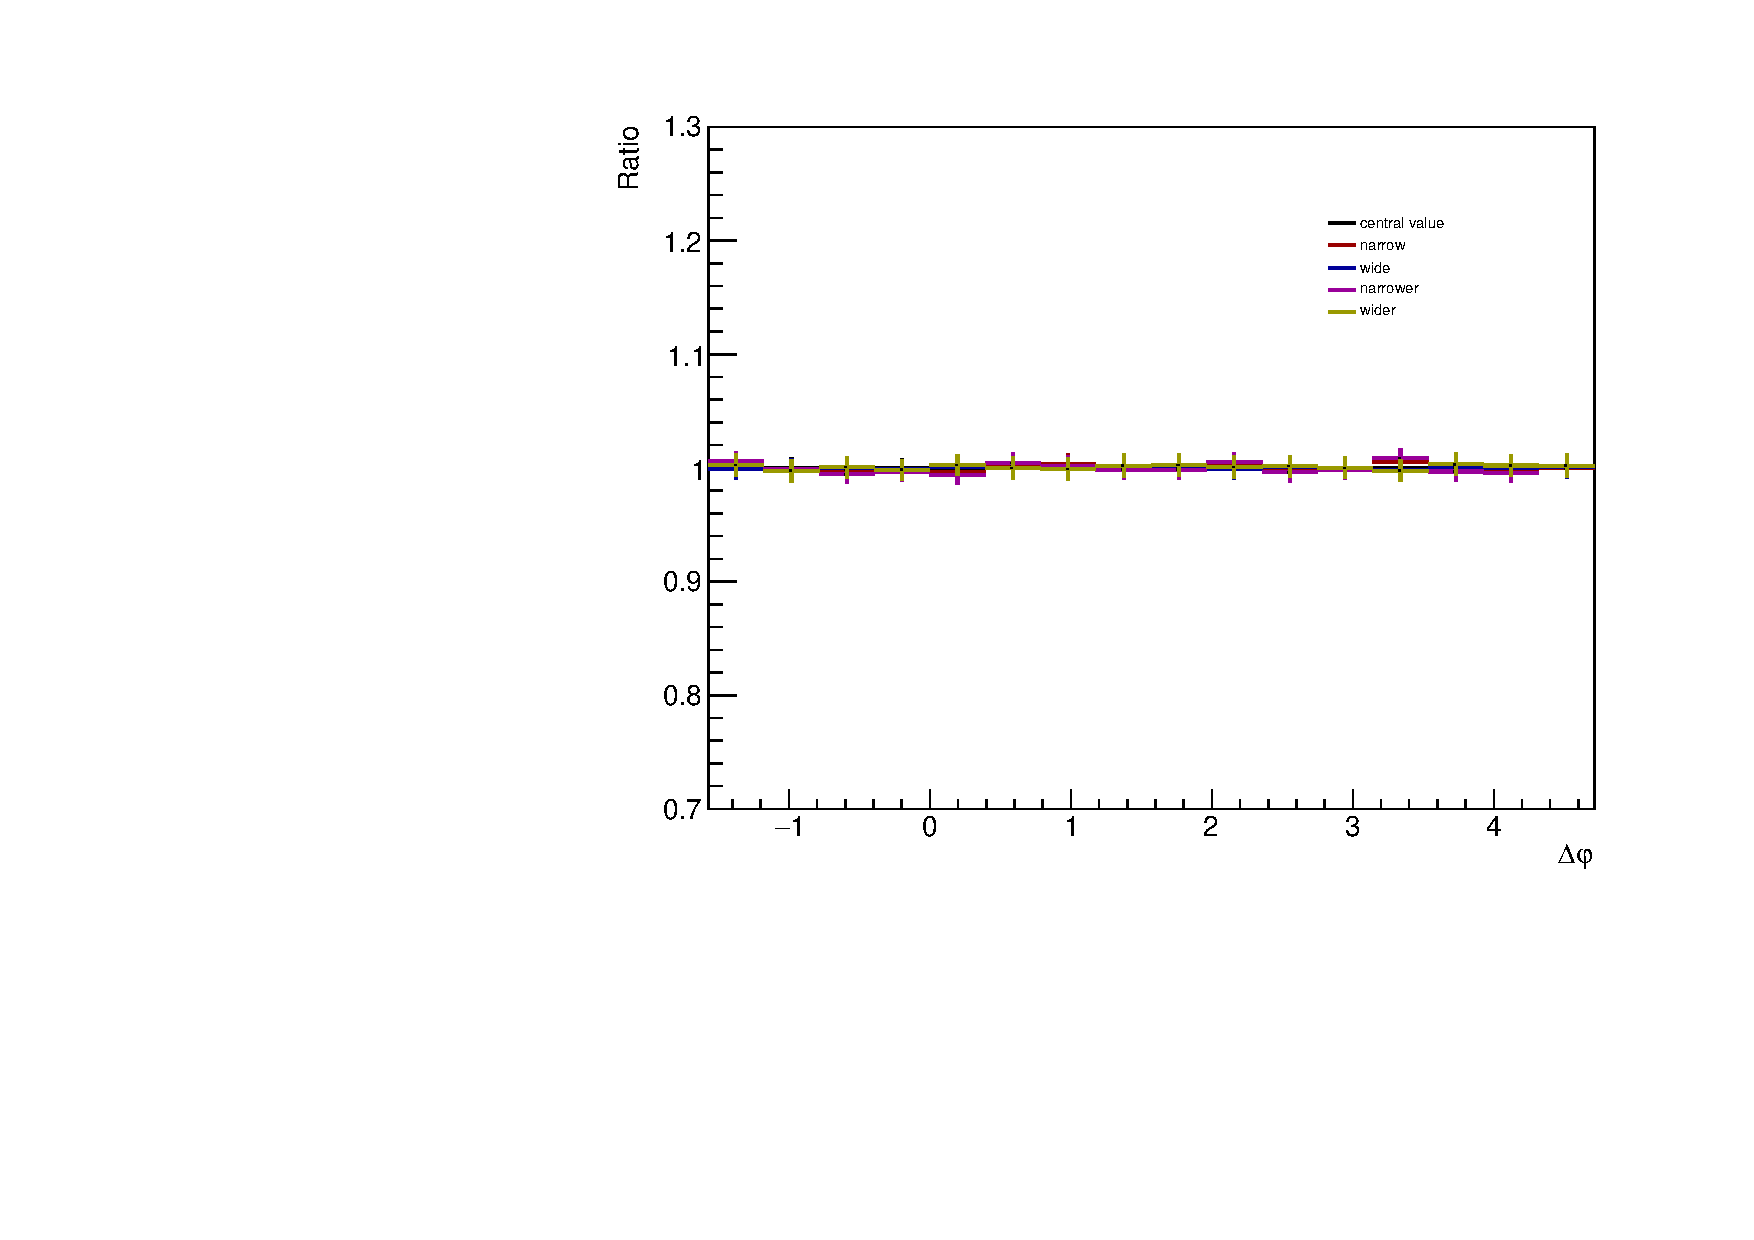
\includegraphics[width=0.49\textwidth]{figures/analysis/signal_variations_dphi_0_20_lowpt_ratio.pdf}
    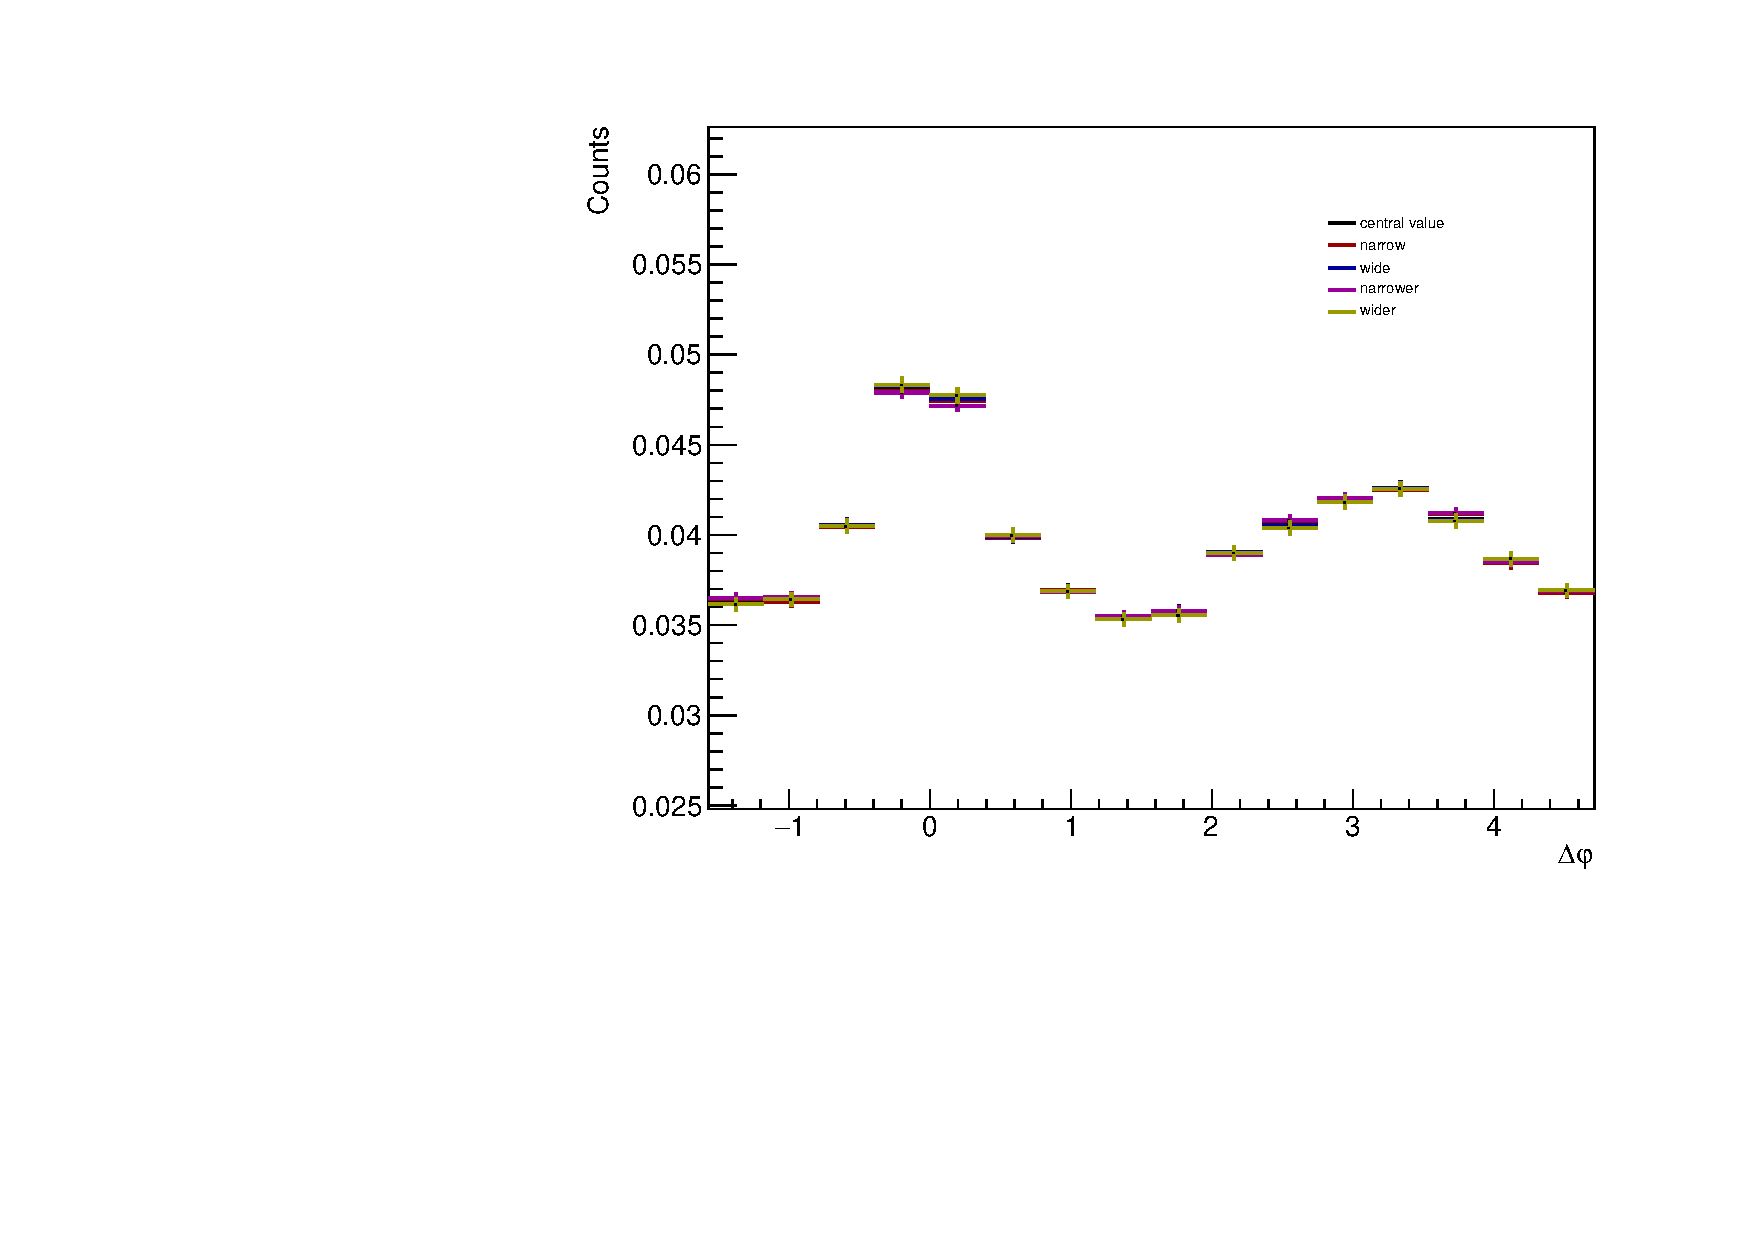
\includegraphics[width=0.49\textwidth]{figures/analysis/signal_variations_dphi_20_50_lowpt.pdf}
    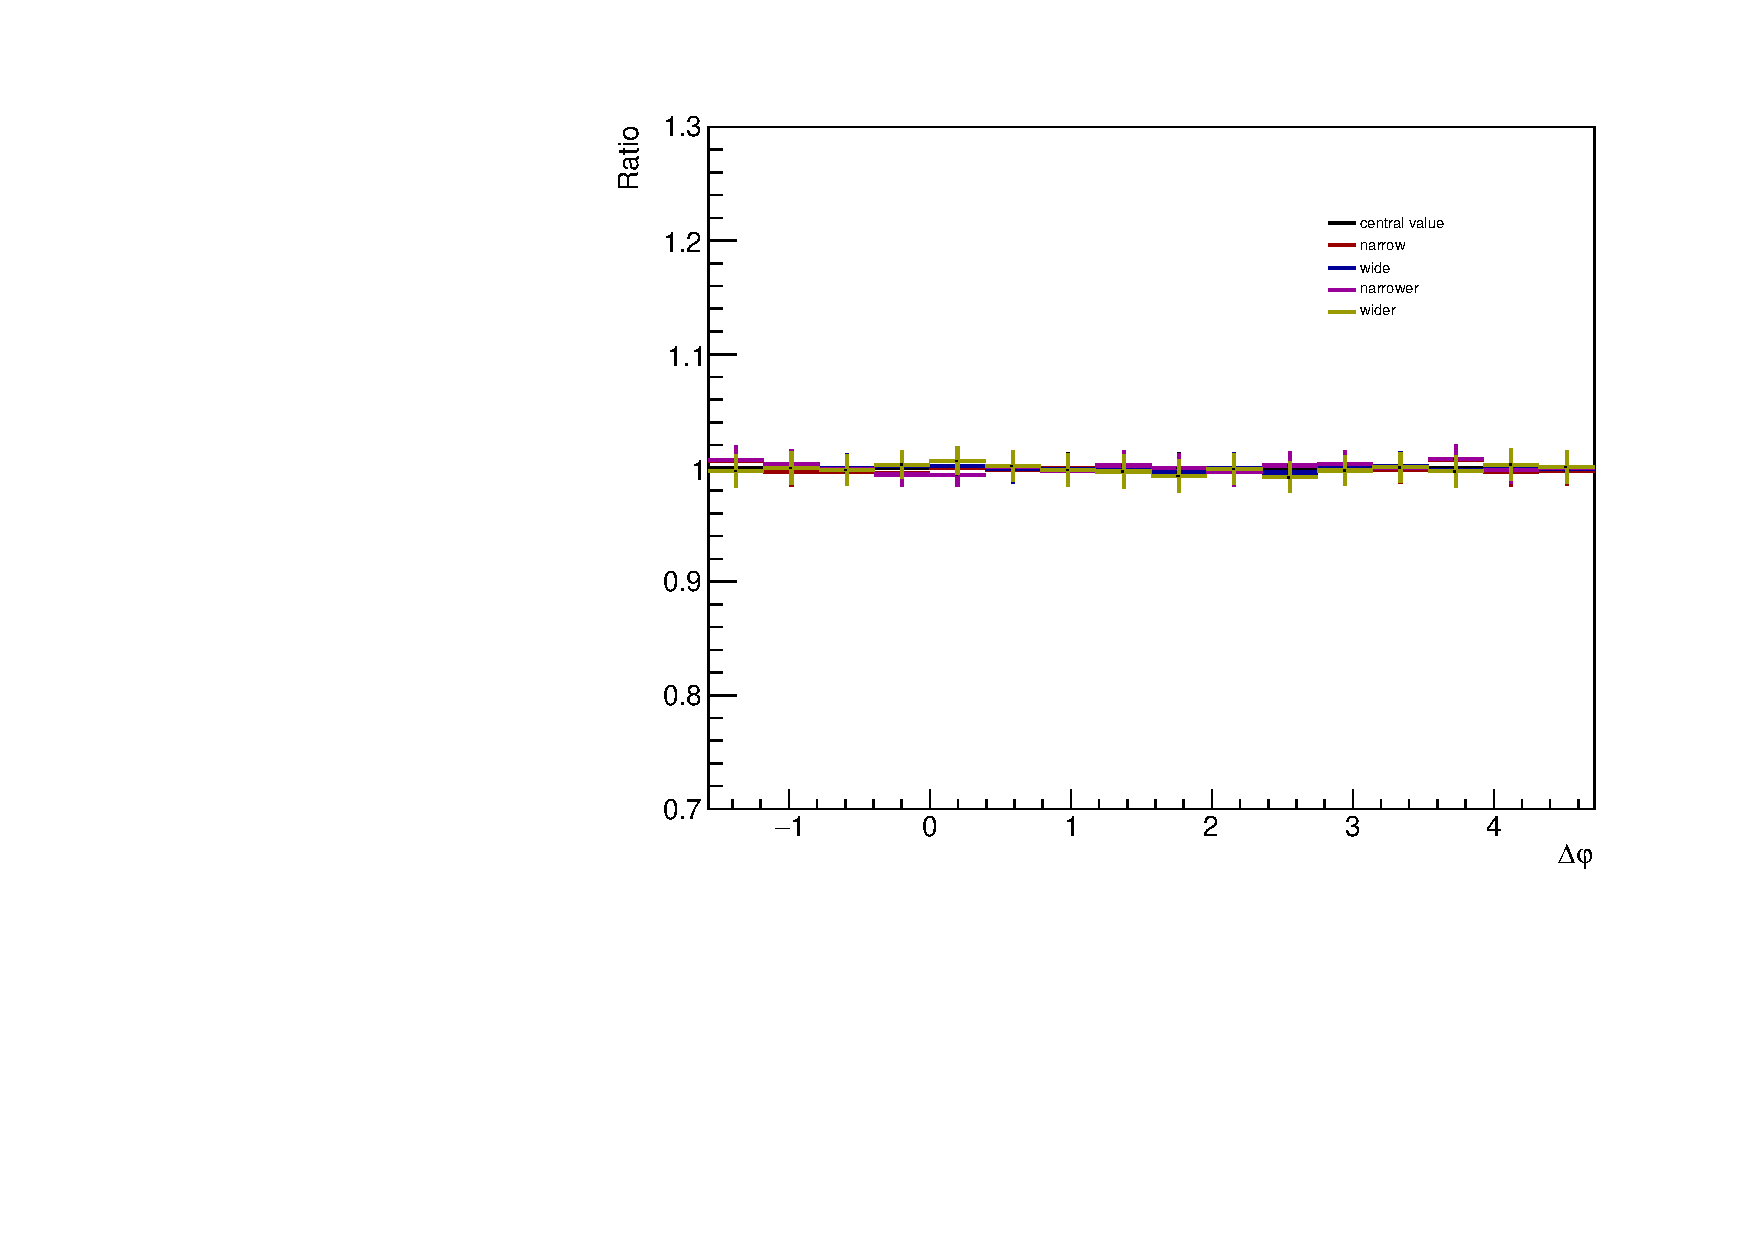
\includegraphics[width=0.49\textwidth]{figures/analysis/signal_variations_dphi_20_50_lowpt_ratio.pdf}
    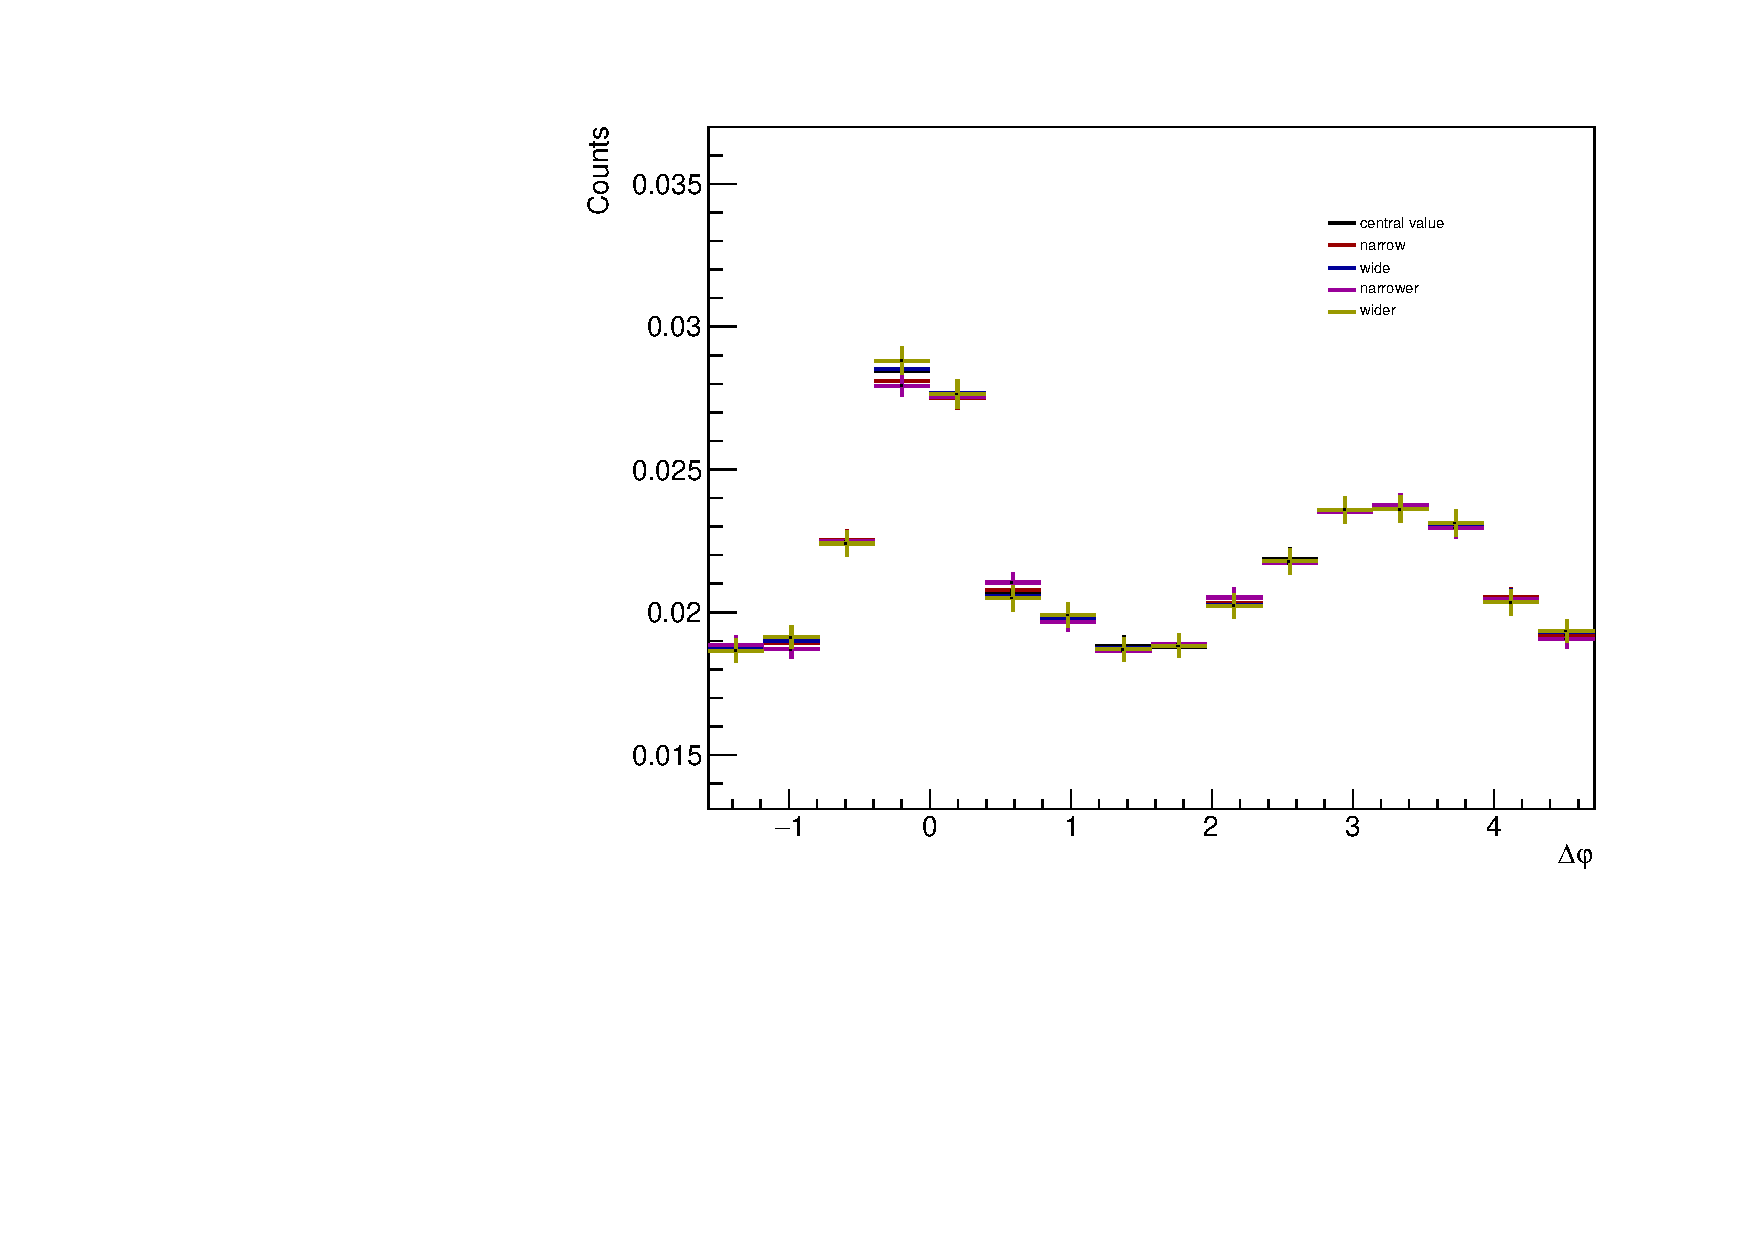
\includegraphics[width=0.49\textwidth]{figures/analysis/signal_variations_dphi_50_80_lowpt.pdf}
    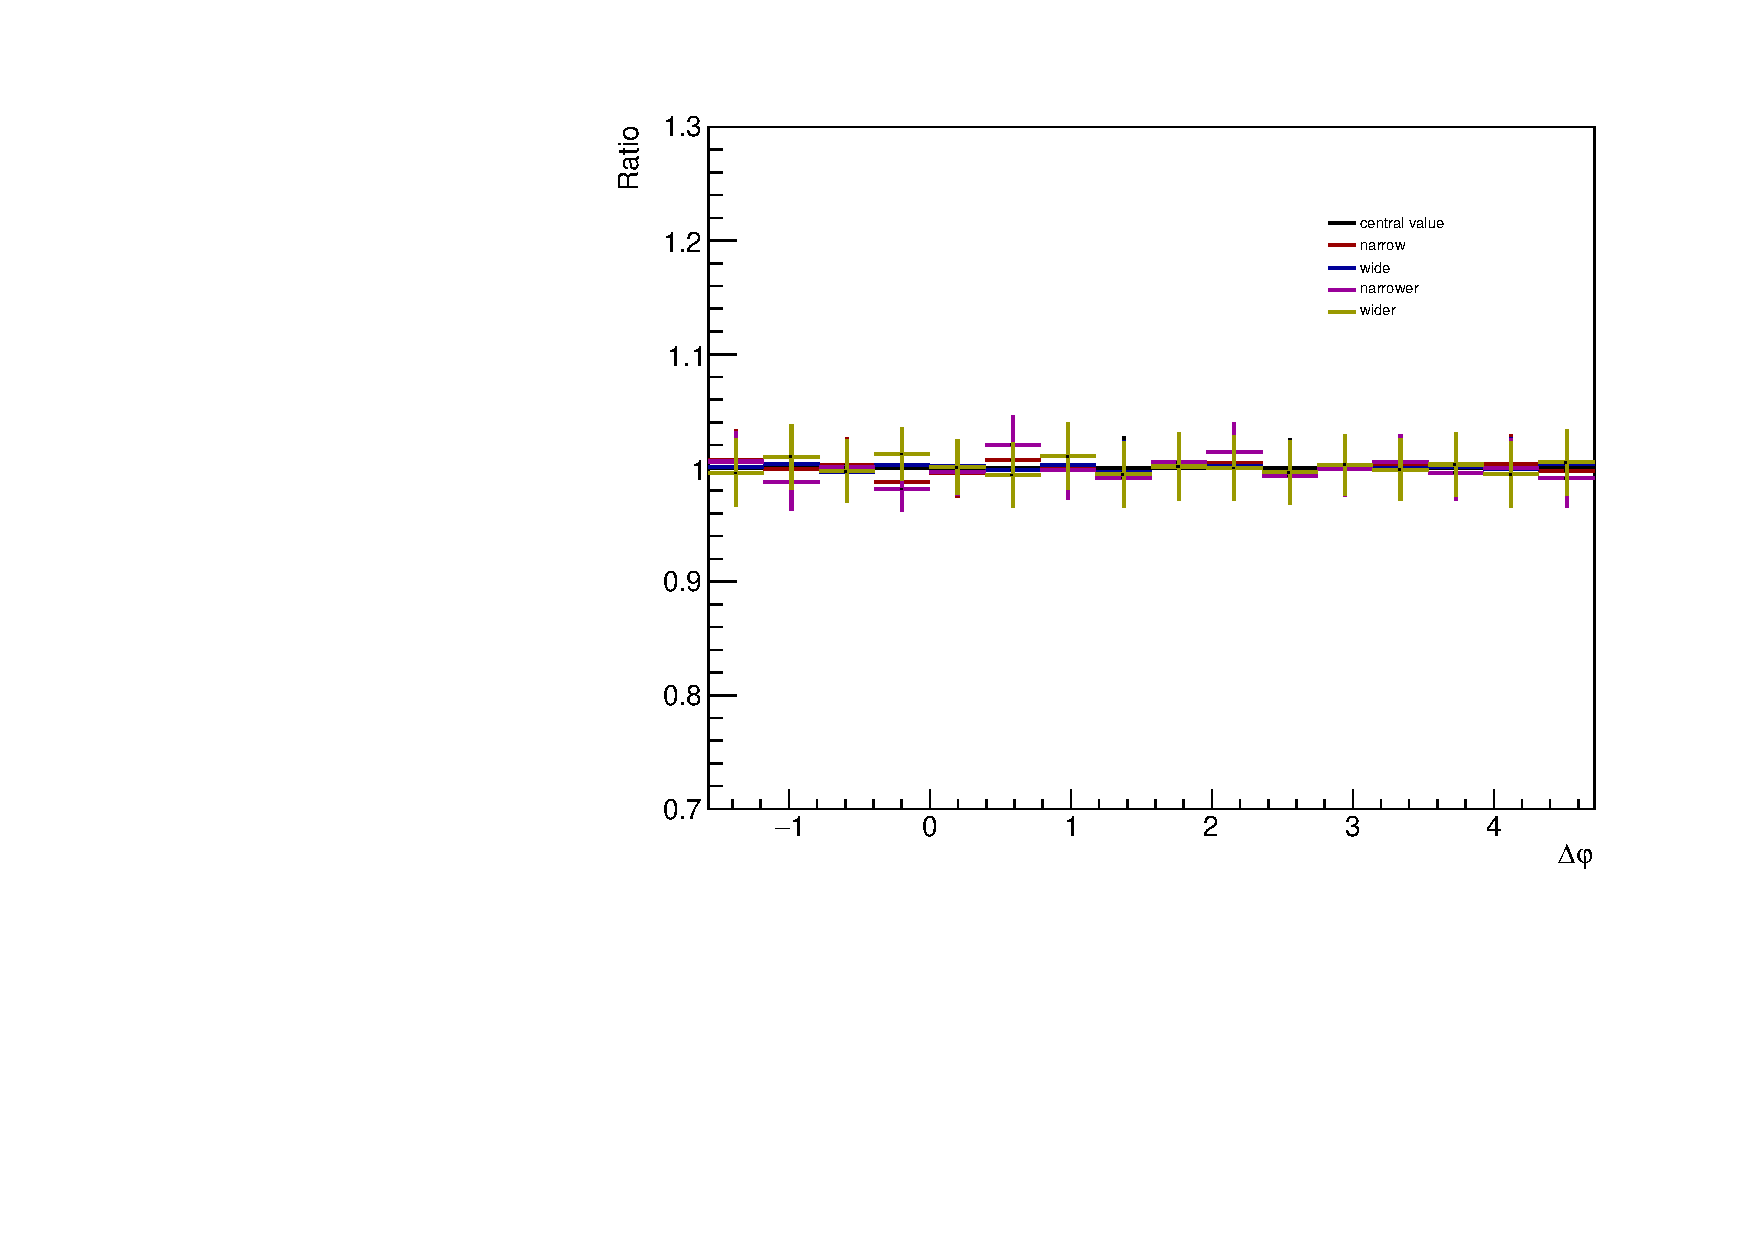
\includegraphics[width=0.49\textwidth]{figures/analysis/signal_variations_dphi_50_80_lowpt_ratio.pdf}
    \caption{The h-\lmb $\Delta\varphi$ distributions within the 0-20\% (top), 20-50\% (middle), and 50-80\% (bottom) multiplicity bins in the lower associated \pt bin for each of the signal region variations (left) with the ratios to the nominal distribution (right).}
    \label{fig:signal_region_variations_lowpt}
\end{figure}

\begin{figure}[ht]
    \centering
    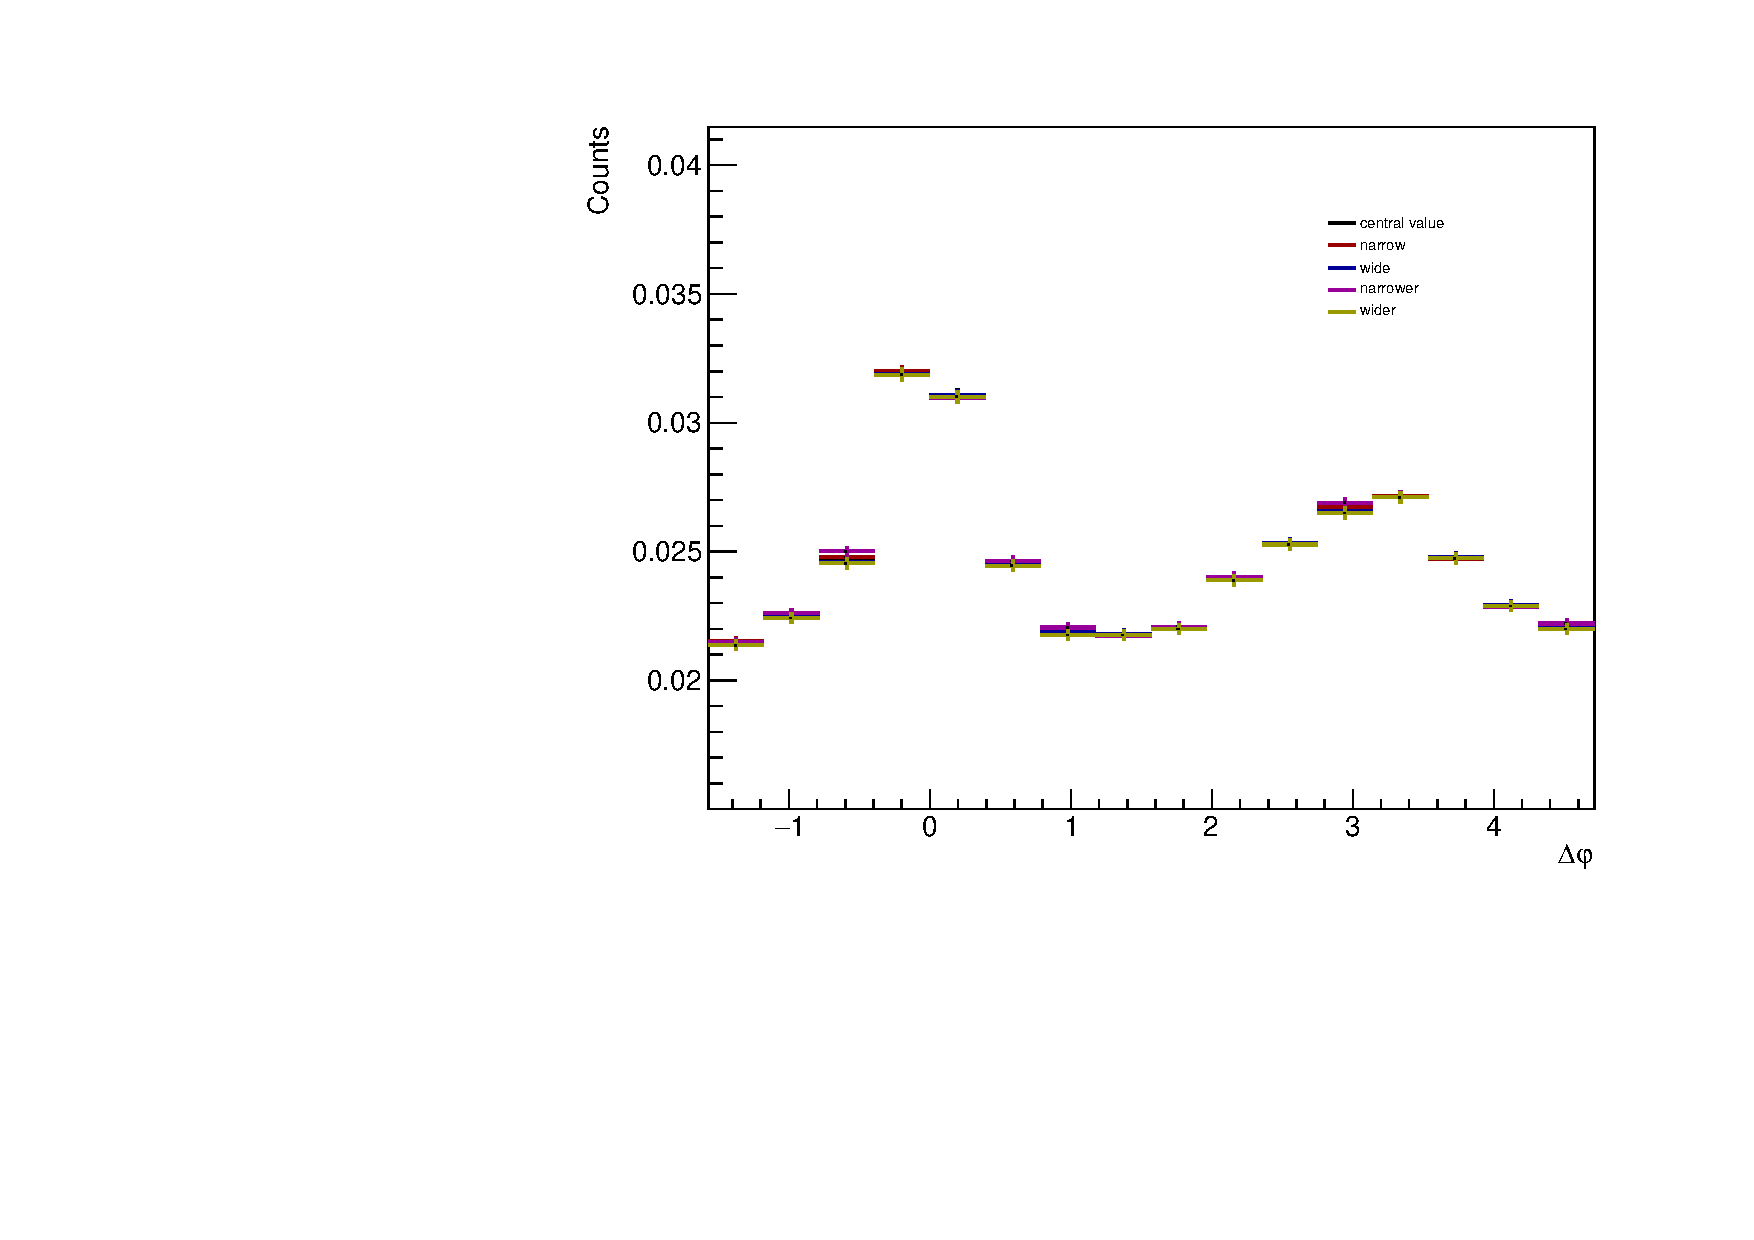
\includegraphics[width=0.49\textwidth]{figures/analysis/signal_variations_dphi_0_20_highpt.pdf}
    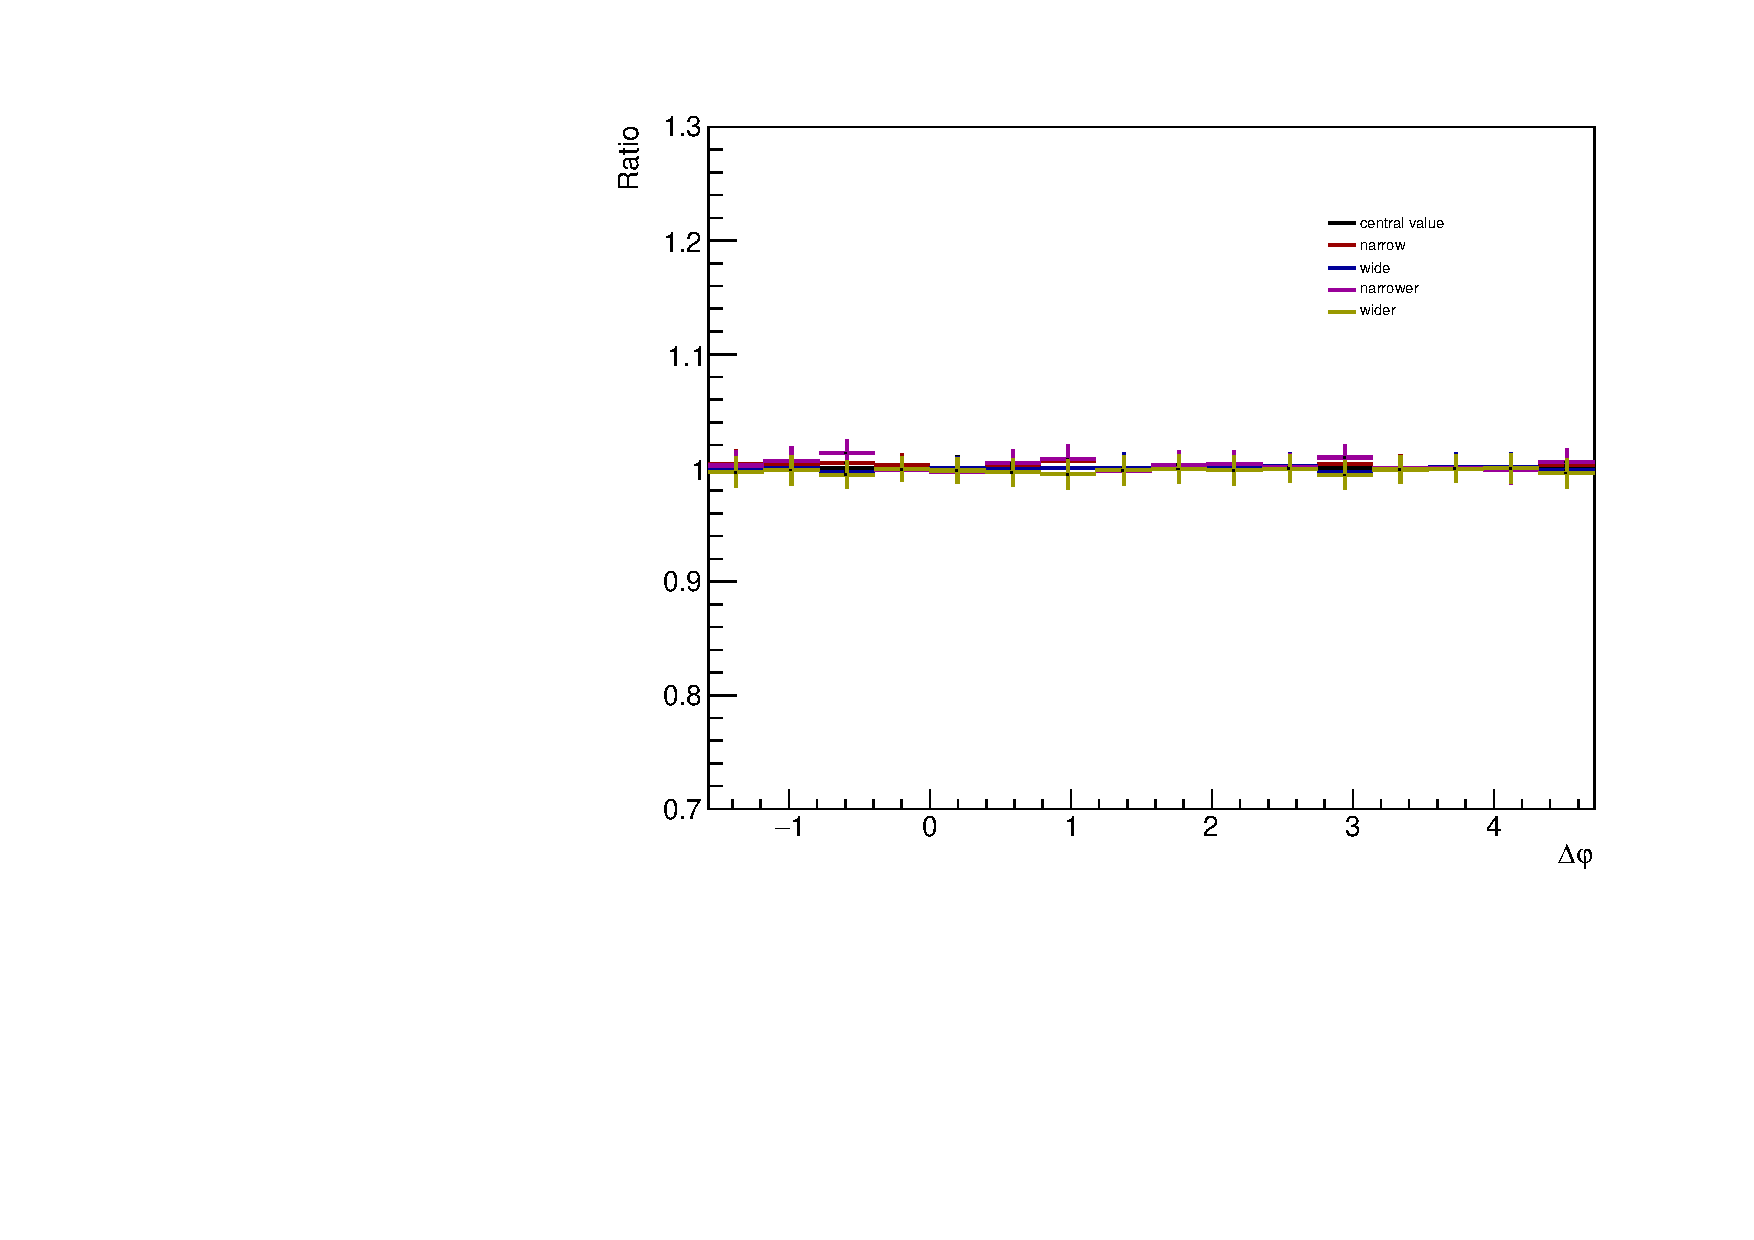
\includegraphics[width=0.49\textwidth]{figures/analysis/signal_variations_dphi_0_20_highpt_ratio.pdf}
    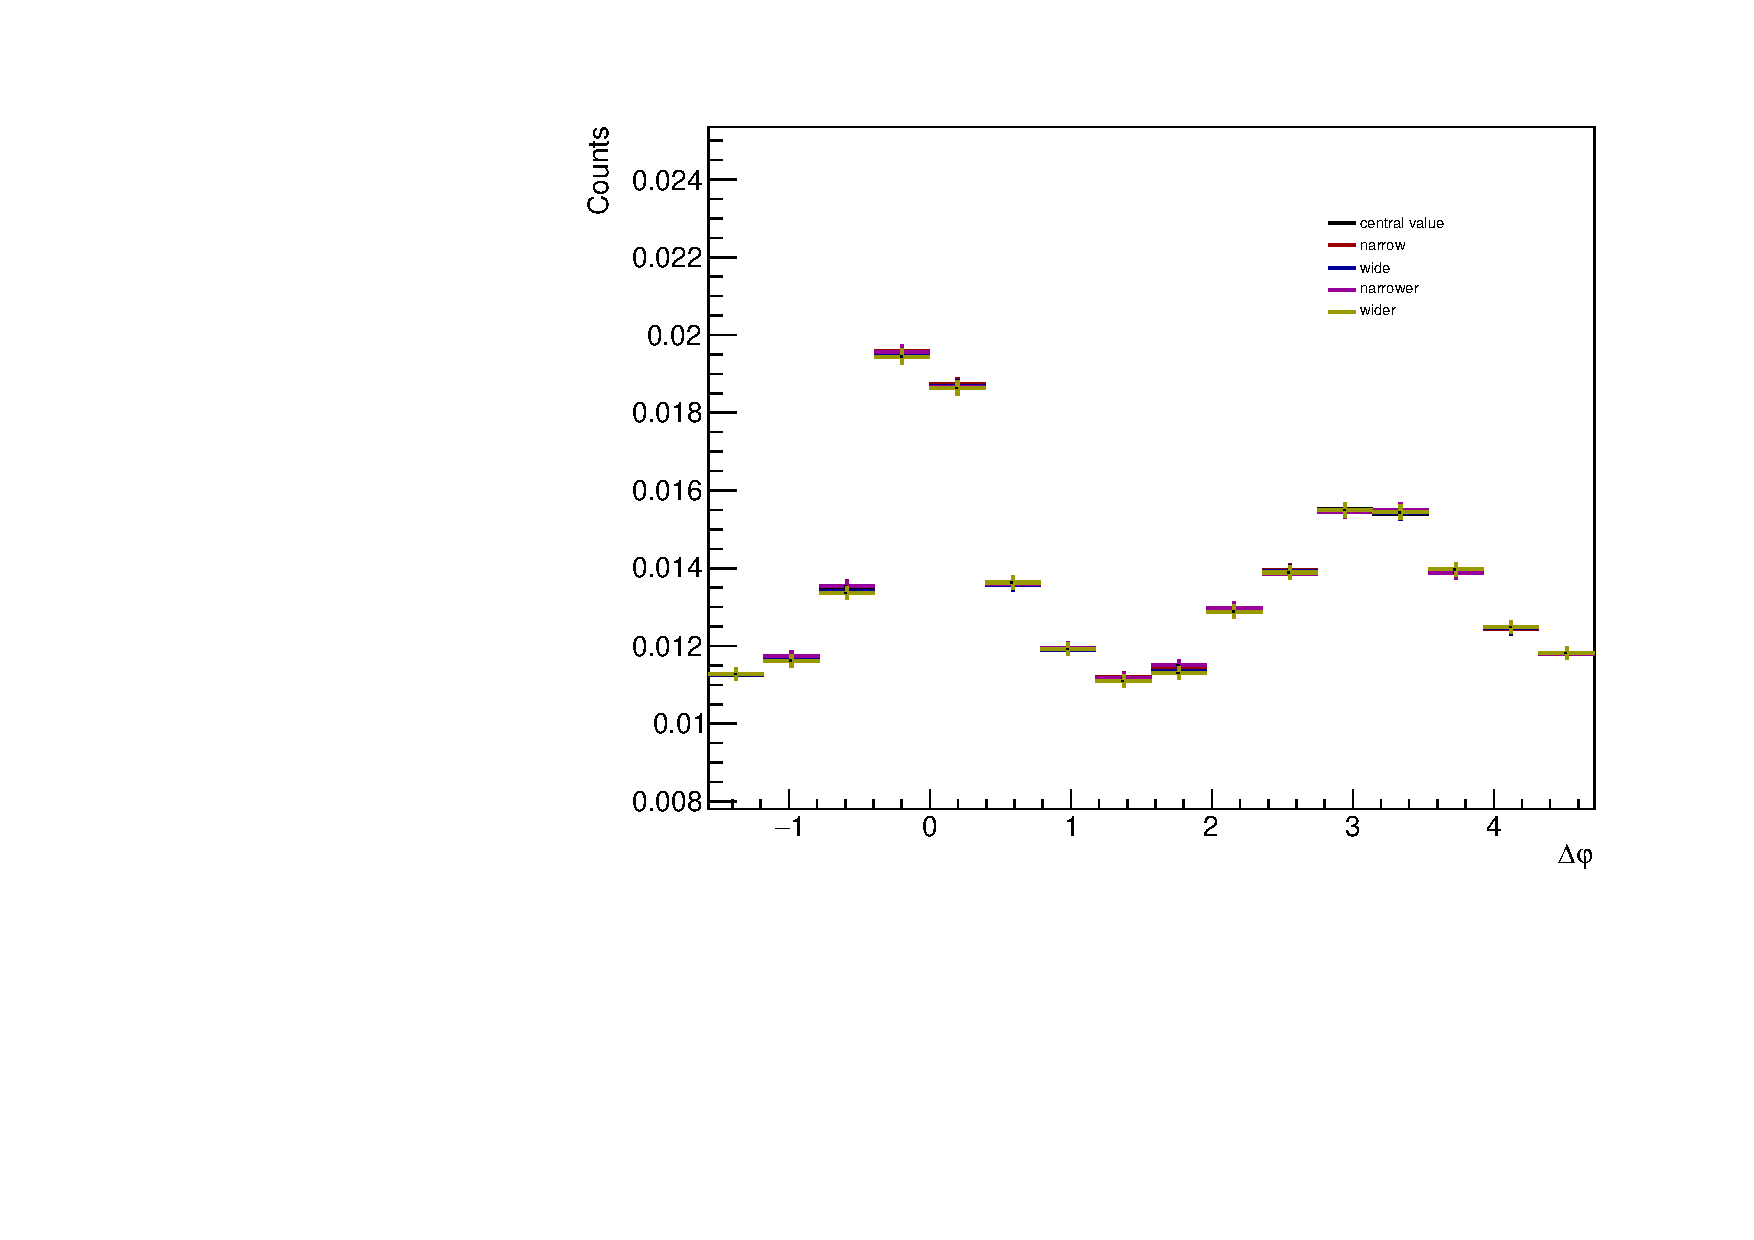
\includegraphics[width=0.49\textwidth]{figures/analysis/signal_variations_dphi_20_50_highpt.pdf}
    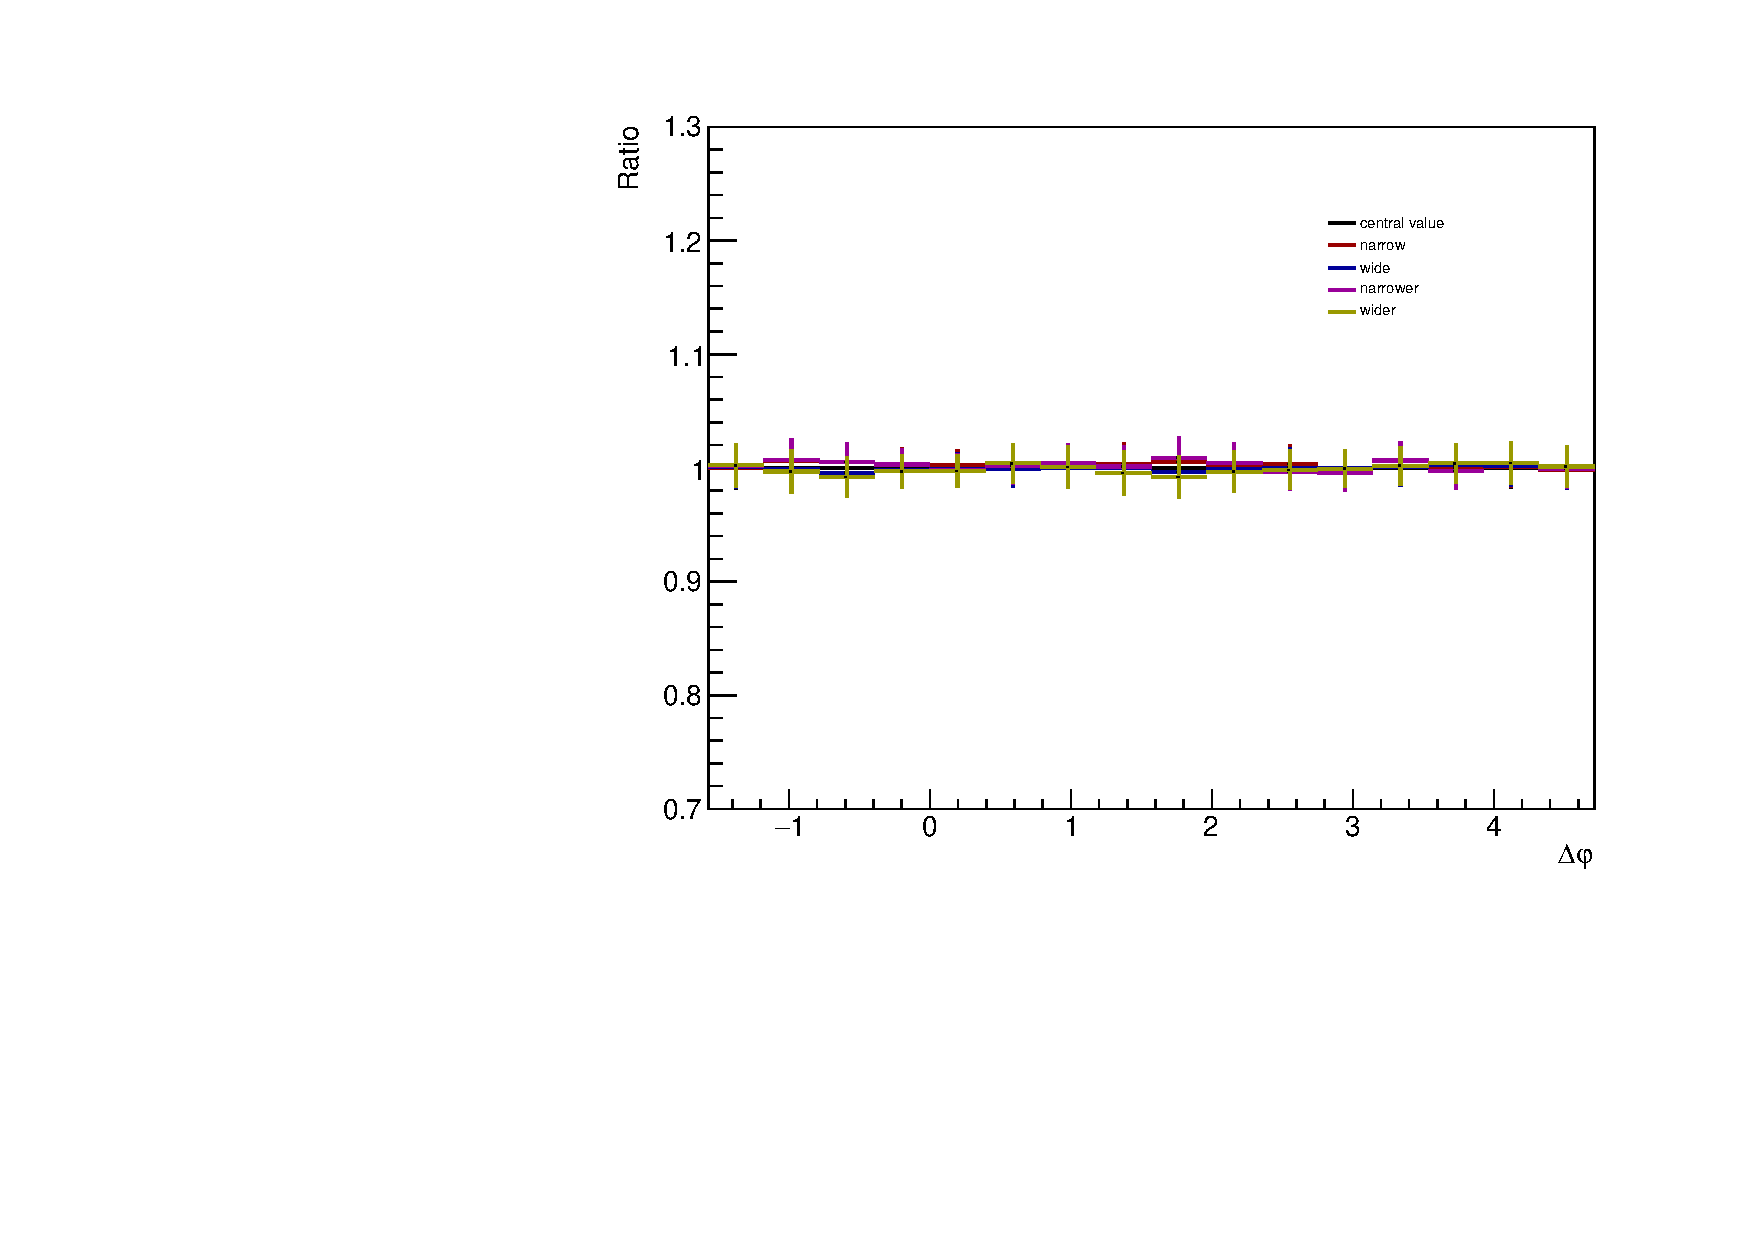
\includegraphics[width=0.49\textwidth]{figures/analysis/signal_variations_dphi_20_50_highpt_ratio.pdf}
    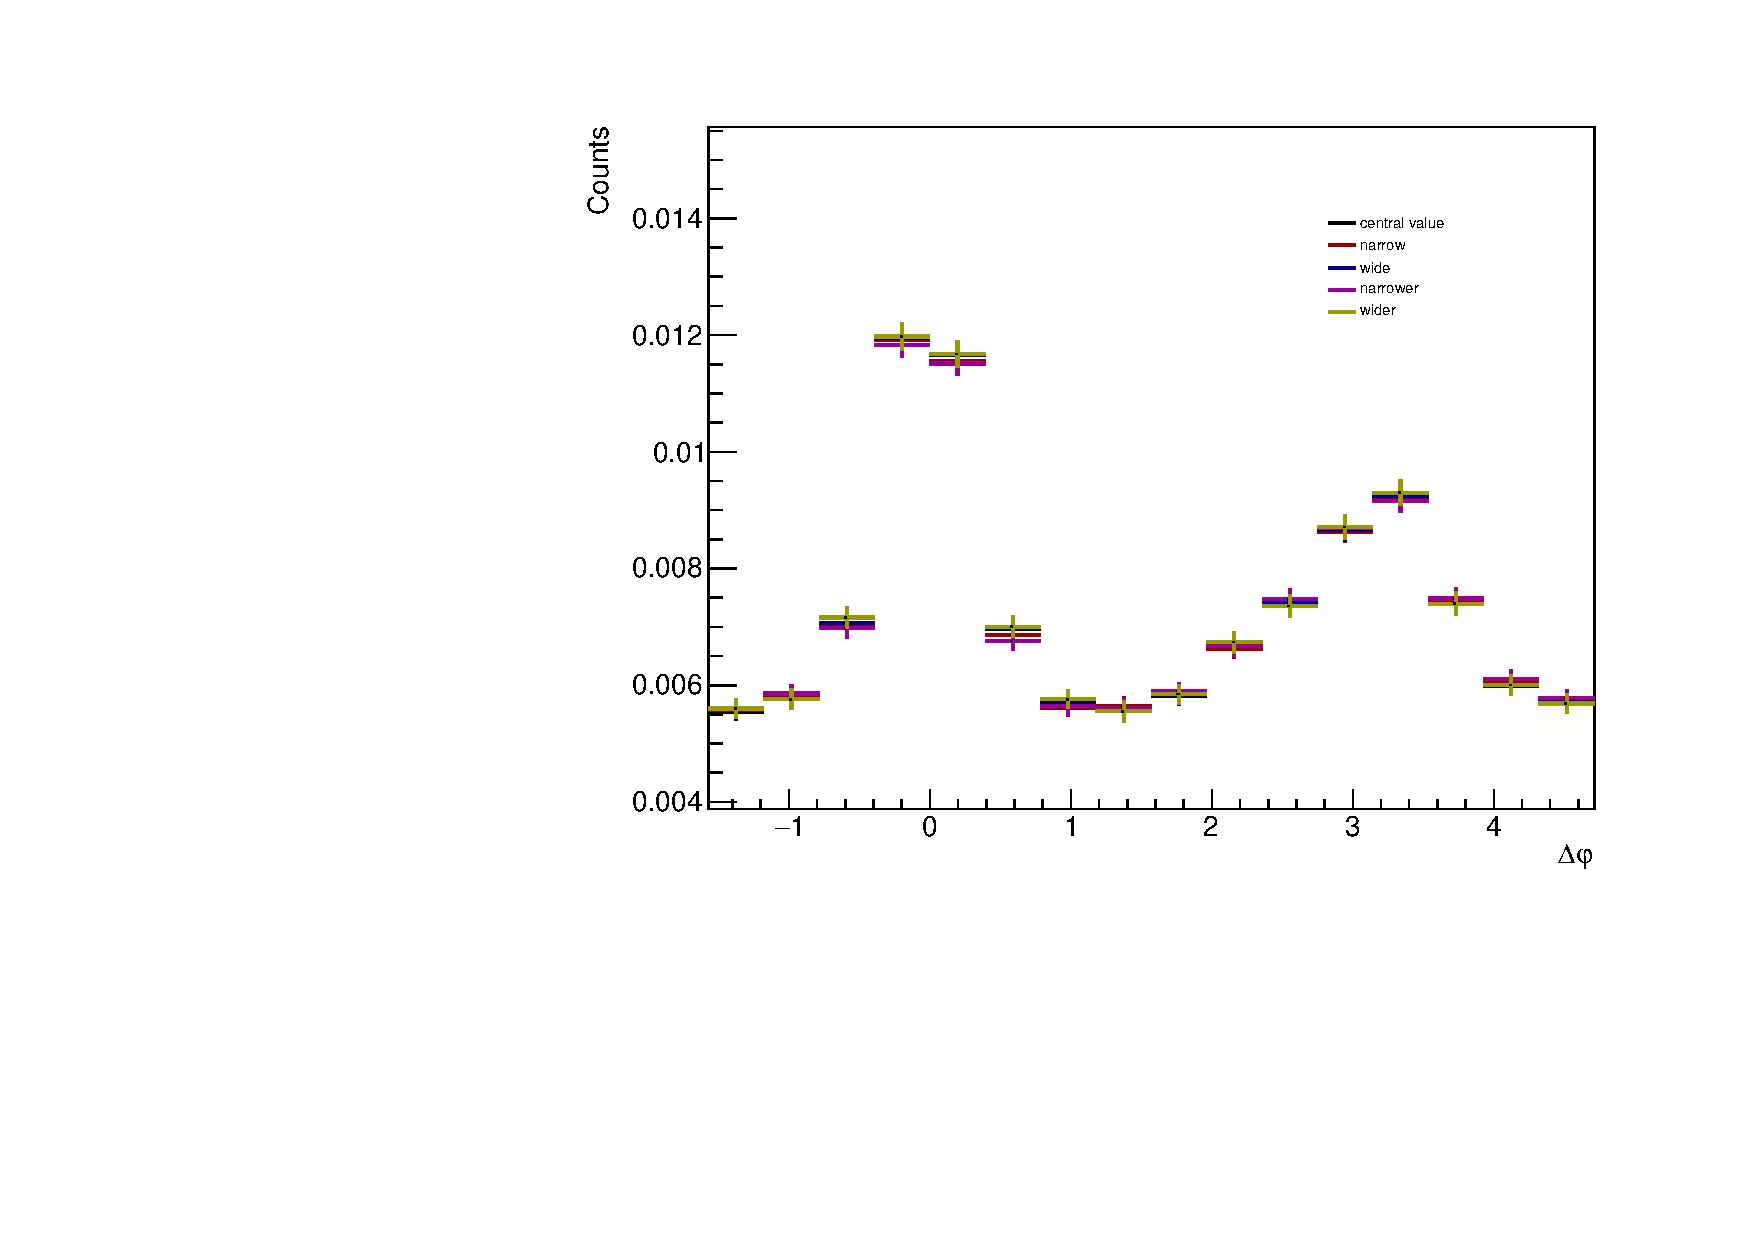
\includegraphics[width=0.49\textwidth]{figures/analysis/signal_variations_dphi_50_80_highpt.pdf}
    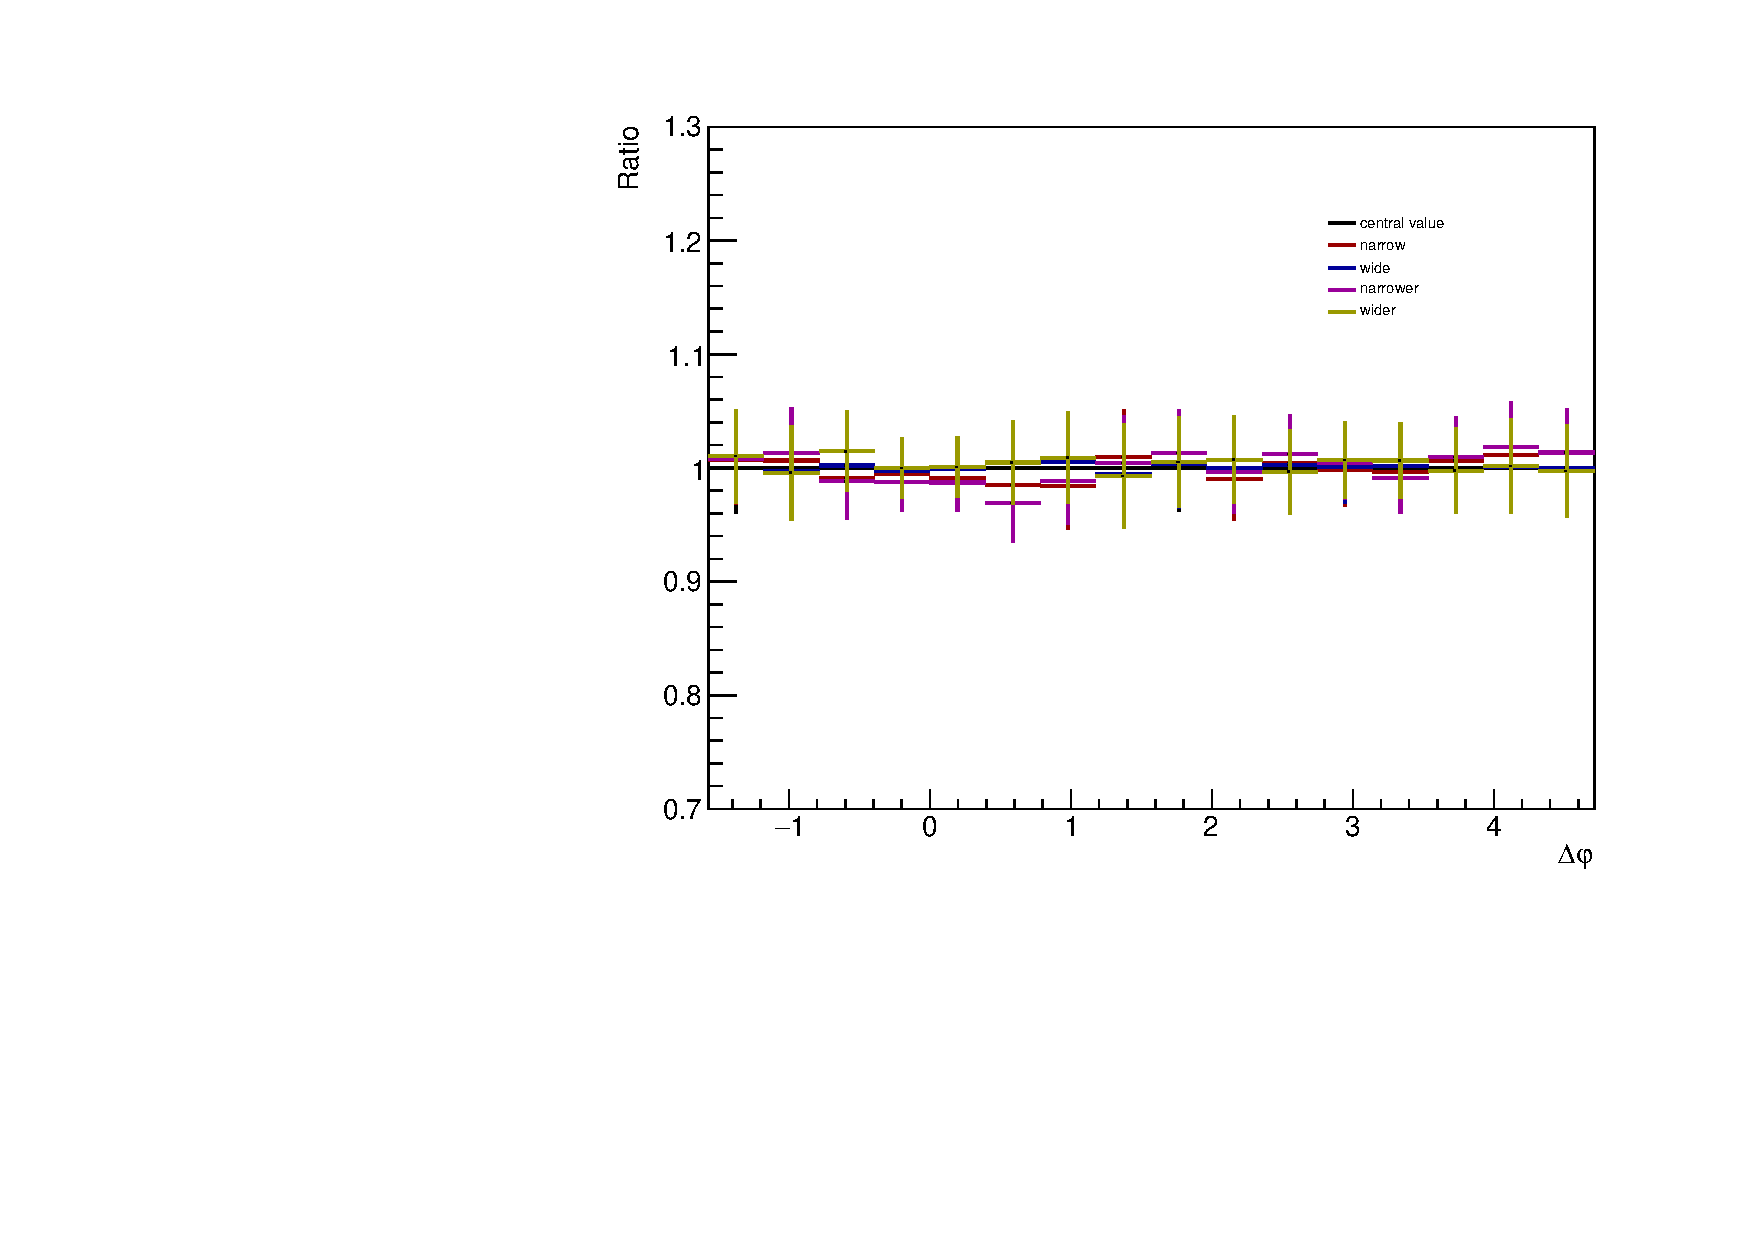
\includegraphics[width=0.49\textwidth]{figures/analysis/signal_variations_dphi_50_80_highpt_ratio.pdf}
    \caption{The h-\lmb $\Delta\varphi$ distributions within the 0-20\% (top), 20-50\% (middle), and 50-80\% (bottom) multiplicity bins in the higher associated \pt bin for each of the signal region variations (left) with the ratios to the nominal distribution (right).}
    \label{fig:signal_region_variations_highpt}
\end{figure}

\subsubsection{Sideband region selection}
The choice of sideband region also leaves a lot of room for reasonable variation: all that is required is that the region is 1) large enough to produce a smooth h-p$\pi$ distribution with minimal statistical fluctuations and 2) close enough to the signal region that the p$\pi$ pairs are kinematically similar to those in the background of the signal region. As long as these requirements are met, the final result should not be very dependent on the choice of sideband region. To investigate the effects of changing the sideband region, the variations presented in Table~\ref{tab:sideband_region_variations} are considered. The measured $\Delta\varphi$ distributions and variation/nominal ratios for each sideband region variation in each multiplicity and associated \pt bin are shown in Figures \ref{fig:sideband_region_variations_lowpt} (lower \pt) and \ref{fig:sideband_region_variations_highpt} (higher \pt). The result is even less deviation from the nominal distribution than the signal region variations, with the average deviation being closer to ~1\%. Again, no significant dependence is observed on $\Delta\varphi$, so the systematic uncertainty is calculated as the RMS of the percent change from each variation across every $\Delta\varphi$ bin.

\begin{table}[ht]
    \centering
    \caption{The variations of the \lmb invariant mass sideband region considered for this analysis. Note that the ``shifted left'' sideband falls on the opposite (left) side of the signal region.}
    \label{tab:sideband_region_variations}
    \begin{tabular}{l c}
        \hline
        Variation name & Sideband range (GeV/$c^2$) \\
        \hline
        Narrow & $1.135 < M_{p\pi} < 1.145$ \\
        Wide & $1.135 < M_{p\pi} < 1.16$ \\
        Shifted left & $1.086 < M_{p\pi} < 1.098$ \\
        Shifted right & $1.14 < M_{p\pi} < 1.155$ \\
        \hline
    \end{tabular}
\end{table}

\begin{figure}[ht]
    \centering
    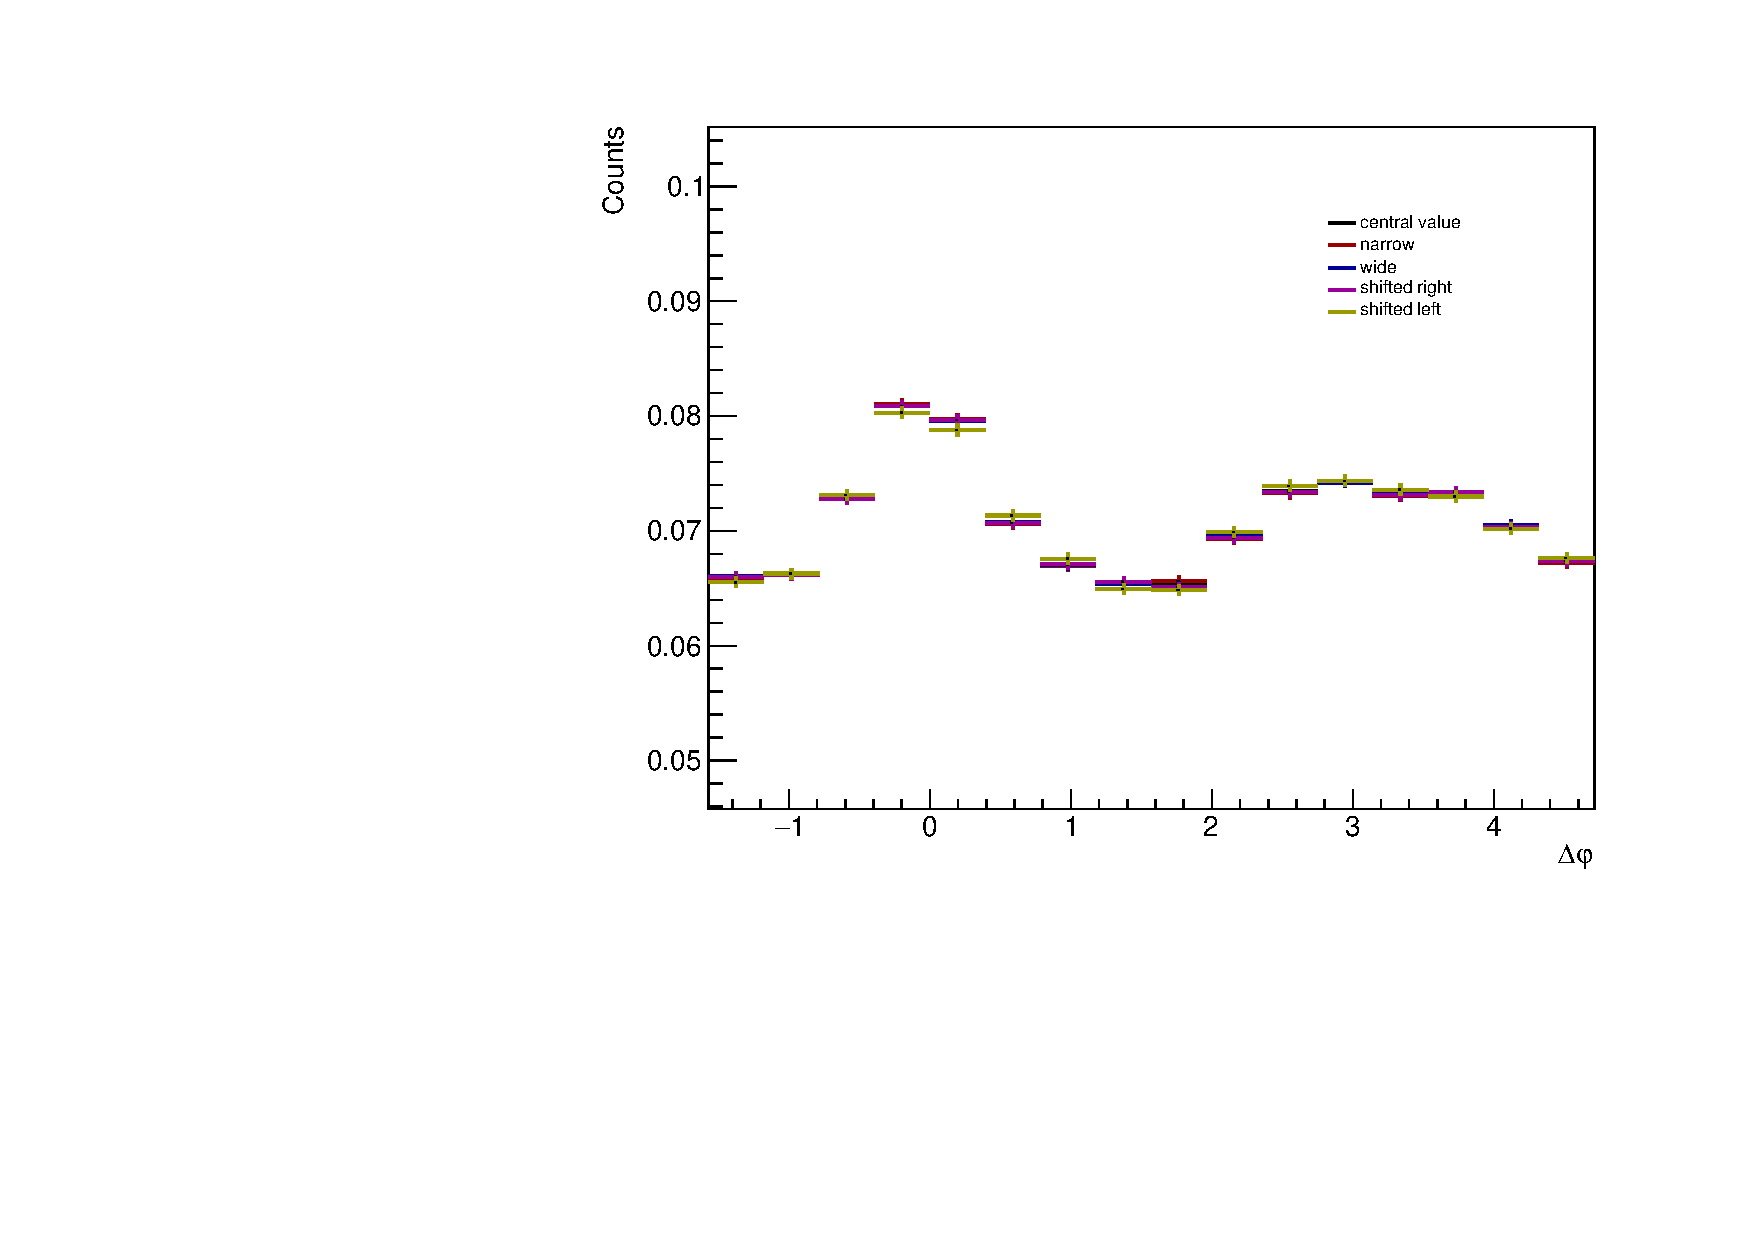
\includegraphics[width=0.49\textwidth]{figures/analysis/sideband_variations_dphi_0_20_lowpt.pdf}
    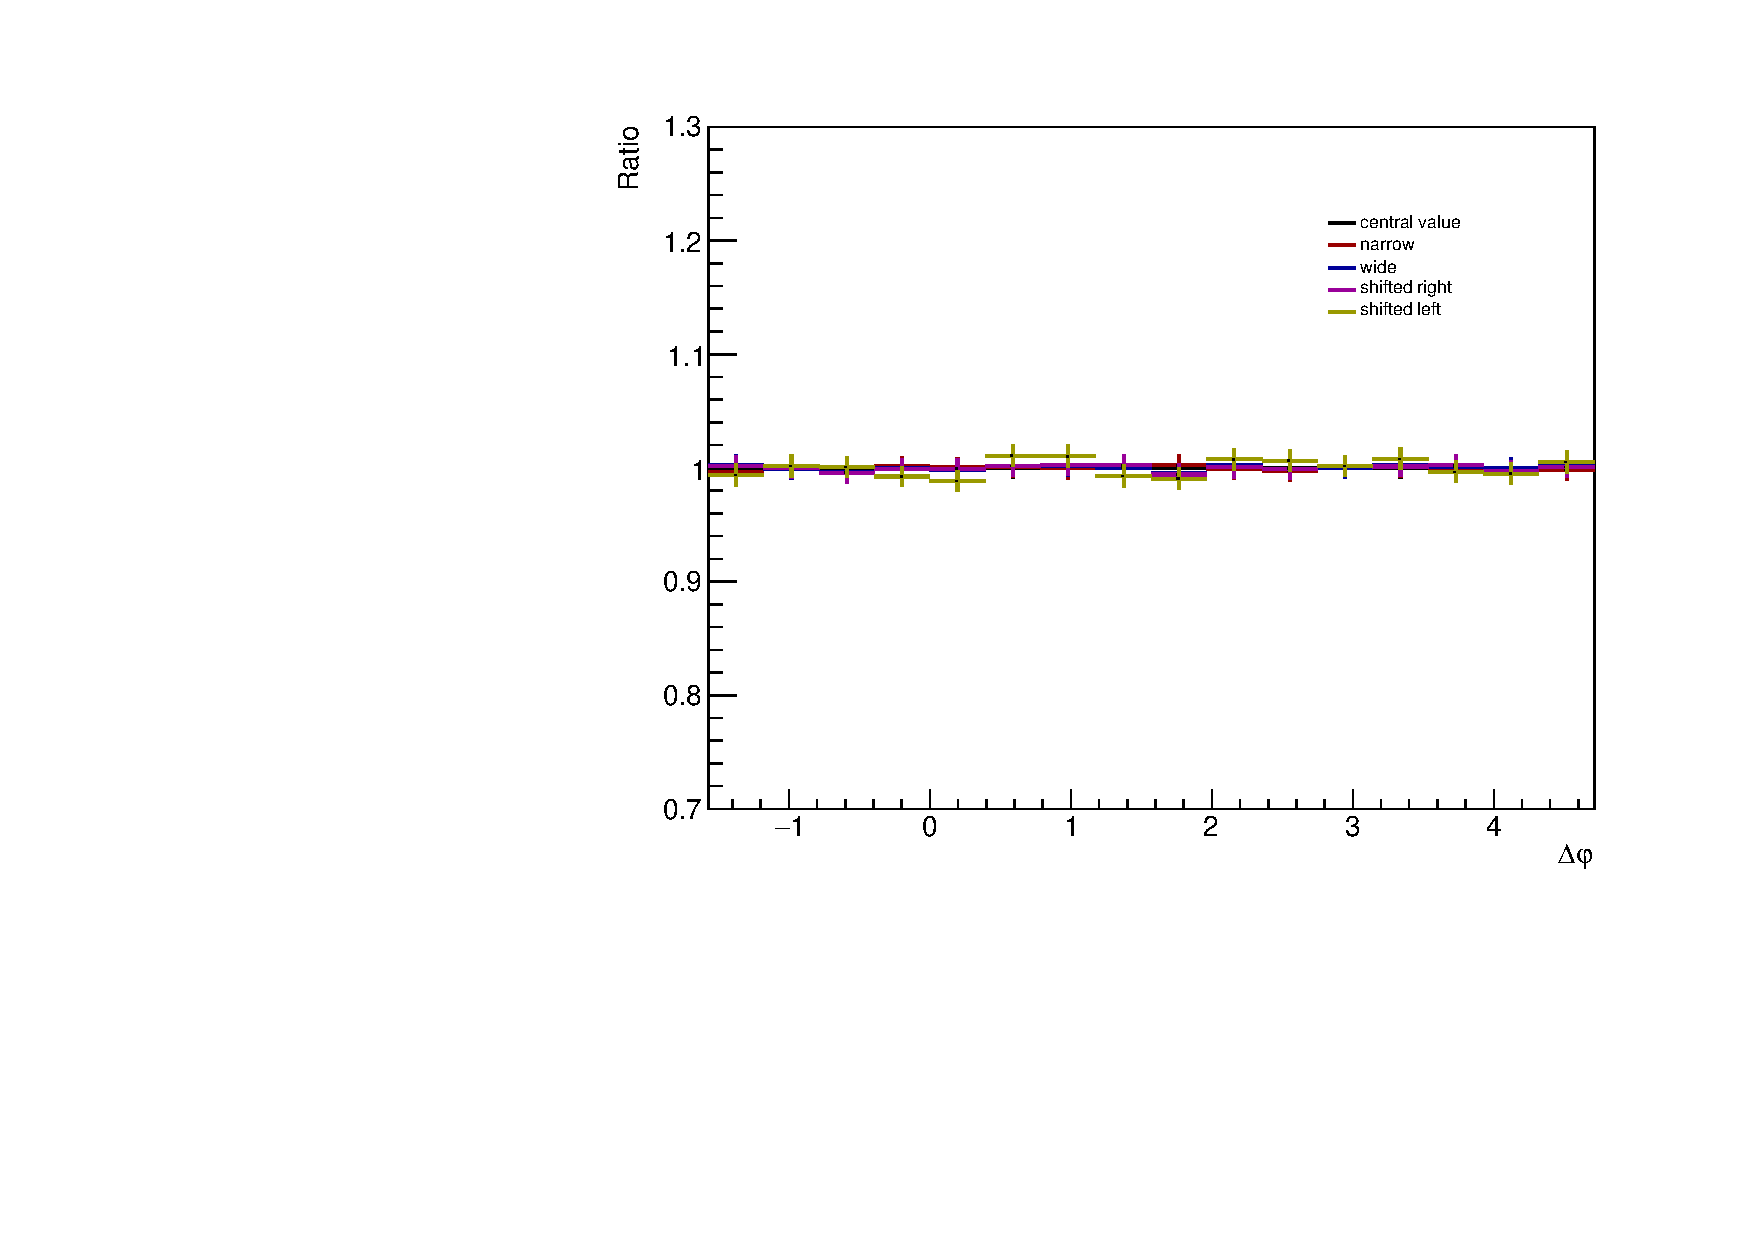
\includegraphics[width=0.49\textwidth]{figures/analysis/sideband_variations_dphi_0_20_lowpt_ratio.pdf}
    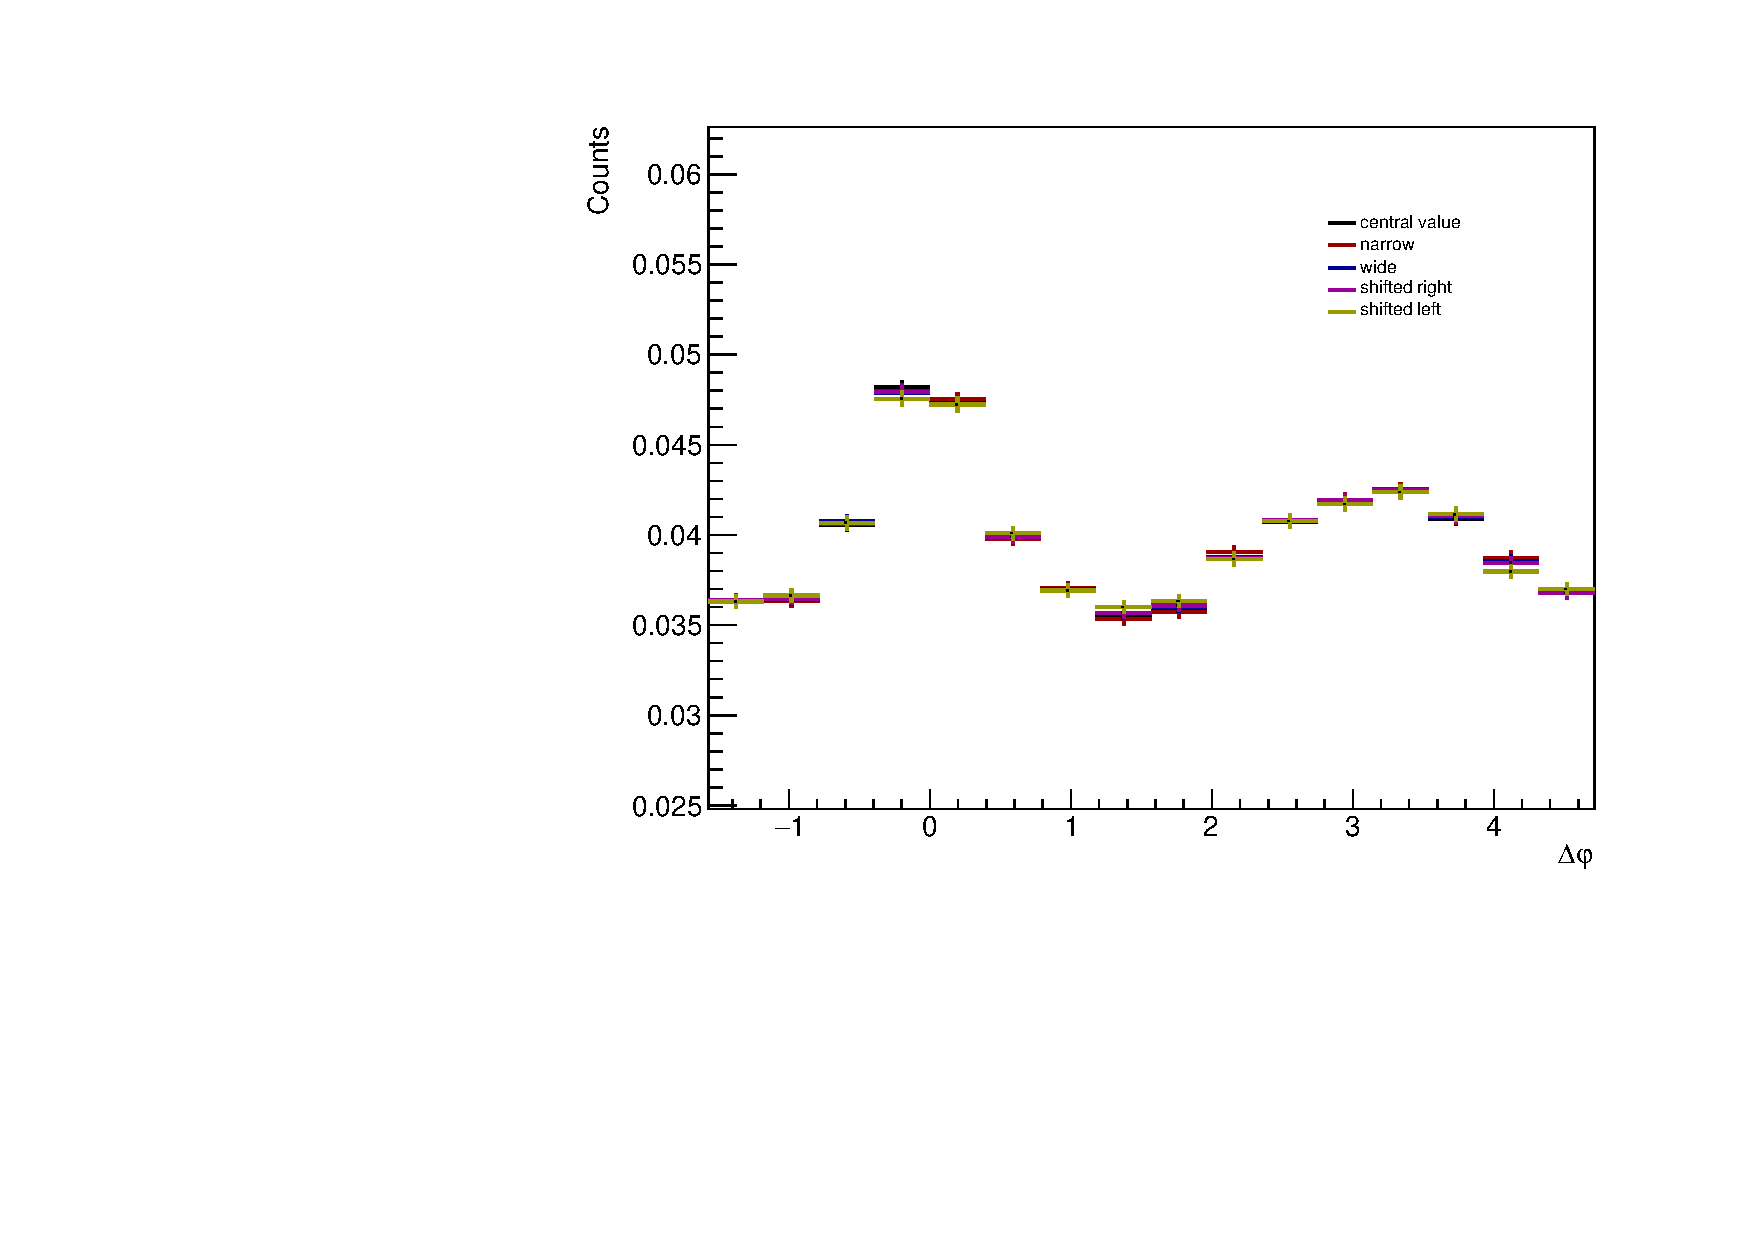
\includegraphics[width=0.49\textwidth]{figures/analysis/sideband_variations_dphi_20_50_lowpt.pdf}
    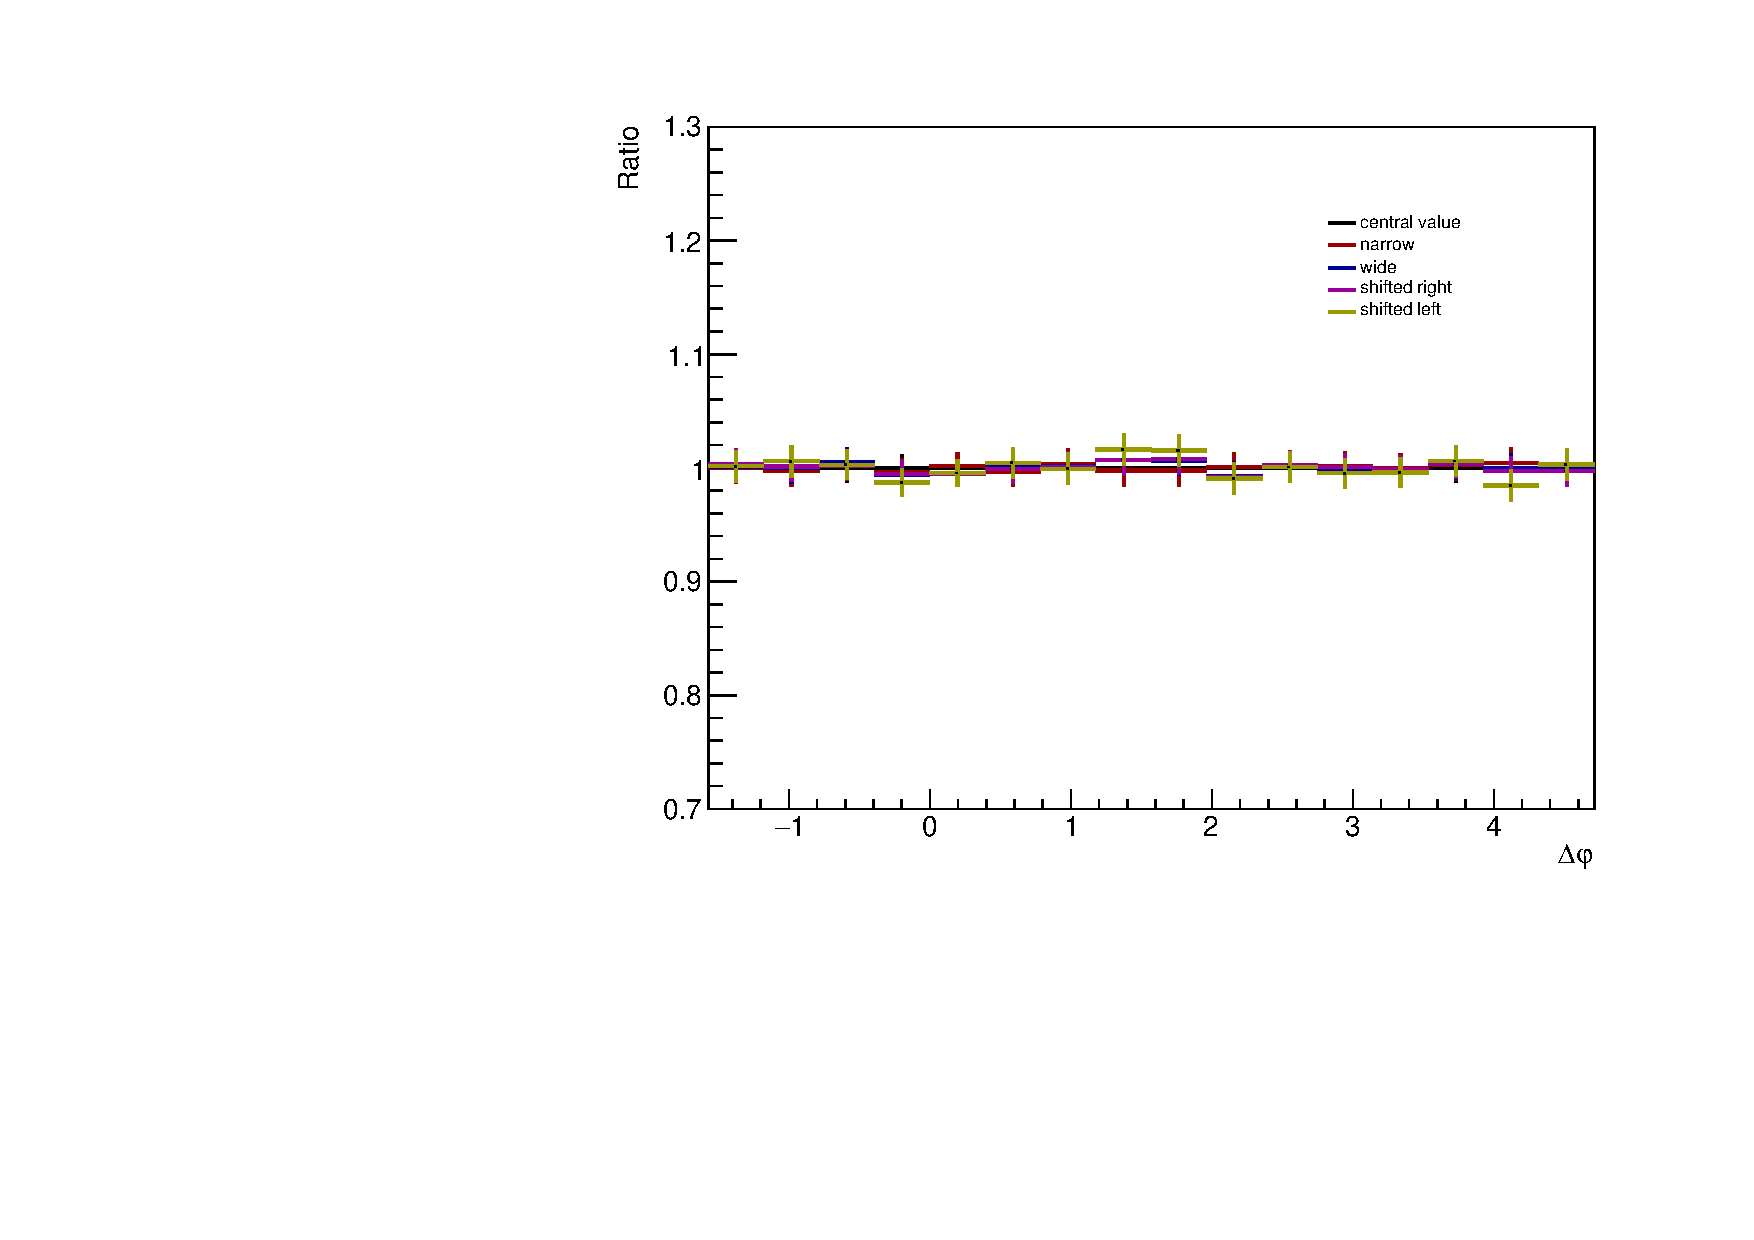
\includegraphics[width=0.49\textwidth]{figures/analysis/sideband_variations_dphi_20_50_lowpt_ratio.pdf}
    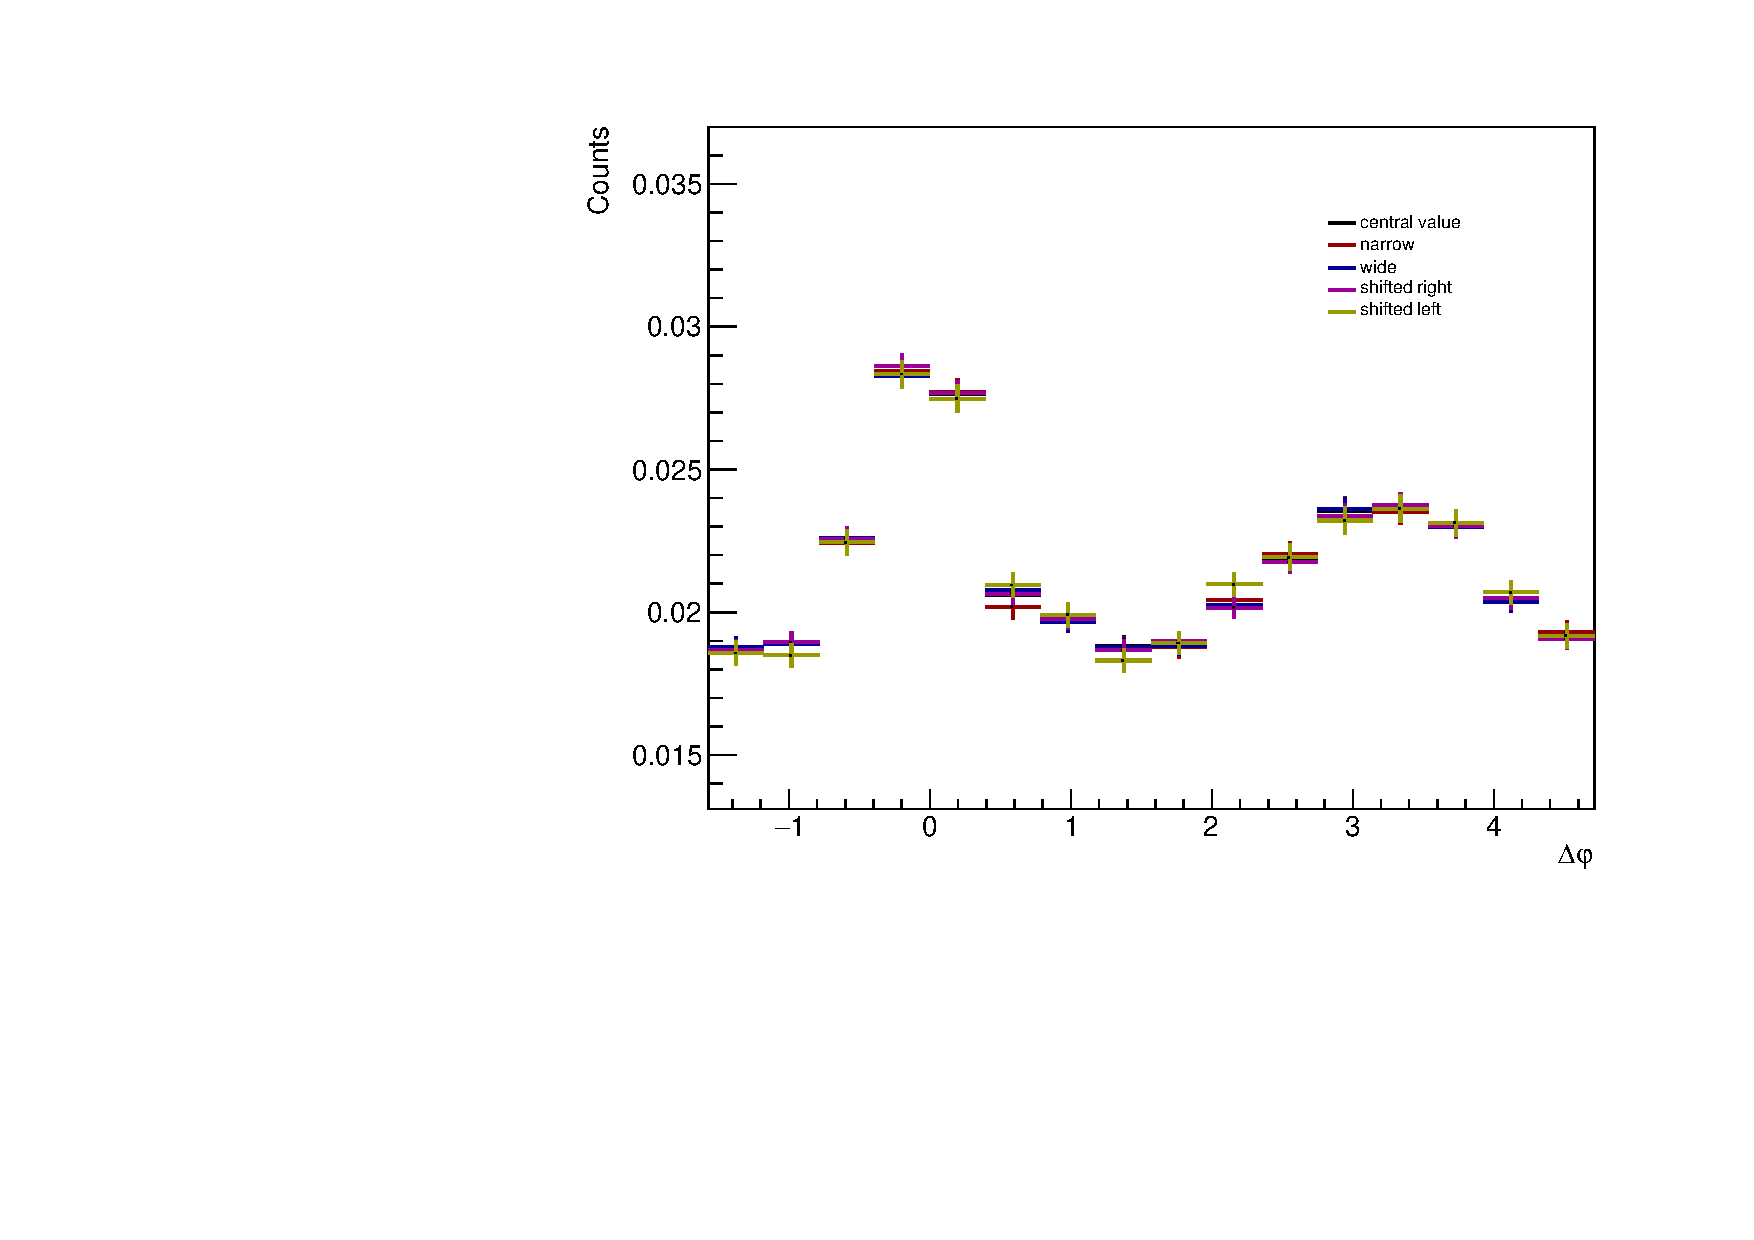
\includegraphics[width=0.49\textwidth]{figures/analysis/sideband_variations_dphi_50_80_lowpt.pdf}
    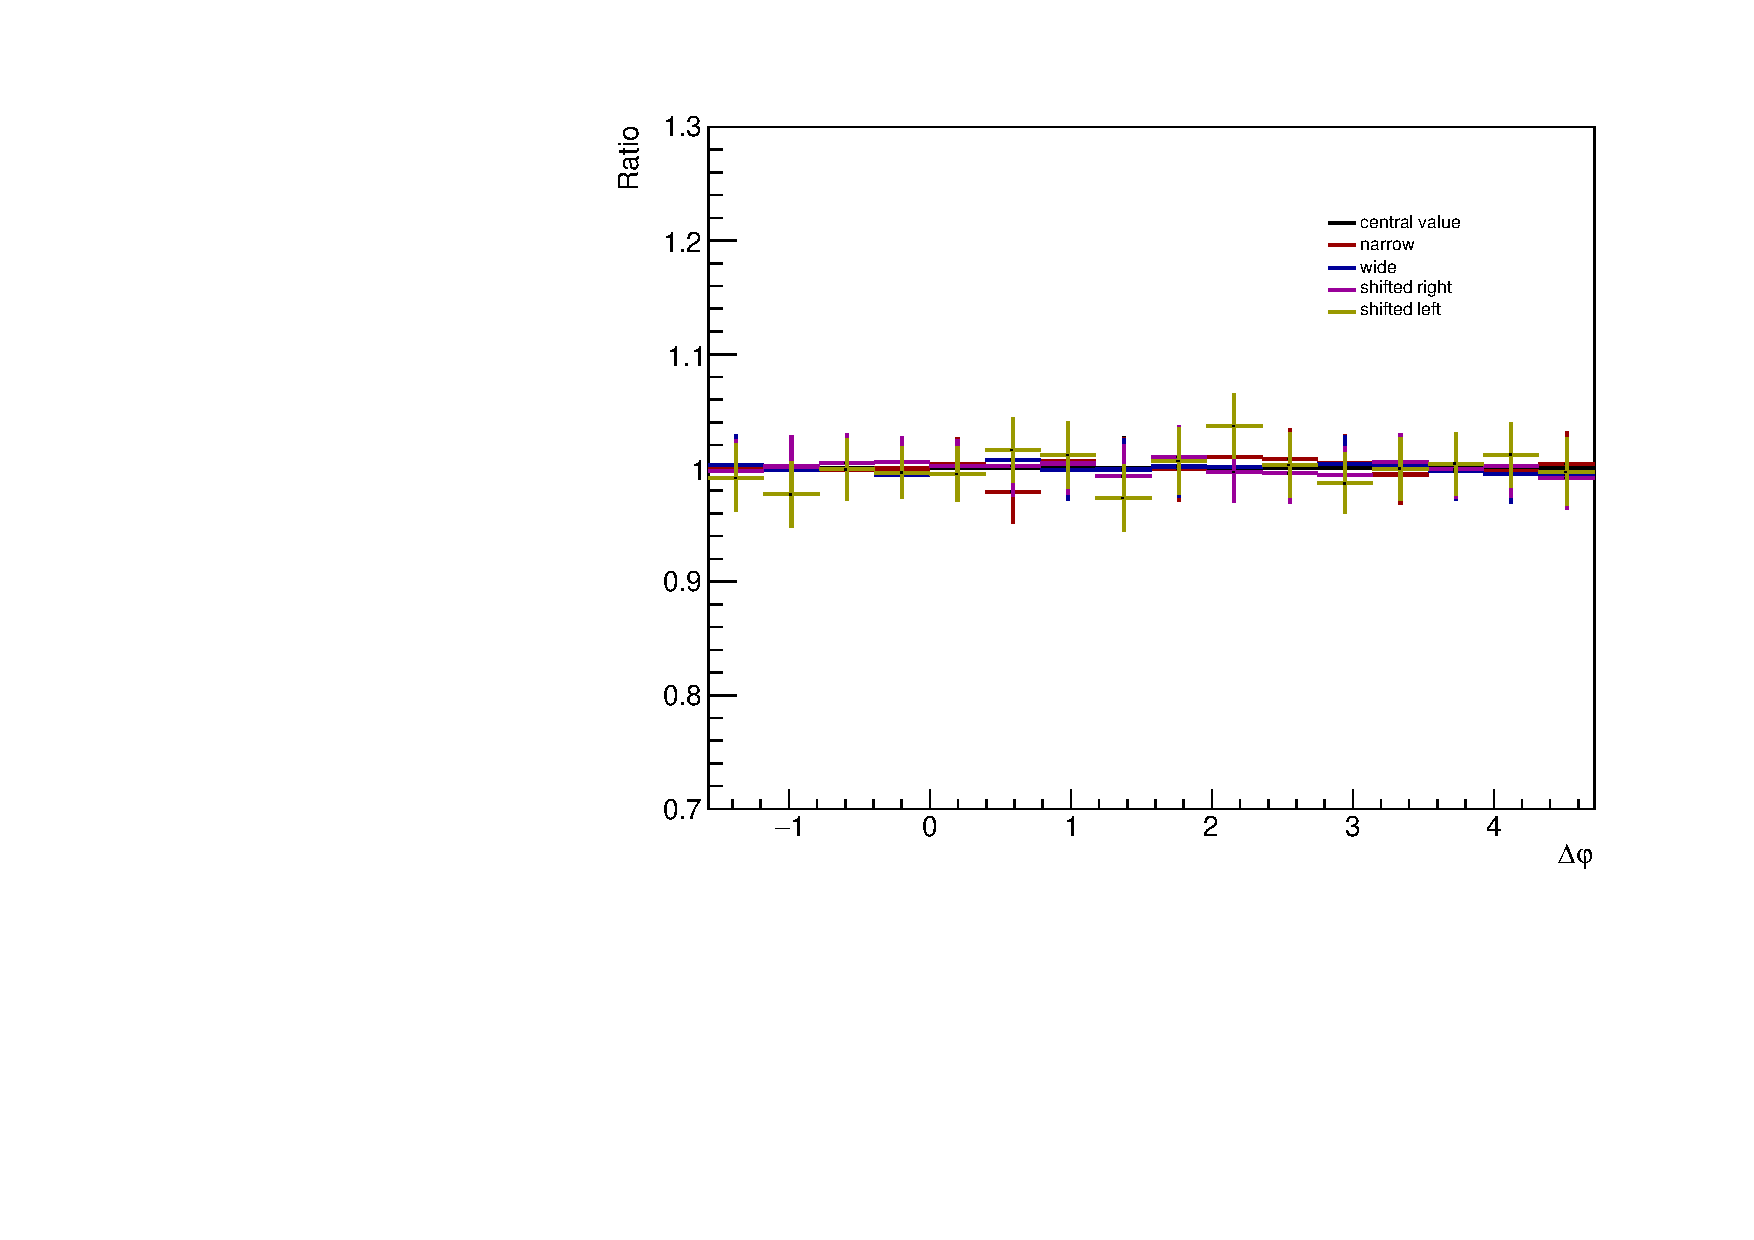
\includegraphics[width=0.49\textwidth]{figures/analysis/sideband_variations_dphi_50_80_lowpt_ratio.pdf}
    \caption{The h-\lmb $\Delta\varphi$ distributions within the 0-20\% (top), 20-50\% (middle), and 50-80\% (bottom) multiplicity bins in the lower associated \pt bin for each of the sideband region variations (left) with the ratios to the nominal distribution (right).}
    \label{fig:sideband_region_variations_lowpt}
\end{figure}

\begin{figure}[ht]
    \centering
    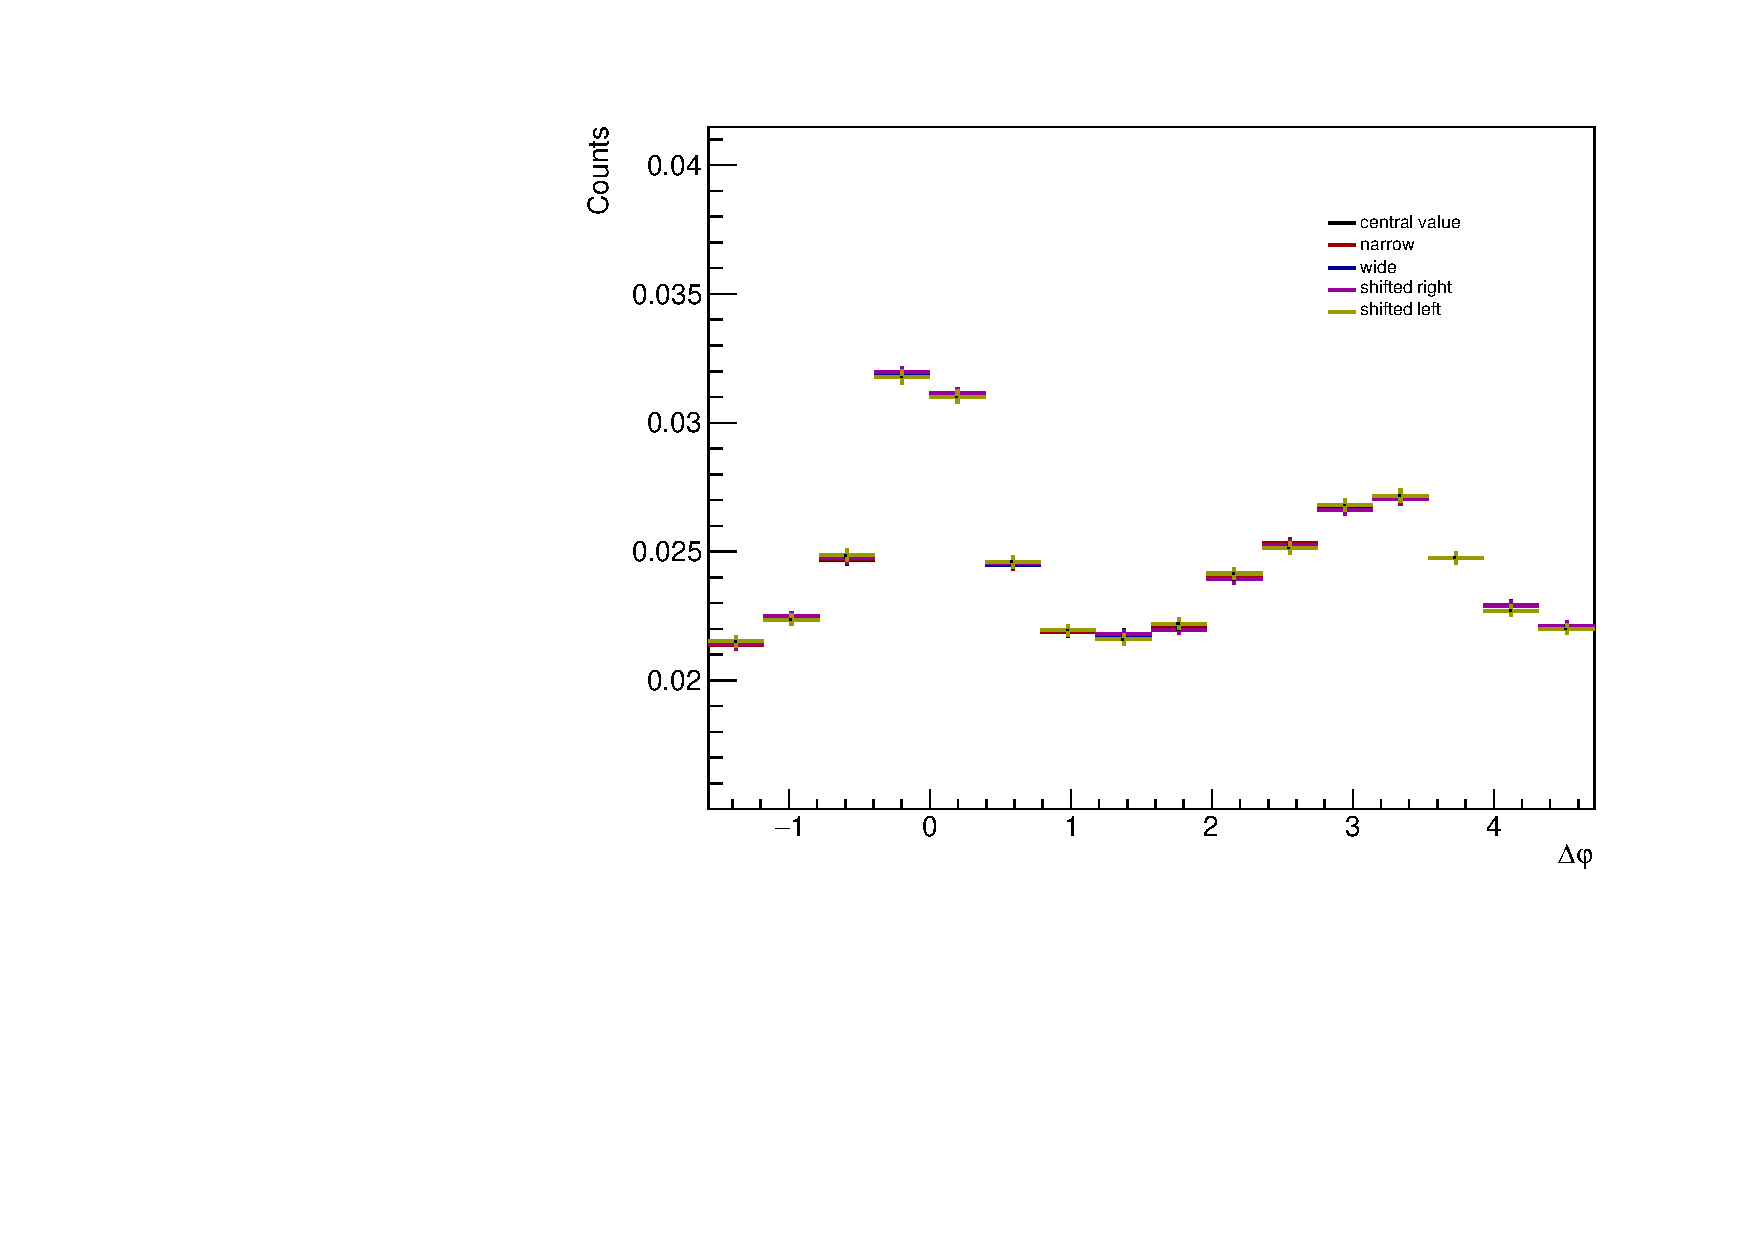
\includegraphics[width=0.49\textwidth]{figures/analysis/sideband_variations_dphi_0_20_highpt.pdf}
    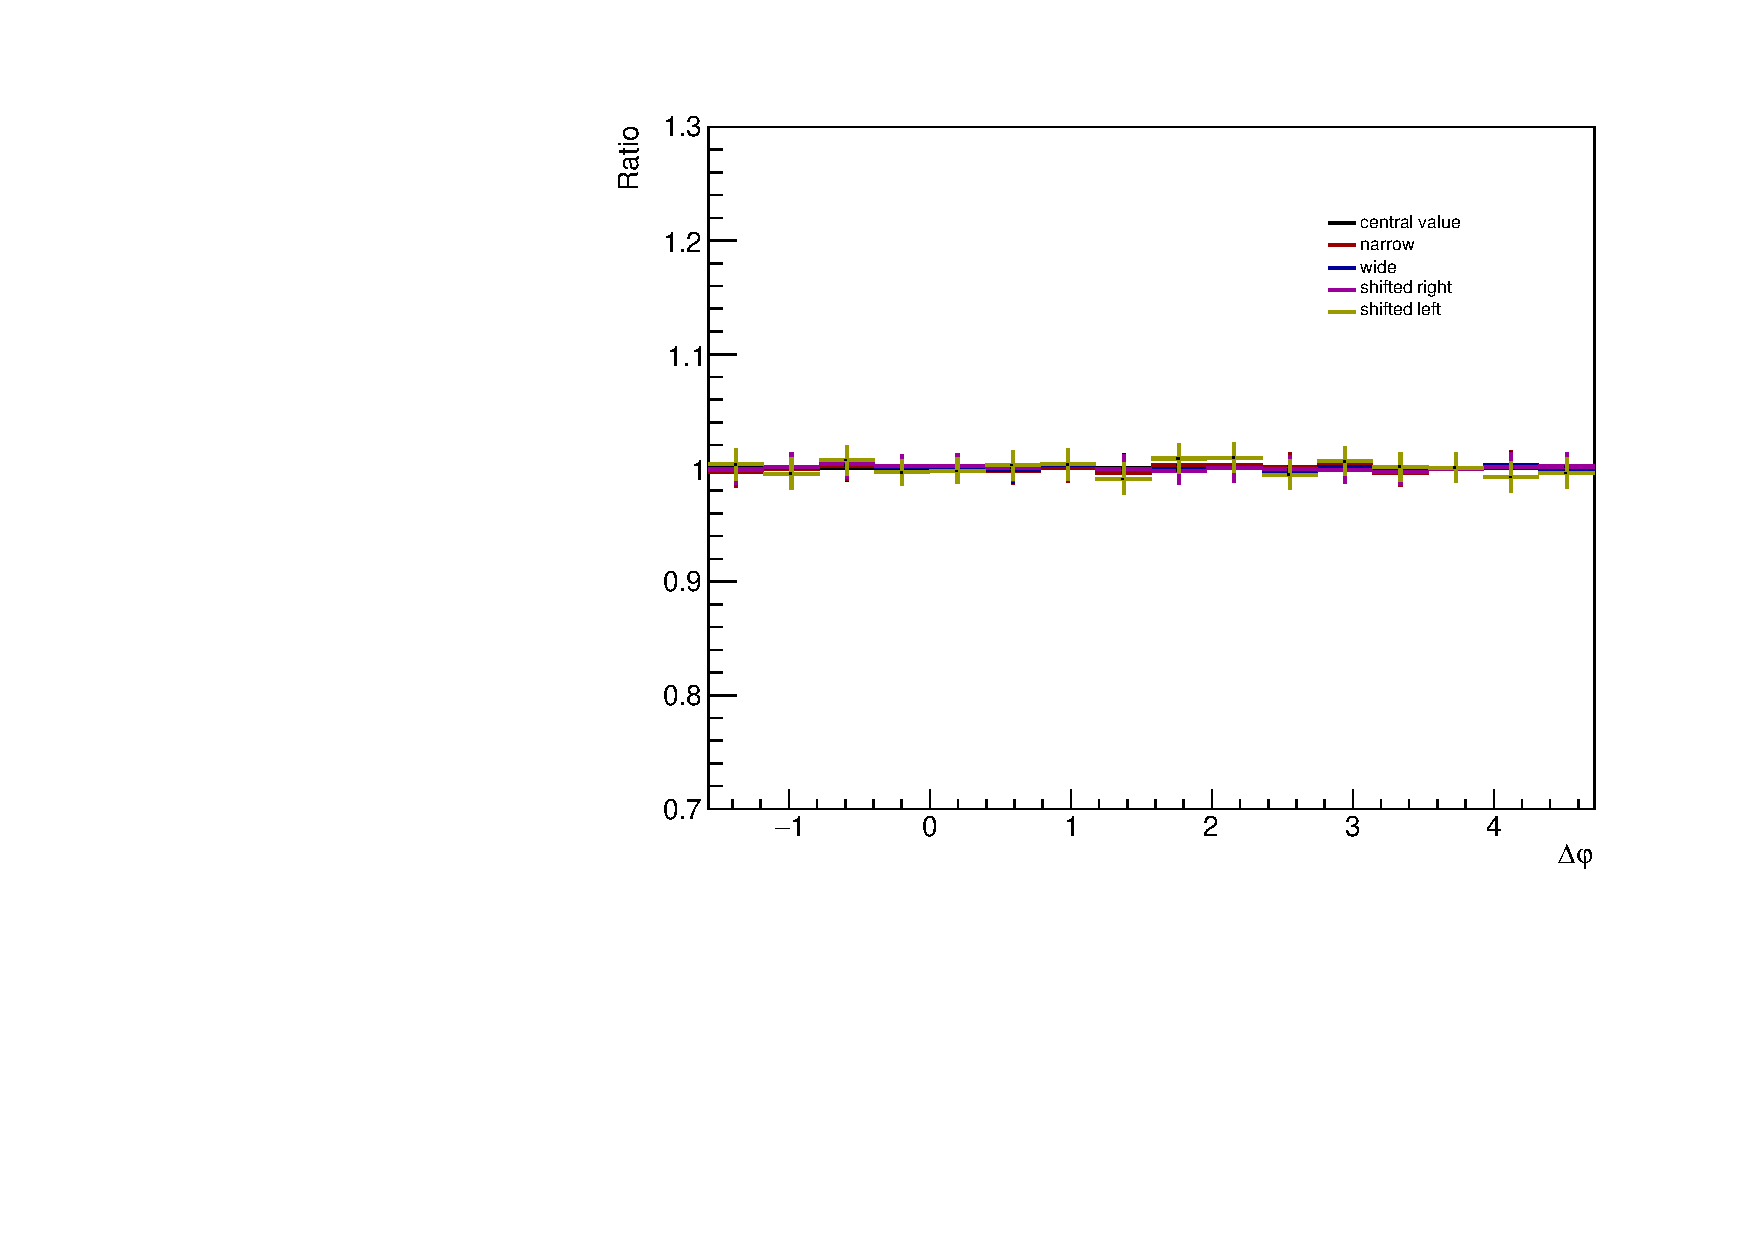
\includegraphics[width=0.49\textwidth]{figures/analysis/sideband_variations_dphi_0_20_highpt_ratio.pdf}
    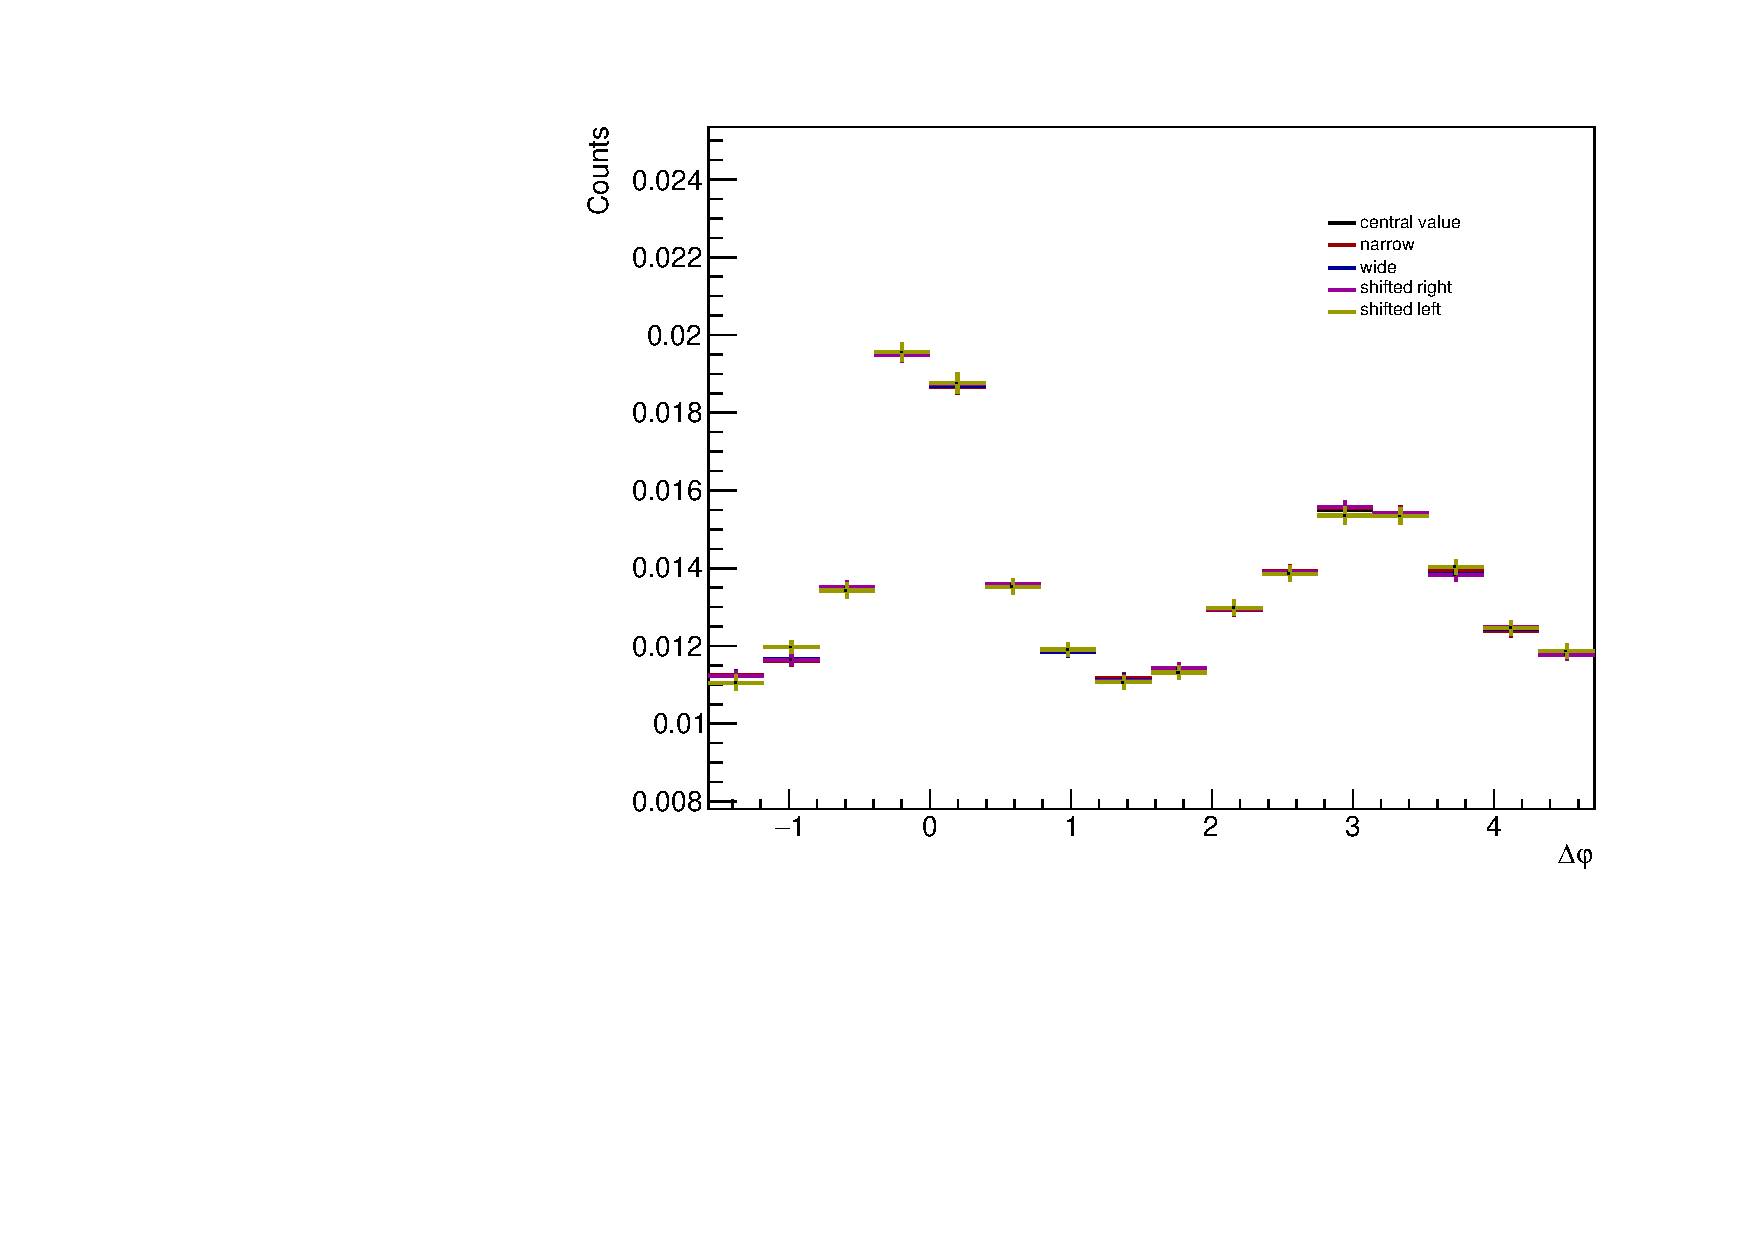
\includegraphics[width=0.49\textwidth]{figures/analysis/sideband_variations_dphi_20_50_highpt.pdf}
    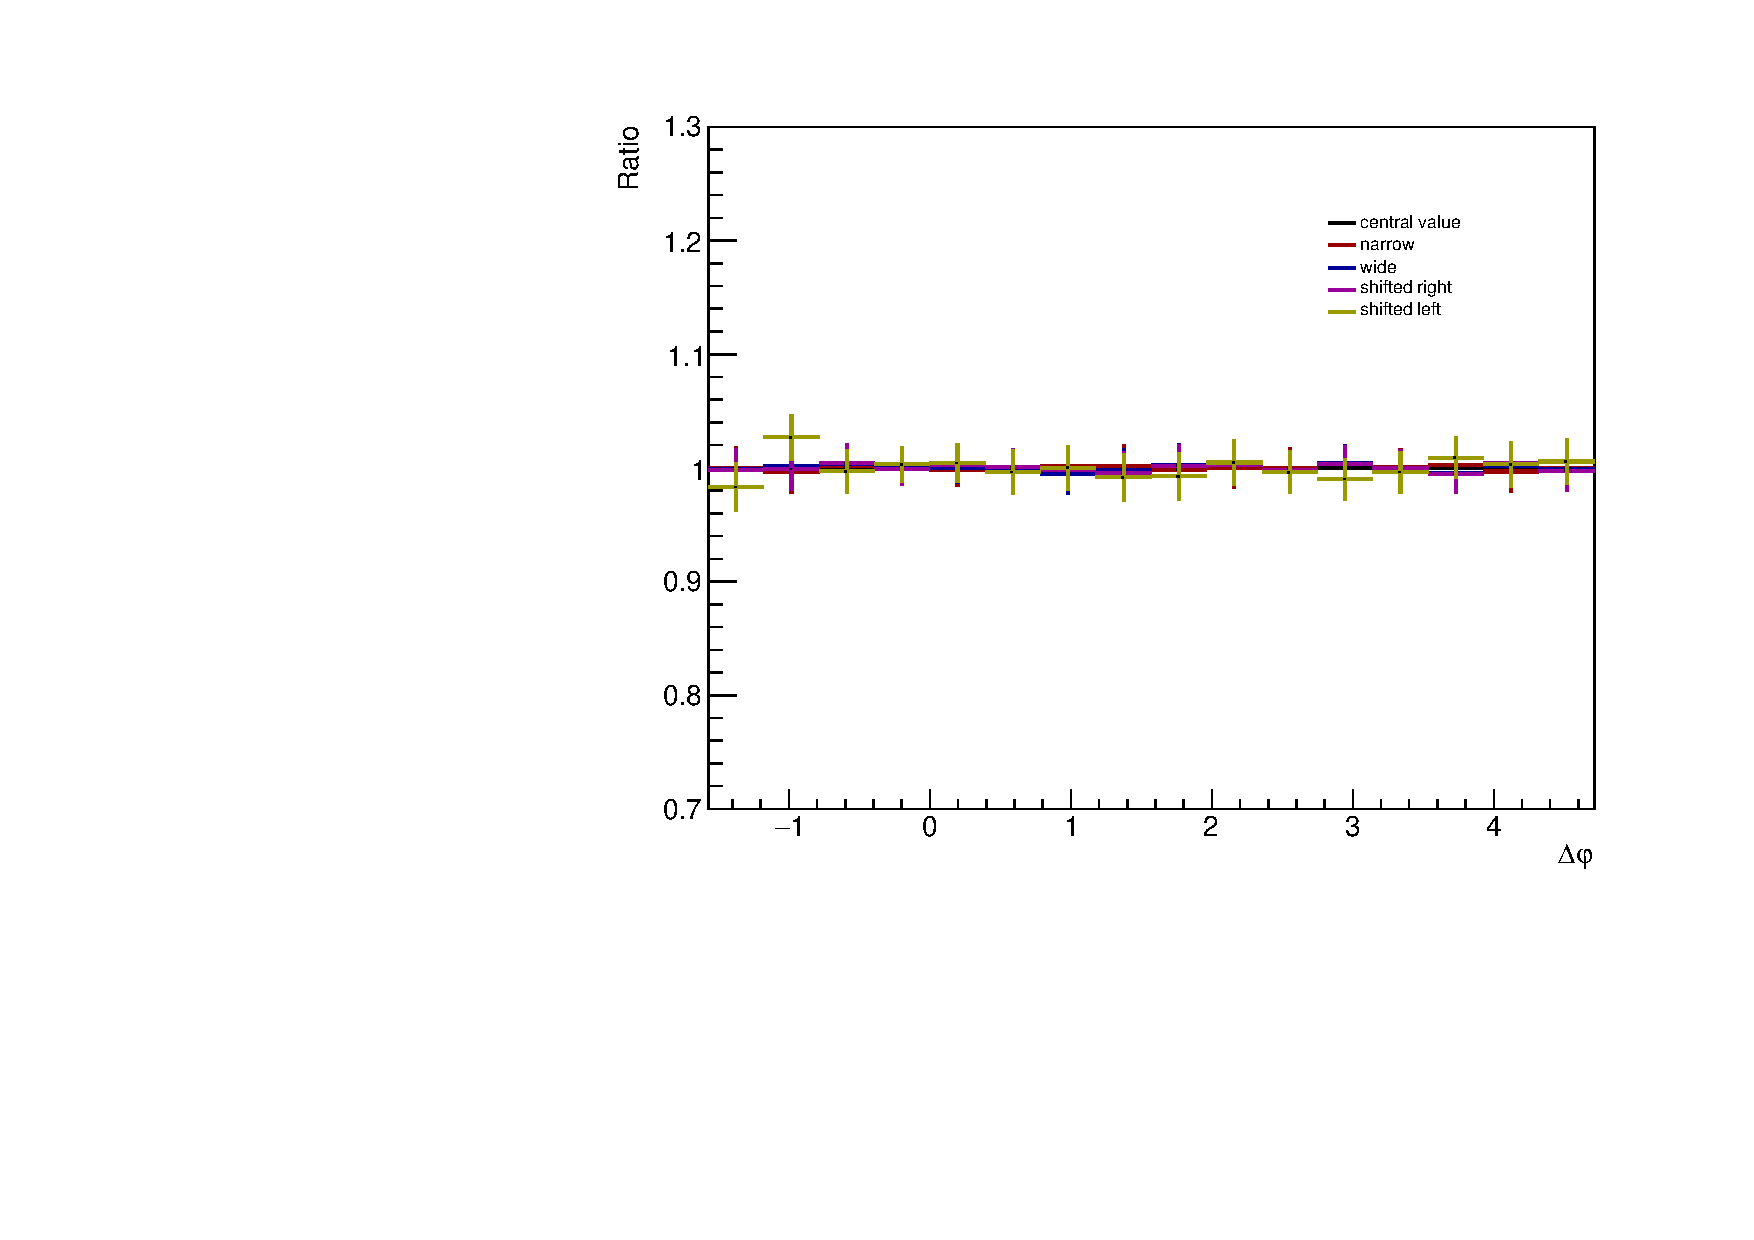
\includegraphics[width=0.49\textwidth]{figures/analysis/sideband_variations_dphi_20_50_highpt_ratio.pdf}
    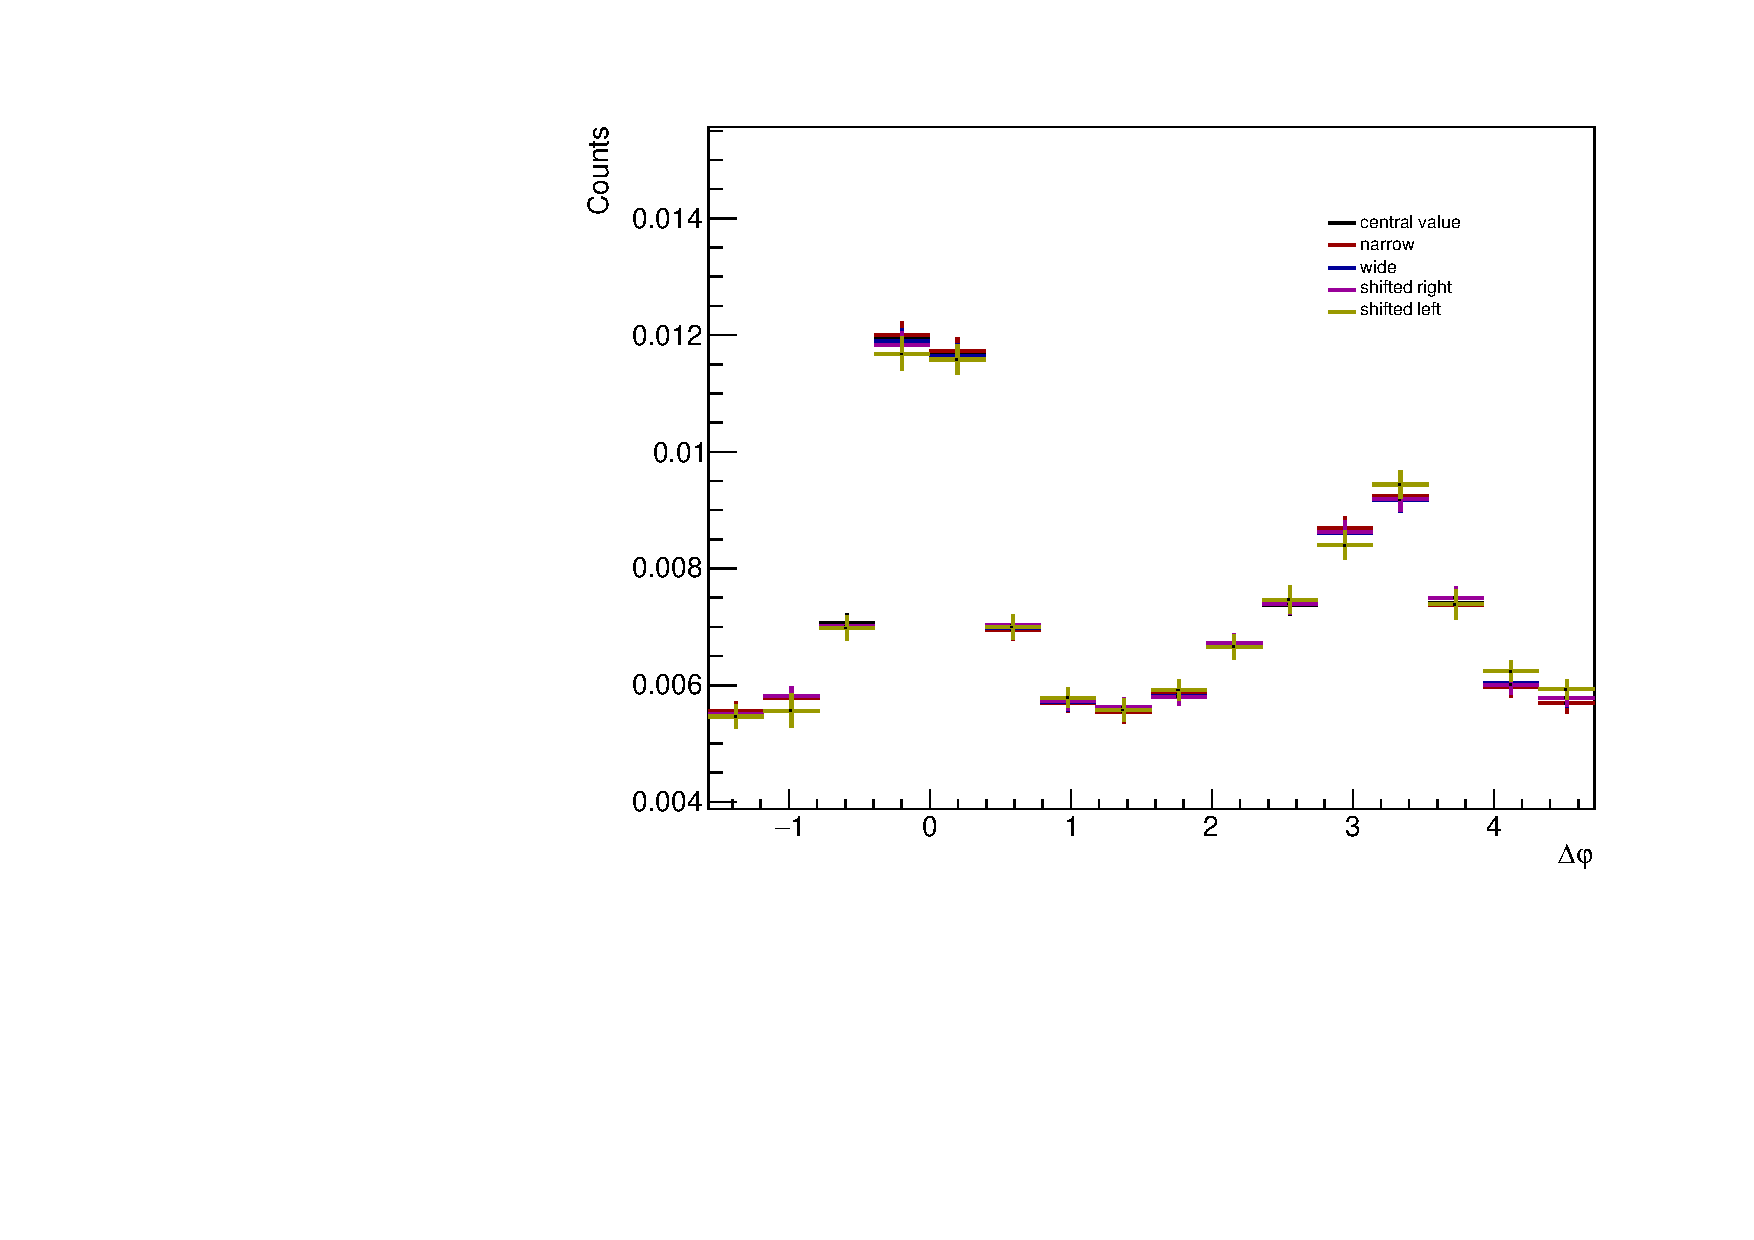
\includegraphics[width=0.49\textwidth]{figures/analysis/sideband_variations_dphi_50_80_highpt.pdf}
    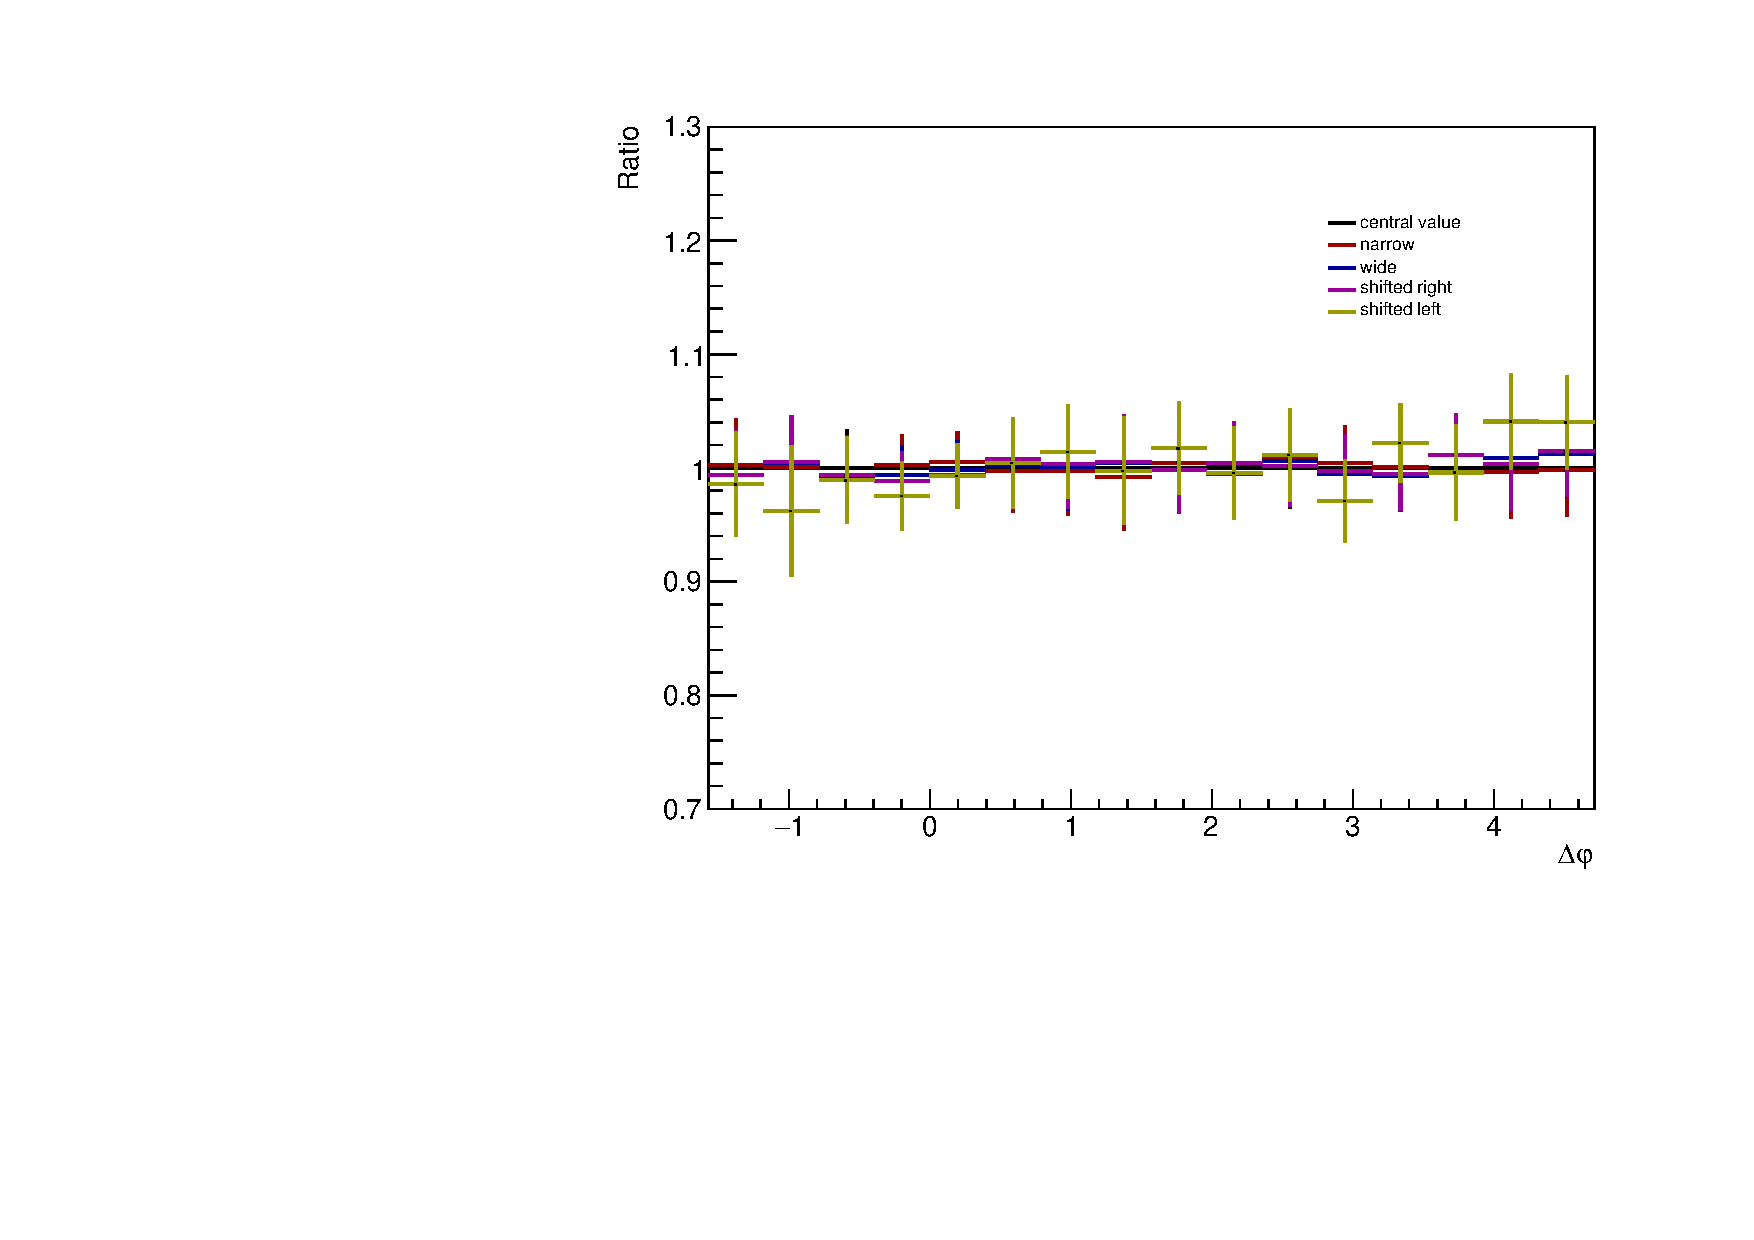
\includegraphics[width=0.49\textwidth]{figures/analysis/sideband_variations_dphi_50_80_highpt_ratio.pdf}
    \caption{The h-\lmb $\Delta\varphi$ distributions within the 0-20\% (top), 20-50\% (middle), and 50-80\% (bottom) multiplicity bins in the higher associated \pt bin for each of the sideband region variations (left) with the ratios to the nominal distribution (right).}
    \label{fig:sideband_region_variations_highpt}
\end{figure}

\subsubsection{\lmb daughter particle identification}
The \lmb daughter particle identification (PID) cuts are chosen to be wide enough to ensure a high efficiency, but narrow enough to ensure a high purity. As the requirement for a higher purity should be offset by the subtraction of the combinatorial background, altering the PID cuts should only minimally affect the final $\Delta\varphi$ distributions. To study this, the PID cuts are varied in the ways presented in Table~\ref{tab:pid_cut_variations}. The final $\Delta\varphi$ distributions and ratios to the nominal distribution for each PID cut variation in each multiplicity and associated \pt bin are shown in Figures \ref{fig:pid_cut_variations_lowpt} (lower \pt) and \ref{fig:pid_cut_variations_highpt} (higher \pt). Requiring a signal in the TOF detector drastically reduces the $\Lambda$ signal as the daugher pions are often heavily deflected by the magnetic field due to their lower \pt (again, $m_{\text{p}}/m_{\pi} \approx 7$, so most of the mother momentum belongs to the proton). This causes a large amount of statistical fluctuations in the corresponding $\Delta\varphi$ distribution, which is why the ``require TOF'' variation is inevitably excluded after the Barlow check presented in Section~\ref{sec:barlow_check_dphi}. The other variations result in only around a 2\% deviation from the nominal $\Delta\varphi$ distribution, on average.

\begin{table}[ht]
    \centering
    \caption{The variations of the \lmb daughter PID cuts considered for this analysis. The ``require TOF'' variation requires a TOF hit for both the proton and pion, but maintains the nominal values for $|n\sigma_{\text{TPC, TOF}}|$.}
    \label{tab:pid_cut_variations}
    \begin{tabular}{l c c}
        \hline
        Variation name & $|n\sigma_{\text{TPC}, \text{TOF}}^{\pi}|$ & $|n\sigma_{\text{TPC}, \text{TOF}}^{\text{p}}|$ \\
        \hline
        Narrow & $< 1.8$ & $< 1.2$ \\
        Wide & $< 4.2$ & $< 2.8$ \\
        Require TOF & $< 3.0$ & $< 2.0$ \\
        \hline
    \end{tabular}
\end{table}

\begin{figure}[ht]
    \centering
    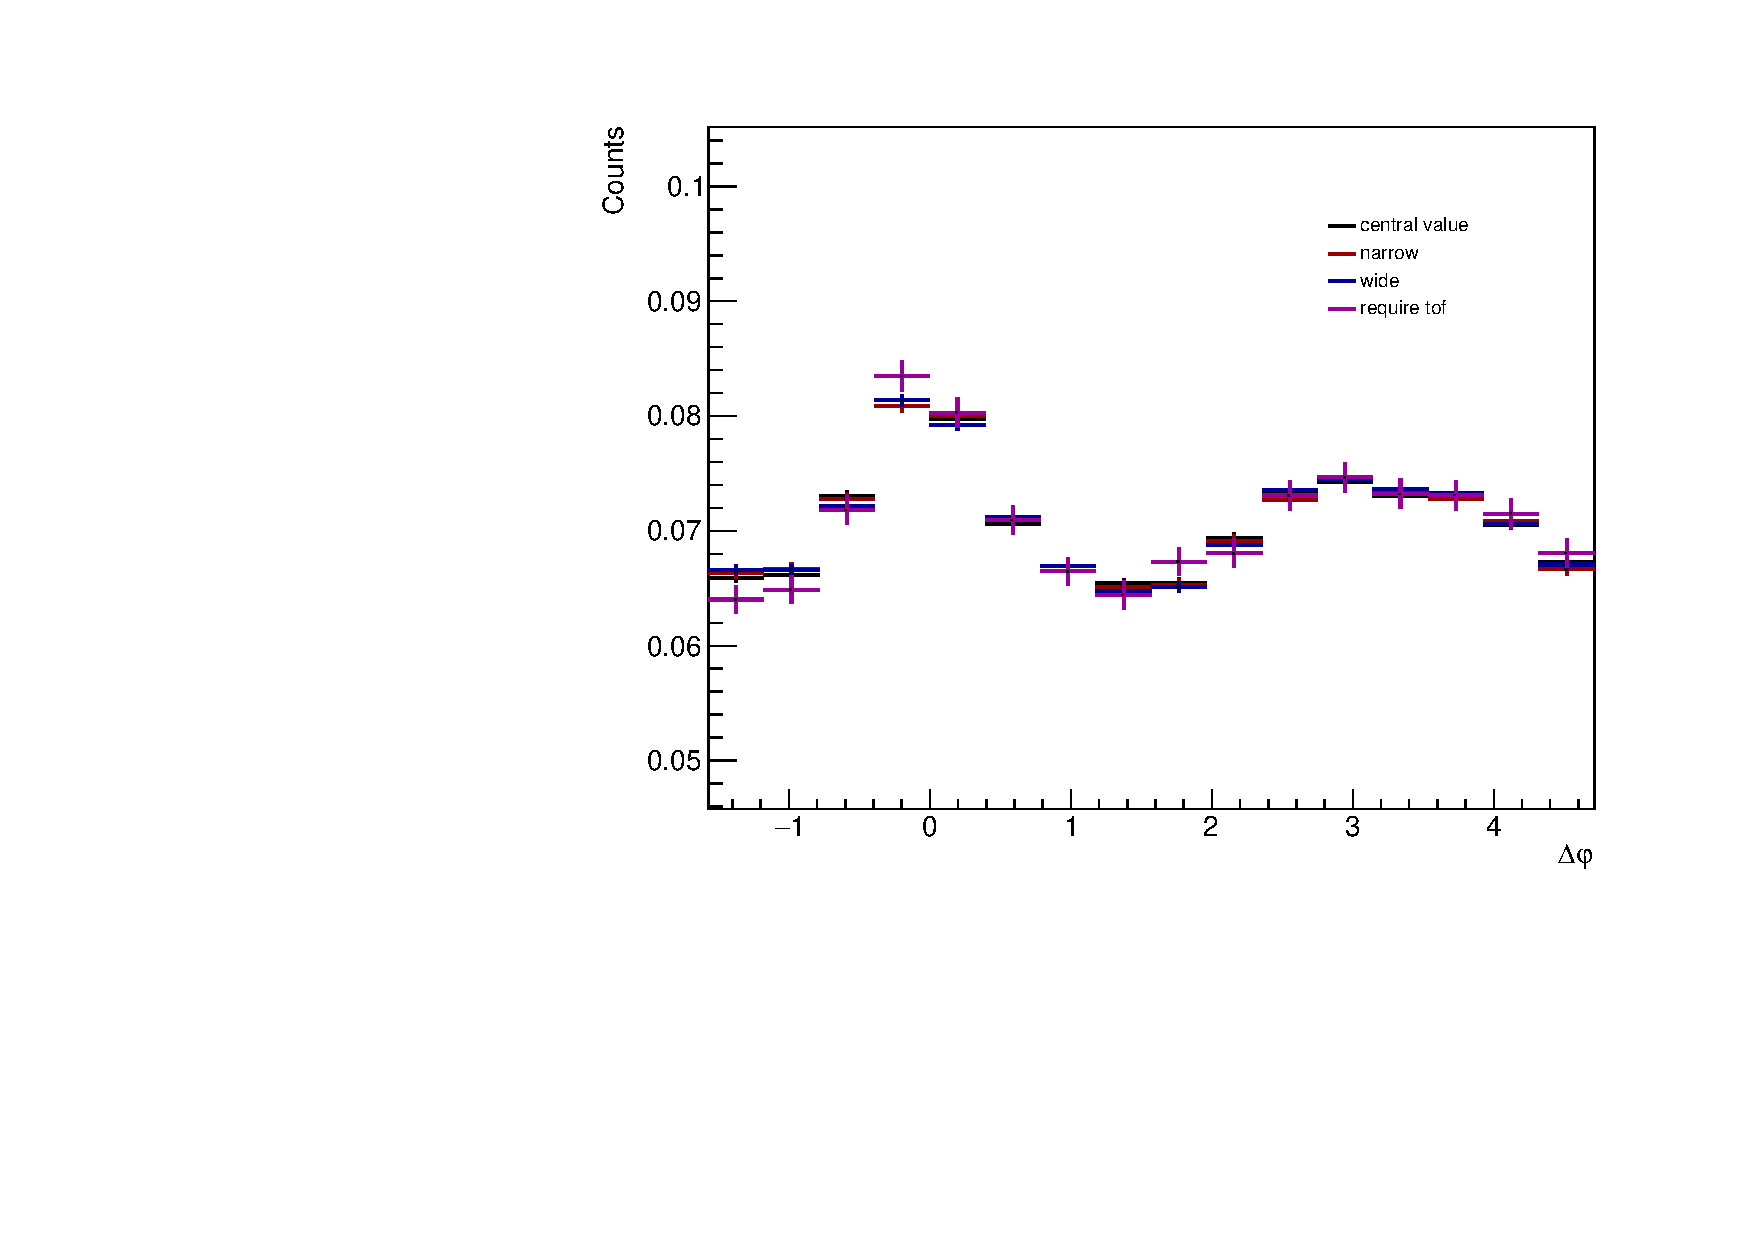
\includegraphics[width=0.49\textwidth]{figures/analysis/pid_variations_dphi_0_20_lowpt.pdf}
    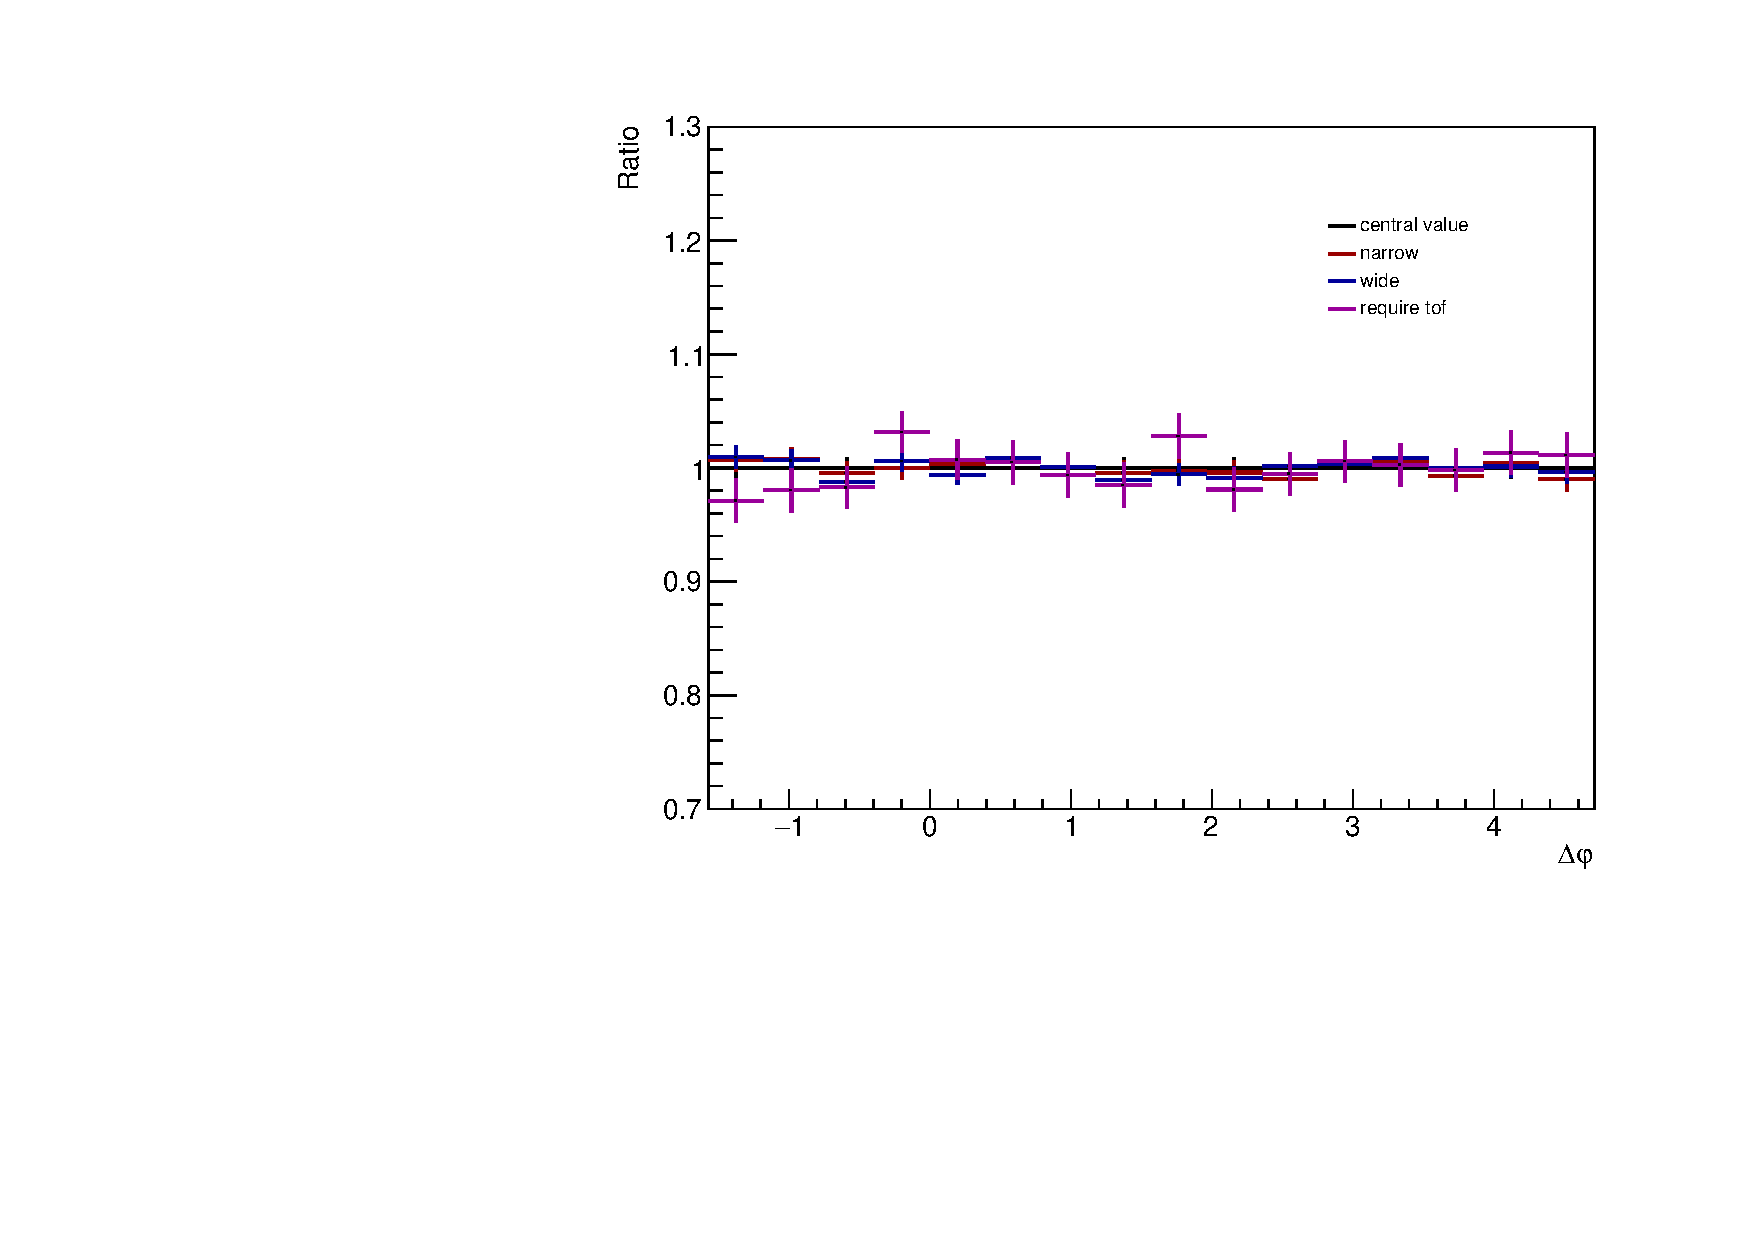
\includegraphics[width=0.49\textwidth]{figures/analysis/pid_variations_dphi_0_20_lowpt_ratio.pdf}
    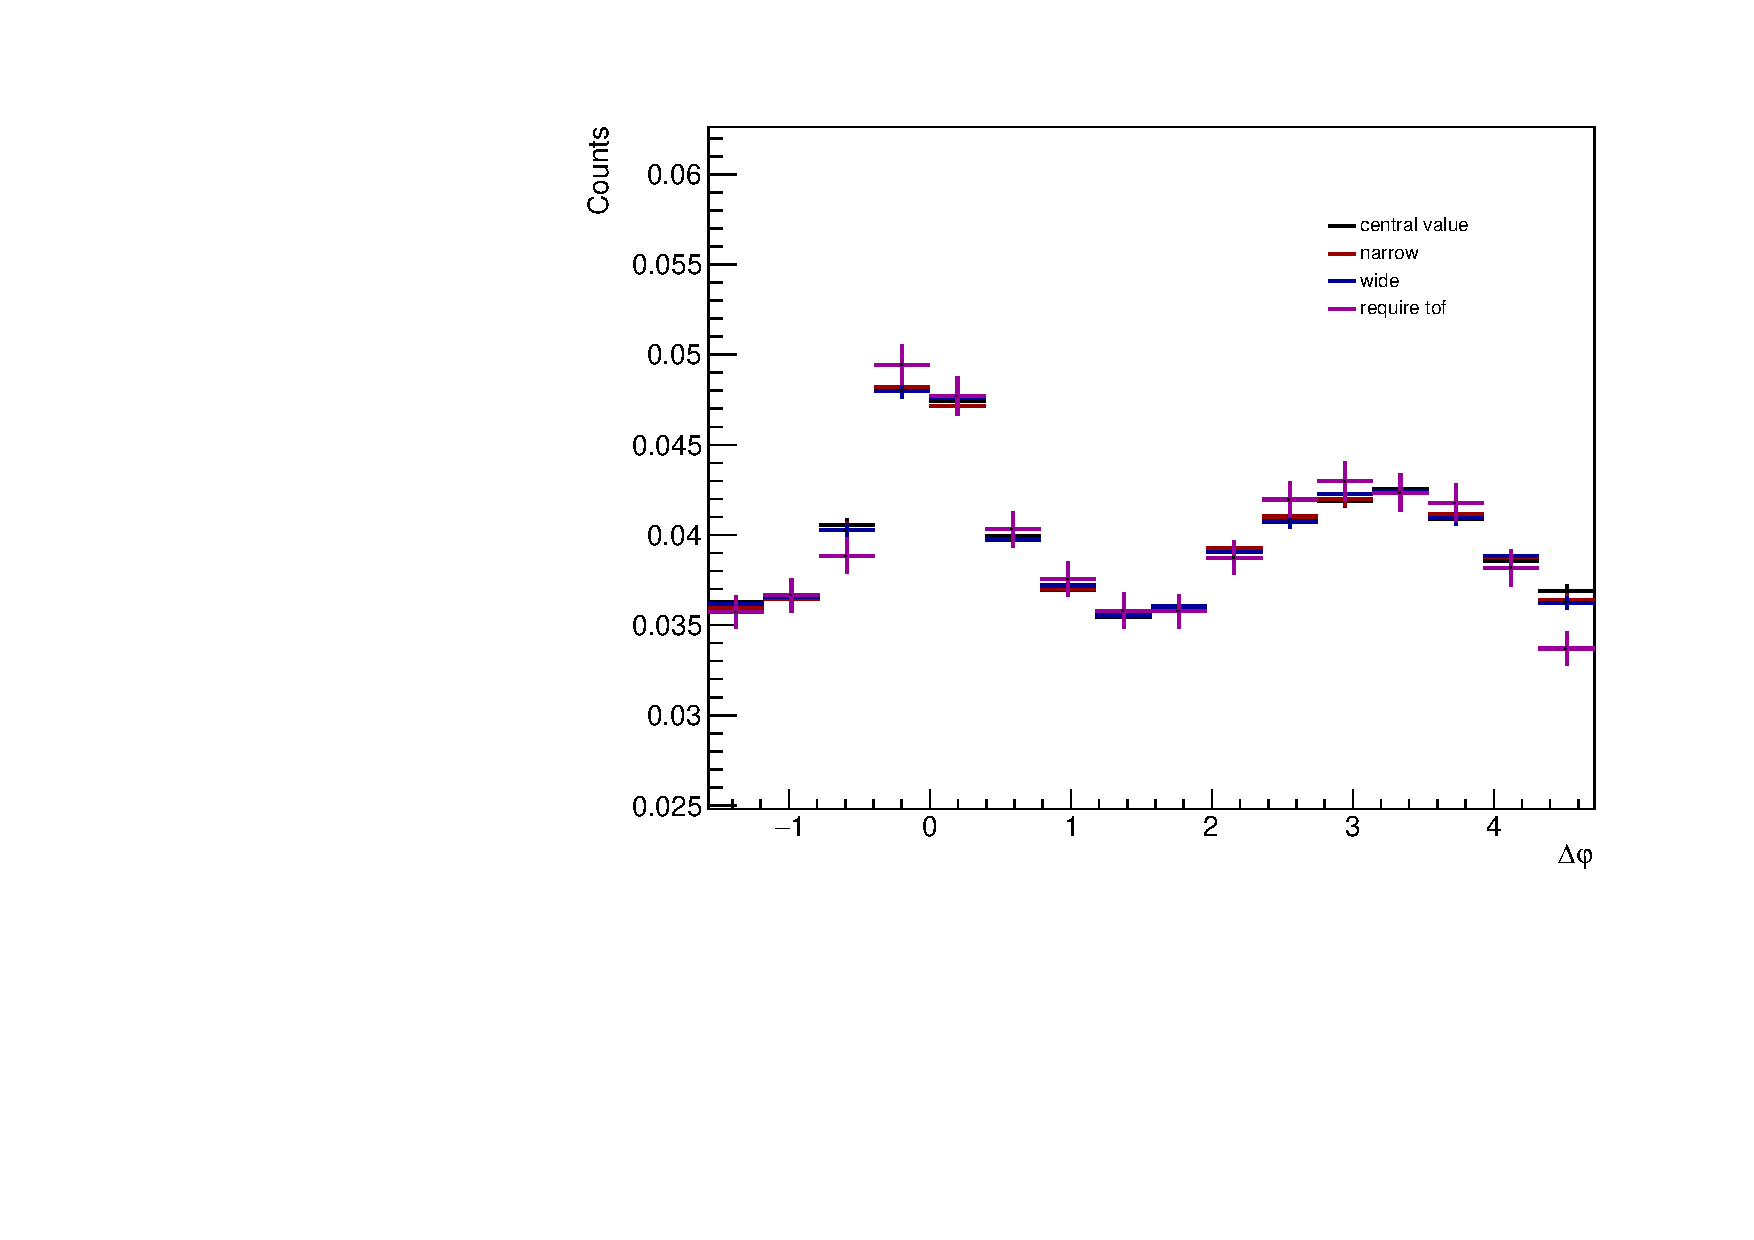
\includegraphics[width=0.49\textwidth]{figures/analysis/pid_variations_dphi_20_50_lowpt.pdf}
    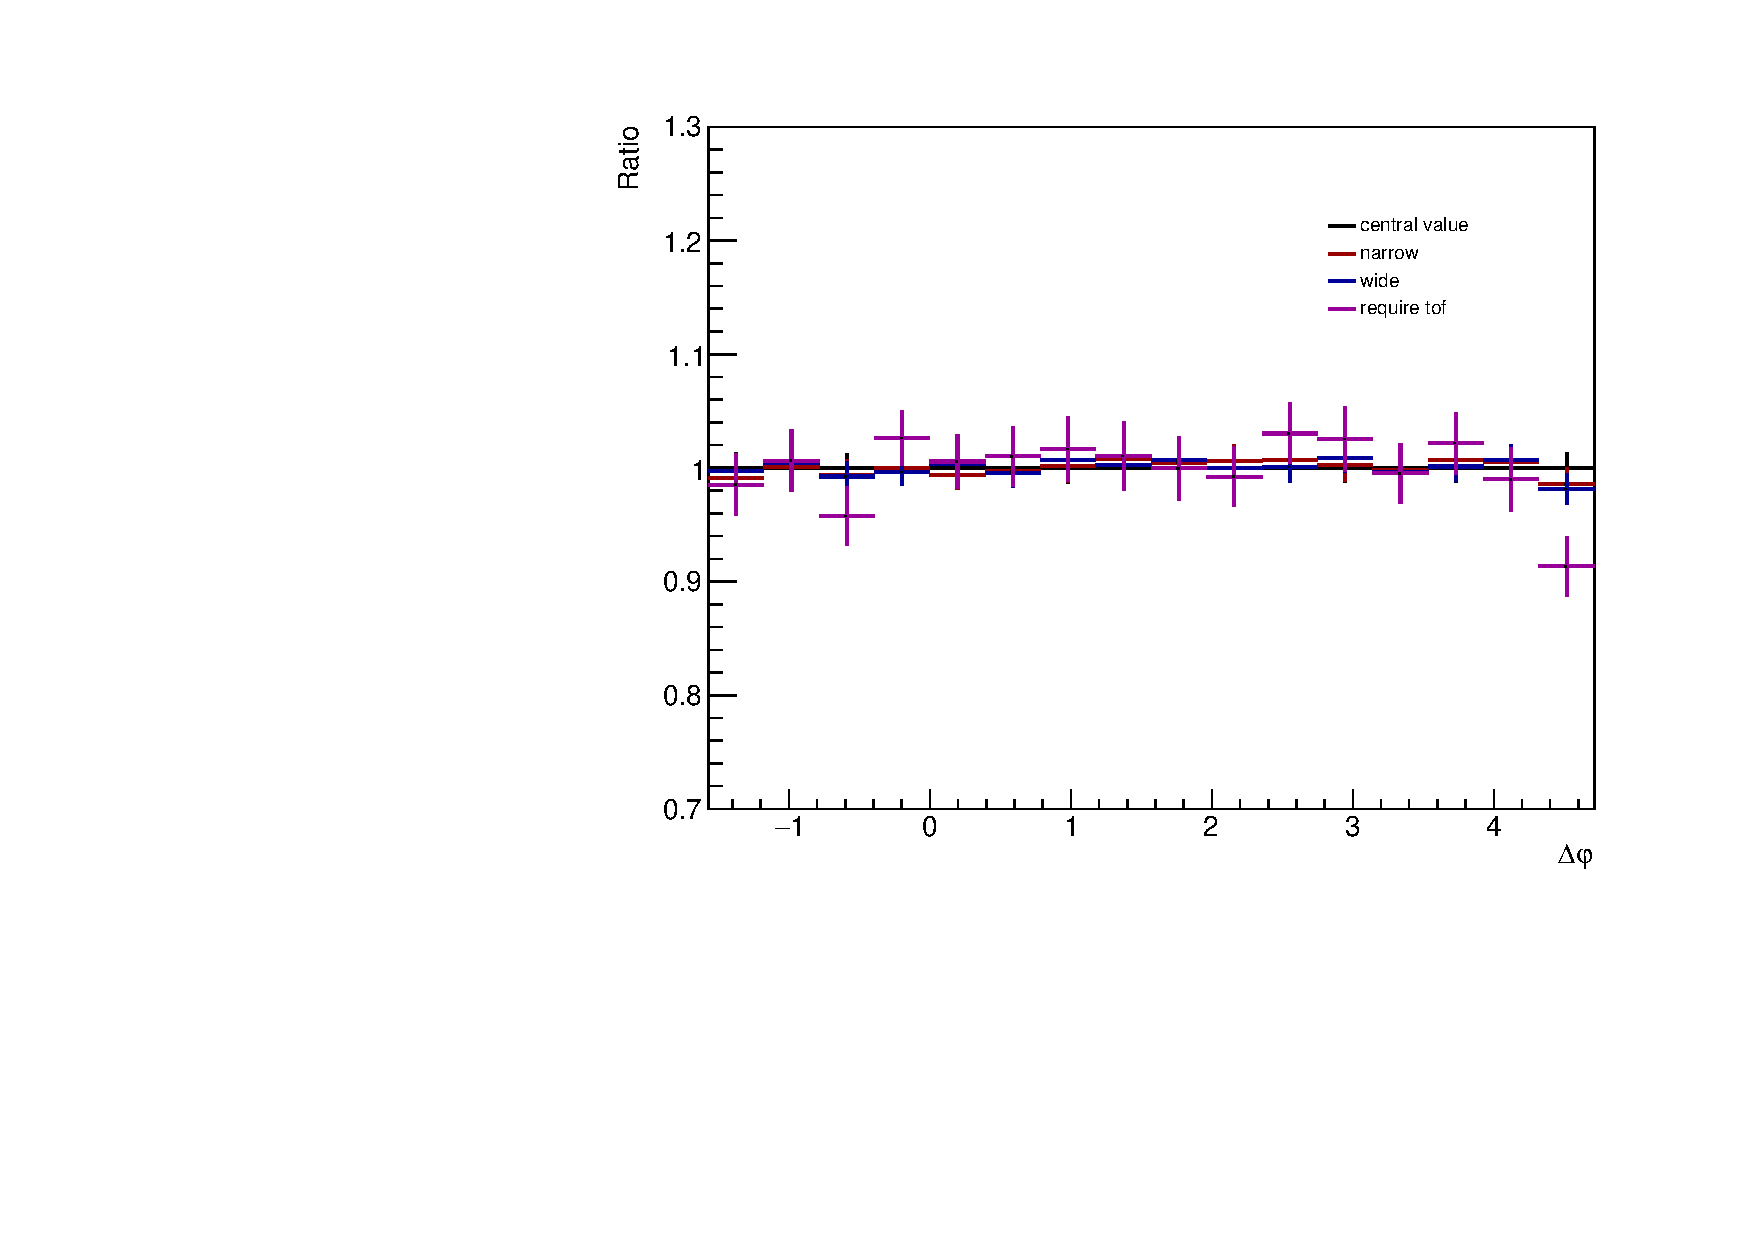
\includegraphics[width=0.49\textwidth]{figures/analysis/pid_variations_dphi_20_50_lowpt_ratio.pdf}
    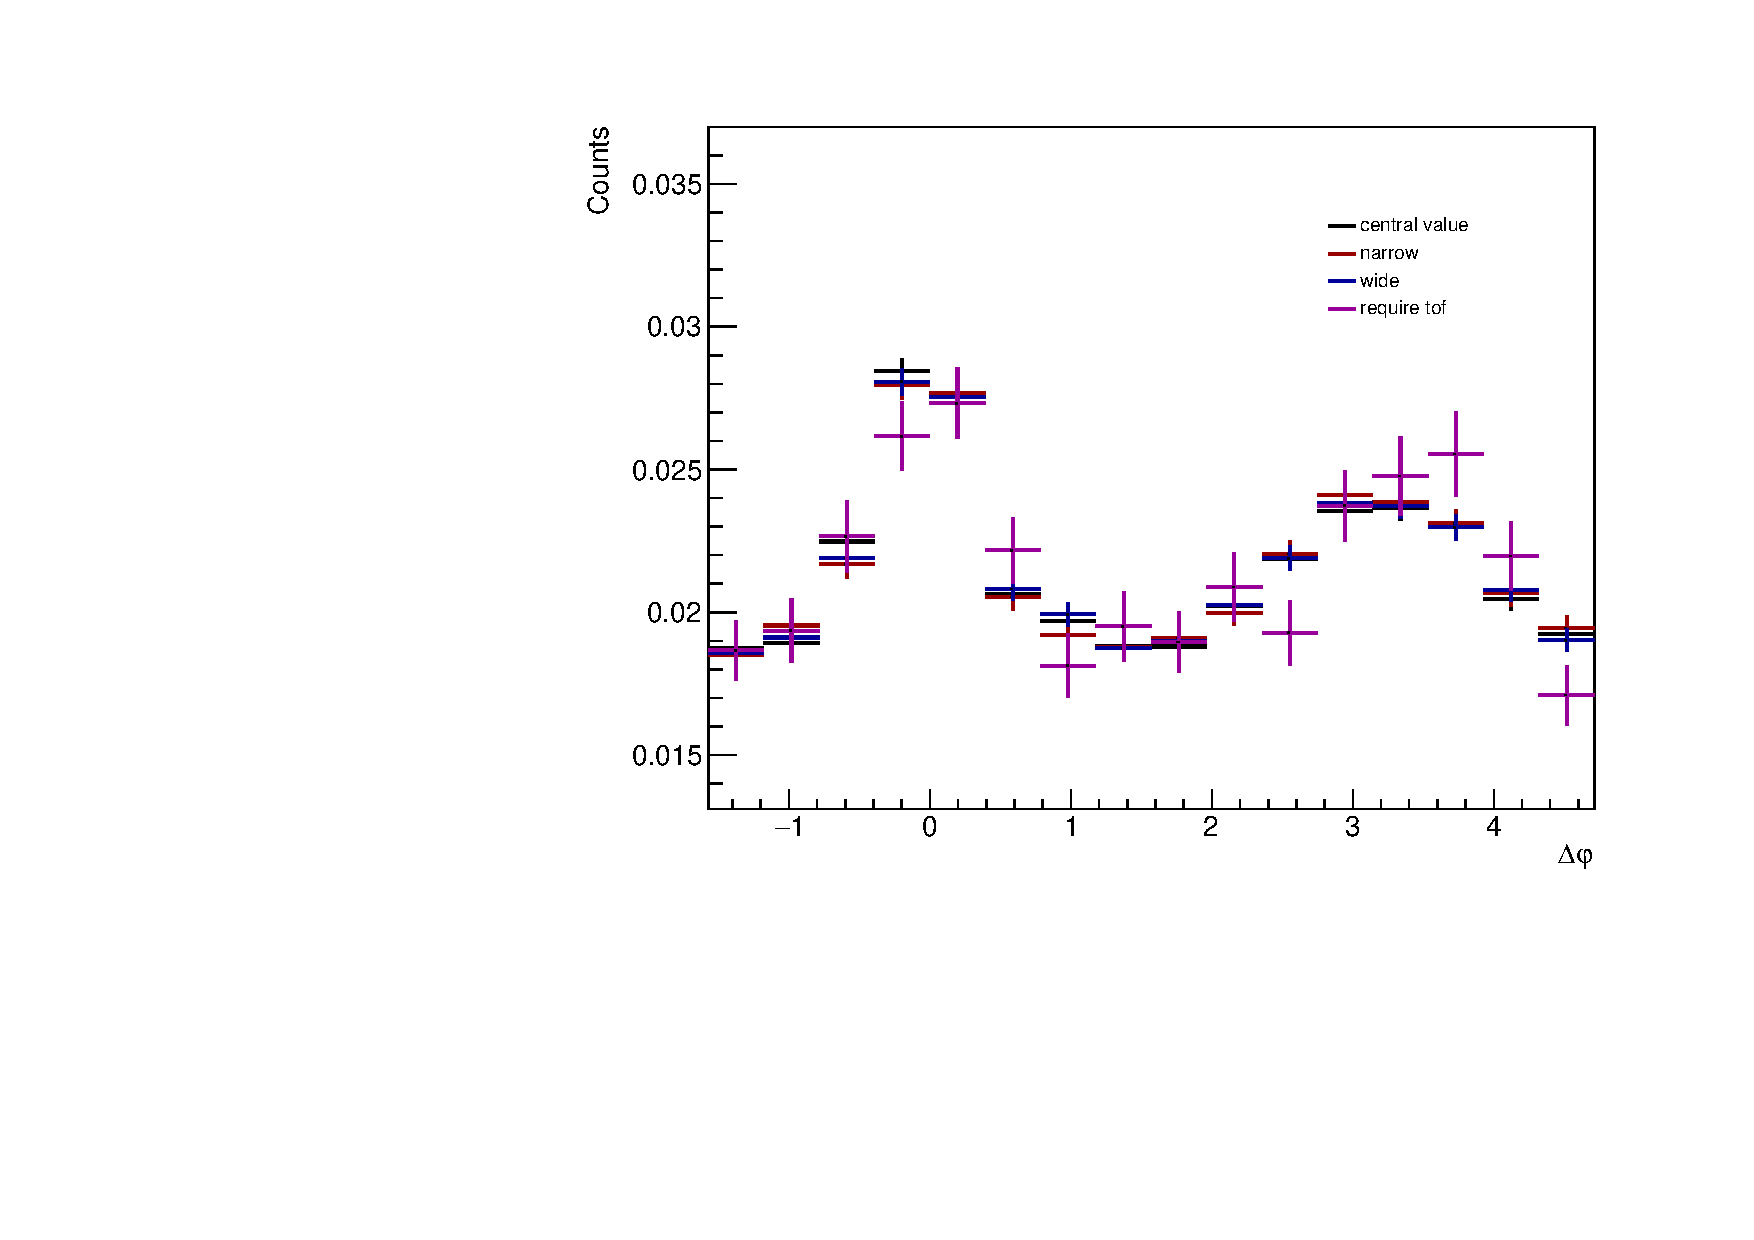
\includegraphics[width=0.49\textwidth]{figures/analysis/pid_variations_dphi_50_80_lowpt.pdf}
    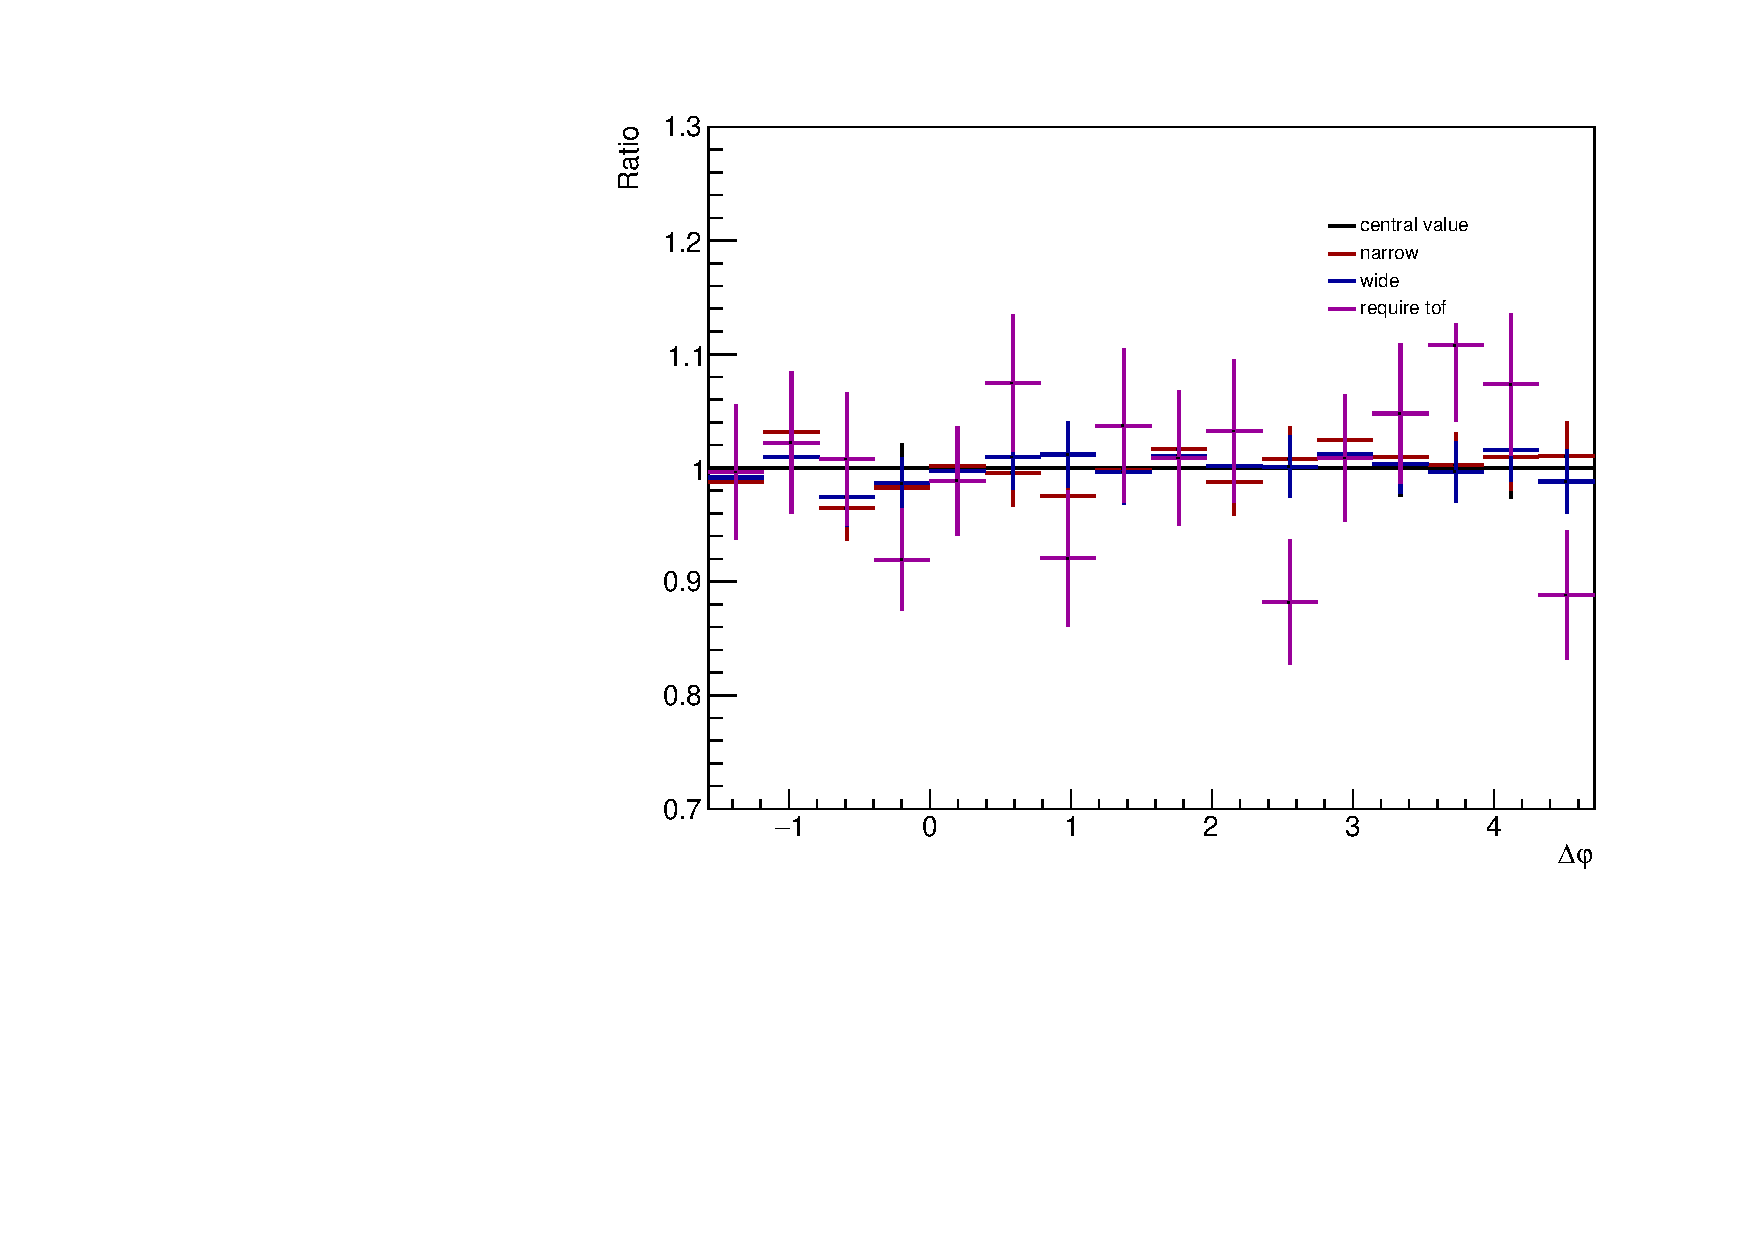
\includegraphics[width=0.49\textwidth]{figures/analysis/pid_variations_dphi_50_80_lowpt_ratio.pdf}
    \caption{The h-\lmb $\Delta\varphi$ distributions within the 0-20\% (top), 20-50\% (middle), and 50-80\% (bottom) multiplicity bins in the lower associated \pt bin for each of the PID cut variations (left) with the ratios to the nominal distribution (right).}
    \label{fig:pid_cut_variations_lowpt}
\end{figure}

\begin{figure}[ht]
    \centering
    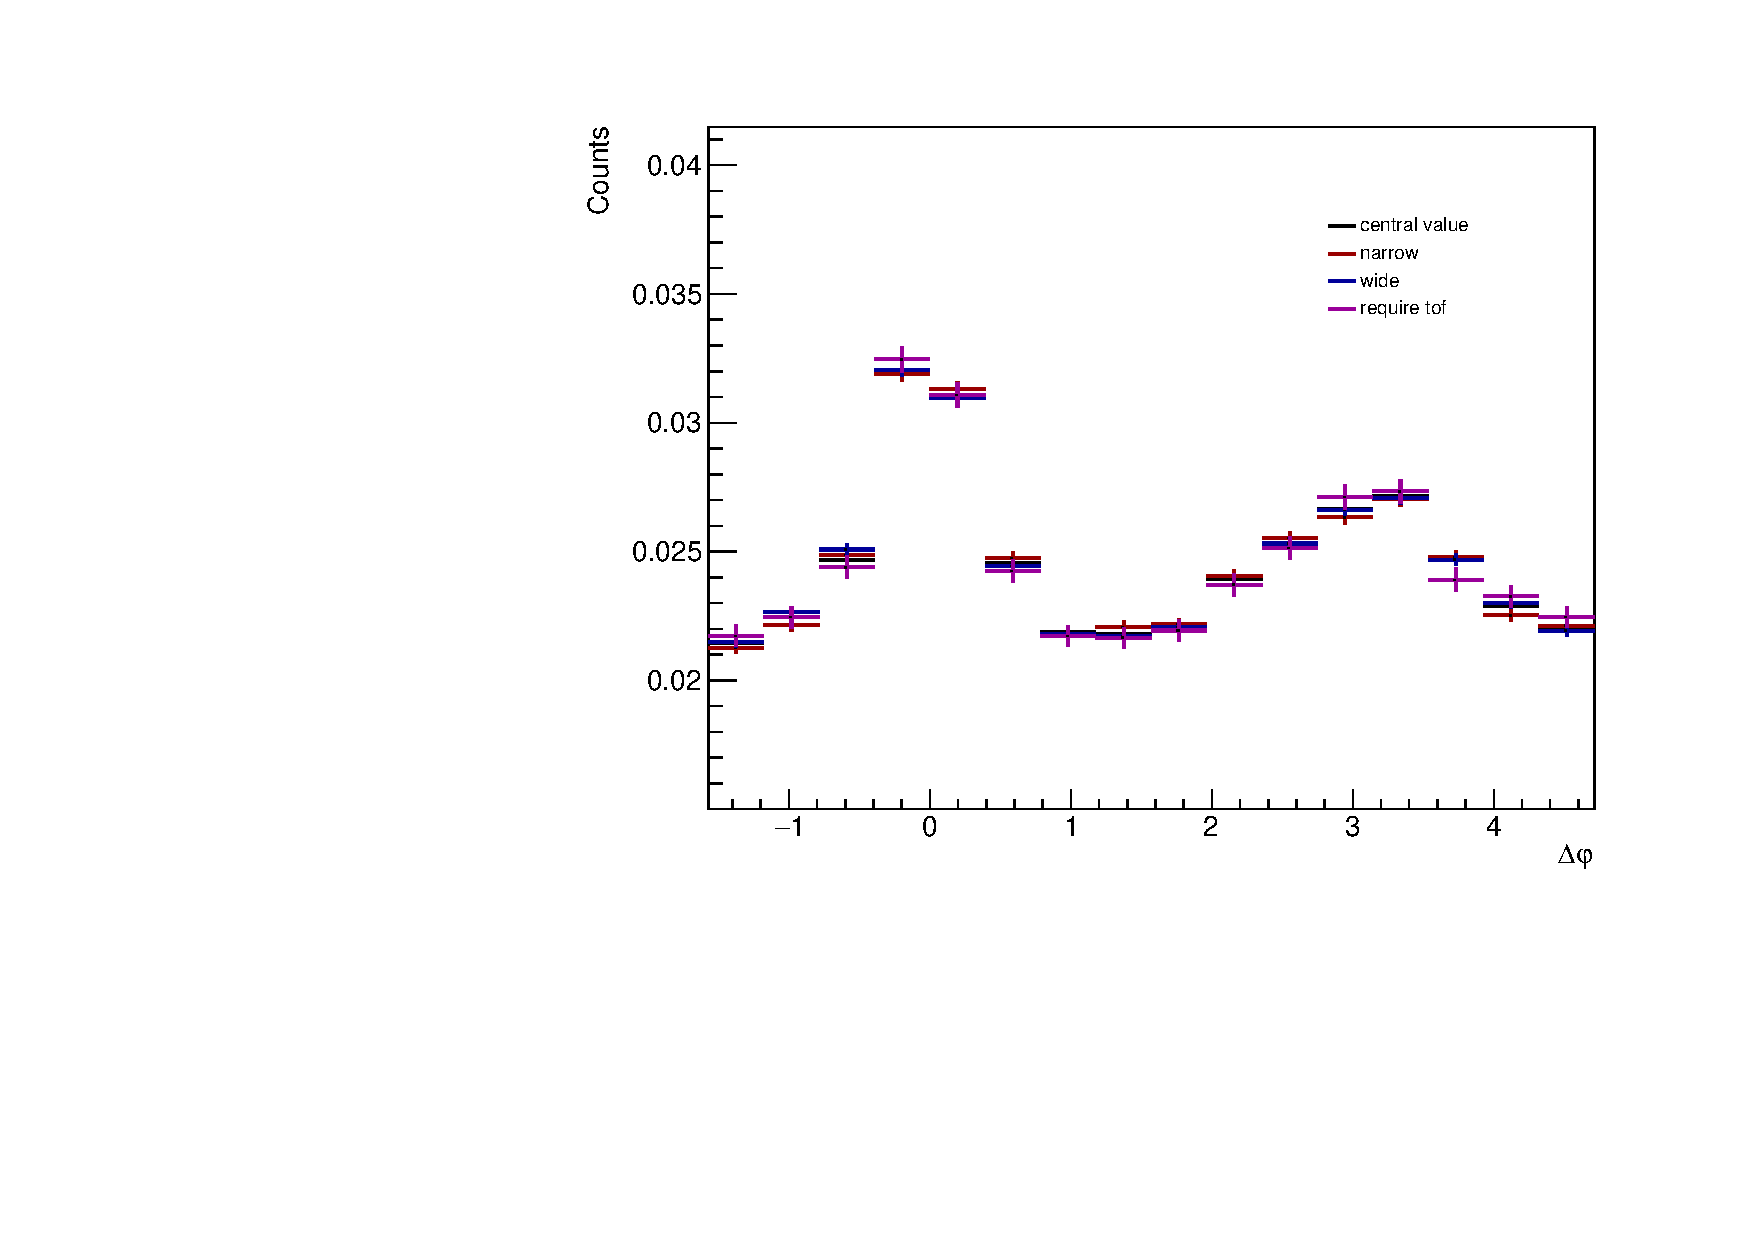
\includegraphics[width=0.49\textwidth]{figures/analysis/pid_variations_dphi_0_20_highpt.pdf}
    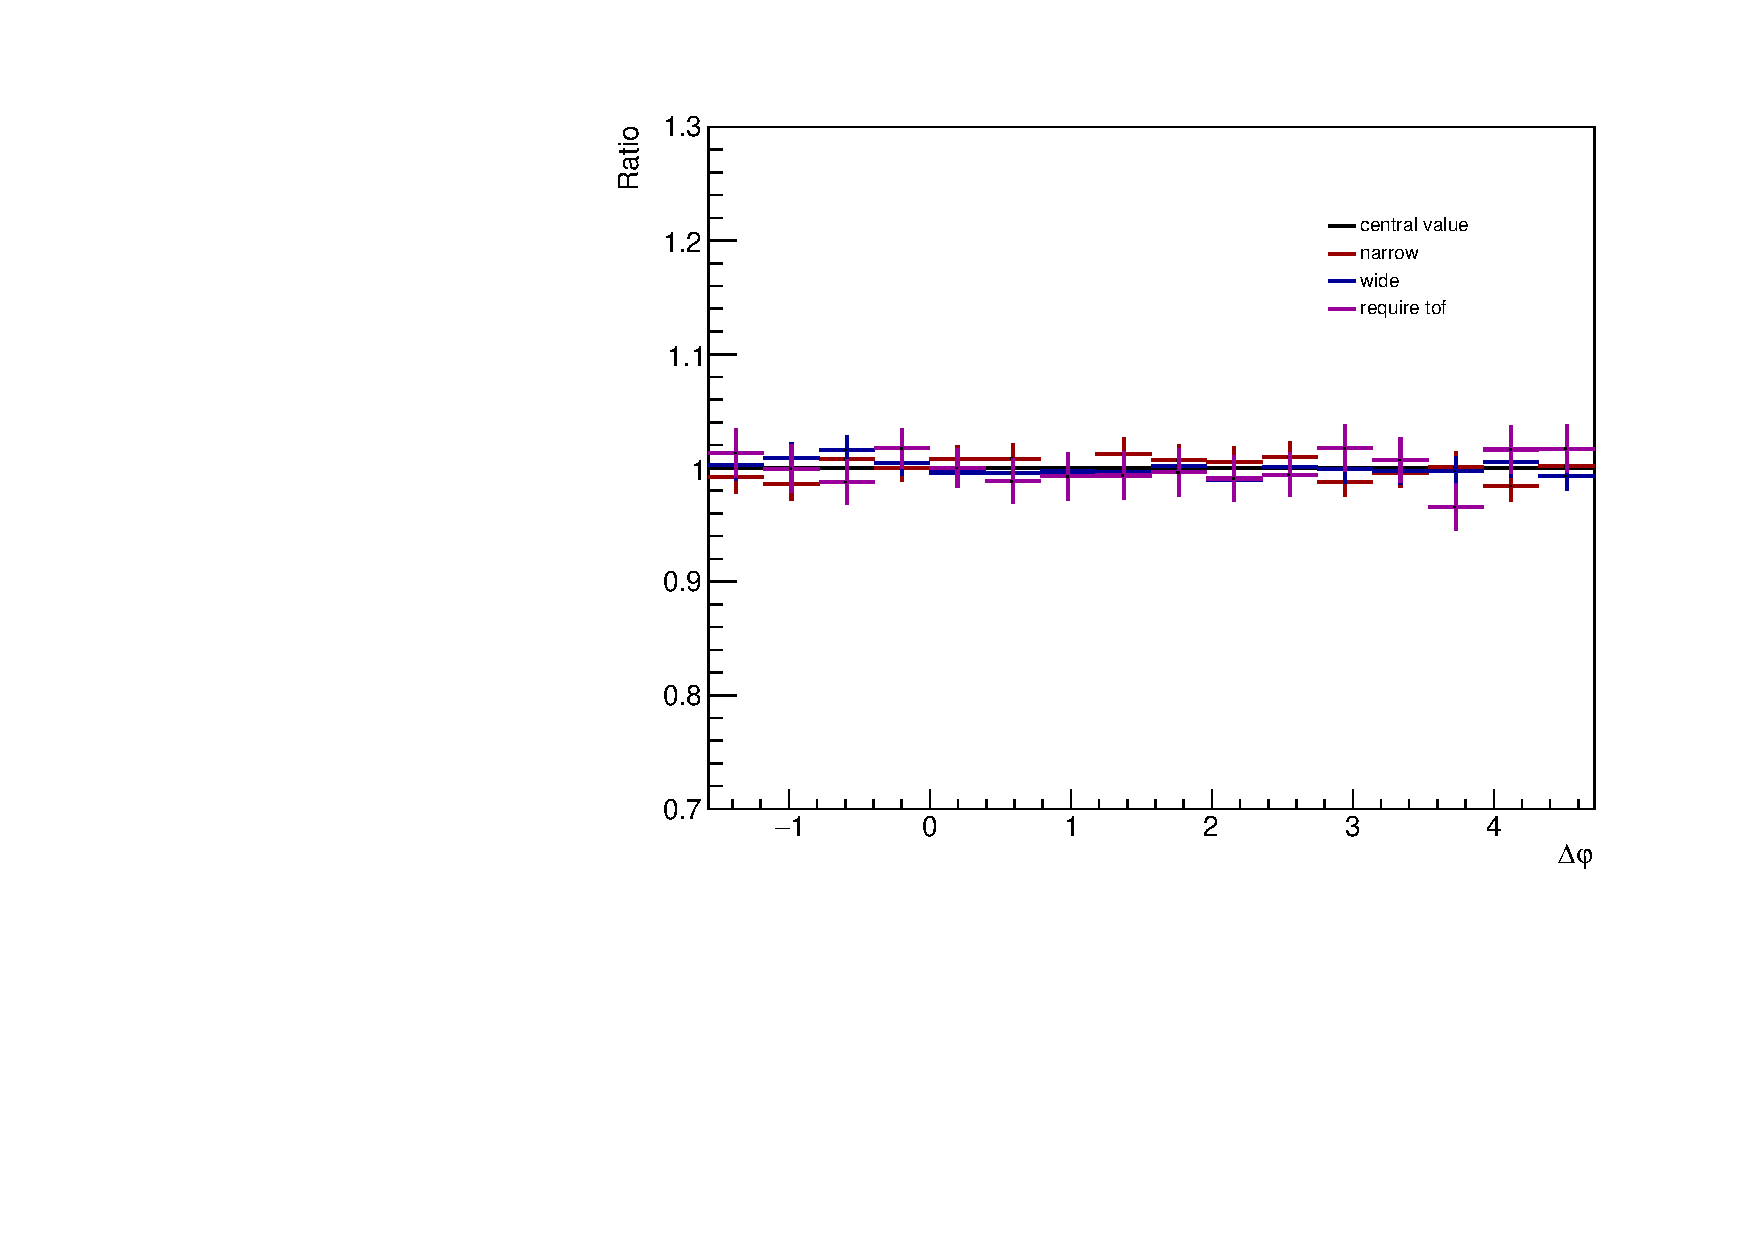
\includegraphics[width=0.49\textwidth]{figures/analysis/pid_variations_dphi_0_20_highpt_ratio.pdf}
    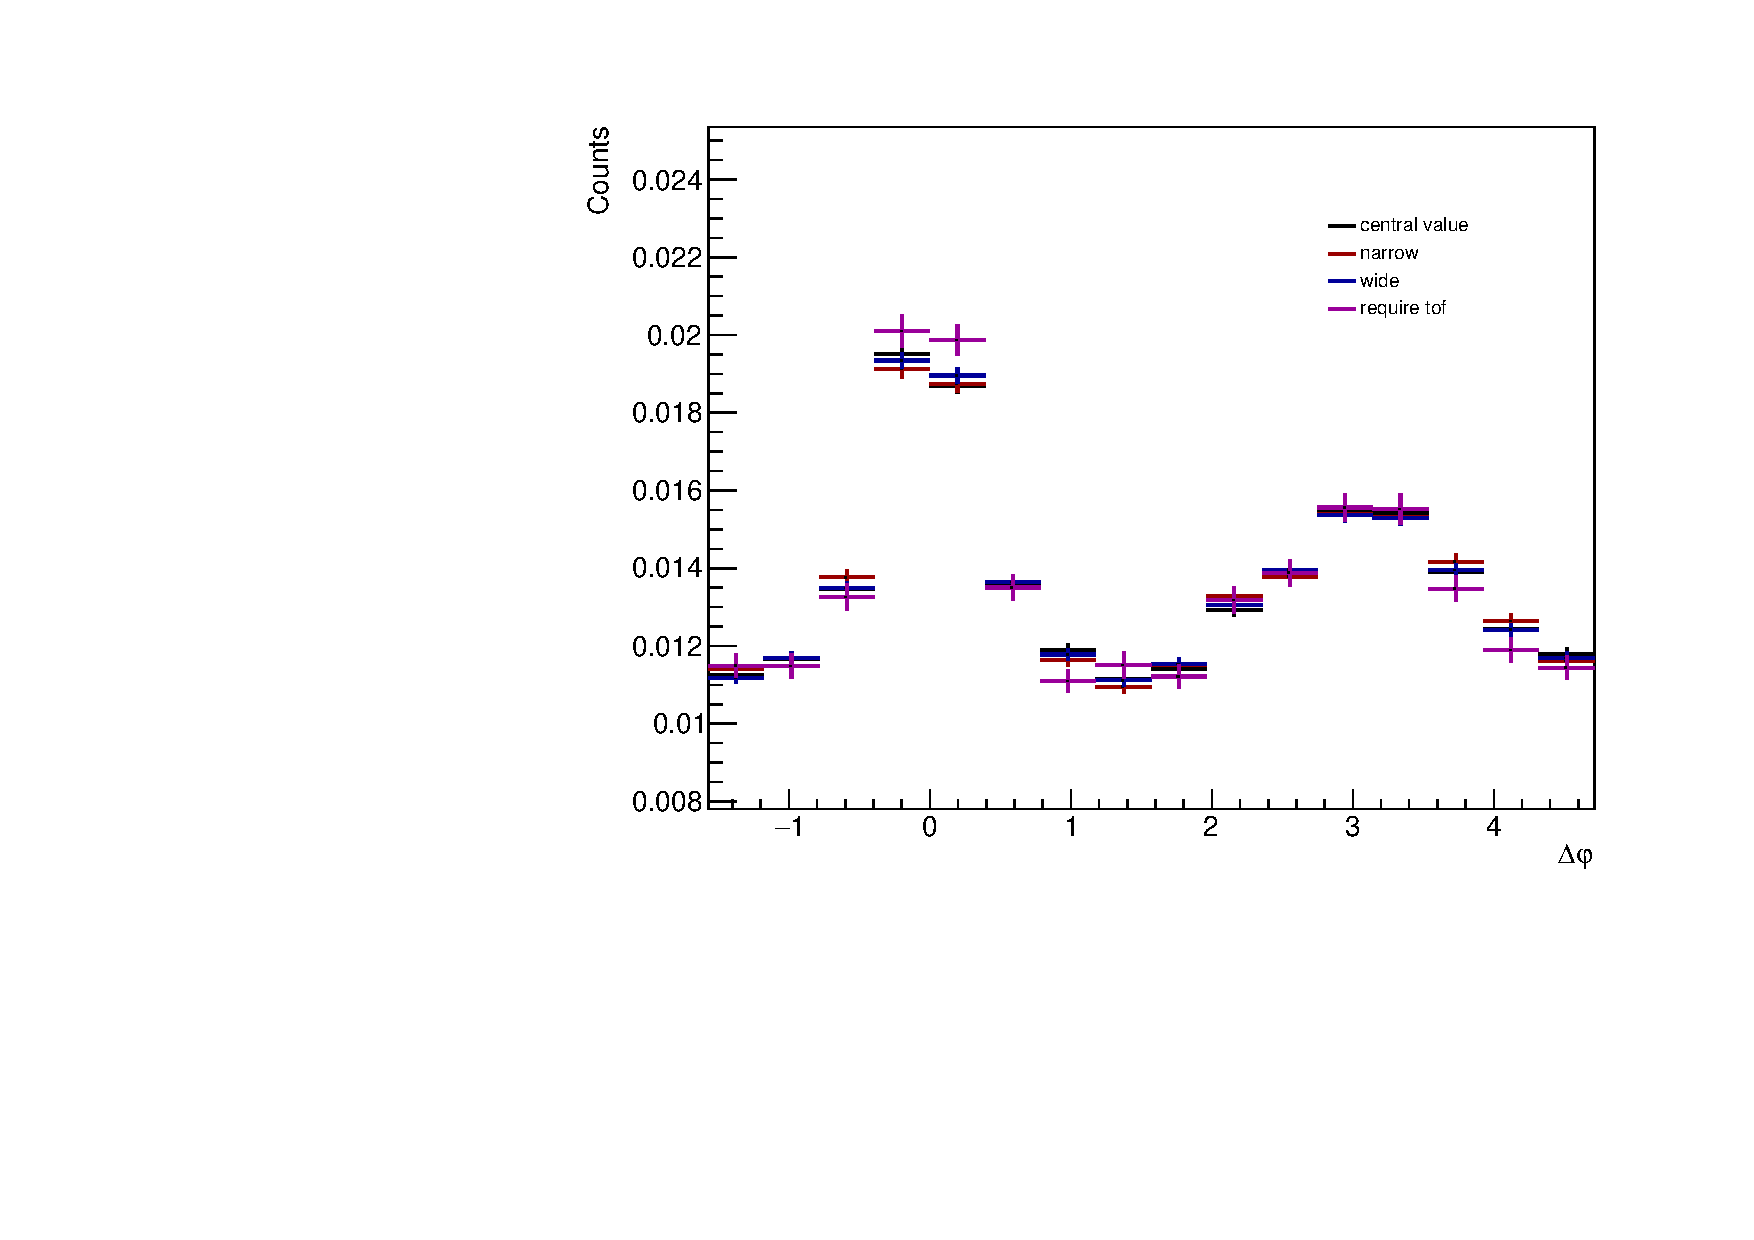
\includegraphics[width=0.49\textwidth]{figures/analysis/pid_variations_dphi_20_50_highpt.pdf}
    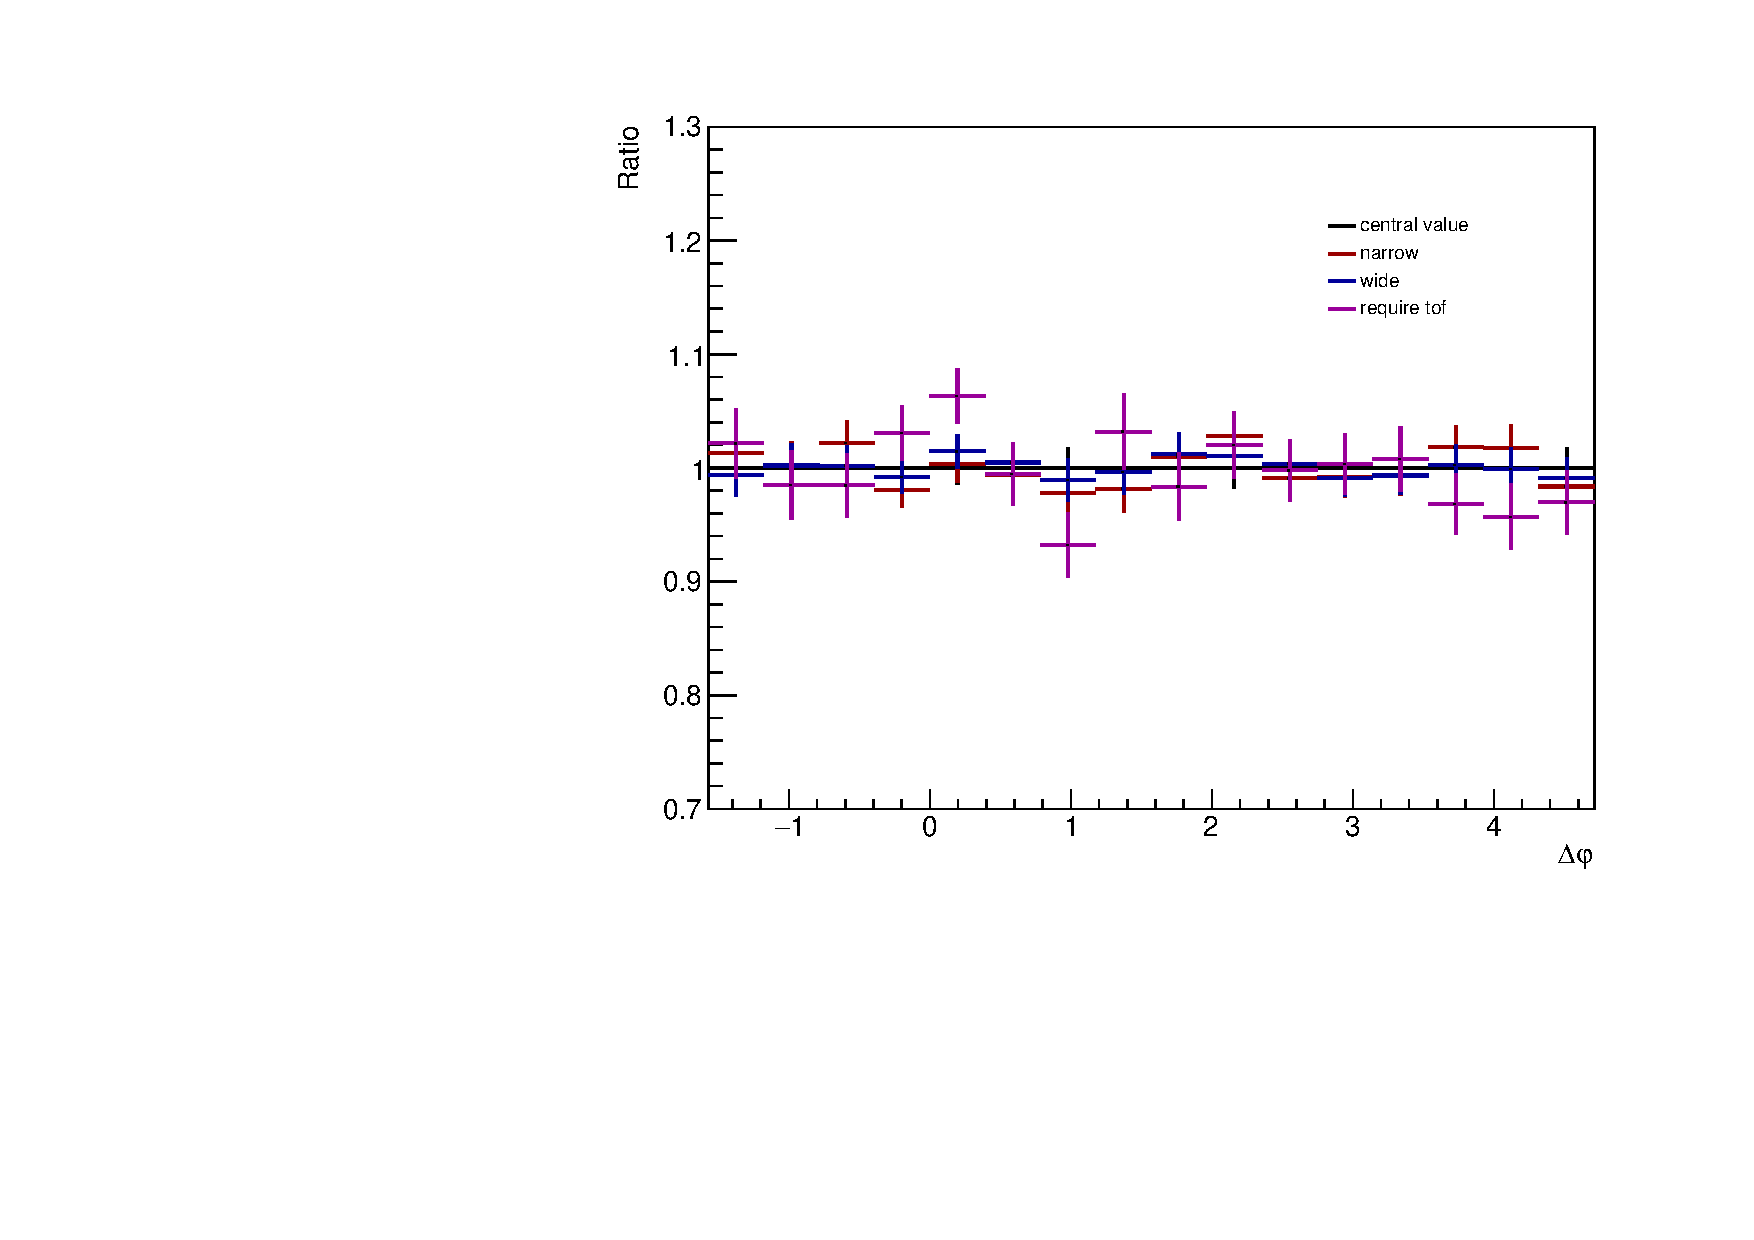
\includegraphics[width=0.49\textwidth]{figures/analysis/pid_variations_dphi_20_50_highpt_ratio.pdf}
    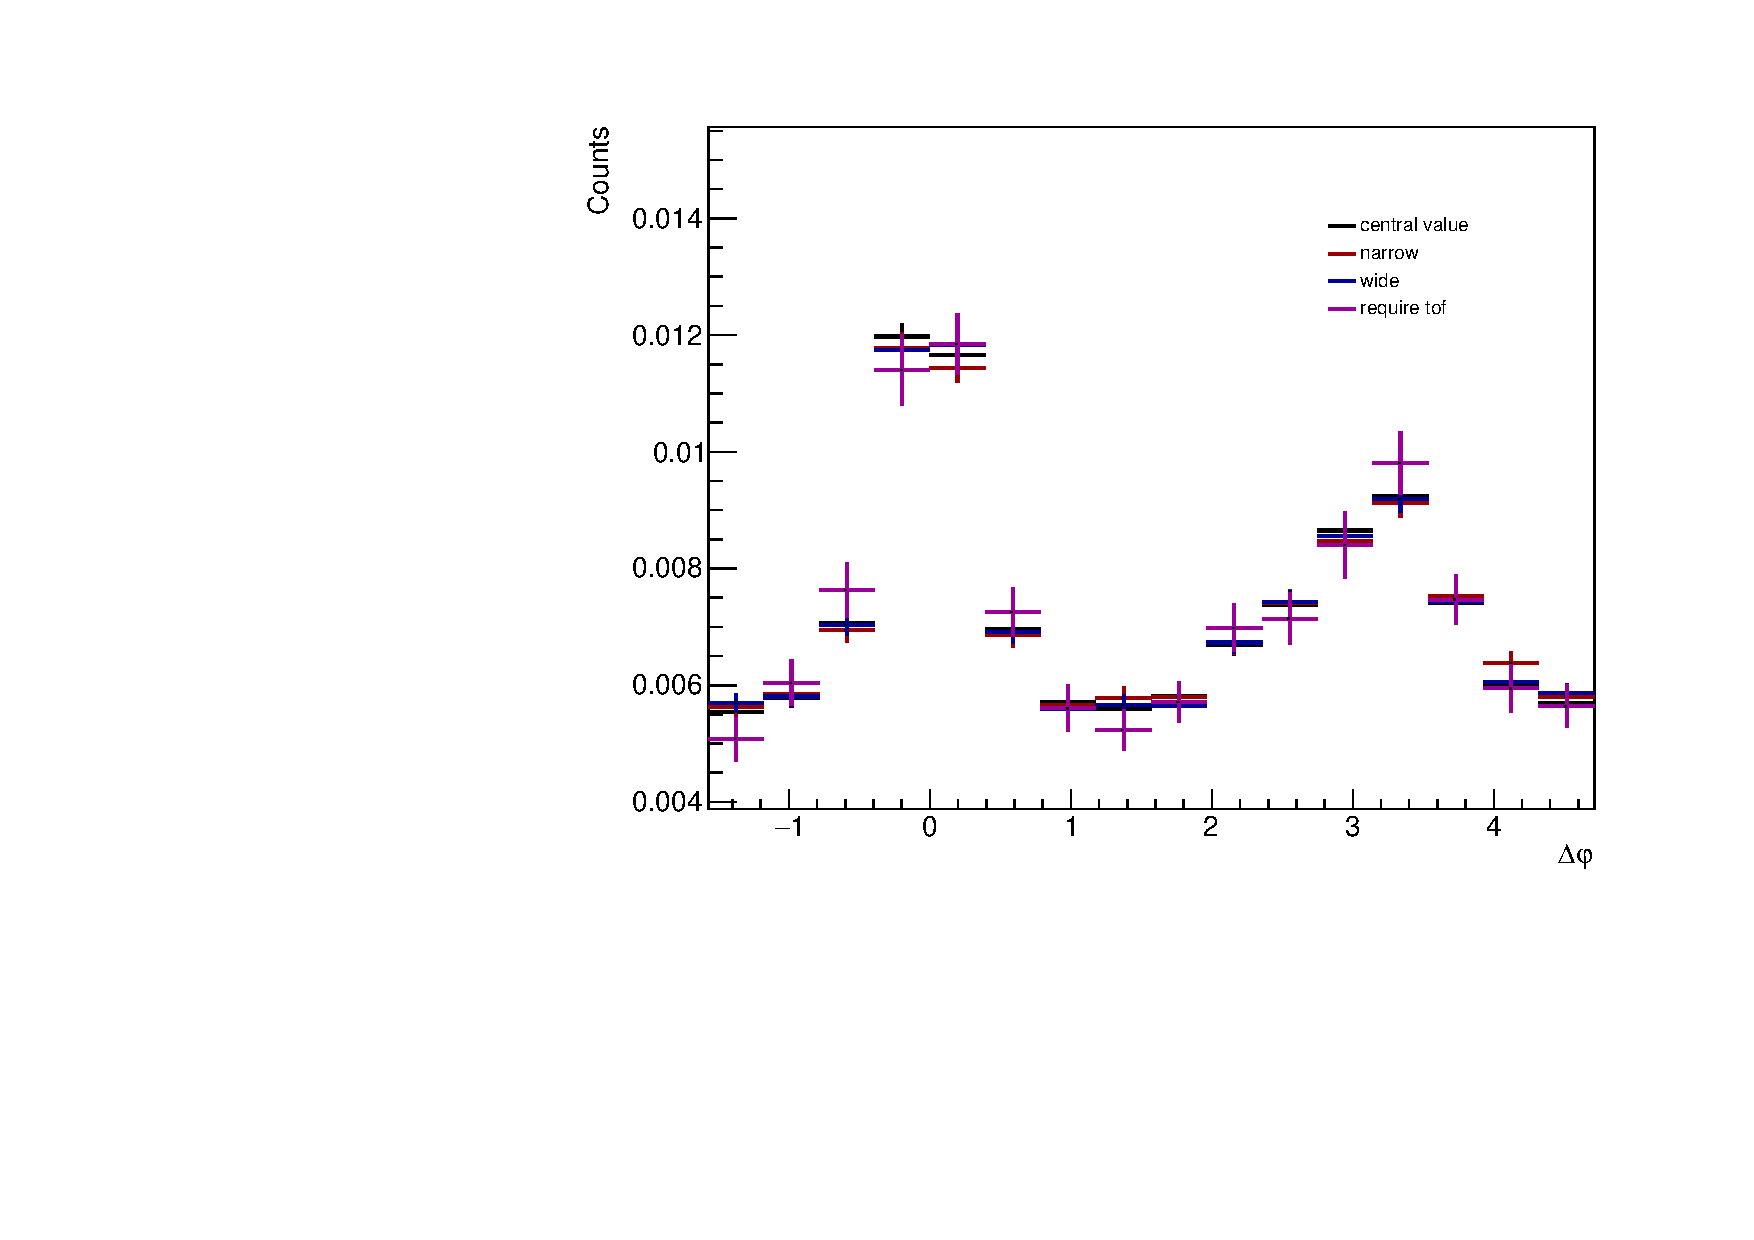
\includegraphics[width=0.49\textwidth]{figures/analysis/pid_variations_dphi_50_80_highpt.pdf}
    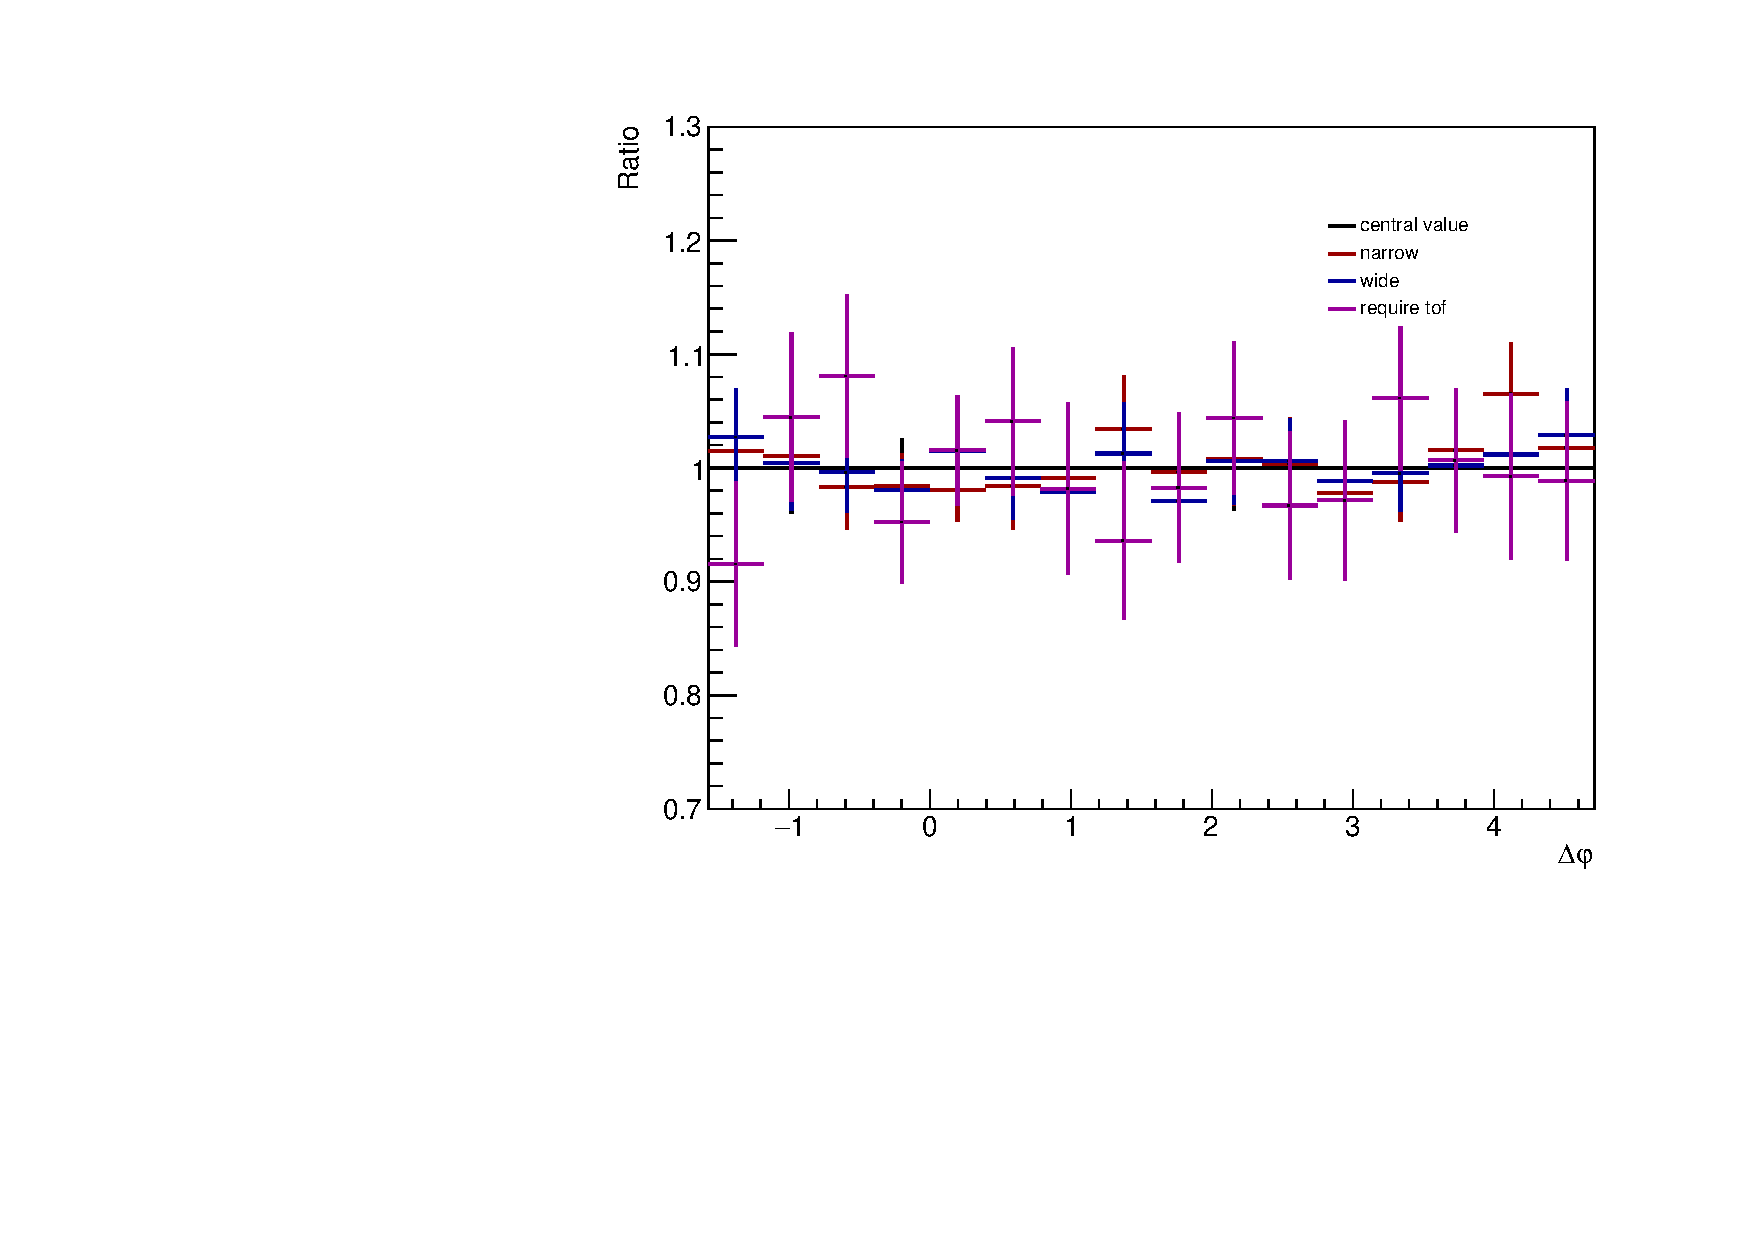
\includegraphics[width=0.49\textwidth]{figures/analysis/pid_variations_dphi_50_80_highpt_ratio.pdf}
    \caption{The h-\lmb $\Delta\varphi$ distributions within the 0-20\% (top), 20-50\% (middle), and 50-80\% (bottom) multiplicity bins in the higher associated \pt bin for each of the PID cut variations (left) with the ratios to the nominal distribution (right).}
    \label{fig:pid_cut_variations_highpt}
\end{figure}

\clearpage

\subsubsection{Barlow check for $\Delta\varphi$ distribution generation}
\label{sec:barlow_check_dphi}

Due to statistical fluctuations, it may be the case that some variations result in a statistically insignificant deviation from the nominal $\Delta\varphi$ distribution. In such cases, the variation should not be considered in the final systematic uncertainty calculation. To determine which variations give statistically significant deviations, a Barlow check~\cite{BarlowCheck} is performed. For each $\Delta\varphi$ bin, the following quantity is calculated:
%
\begin{equation}
    \label{eq:barlow_check}
	N\sigma_{RB} := \frac{y_{\text{var.}} - y_{\text{nom.}}}{\sqrt{|\sigma_{\text{var.}}^2 - \sigma_{\text{nom.}}^2|}},
\end{equation}
%
where $y_{\text{var.}}$ and $\sigma_{\text{var.}}$ are the measured yield and statistical uncertainty for the variation, and $y_{\text{nom.}}$ and $\sigma_{\text{nom.}}$ are the yield and statistical uncertainty for the nominal value. 

To determine whether a given variation should be excluded, the number of $\Delta\varphi$ bins that have $|N\sigma_{RB}| < 1$ is counted. If this is the majority of the bins (across all multiplicity and associated \pt ranges), the variation is excluded from the systematic calculation. Example plots of $N\sigma_{RB}$ for each variation of the signal, sideband and PID cuts are shown in Figure \ref{fig:barlow_check_0_20}. The red lines represent $N\sigma_{RB} = \pm 1$.

\begin{figure}[ht]
    \centering
    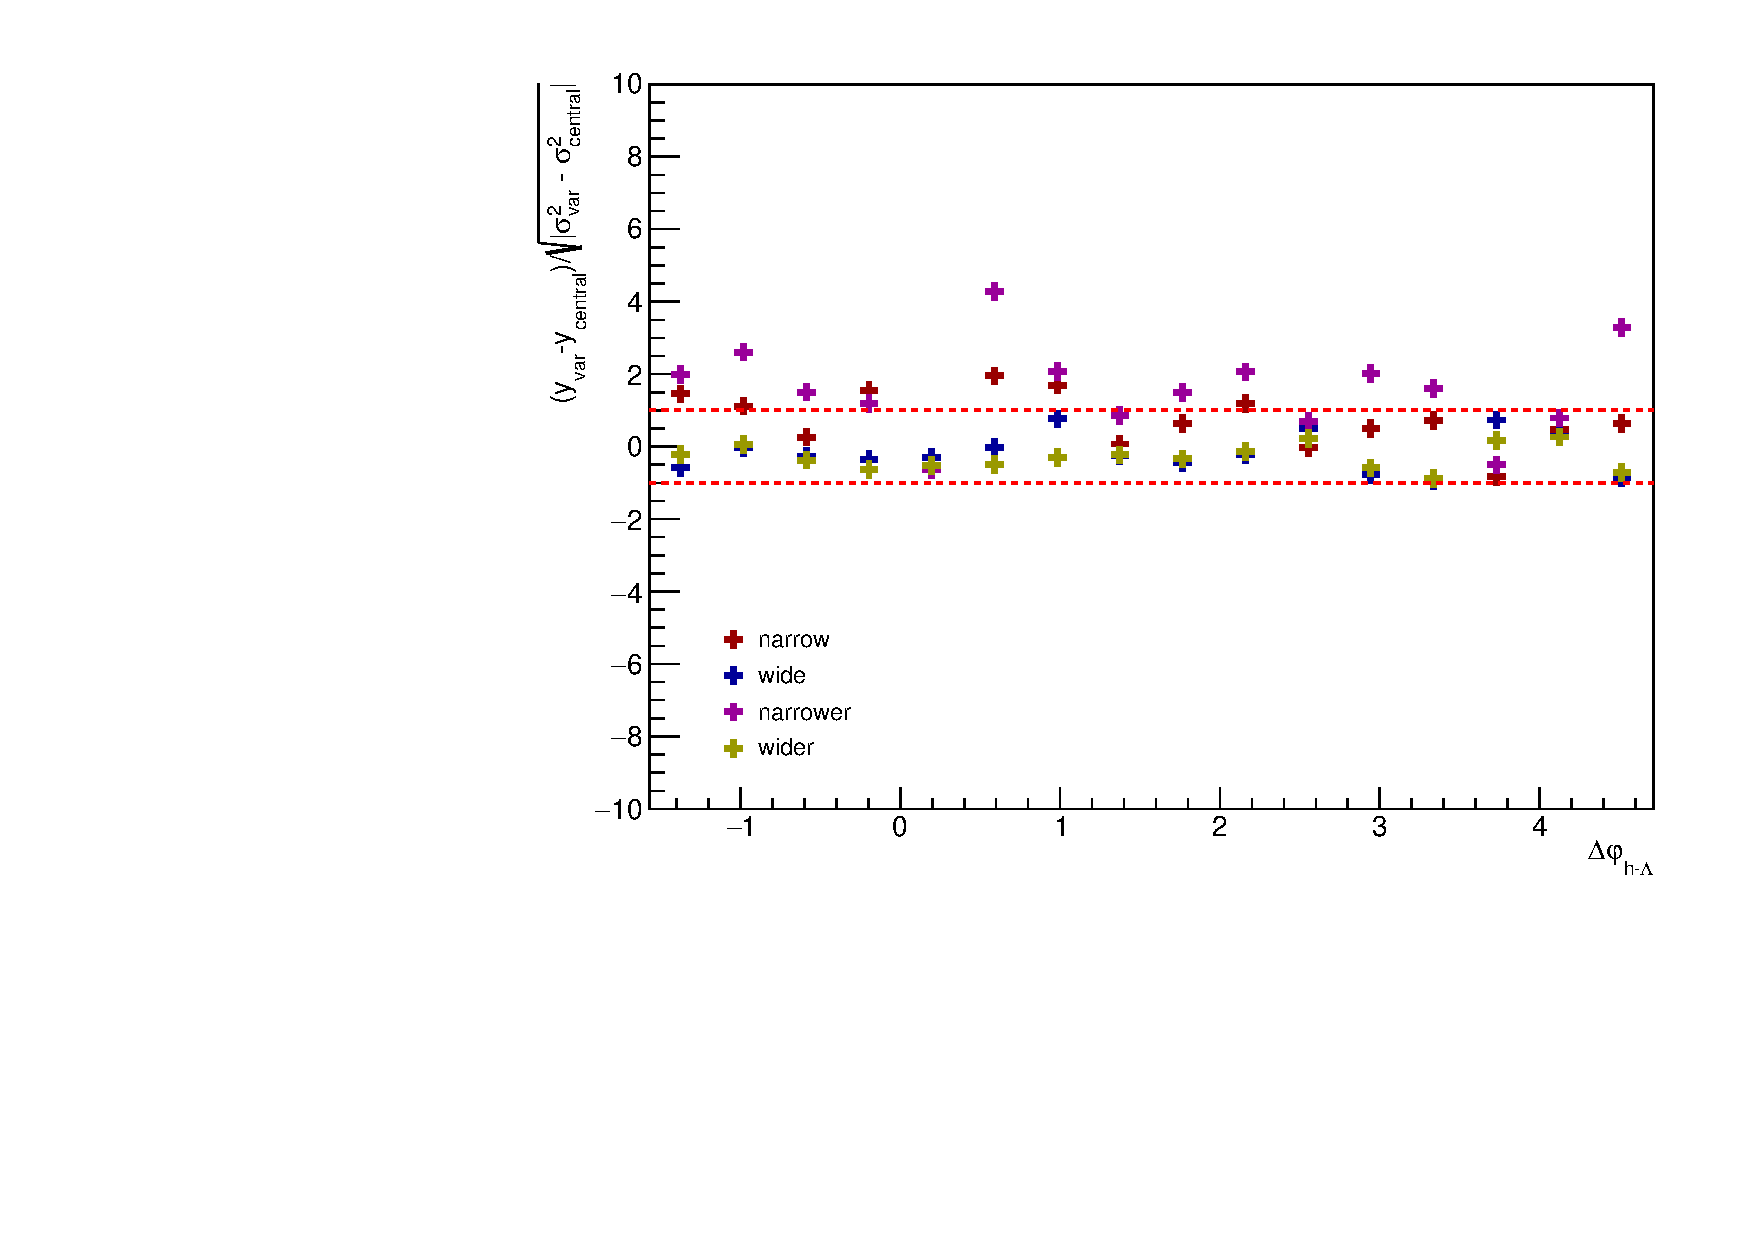
\includegraphics[width=0.32\textwidth]{figures/analysis/signal_barlow_0_20.pdf}
    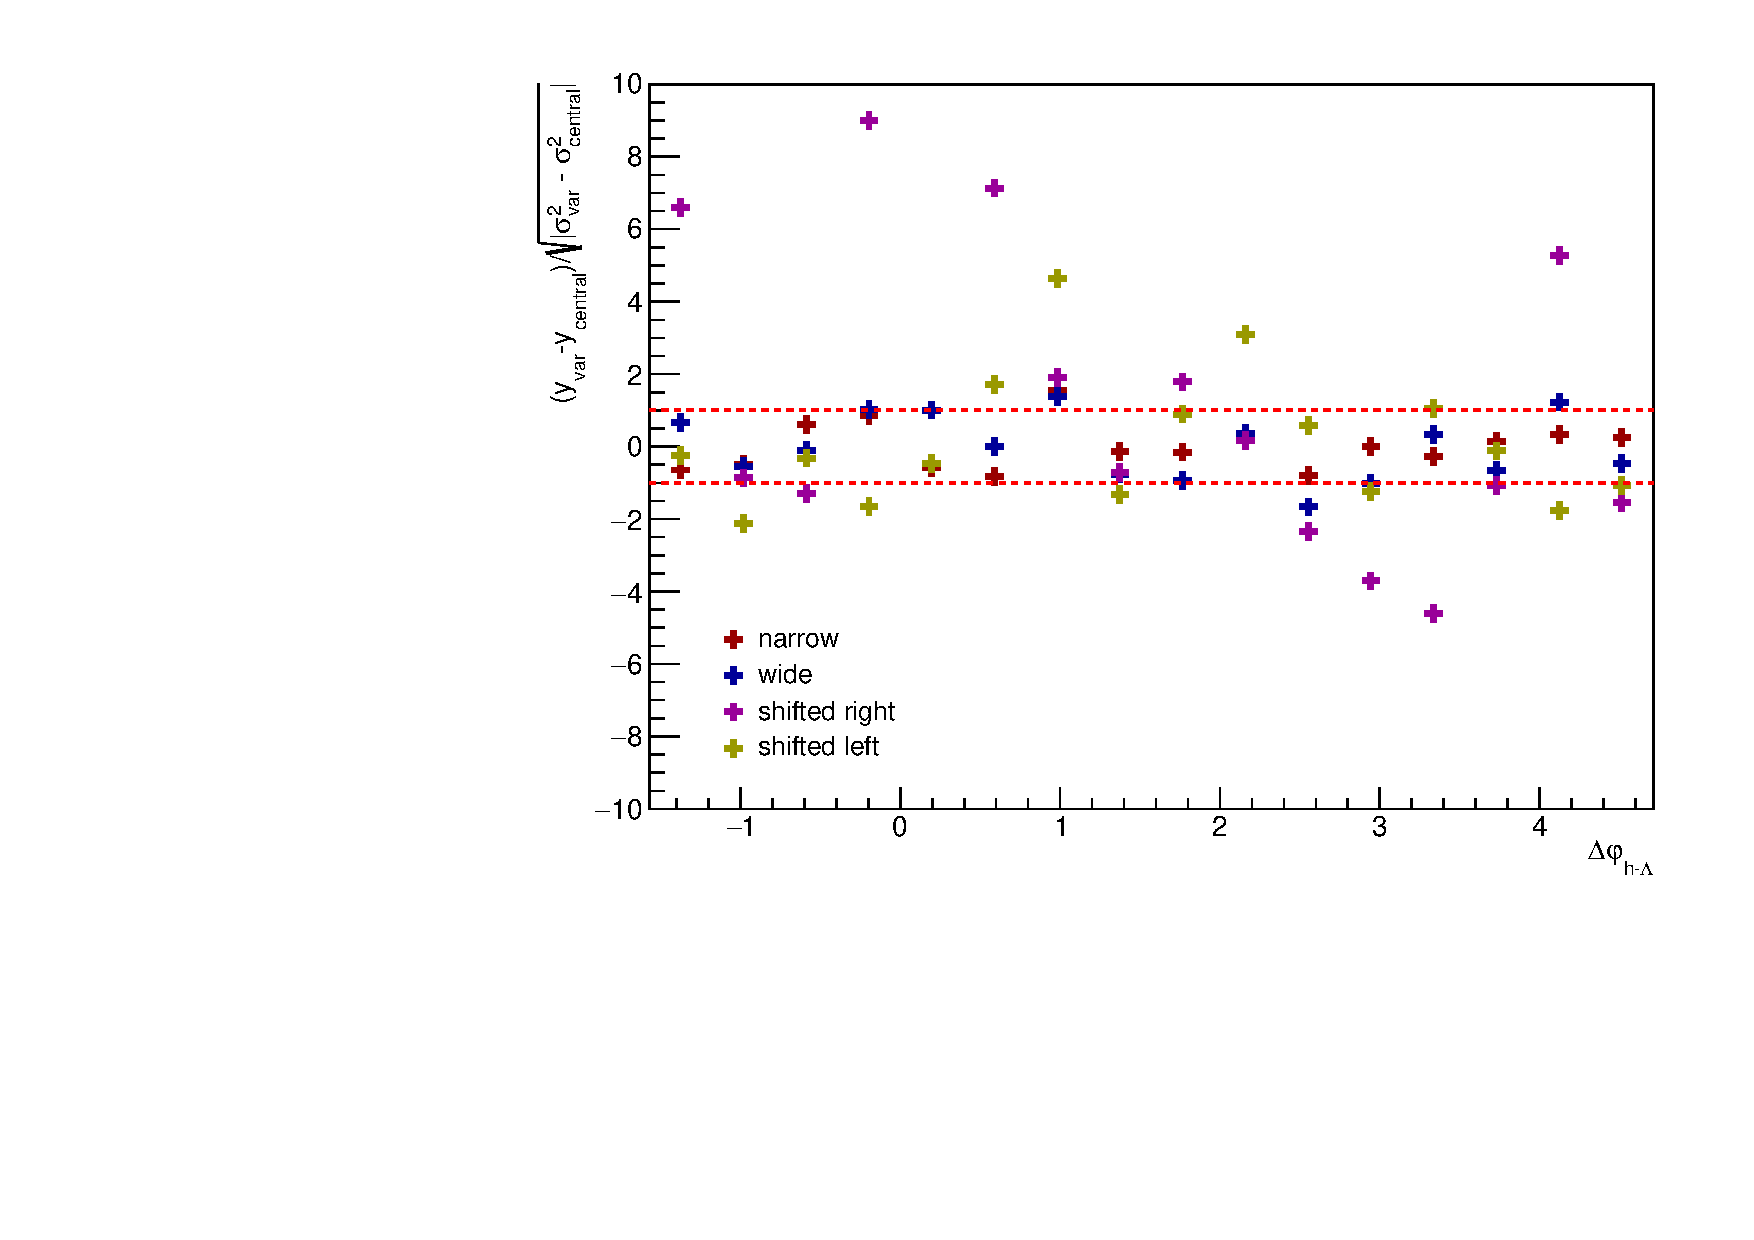
\includegraphics[width=0.32\textwidth]{figures/analysis/sideband_barlow_0_20.pdf}
    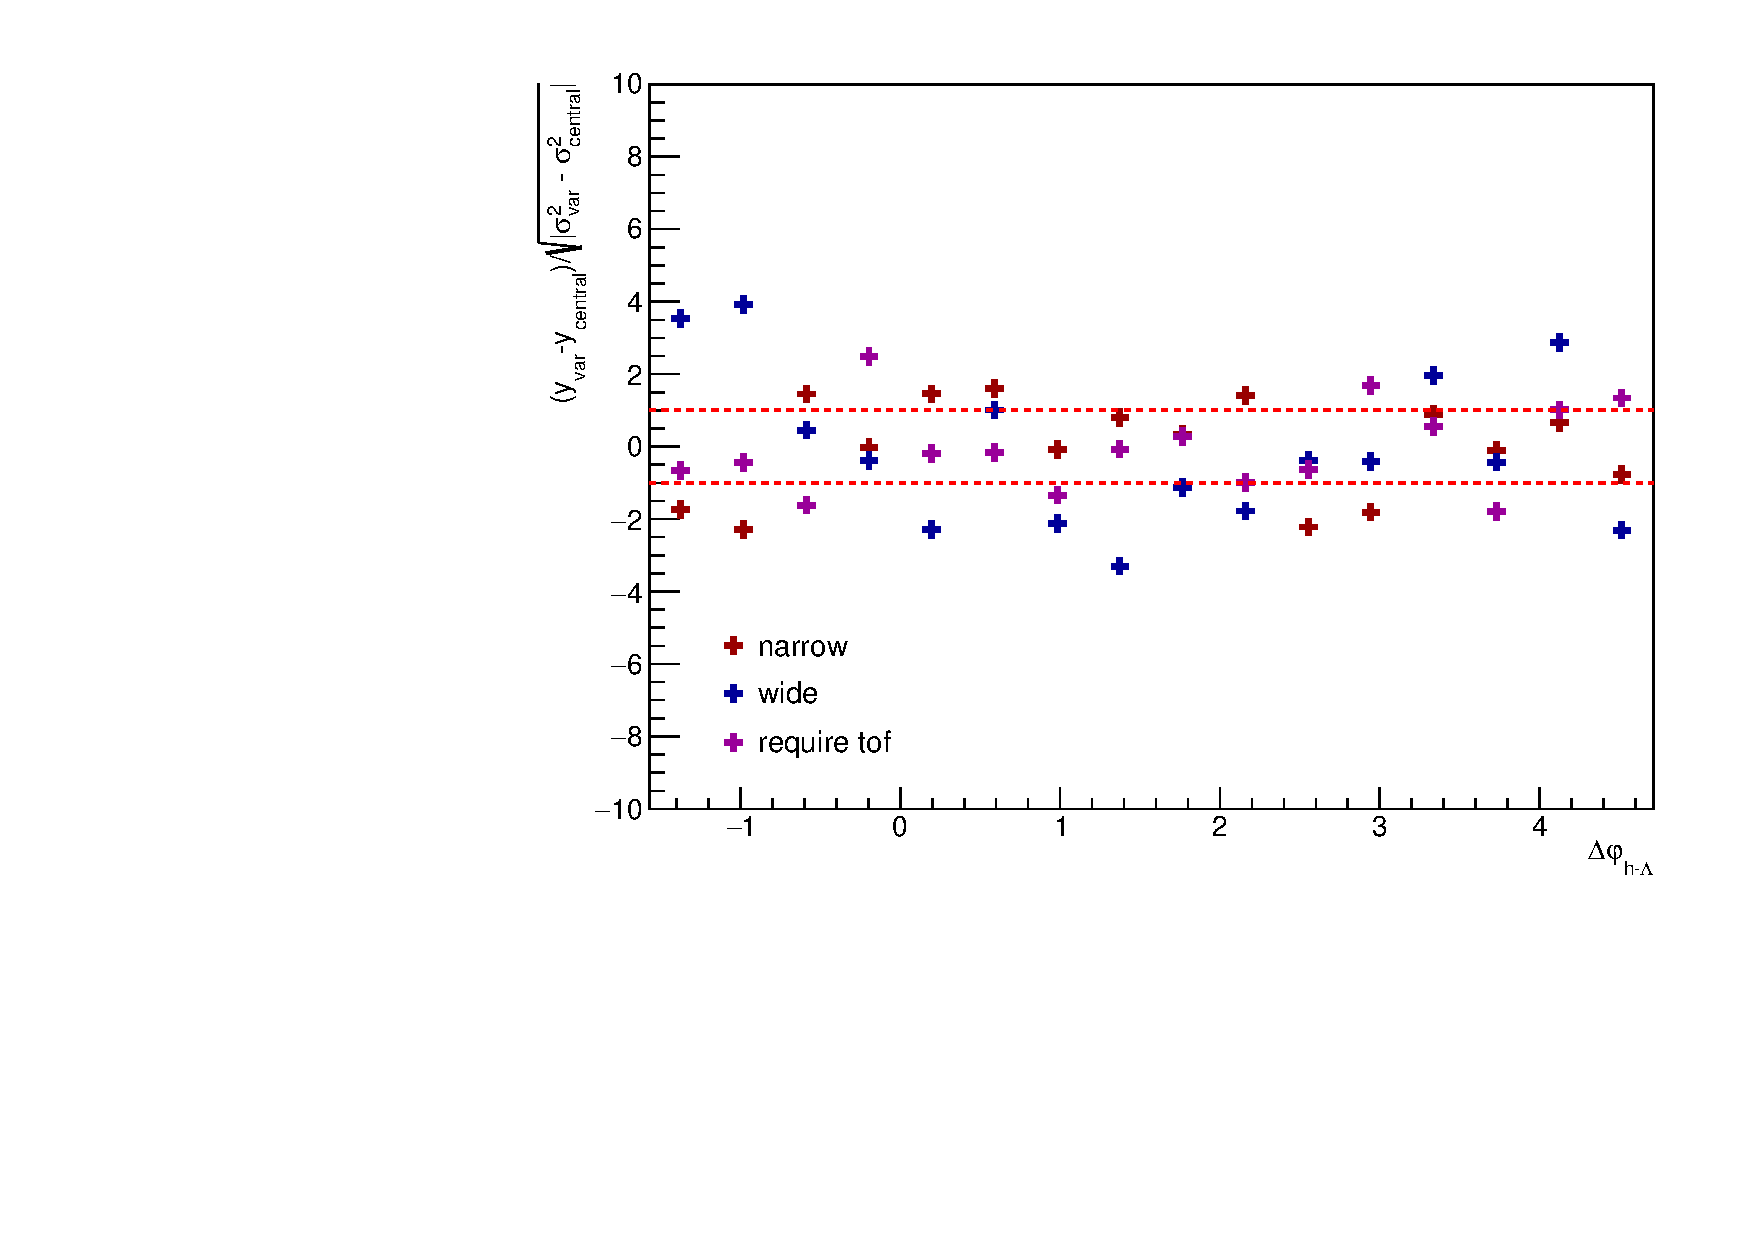
\includegraphics[width=0.32\textwidth]{figures/analysis/pid_barlow_0_20.pdf}
    \caption{Barlow check for the signal (left), sideband (middle), and PID (right) variations in the 0-20\% multiplicity bin. The red lines represent $N\sigma_{RB} = \pm 1$, and if the majority of the points fall within the red lines (across all $\Delta\varphi$, multiplicty and \pt bins), they are excluded from the systematic uncertainty calculation.}
    \label{fig:barlow_check_0_20}
\end{figure}

As a result of the check, the following variations are excluded from the final systematic uncertainty calculation:
%
\begin{itemize}
    \item Signal: wide, wider
    \item Sideband: wide, narrow
    \item PID: require TOF
\end{itemize}
%
These exclusions are not so surprising. As the nominal signal region is already fairly wide, making it wider does not significantly change the $\Delta\varphi$ distribution. Similarly, the initial sideband region falls fairly close to the signal region. So long as there are enough statistics in the corresponding sideband h-$\Lambda$ distribution, changing its width should not affect the $\Delta\varphi$ distribution in a meaningful way. It also appears that requiring a TOF hit introduces large statistical errors, which dominate the denominator in Equation~\ref{eq:barlow_check}.

\subsubsection{$\Delta\varphi$ distribution systematics, summarized}
\label{sec:dphi_systematics_summarized}

The final systematic errors (after the Barlow check) from the h-\lmb $\Delta\varphi$ distribution generation for each multiplicity bin and \pt bin are shown in Table \ref{tab:h_lambda_dphi_systematics_table}. The total systematic uncertainty is calculated by adding each systematic error in quadrature. This table is consolidated into plots showing the systematic errors for each multiplicity bin and \pt bin, which are presented in Figure \ref{fig:dphi_systematics_plots}. As the systematic uncertainties associated with the generation of the dihadron $\Delta\varphi$ distributions are only from the tracking efficiency presented in Table~\ref{tab:flat_systematics}, they are not plotted in this section.

\begin{table}[ht]
    \centering
    \caption{The final systematic uncertainties (in percentages) from the h-$\Lambda$ $\Delta\varphi$ distribution generation for each multiplicity and associated \pt bin.}
    \label{tab:h_lambda_dphi_systematics_table}
    \begin{tabular}{l c c c c c c}
        \hline
        Mult. and \pt bin & Sig. & Sideband & PID & Topo. sel.  & Mat. bud. & Total \\
        \hline
        \hline
        0-20\%, low \pt & 0.36 & 0.53 & 0.64 & 3.2 & 1.1 & 3.3 \\
        20-50\%, low \pt & 0.35 & 0.67 & 0.65 & 3.2  & 1.1 & 3.4 \\
        50-80\%, low \pt & 0.76 & 1.1 & 1.4 & 3.2  & 1.1 & 3.8 \\
        0-20\%, high \pt & 0.42 & 0.42 & 0.76 & 3.0 & 0.6 & 3.2 \\
        20-50\%, high \pt & 0.4 & 0.71 & 1.2 & 3.0  & 0.6 & 3.3 \\
        50-80\%, high \pt & 1.1 & 1.6 & 2.0 & 3.0  & 0.6 & 4.1 \\
        \hline
    \end{tabular}
\end{table}


\begin{figure}[ht]
    \centering
    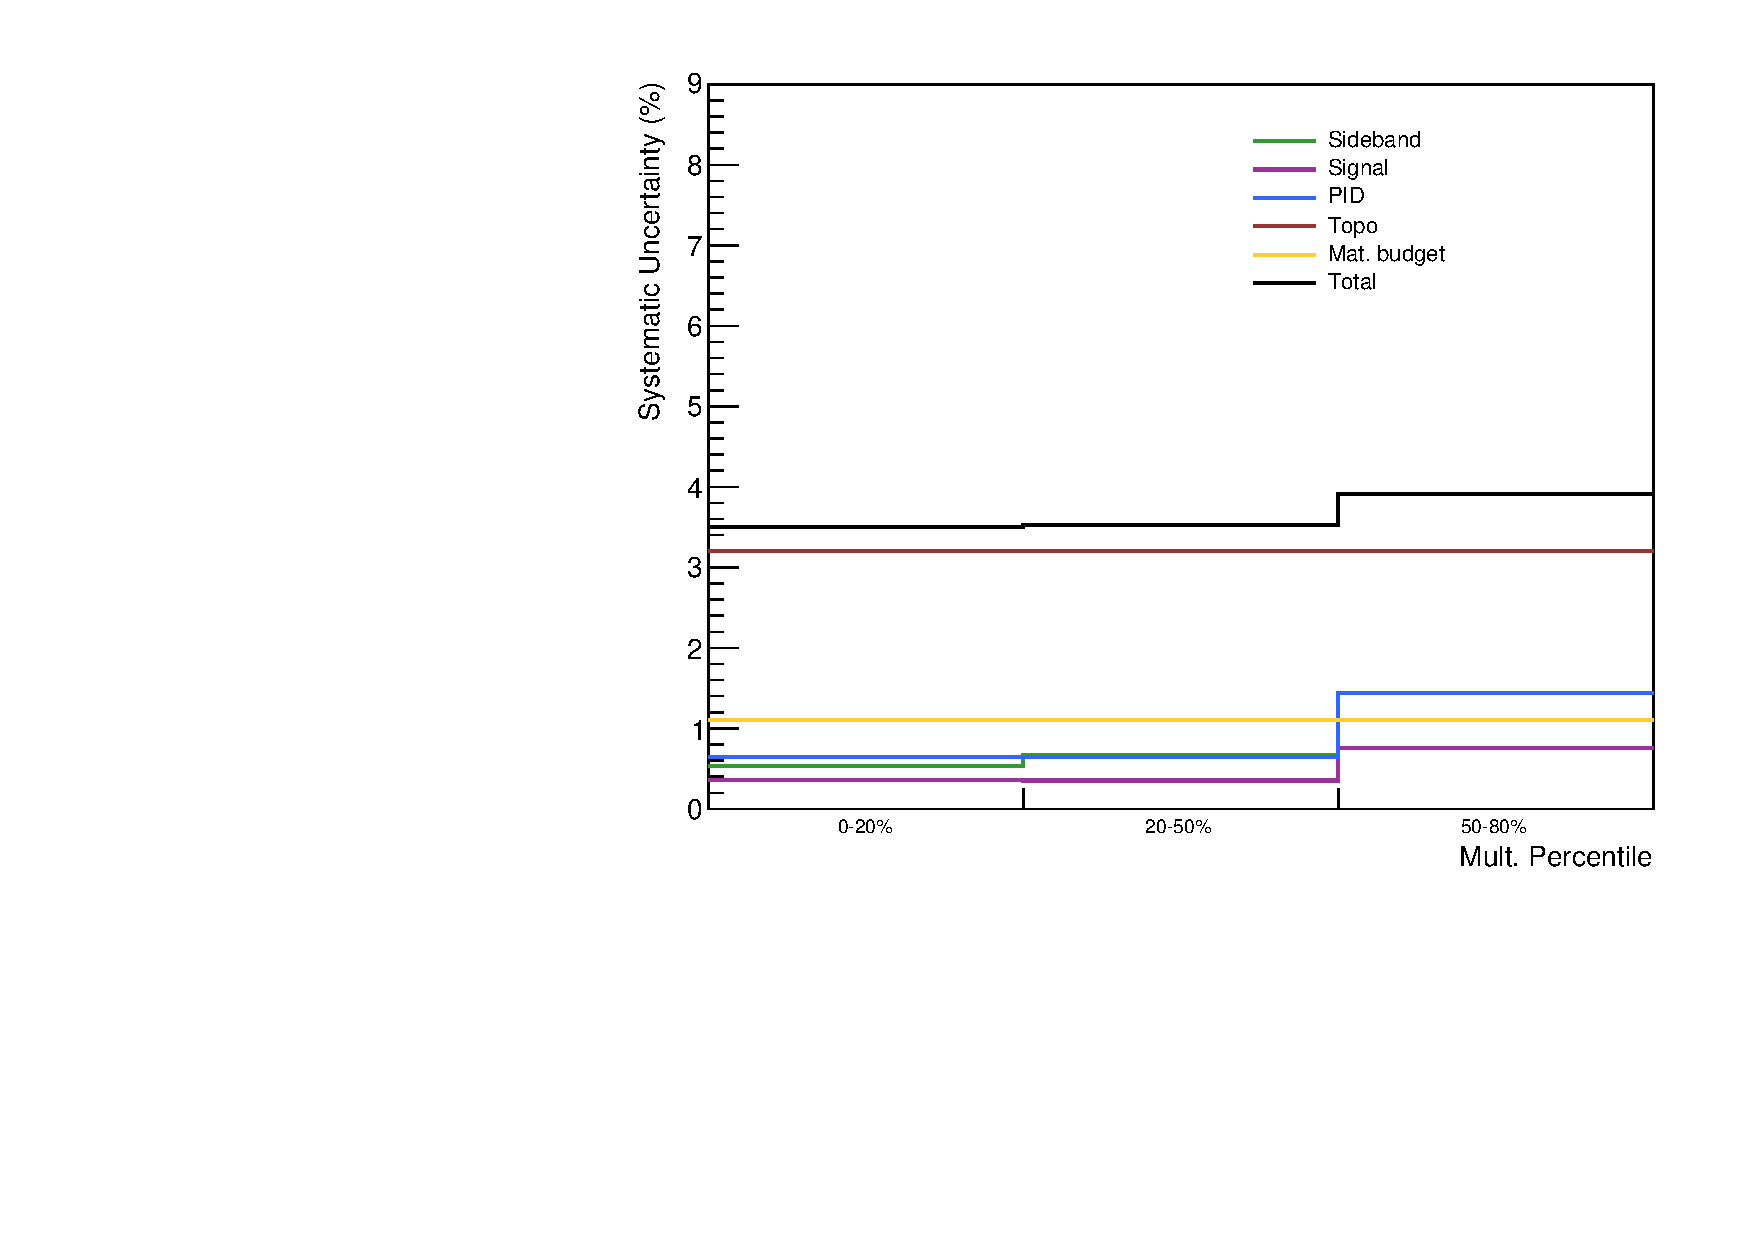
\includegraphics[width=0.48\textwidth]{figures/analysis/systematics_dphi_postbarlow_lowpt.pdf}
    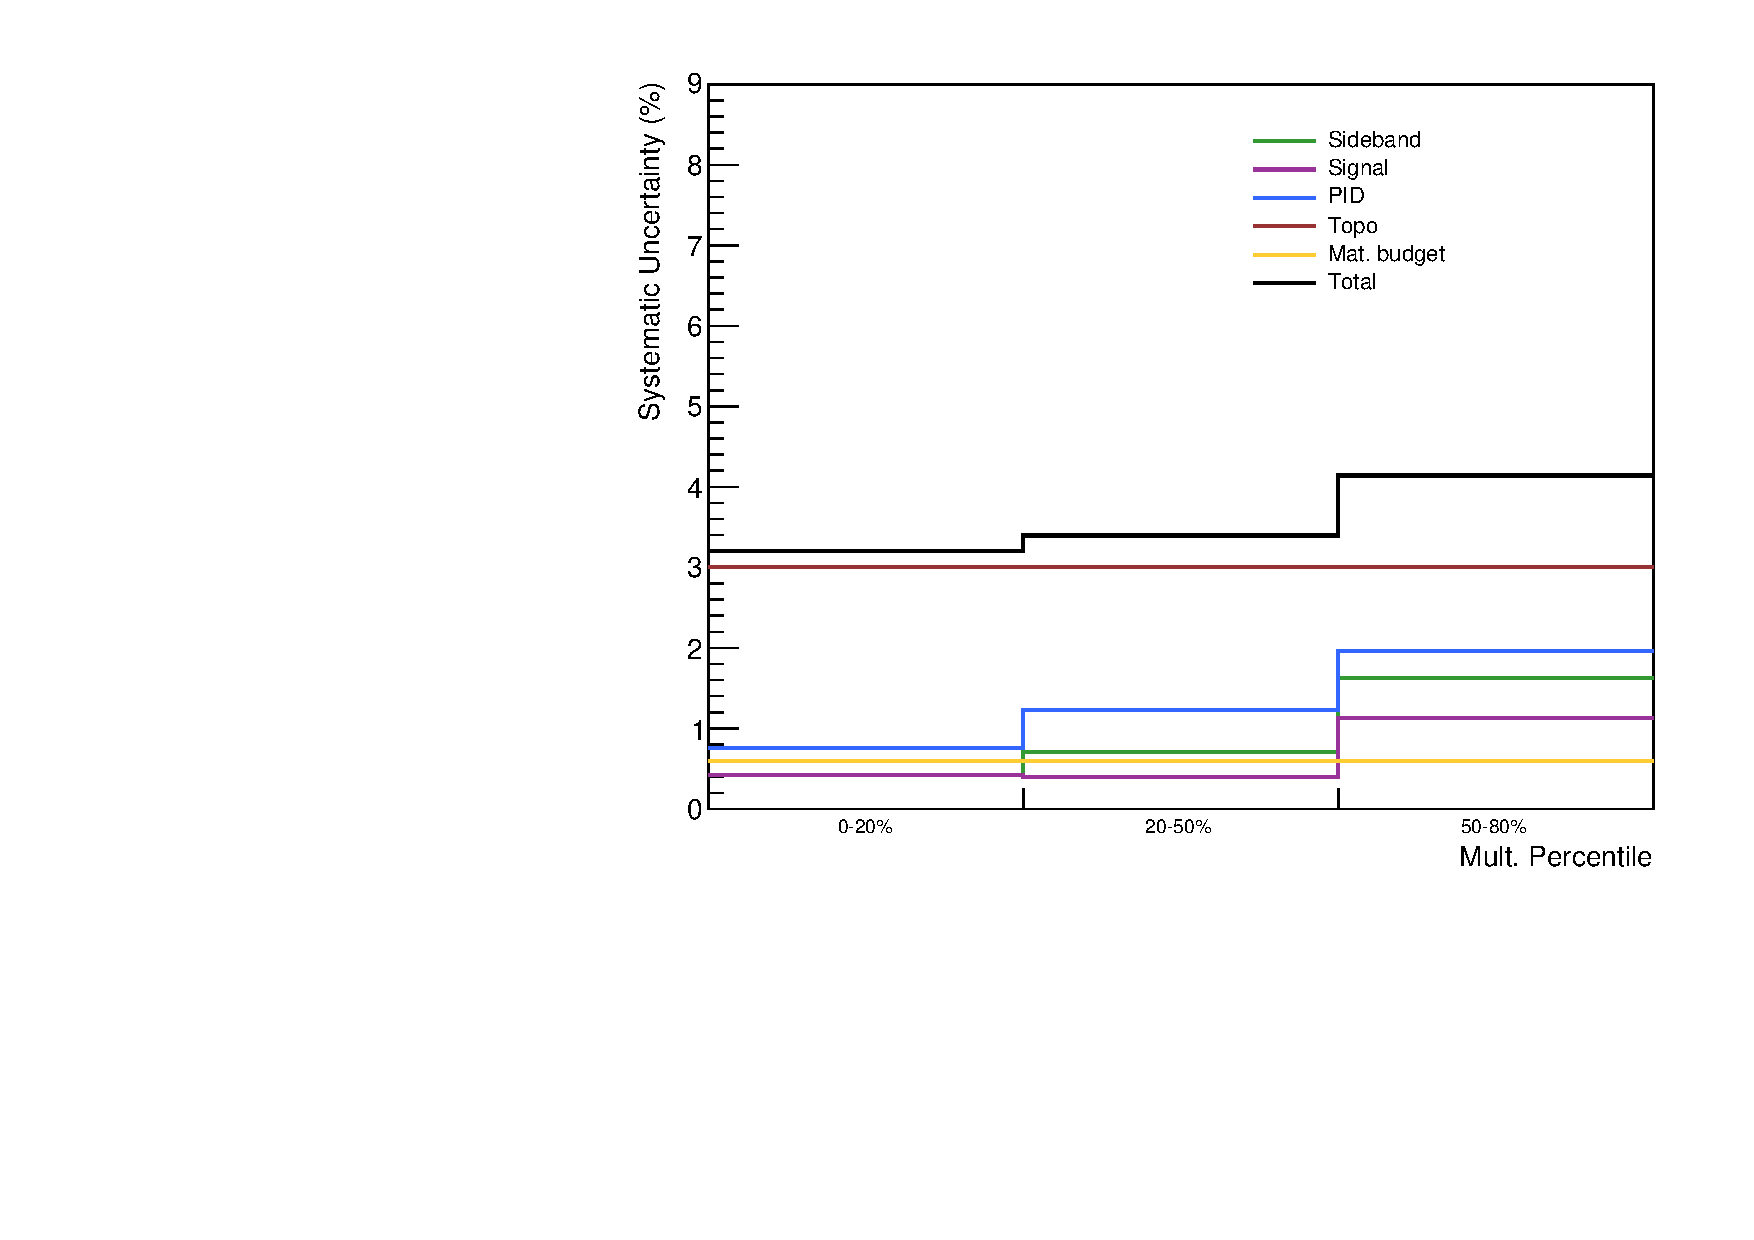
\includegraphics[width=0.48\textwidth]{figures/analysis/systematics_dphi_postbarlow_highpt.pdf}
    \caption{A visual depiction of the final systematic errors for the h-$\Lambda$ $\Delta\varphi$ distributions for each multiplicity bin in the low (left) and high (right) associated \pt bins. The total systematic error is shown in black.}
    \label{fig:dphi_systematics_plots}
\end{figure}

The total systematic error is observed to be mostly $p_{T}$-independent. However, there appears to be a slight correlation between the systematic uncertainty and multiplicity, with the 0-20\% bin exhibiting lower uncertainties than the 50-80\% bin across both \pt ranges. This can become problematic when investigating the multiplicity dependence of observables extracted from the $\Delta\varphi$ distributions, as the fraction of the systematic uncertainty which is directly correlated with multiplicity should not be considered when measuring multiplicity-dependent trends like slopes and percent changes. Because of this, the fraction of the systematic uncertainty which is uncorrelated with multiplicity is approximated using
%
\begin{equation}
    \label{eq:uncorrelated_fraction_1}
    \sigma_{\text{uncor}, i}^2 = \sum_{\text{vars}}(R_{\text{var}, i} - 1)^2,
\end{equation}
where 
\begin{equation}
    \label{eq:uncorrelated_fraction_2}
    R_{\text{var}, i} = (\frac{y_{\text{var}, i}}{y_{\text{nom}, i}})/ (\frac{y_{\text{var}}^{MB}}{y_{\text{nom}}^{MB}}),
\end{equation}
%
where ``i'' refers to the ith multiplicity bin, and ``MB'' refers to the min-bias (multiplicity-integrated) results. The deviations of $R_{\text{var}, i}$ from unity quantify how the deviations in multiplicity bin $i$ differ from those in the MB sample. $\sigma_{\text{uncor}, i}$ is computed for each $\Delta\varphi$ bin, then the RMS is taken across all $\Delta\varphi$ bins to obtain the final multiplicity-uncorrelated portion of the systematic errors. The results for each \pt bin are shown in Figure~\ref{fig:dphi_nch_dep_systematics_plots}. These systematic errors are only used when quantifying the multiplicity dependence of an observable extracted from the $\Delta\varphi$ distributions.

\begin{figure}[ht]
    \centering
    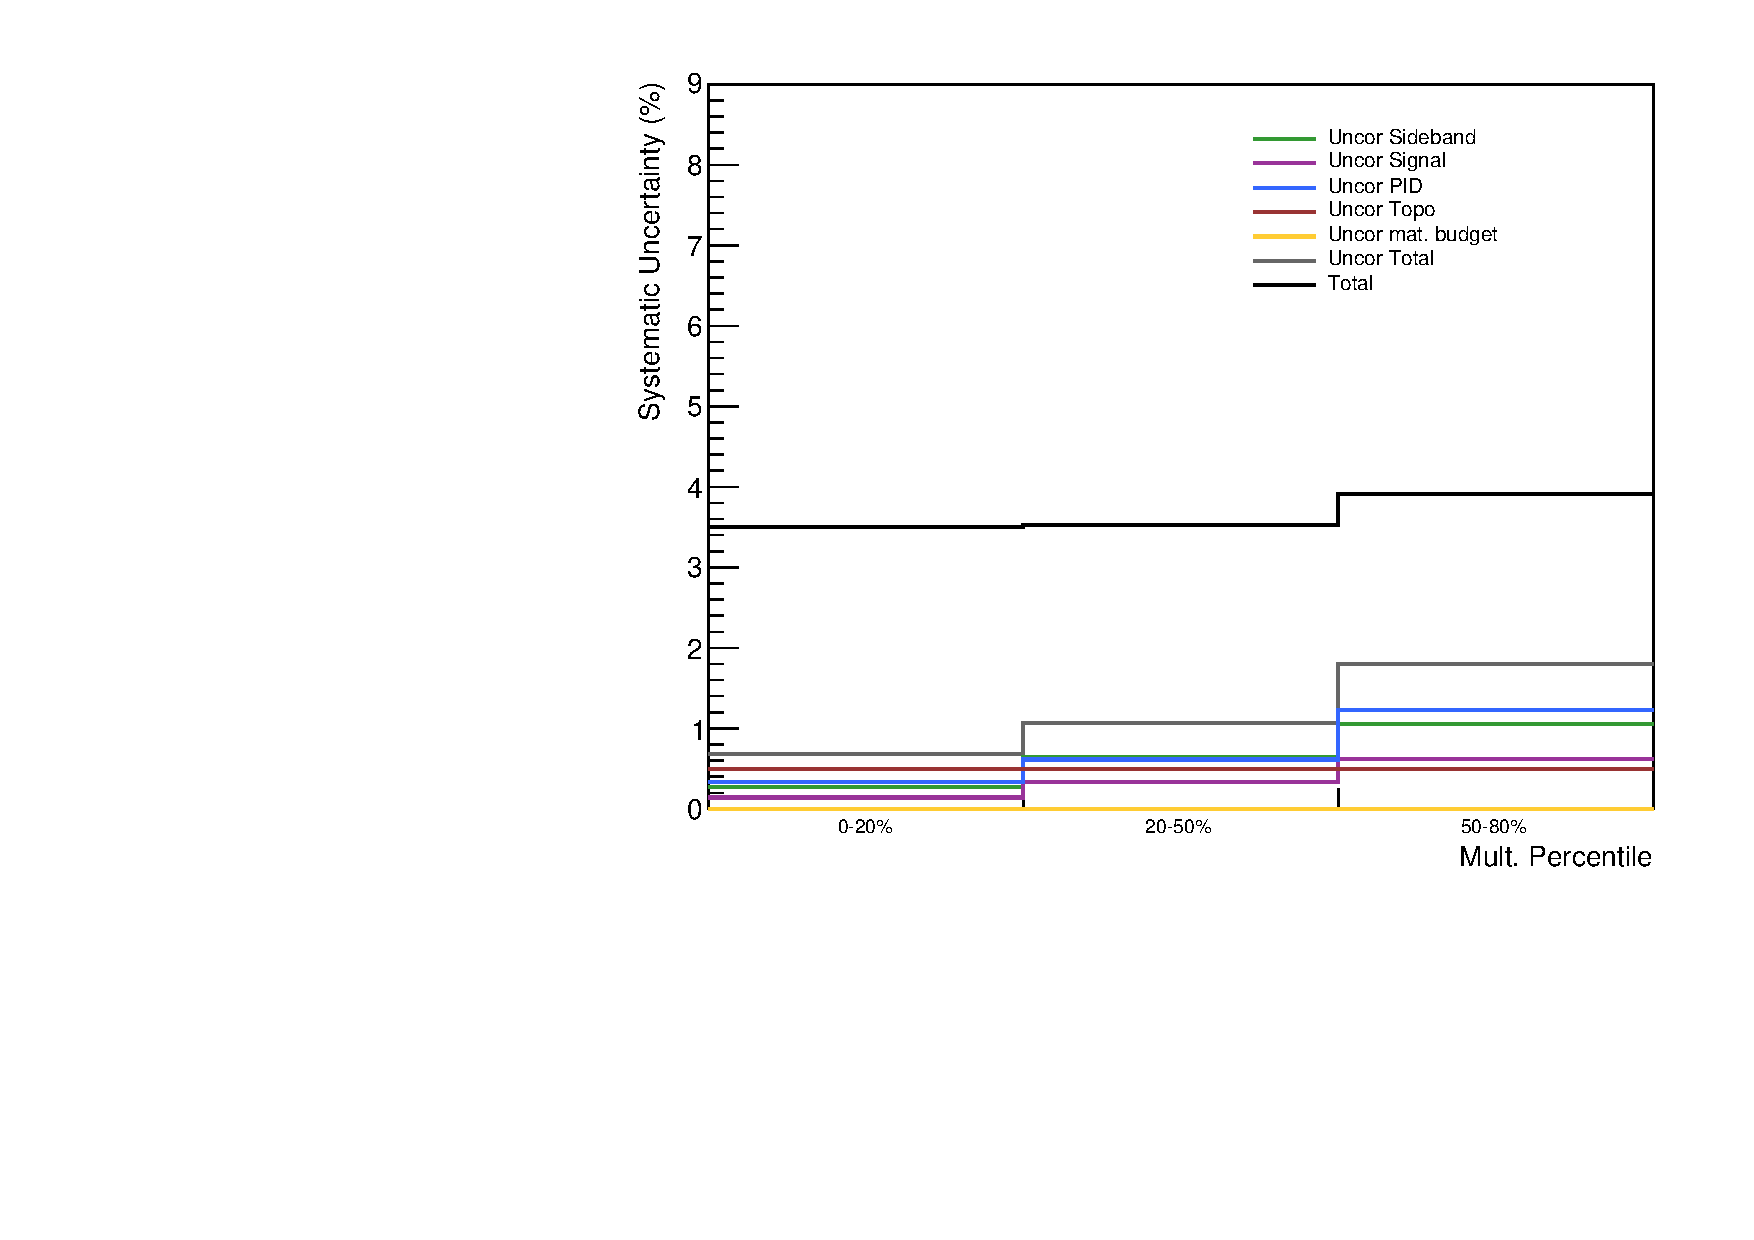
\includegraphics[width=0.48\textwidth]{figures/analysis/nch_dep_systematics_dphi_postbarlow_lowpt.pdf}
    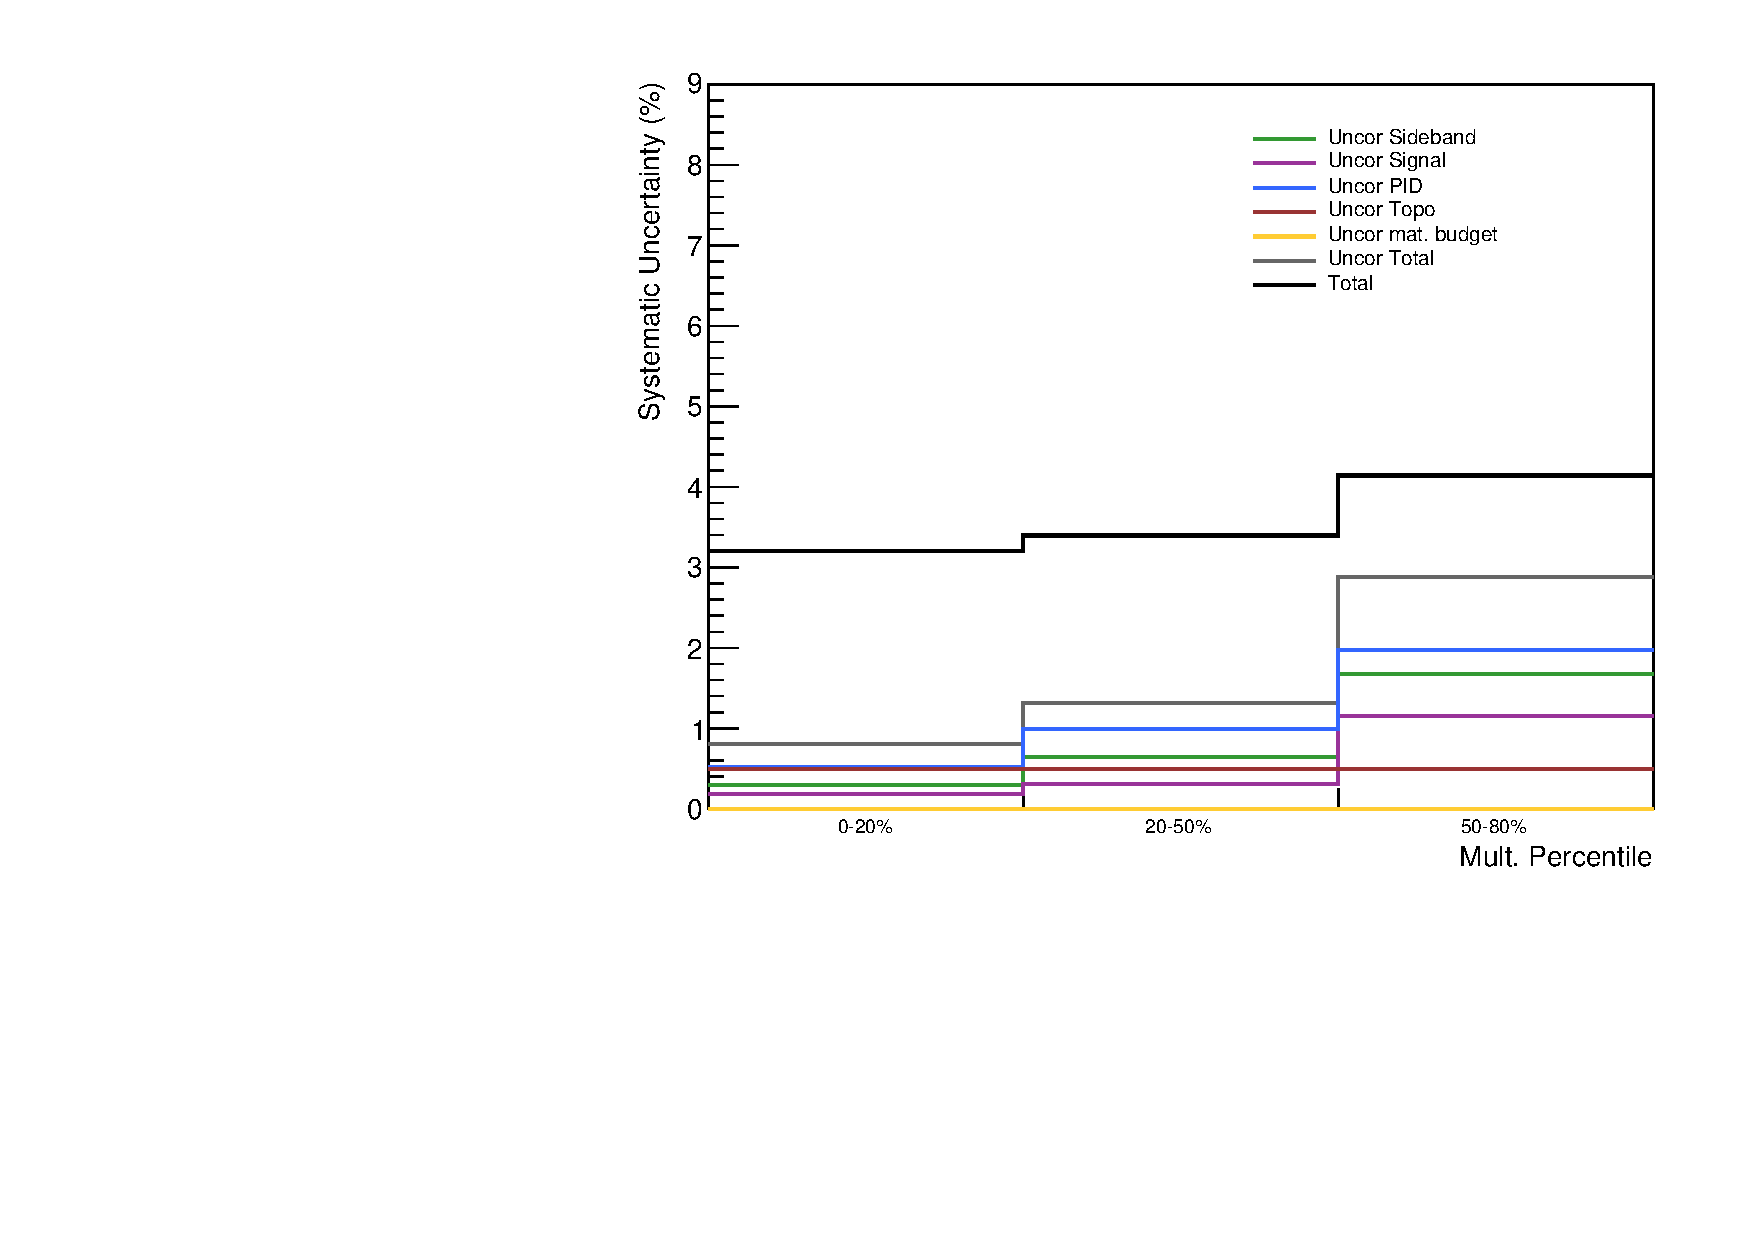
\includegraphics[width=0.48\textwidth]{figures/analysis/nch_dep_systematics_dphi_postbarlow_highpt.pdf}
    \caption{Visual depiction of the multiplicity-uncorrelated systematic errors for the h-$\Lambda$ $\Delta\varphi$ distributions for each multiplicity bin in the low (left) and hig (right) associated \pt bins, along with the total systematic error shown in black.}
    \label{fig:dphi_nch_dep_systematics_plots}
\end{figure}

% \clearpage

\subsection{Yield extraction}
\label{sec:systematics_yield_extraction}

One of the largest sources of systematic uncertainty of this analysis corresponds to the different techniques that can be used to extract the yields in the near-side jet, away-side jet, and underlying event from the $\Delta\varphi$ distributions. As mentioned in Section~\ref{sec:yield_extraction}, the equations for extracting these yields are
%
\begin{eqnarray}
    Y_{near} = \int_{-\pi/2}^{\pi/2} (\frac{dN}{d\Delta\varphi}- U(\Delta\varphi))d\Delta\varphi,  \  \ Y_{away} = & \int_{\pi/2}^{3\pi/2} (\frac{dN}{d\Delta\varphi}- U(\Delta\varphi))d\Delta\varphi 
    \label{eq:jet_yields_ref}
    \\ 
    Y_{UE} = \int_{-\pi/2}^{3\pi/2} U(\Delta\varphi)d\Delta\varphi,
    \label{eq:ue_yield_ref}
\end{eqnarray}
%
where $\frac{dN}{d\Delta\varphi}$ is the $\Delta\varphi$ distribution and $U(\Delta\varphi)$ is the underlying event fit. As the $\Delta\varphi$ distribution is present in these equations, all of the previous variations concerning the generation of this distribution must be considered. However, these equations also naturally introduce two new categories of systematic uncertainty: those associated with the underlying event fit, and those associated with the integration of the $\Delta\varphi$ distribution. Both of these categories will be discussed in detail in the following sections.


\subsubsection{Underlying event fit techniques}
\label{sec:ue_fit_systematics}

As the underlying event term $U(\Delta\varphi)$ is present in every yield extraction equation above, any changes in the underlying event fitting procedure will affect the final yield measurements. To maintain compatibility with previous analyses (specifically for the dihadron correlations), the nominal underlying event fit is a straight line to the average of the $\Delta\varphi$ distribution in the ranges $[-\frac{\pi}{2}, -\frac{\pi}{4}) \cup [\frac{\pi}{4}, \frac{5\pi}{8}) \cup [\frac{11\pi}{8}, \frac{3\pi}{2})$. These ranges were initially chosen as there is expected to be little-to-no contamination from the jet components in each range. However, to investigate the effect the UE fitting procedure may have on the final yields, the following alternative methods were considered:
%
\begin{enumerate}
    \item Straight line fit in a more restricted range, specifically $[-\frac{\pi}{2}, -\frac{3\pi}{8}) \cup [\frac{3\pi}{8}, \frac{5\pi}{8}) \cup [\frac{11\pi}{8}, \frac{3\pi}{2})$
    \item Straight line fit using the Zero Yield At Minimum (ZYAM) technique, where the underlying event line is set to the minimum of the $\Delta\varphi$ distribution
    \item Sinusoidal fit which includes a non-zero $v_{2}$ contribution
\end{enumerate}
%
The first two techniques are similar enough to the nominal technique that they will not be explicitly shown in this section. Restricting the range of the flat fit region results in deviations from the nominal procedure of around 2\%, whereas the ZYAM technique gives much larger deviations at about 15\%. Ultimately the ZYAM procedure is not included in the final systematics calculation due to a physical incompatibility, whereby the presence of $v_{2}$ in the higher multiplicity $\Delta\varphi$ distributions causes the ZYAM procedure to massively underestimate the underlying event contribution.

Including a non-zero $v_{2}$ contribution is a much more involved procedure and requires new machinery to be developed, so it will be described in detail in the next section.

\subsubsection{Including a non-zero $v_{2}$ contribution}
\label{sec:ue_fit_v2}

All of the ``straight line'' UE fitting techniques are based on the flatness assumption of the non-jet part of the correlation in \dphi. This means that the dijet axis direction does not affect the non-jet particle distribution's overall shape within an event. However, as mentioned in Section~\ref{sec:collective_flow}, previous \PbPb, \pPb, and even \pp collision studies have shown that the QGP's collective flow components ($v_{1}$, $v_{2}$, etc.) influence the phase-space distribution of particles within an event. Using Fourier decomposition, the $\Delta\varphi$ distributions on an event-by-event basis can be written as
%
\begin{equation}
    \label{eq:dphi_fourier_decomposition}
    \frac{dN}{d\Delta\varphi} = a_{0} + \sum_{n=1}^{\infty}2a_{n}cos(n\Delta\varphi),
\end{equation}
%
where $a_{n}$ are the Fourier coefficients. As mentioned in the introduction, these coefficients have been shown~\cite{FlowDphi} to be related to the collective flow coefficients $v_{n}$ via
%
\begin{equation}
    \label{eq:fourier_vn_relation}
    v_{n} = \frac{a_{n}}{a_{0}}.
\end{equation}
%
This means that even without reconstructing the reaction plane within a specified event, the effects of collective flow are present in the $\Delta\varphi$ distributions. This manifests in the correlation distributions as an underlying event which is not flat with respect to $\Delta\varphi$, but rather sinusoidal. While this is in direct conflict to the initial assumption of a flat underlying event, this nominal choice was made to maintain compatibility with previous measurements of dihadron yields using correlation techniques, which also assume a flat UE in \dphi.

As the $v_{2}$ or ``elliptic flow'' coefficient is the most dominant of the collective flow coefficients measured in \pPb collisions~\cite{Justin111} in the \pt ranges for this analysis, it is the only one considered. Furthermore, the $v_{2}$ coefficients are exceedingly difficult to determine, with fully published papers solely dedicated to measuring the $v_{2}$ for different particle species and collision systems. Luckily, these coefficients have been measured by ALICE in \pPb collisions for both charged hadrons and \lmb baryons across a wide range of \pt~\cite{ALICEv2_1, ALICEv2_2}. As the \pt binning in this analysis is much wider, the weighted average 
%
\begin{equation}
    \label{eq:v2_weighted_average}
    v_{2}^{avg} = \frac{\int_{p_{T, min}}^{p_{T, max}}v_{2}(p_{T})\frac{dN}{dp_{T}}dp_{T}}{\int_{p_{T, min}}^{p_{T, max}}\frac{dN}{dp_{T}}dp_{T}},
\end{equation}
%
is used, where $p_{T, min}$ and $p_{T, max}$ are the minimum and maximum values of \pt in the bins from this analysis (namely $1.5 - 2.5$ and $2.5 - 4.0$ \GeVc). The $v_{2}(\pt)$ values for charged hadrons and \lmb baryons are taken from ~\cite{ALICEv2_1}, and $dN/dp_{T}$ is taken from the published \pt spectra for charged hadrons and \lmb baryons from ~\cite{ALICEpPbEnhancement}, plots of which can be seen in Figures~\ref{fig:v2_plot} ($v_{2}$) and \ref{fig:pt_spectra_plot} (\pt spectra). The values of $v_{2}^{avg}$ for each \pt bin are shown in Table~\ref{tab:v2_values}. Note that the trigger $v_{2}$ remains the same, as the trigger \pt range is fixed for this analysis. The $\Lambda$ $v_{2}$ is markedly higher than the charged hadron $v_{2}$, which ultimately manifests itself as a larger deviation from the nominal UE fit when compared to the dihadron case.
%
\begin{table}[t]
    \centering
    \caption{$v_{2}$ values used in this analysis for each associated \pt bin. The values were calculated as the weighted average of published \pt-differential $v_{2}$ measurements with the published \pt spectra, taken across the entire associated \pt range.}
    \label{tab:v2_values}
    \begin{tabular}{ l c c c c }
    \hline
    $p_{T}^{\text{assoc.}}$ & $v_{2}^{\text{trig.}}$ & $v_{2}^{\text{assoc. h}}$ & $v_{2}^{\text{assoc.} \Lambda}$ \\
    \hline
    1.5 - 2.5 & 0.092 & 0.100 & 0.075 \\
    2.5 - 4.0 & 0.092 & 0.119 & 0.137 \\
    \hline
    \end{tabular}
\end{table}
%
Unfortunately there are few multiplicity-dependent measurements of the $v_{2}$ coefficients for identified particle species. Because of this, the $v_{2}$ values from Table~\ref{tab:v2_values} are used only in the 0-20\% multiplicity bin, with the $v_{2}$ values for the 20-50\% and 50-80\% multiplicity bins taken as 0.85 and 0.50 times the 0-20\% value, respectively.

\begin{figure}[ht]
    \centering
    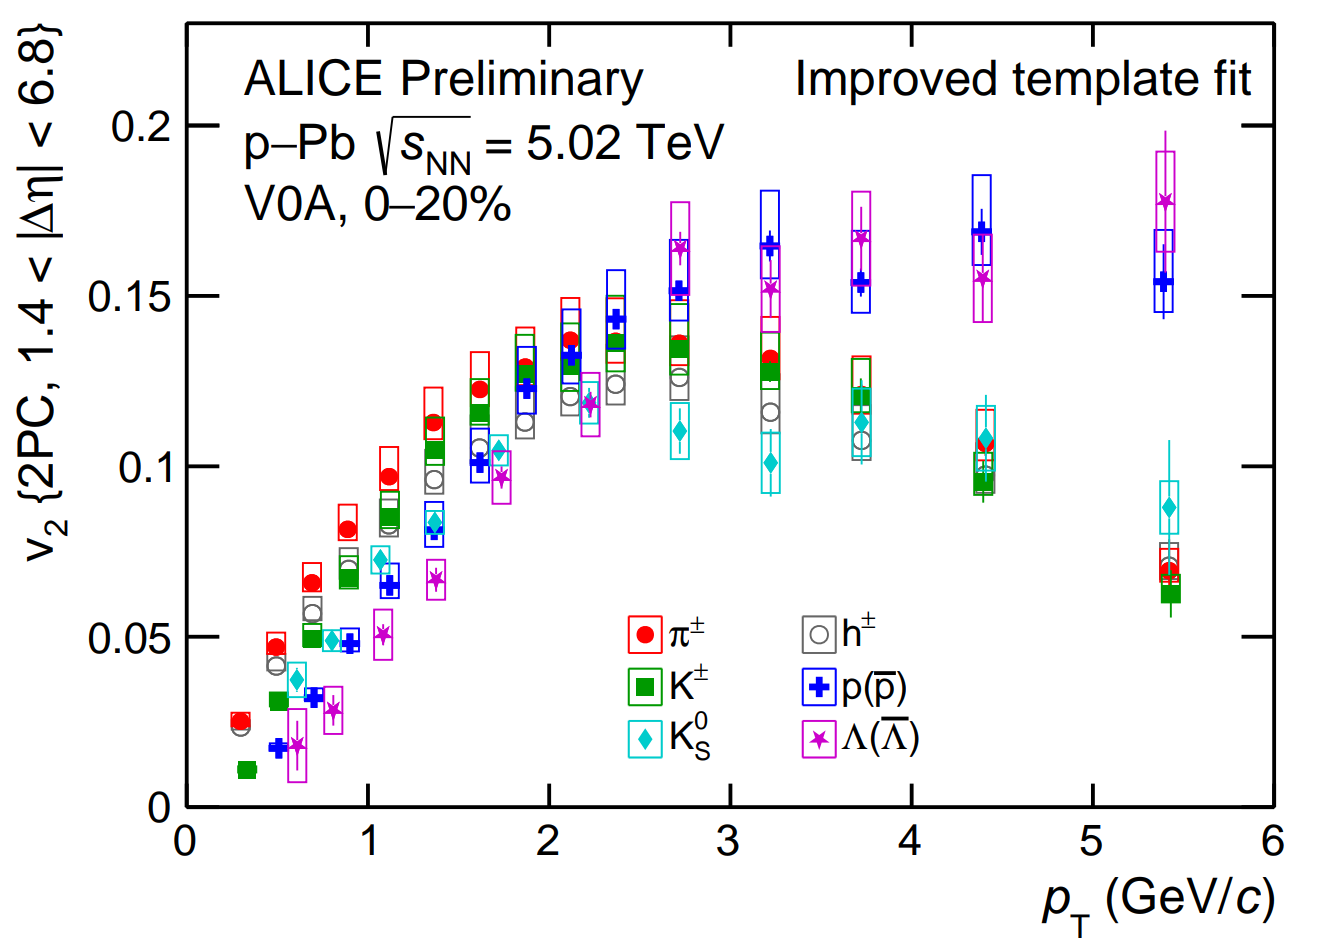
\includegraphics[width=0.8\textwidth]{figures/analysis/v2_diagram.png}
    \caption{The $v_{2}$ values for identified hadrons as a function of \pt, taken from~\cite{ALICEv2_1}.}
    \label{fig:v2_plot}
\end{figure}

\begin{figure}[ht]
    \centering
    \begin{minipage}{0.48\textwidth}
        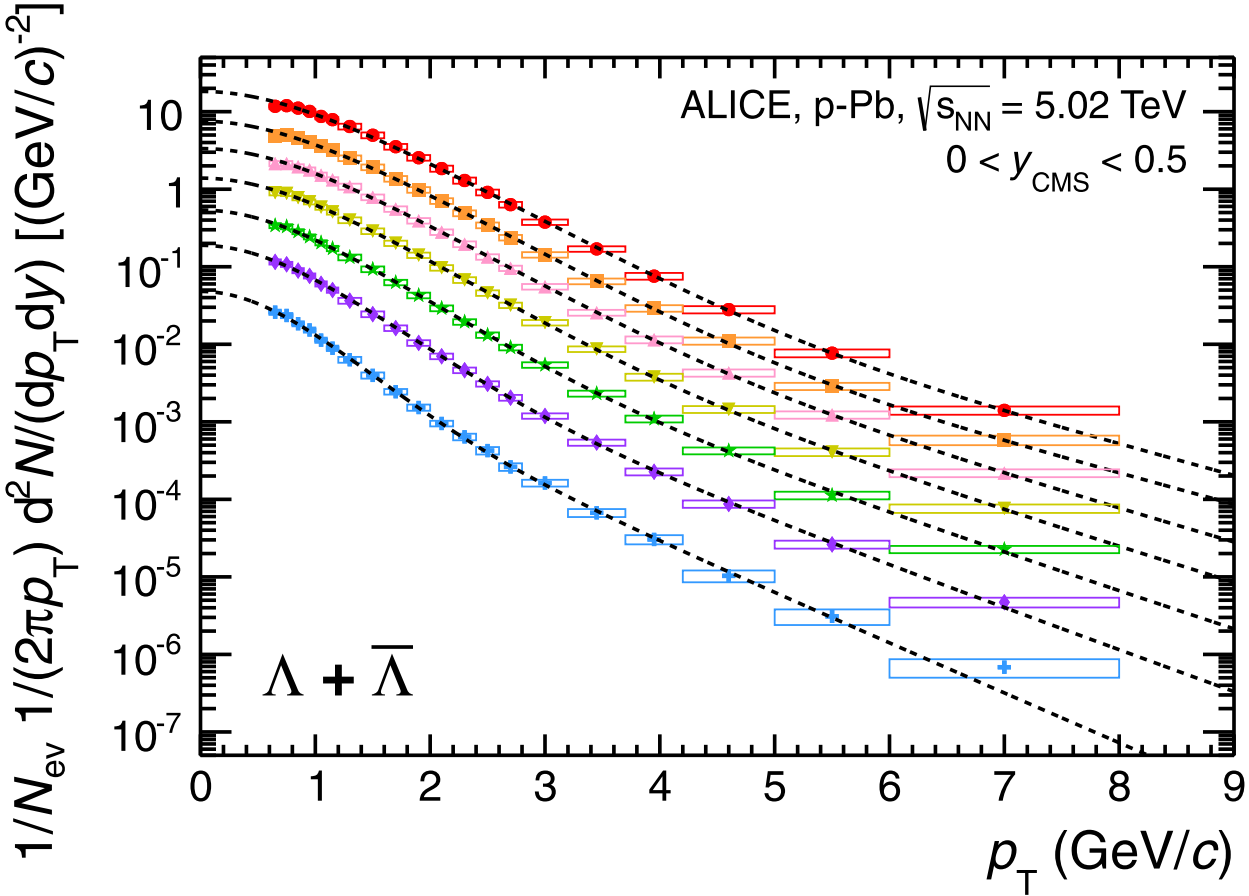
\includegraphics[width=\textwidth]{figures/analysis/lambda_pt_spectra.png}
        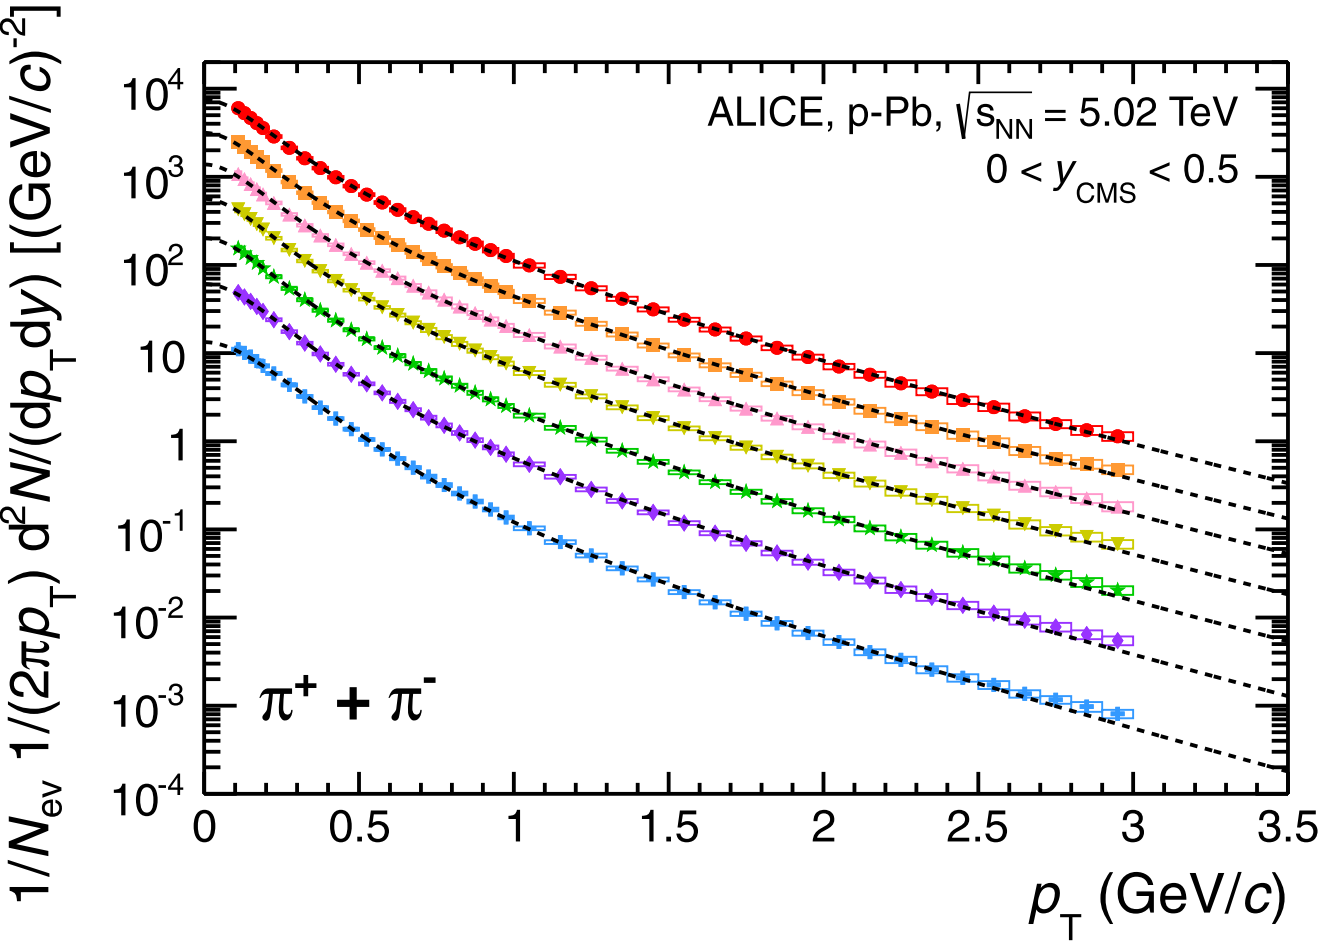
\includegraphics[width=\textwidth]{figures/analysis/pion_pt_spectra.png}
    \end{minipage}
    \hspace{1.2cm}
    \begin{minipage}{0.40\textwidth}
        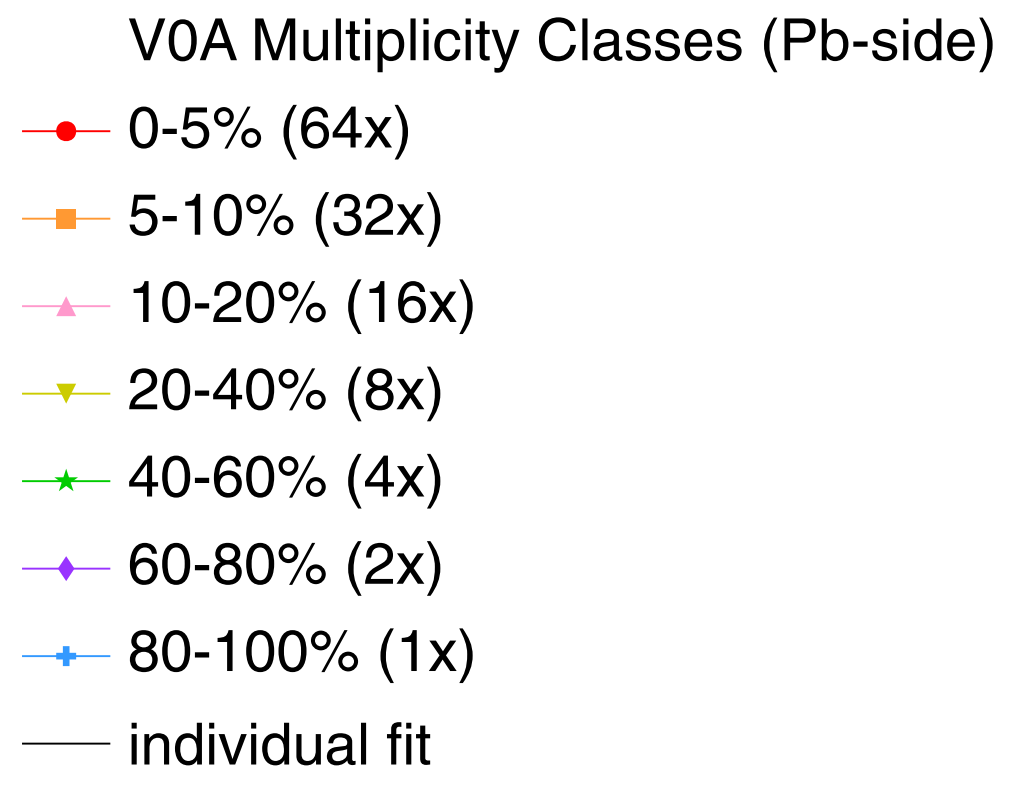
\includegraphics[width=0.8\textwidth]{figures/analysis/pt_spectra_legend.png}
    \end{minipage}
    \caption{The published~\cite{ALICEMatBud} \pt spectra for \lmb baryons (top) and charged hadrons ($\approx$ pions) (bottom), used to compute the weighted average of the $v_{2}$ coefficients across the wide momentum bins used in this analysis.}
    \label{fig:pt_spectra_plot}
\end{figure}

Using these $v_{2}$ values, the underlying event is estimated by fitting the function 
%
\begin{equation}
    \label{eq:ue_v2}
    U_{v_{2}}(\Delta\varphi) = A\times(1 + 2v_{2}^{\text{trig.}}v_{2}^{\text{assoc.}}cos(2\Delta\varphi))
\end{equation}
%
in the ranges $-\pi/2 < \Delta\varphi < -1$ and $1 < \Delta\varphi < +\pi/2$, where little jet contribution is expected. The underlying event \textbf{pedestal} $A$ is allowed to vary during the fit, but the $v_{2}$ values are fixed. Examples of h-\lmb and h-h $\Delta\varphi$ distributions with the UE fit using this procedure are shown in Figure~\ref{fig:v2_fit_examples}.

\begin{figure}[ht]
    \centering
    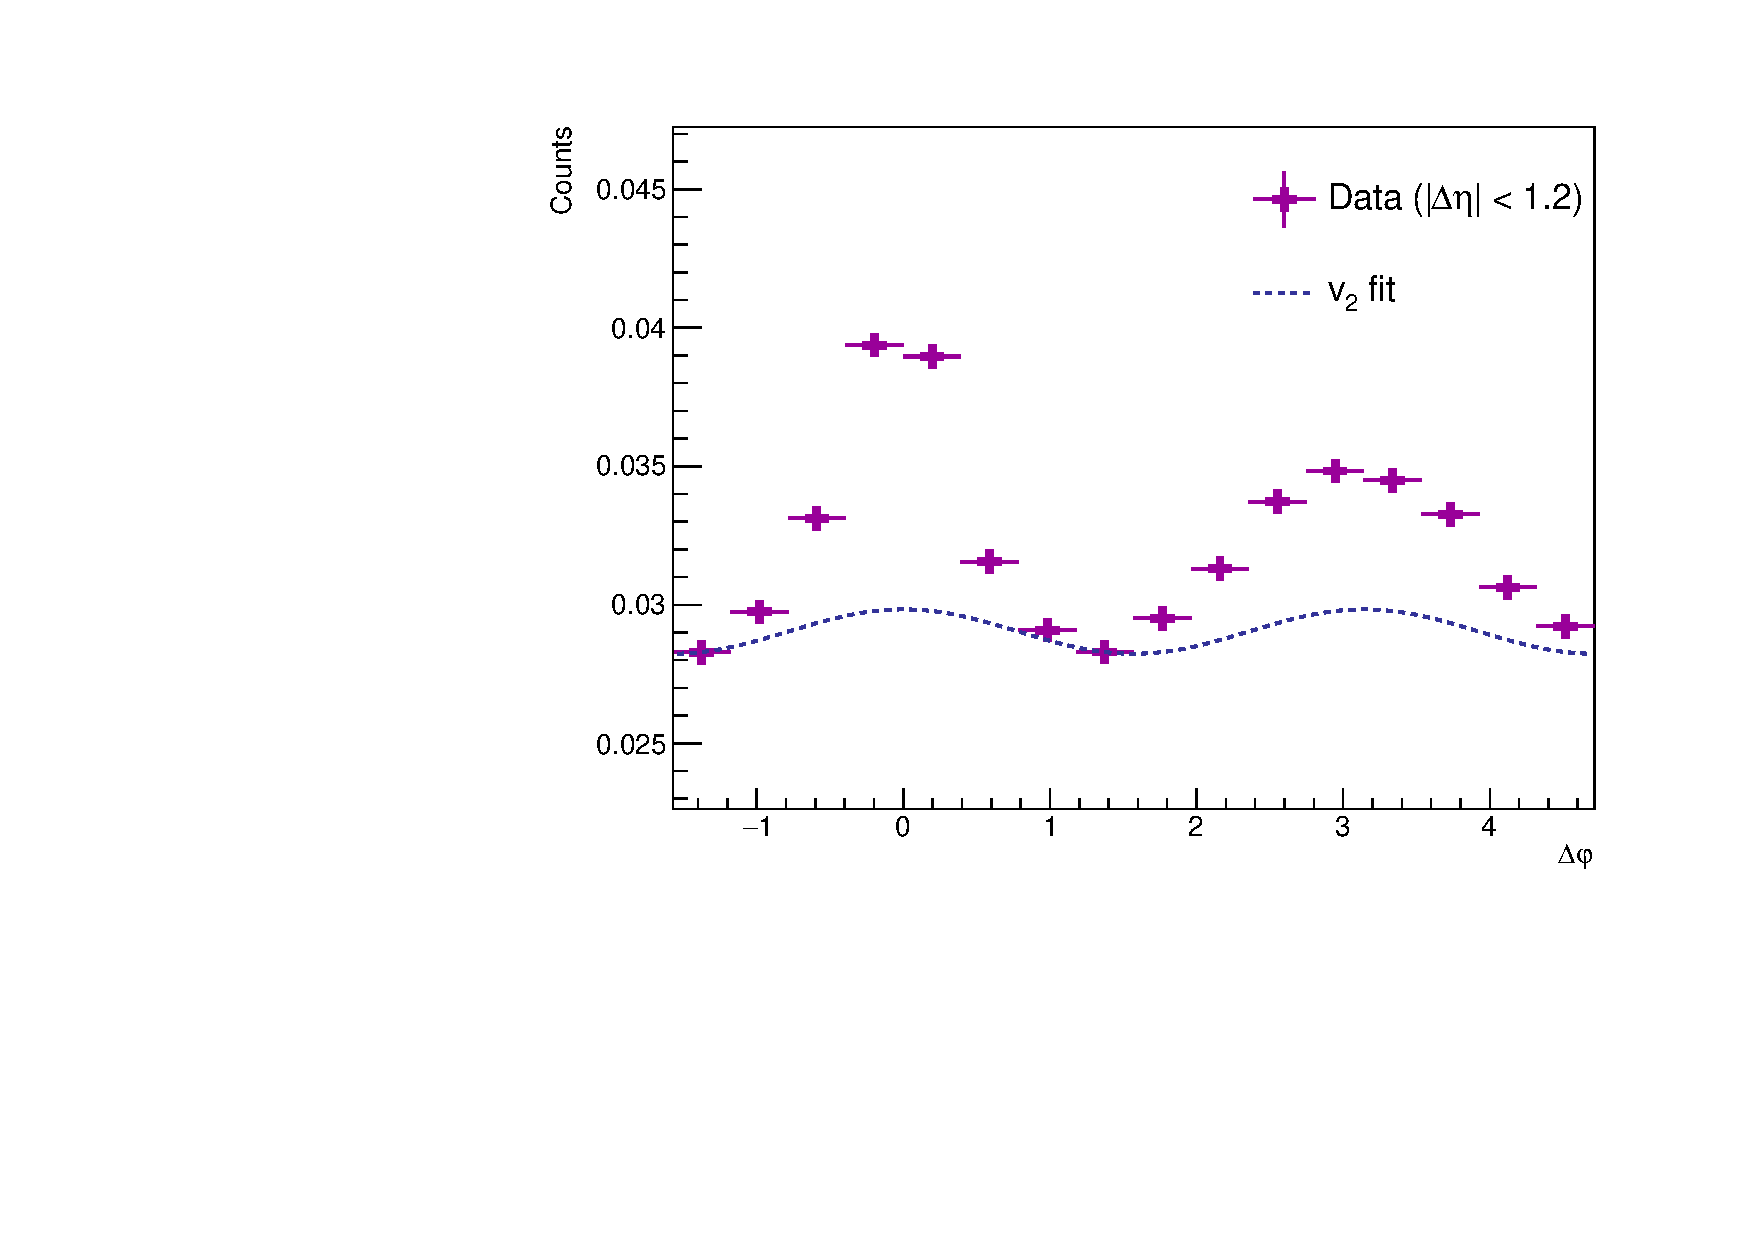
\includegraphics[width=0.49\textwidth]{figures/analysis/v2fit_h_lambda_cent_0_20_trigger_4_8_assoc_25_4.pdf}
    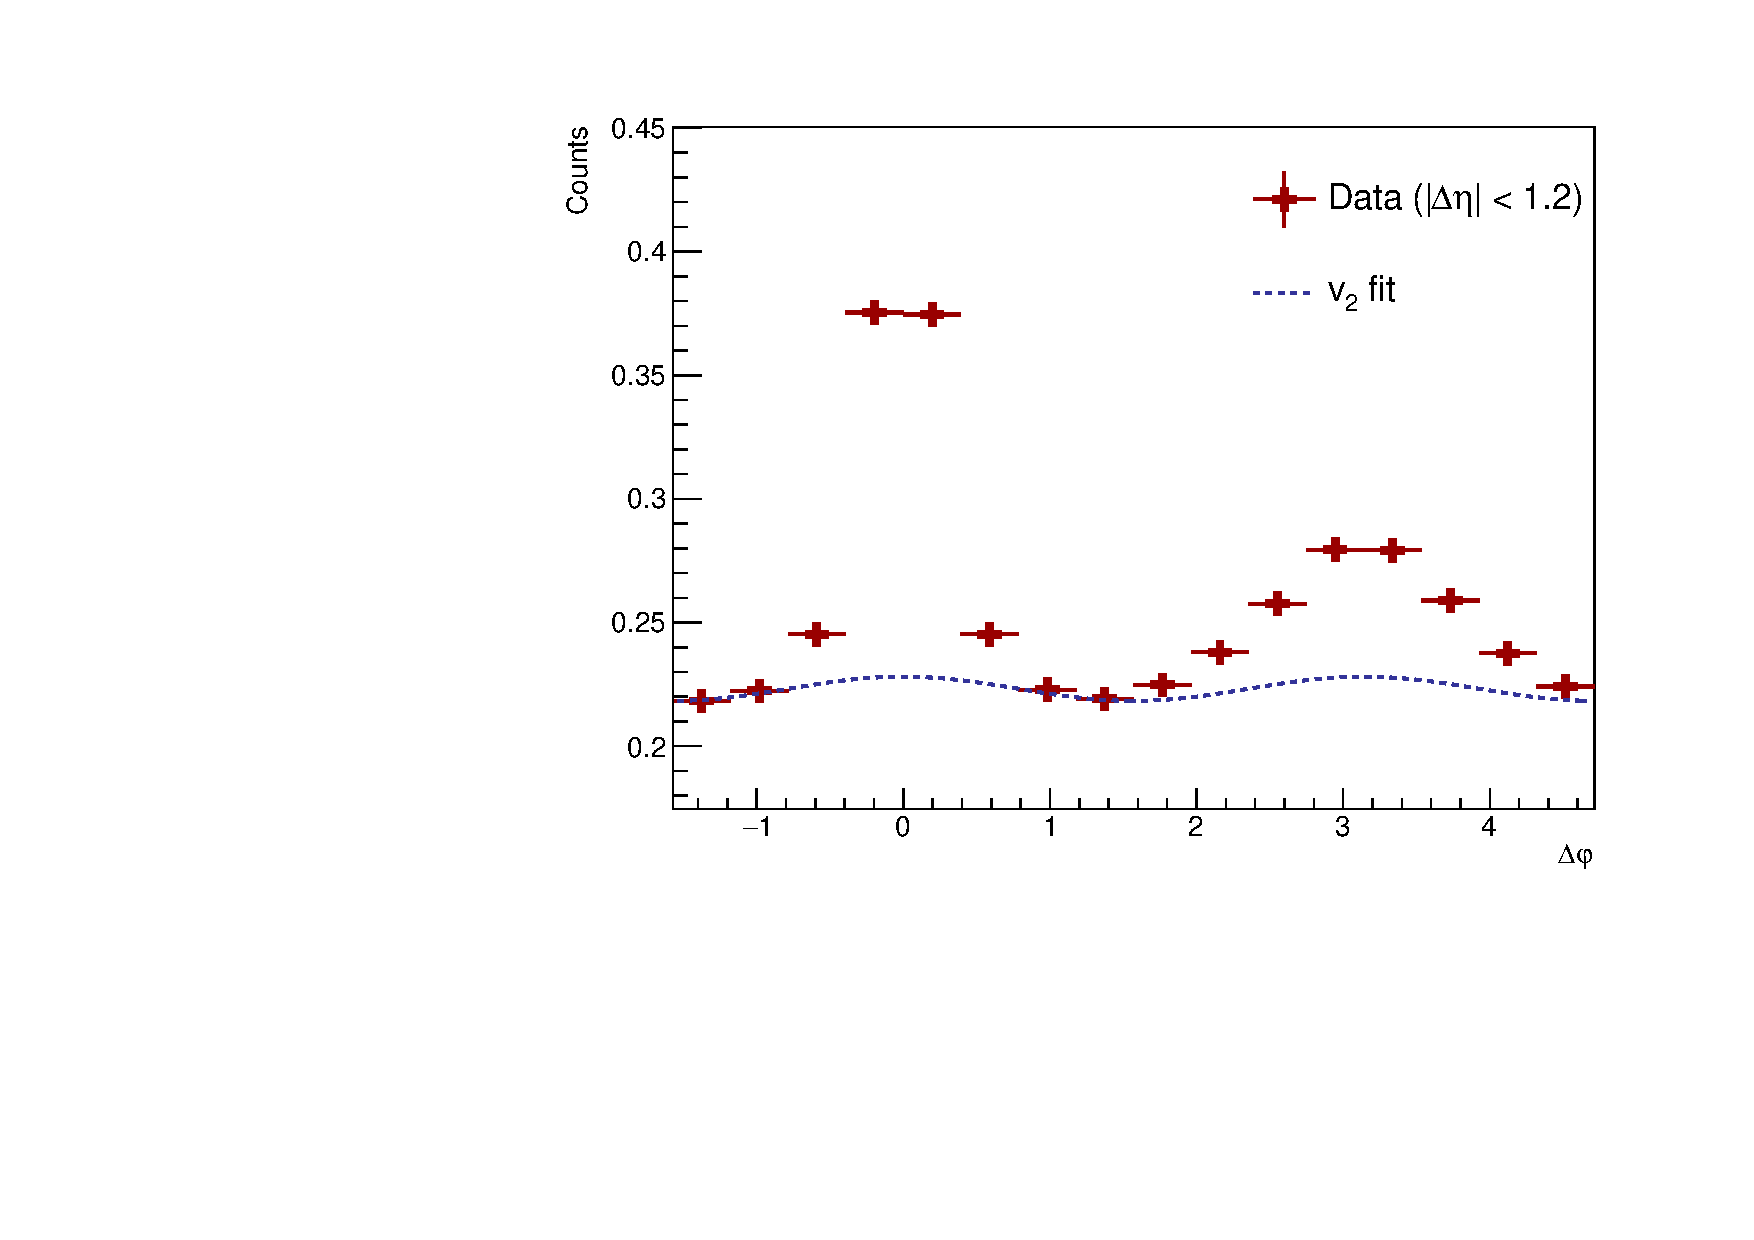
\includegraphics[width=0.49\textwidth]{figures/analysis/v2fit_h_h_cent_0_20_trigger_4_8_assoc_25_4.pdf}
    \caption{Examples of the underlying event fit using the $v_{2}$-based procedure for the h-\lmb (left) and h-h (right) $\Delta\varphi$ distributions in the 0-20\% multiplicity bin in the higher associated \pt bin.}
    \label{fig:v2_fit_examples}
\end{figure}

The validty of this procedure can be tested by examining the $\Delta\varphi$ distributions at large $\Delta\eta$, where the near-side jet component is minimal, leaving just the UE at small $\Delta\varphi$.\footnote{At large $\Delta\varphi$, the away-side ridge is still present.} In fact, this procedure is often used to determine the $v_{2}$ coefficients in the first place. In this case, however, it will just be used to serve as a sanity check for both the fitting procedure and the fixed $v_{2}$ coefficients from~\ref{tab:v2_values}. If the UE fit matches the near-side of the $\Delta\varphi$ distribution at large $\Delta\eta$, then the $v_{2}$ coefficients and fitting procedure are likely valid. Examples of the $\Delta\varphi$ distributions with $|\Delta\eta| > 1.4$ and $|\Delta\eta| < 1.2$ showing the $v_{2}$-based UE fit can be seen in Figure~\ref{fig:v2_fit_large_deta}. These are generated in the highest multiplicity and momentum bins, where the effects of the $v_{2}$ contribution are maximal. Both the h-\lmb and h-h $\Delta\varphi$ distributions show good agreement between the UE fit and the data at small $\Delta\varphi$ and large $\Delta\eta$, where the near-side jet peak and away-side ridge are no longer present, pointing to the validity of the $v_{2}$-based UE fitting procedure.

\begin{figure}[ht]
    \centering
    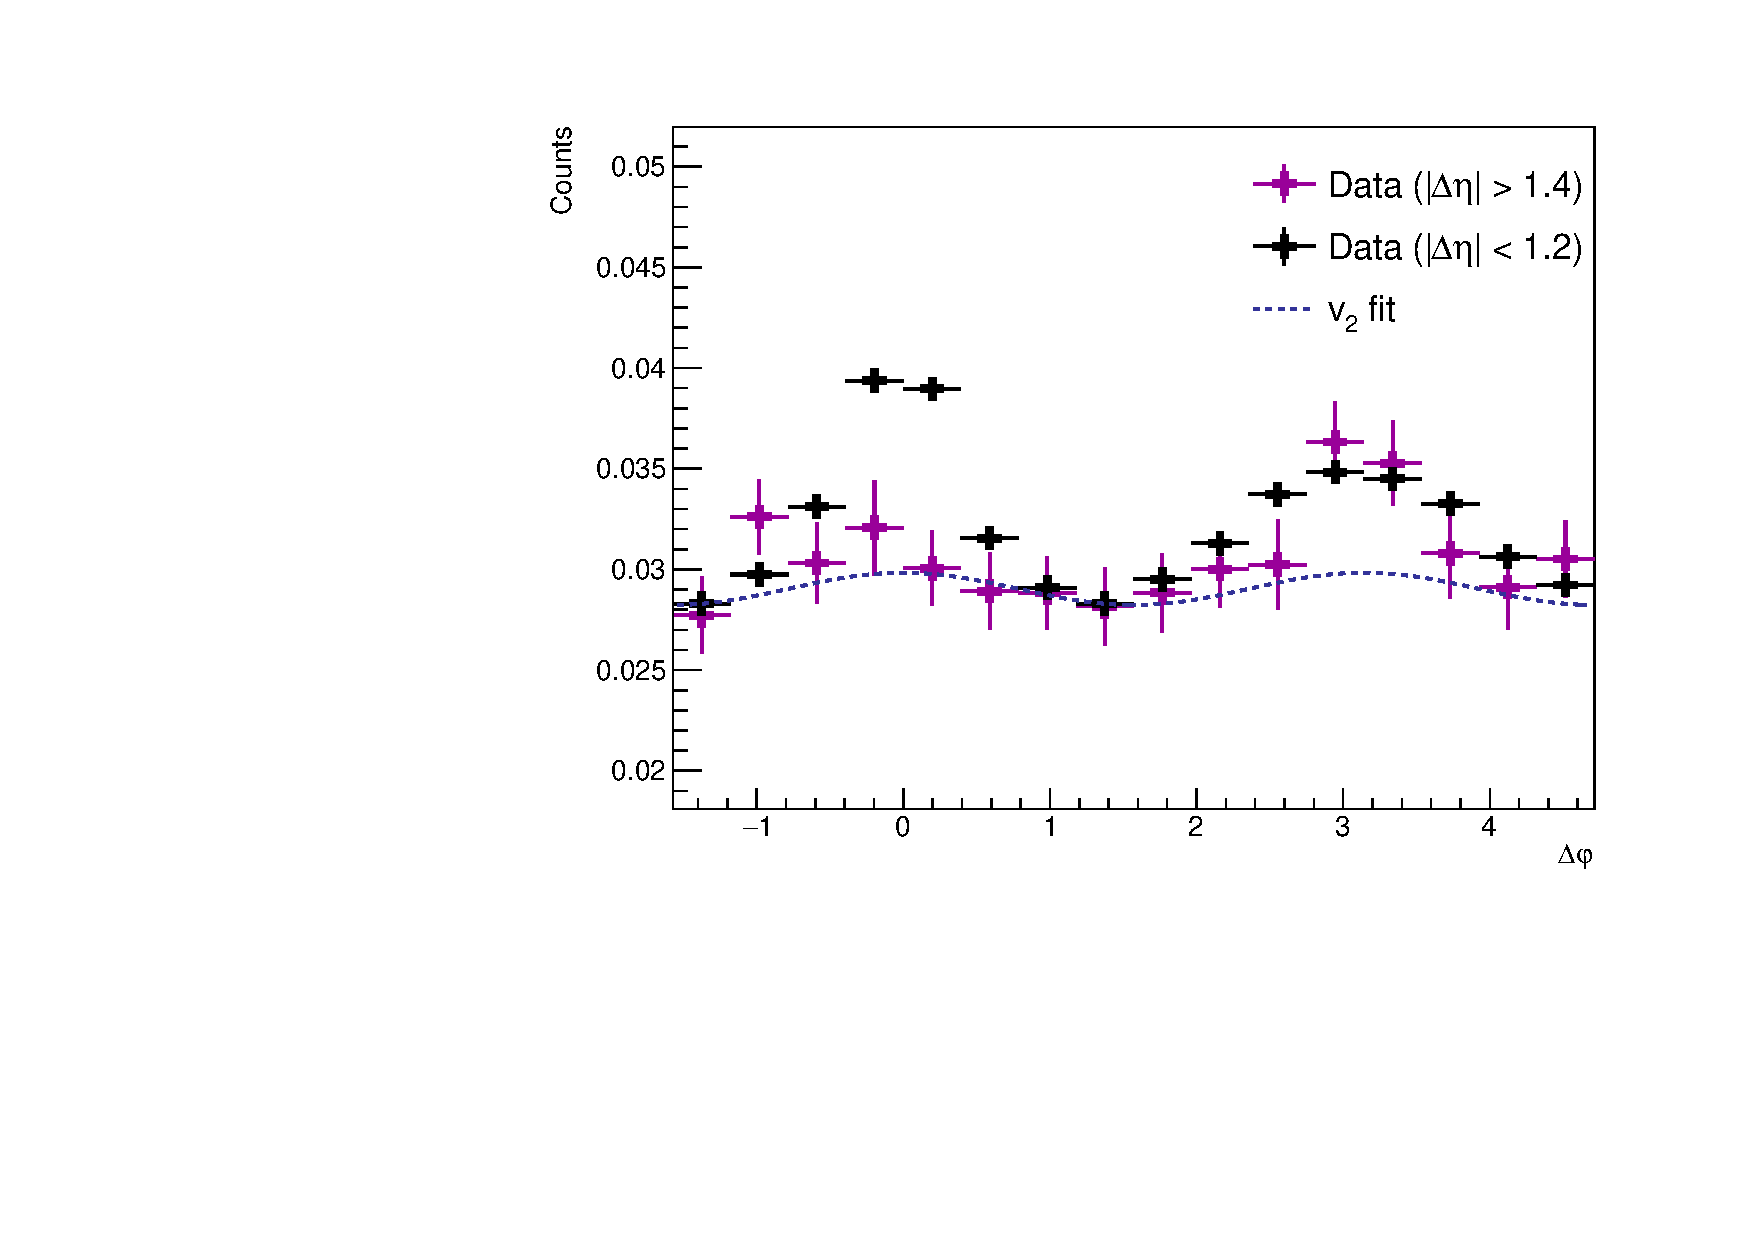
\includegraphics[width=0.49\textwidth]{figures/analysis/v2fit_largedeta_h_lambda_cent_0_20_trigger_4_8_assoc_25_4.pdf}
    \includegraphics[width=0.49\textwidth]{figures/analysis/v2fit_largedeta_h_h_cent_0_20_trigger_4_8_assoc_25_4.pdf}
    \caption{The h-\lmb (left) and h-h (right) $\Delta\varphi$ distributions in the 0-20\% multiplicity bin and higher \pt bin at small and large values of $\Delta\eta$, with the UE fit using the $v_{2}$-based procedure shown in blue. The fits are in good agreement with data in both cases.}
    \label{fig:v2_fit_large_deta}
\end{figure}

The effects of including $v_{2}$ on the extracted h-\lmb and h-h yields in each region is not obvious at first glance. For the most central collisions, the inclusion of $v_{2}$ results in nearly a 5\% decrease for the jet-like yields when compared to the nominal technique. This can mostly be seen in Figure~\ref{fig:v2_fit_examples}, where the peaks of the sinusoidal fit achieve their maxima within the near- and away-side components of the jet, causing the overall yields to be lower than those obtained by the flat UE assumption. However, at lower multiplicities (20-50\%, 50-80\%), the extracted h-\lmb and h-h jet-like yields actually exhibit a slight increase of around 5\% in their extracted yields when compared to those measured using the nominal UE fit. This is due to the variation of the pedestal $A$ in Equation~\ref{eq:ue_v2} during the fit, which results in a smaller pedestal value than the nominal fit in these multiplicity ranges. The extracted underlying event yield never deviates by more than 3\% from the yield obtained using the nominal procedure for all multiplicity and momentum bins for both the h-\lmb and h-h cases.

\subsubsection{Integration procedures}
\label{sec:integration_procedures}

The general yield-extraction equation
%
\begin{equation}
    \label{eq:general_yield}
    Y_{\Delta\varphi} = \int_{\Delta\varphi_1}^{\Delta\varphi_2} (\frac{dN}{d\Delta\varphi}- U(\Delta\varphi))d\Delta\varphi
\end{equation}
%
does not specify the integration procedure. Furthermore, there is nothing explicitly preventing 
%
\begin{equation}
    \frac{dN}{d\Delta\varphi} < U(\Delta\varphi),
\end{equation}
%
possibly resulting in a \textit{negative} yield, which is clearly unphysical. There are a few ways to alleviate these issues, which are discussed in this section.

For all of the yield extraction procedures discussed thus far, the usage of the integration symbol in Equation~\ref{eq:general_yield} is \textit{slightly} misleading: the yields are actually calculated by summing the bin contents of the $\Delta\varphi$ distribution in the specified range, and subtracting off the value of $U(\Delta\varphi)$ at the center of each bin. To be more explicit, the yields are calculated as
%
\begin{equation}
    \label{eq:yield_sum}
    Y_{\Delta\varphi} = \sum_{i=L}^{U} (\frac{dN}{d\Delta\varphi_{i}}- U(\Delta\varphi_{i})),
\end{equation}
%
where $L$ and $U$ are the bin numbers of the Lower and Upper $\Delta\varphi$ bins in the specified range, $dN/d\Delta\varphi_{i}$ is the value of the correlation distribution in the ith \dphi bin, and $U(\Delta\varphi)$ is the value of $U$ in the center of the ith \dphi bin. 

Equation~\ref{eq:yield_sum} provides an easy way to deal with the negative yield issue: if the value of $U(\Delta\varphi_{i})$ is greater than the value of $dN/d\Delta\varphi_{i}$ in a given bin, the yield in that bin is set to zero. While this is not done for the nominal yield extraction procedure in this analysis, it is a completely reasonable technique and is therefore explored in the systematic uncertainty analysis. Using the flat UE assumption with the UE average taken in the nominal range, the results are relatively unsurprising: the yields extracted using this procedure are strictly higher than those extracted using the main procedure where negative contributions are allowed. However, the deviations never exceed more than 3.5\%, with the average deviation being around 2\% for both the h-\lmb and h-h cases.

Another reasonable way to obtain the yields is by fitting these distributions with continuous functions, then use the corresponding fit for the integration in Equation~\ref{eq:general_yield}. This thesis considers two such functions, which are presented in the following two sections.

\subsubsection{The double Gaussian fit}
\label{sec:double_gaus_fit}

There are a number of functions that may appear suitable to fit the $\Delta\varphi$ distributions, but given the Gaussian-like appearance of the near- and away-side jet components, a double Gaussian fit is a natural choice. The double Gaussian fit function is given by
%
\begin{equation}
    \label{eq:double_gaus}
    \begin{split}
	&f(\Delta\varphi)  = U + A_{\text{NS}} e^{\frac{(\Delta\varphi - \mu_{\text{NS}})^2}{2\sigma_{\text{NS}}}} + A_{\text{AS}} e^{\frac{(\Delta\varphi - \mu_{\text{AS}})^2}{2\sigma_{\text{AS}}}} \\
    & + A_{\text{NS}}^{\text{mirror}} e^{\frac{(\Delta\varphi - \mu_{\text{NS}} + 2\pi)^2}{2\sigma_{\text{NS}}}} + A_{\text{AS}}^{\text{mirror}} e^{\frac{(\Delta\varphi - \mu_{\text{AS}} - 2\pi)^2}{2\sigma_{\text{AS}}}},
    \end{split}
\end{equation}
%
where $A$ and $\mu$ are the amplitude and means of the Gaussian components, and the subscript ``NS'' (``AS'') refers to the near-side (away-side) jet component. The ``mirror'' terms are added to account for the $2\pi$ periodicity of the $\Delta\varphi$ distribution, and are required to obtain a convergent fit. The $U$ term describes a flat underlying event, and is fixed to the average of the $\Delta\varphi$ distribution in the regions $[-\frac{\pi}{2}, -\frac{\pi}{4}) \cup [\frac{\pi}{4}, \frac{5\pi}{8}) \cup [\frac{11\pi}{8}, \frac{3\pi}{2})$, as is done for the nominal UE determination procedure. Furthermore, the mean in the near-side gaussian (and corresponding mirror term) is fixed to 0 ($2\pi$) and the mean in the away-side guassian (and corresponding mirror term) is fixed to $\pi$ ($-\pi$), leaving only the amplitudes and widths to vary freely. The double Gaussian fits to both the h-\lmb and h-h correlation distributions for every multiplicity and momentum bin are shown in Figures~\ref{fig:double_gaus_fits_lambda} (h-\lmb) and~\ref{fig:double_gaus_fits_h}. The fits generally describe the data quite well, though an extreme amount of effort went in to ensuring the convergence of each fit due to an inordinate amount of instability. 

The yields extracted using the double Gaussian fit are nearly identical to those extracted using the nominal bin-wise integration procedure, with deviations from the nominal procedure never exceeding 1\% for either the h-\lmb or h-h cases. This indicates two things:
%
\begin{enumerate}
    \item The fits describe the data quite well, and
    \item The differences between Equations~\ref{eq:general_yield} and~\ref{eq:yield_sum} are mostly aesthetic, so long as (1) holds and the choice of $U(\Delta\varphi)$ is consistent.
\end{enumerate}
%
As the deviations are so small, this procedure ends up excluded from the final systematic uncertainty calculation after the Barlow check in Section~\ref{sec:barlow_check_yield}, but the fits are still used for the systematic studies involving the near- and away-side jet widths discussed in Section~\ref{sec:systematics_width}.


\begin{figure}[ht]
    \centering
    \includegraphics[width=0.48\textwidth]{figures/analysis/h_lambda_dphi_gaus_0_20_lowpt.pdf}
    \includegraphics[width=0.48\textwidth]{figures/analysis/h_lambda_dphi_gaus_0_20_highpt.pdf}
    \includegraphics[width=0.48\textwidth]{figures/analysis/h_lambda_dphi_gaus_20_50_lowpt.pdf}
    \includegraphics[width=0.48\textwidth]{figures/analysis/h_lambda_dphi_gaus_20_50_highpt.pdf}
    \includegraphics[width=0.48\textwidth]{figures/analysis/h_lambda_dphi_gaus_50_80_lowpt.pdf}
    \includegraphics[width=0.48\textwidth]{figures/analysis/h_lambda_dphi_gaus_50_80_highpt.pdf}
    \caption{The final per-trigger h-\lmb $\Delta\varphi$ correlation distributions with the full double Gaussian fit for the 0-20\% (top), 20-50\%(middle), and 50-80\% (bottom) multiplicity bins in the lower (left) and higher (right) associated \pt bins. The UE fit is also shown as a dashed line.}
    \label{fig:double_gaus_fits_lambda}
\end{figure}
\begin{figure}[ht]
    \centering
    \includegraphics[width=0.48\textwidth]{figures/analysis/h_h_dphi_gaus_0_20_lowpt.pdf}
    \includegraphics[width=0.48\textwidth]{figures/analysis/h_h_dphi_gaus_0_20_highpt.pdf}
    \includegraphics[width=0.48\textwidth]{figures/analysis/h_h_dphi_gaus_20_50_lowpt.pdf}
    \includegraphics[width=0.48\textwidth]{figures/analysis/h_h_dphi_gaus_20_50_highpt.pdf}
    \includegraphics[width=0.48\textwidth]{figures/analysis/h_h_dphi_gaus_50_80_lowpt.pdf}
    \includegraphics[width=0.48\textwidth]{figures/analysis/h_h_dphi_gaus_50_80_highpt.pdf}
    \caption{The final per-trigger h-h $\Delta\varphi$ correlation distributions with the full double Gaussian fit for the 0-20\% (top), 20-50\%(middle), and 50-80\% (bottom) multiplicity bins in the lower (left) and higher (right) associated \pt bins. The UE fit is also shown as a dashed line.}
    \label{fig:double_gaus_fits_h}
\end{figure}

\clearpage

\subsubsection{The von Mises fit}
\label{sec:von_mises_fit}

While only briefly mentioned in Section~\ref{sec:yield_extraction} in the context of extracting the near- and away-side jet widths, the von Mises distribution is another natural choice for fitting the $\Delta\varphi$ distributions due to its combined Gaussian-like behaviour while naturally exhibiting $2\pi$-periodicity (which was ``forced'' onto the double Gaussian fit via the mirror terms). As a reminder, the von Mises fit function is given by
%
\begin{equation}
    \label{eq:von_mises}
    f(\Delta\varphi) = U(\Delta\varphi) + \frac{A_{\text{NS}}}{2\pi I_0(k_{\text{NS}})} e^{k_{\text{NS}}cos(\Delta\varphi - \mu_{\text{NS}})} + \frac{A_{\text{AS}}}{2\pi I_0(k_{\text{AS}})} e^{k_{\text{AS}}cos(\Delta\varphi - \mu_{\text{AS}})},
\end{equation}
%
where $A$ and $\mu$ are as they were in Equation~\ref{eq:double_gaus}, and $k$ is a measure of the collimation of the distribution, which is inversely related to the width through
%
\begin{equation}
    \label{eq:kappa_to_sigma}
    \sigma = \sqrt{-2\ln\frac{I_{1}(\kappa)}{I_{0}(\kappa)}}.
\end{equation}
%
In these equations, $I_n$ refers to the modified Bessel function of the nth kind. Note that the $U(\Delta\varphi)$ has been given explicit $\Delta\varphi$ dependence, as this fit function does not require the UE component to be flat with respect to $\Delta\varphi$ in order to converge nicely.

During the fitting procedure, the means $\mu_{\text{NS}}$ and $\mu_{\text{AS}}$ are again fixed to 0 and $\pi$, respectively, and the $U(\Delta\varphi)$ term is fixed to the function obtained by fitting the UE which includes a non-zero $v_{2}$ contribution, as described in Section~\ref{sec:ue_fit_v2}. While the fitting of this function is much more stable than the aforementioned double Gaussian function--possibly allowing for the variation of $U$ during the fit--the term is ultimately fixed due to an interesting feature of the von Mises distribution, which is discussed in~\ref{sec:systematics_width}. The von Mises fits to both the h-\lmb and h-h correlation distributions for every multiplicity and momentum bin are shown in Figures~\ref{fig:von_fits_lambda} (h-\lmb) and~\ref{fig:von_fits_h}. Again, the fits describe the data very well. Furthermore, the fits are extremely stable, which is a welcome change from the double Gaussian fits and was the initial motivation for the width analysis presented in this thesis.

Given these fits are taken with a different choice of $U(\Delta\varphi, \Delta\eta)$, the extracted yields from the von Mises function deviate from the nominal extraction procedure by a relatively large amount, with both the h-\lmb and h-h jet-like yields seeing a decrease of around 5\%. This percentage is familiarly the same as the percent deviation seen in Section~\ref{sec:ue_fit_v2} from the h-\lmb and h-h yields when using the $v_{2}$-based UE fit while still using bin-wise summation to extract the yields.  In fact, all of the yields extracted using the von Mises fitting procedure are nearly identical to the yields extracted using the $v_{2}$-based UE fit with bin-wise summation, again indicating that the data are well described by the fits. As these two procedures are nearly identical in their results, the von Mises fitting procedure is also excluded from the final systematic uncertainty calculation for the yield extraction after the Barlow check in Section~\ref{sec:barlow_check_yield}. However, the fits are so incredibly well-behaved that they spawned the initial investigation into the near- and away-side jet widths, which eventually became a major topic of interest in this thesis.\footnote{Systematic uncertainty calculations involving misbehaving fits are a nightmare.}

\begin{figure}[ht]
    \centering
    \includegraphics[width=0.48\textwidth]{figures/analysis/h_lambda_dphi_von_0_20_lowpt.pdf}
    \includegraphics[width=0.48\textwidth]{figures/analysis/h_lambda_dphi_von_0_20_highpt.pdf}
    \includegraphics[width=0.48\textwidth]{figures/analysis/h_lambda_dphi_von_20_50_lowpt.pdf}
    \includegraphics[width=0.48\textwidth]{figures/analysis/h_lambda_dphi_von_20_50_highpt.pdf}
    \includegraphics[width=0.48\textwidth]{figures/analysis/h_lambda_dphi_von_50_80_lowpt.pdf}
    \includegraphics[width=0.48\textwidth]{figures/analysis/h_lambda_dphi_von_50_80_highpt.pdf}
    \caption{The final per-trigger h-\lmb $\Delta\varphi$ correlation distributions with the von Mises fit for the 0-20\% (top), 20-50\% (middle), and 50-80\% (bottom) multiplicity bins in the lower (left) and higher (right) associated \pt bins. The UE fit with $v_{2}$ contribution is also shown as a dashed line.}
    \label{fig:von_fits_lambda}
\end{figure}

\begin{figure}[ht]
    \centering
    \includegraphics[width=0.48\textwidth]{figures/analysis/h_h_dphi_von_0_20_lowpt.pdf}
    \includegraphics[width=0.48\textwidth]{figures/analysis/h_h_dphi_von_0_20_highpt.pdf}
    \includegraphics[width=0.48\textwidth]{figures/analysis/h_h_dphi_von_20_50_lowpt.pdf}
    \includegraphics[width=0.48\textwidth]{figures/analysis/h_h_dphi_von_20_50_highpt.pdf}
    \includegraphics[width=0.48\textwidth]{figures/analysis/h_h_dphi_von_50_80_lowpt.pdf}
    \includegraphics[width=0.48\textwidth]{figures/analysis/h_h_dphi_von_50_80_highpt.pdf}
    \caption{The final per-trigger h-h $\Delta\varphi$ correlation distributions with the von Mises fit for the 0-20\% (top), 20-50\% (middle), and 50-80\% (bottom) multiplicity bins in the lower (left) and higher (right) associated \pt bins. The UE fit with $v_{2}$ contribution is also shown as a dashed line.}
    \label{fig:von_fits_h}
\end{figure}

\subsubsection{Barlow check for yield extraction}
\label{sec:barlow_check_yield}

Following the same procedure as outlined in Section~\ref{sec:barlow_check_dphi}, a Barlow check is performed for the different techniques for extracting the per-trigger yields from Equations~\ref{eq:jet_yields_ref} and~\ref{eq:ue_yield_ref}. If the majority of the measured h-$\Lambda$ yields for a given variation have $|N\sigma_{RB}| < 1$, that variation is excluded from the systematic uncertainty calculation. This majority is calculated across all kinematic regions (near-side jet, away-side jet, underlying event), multiplicity bins, and associated momentum bins. While the h-h yields were initially considered for this check, their statistical errors are so small that the denominator in Equation~\ref{eq:barlow_check} is close to zero, resulting in erratic $N\sigma_{RB}$ values. Thus, any technique which gets excluded for the h-$\Lambda$ yields will also be excluded for the h-h yields. Examples of the Barlow check for the yield extraction are shown in Figure~\ref{fig:barlow_check_yield_0_20}. 

As a result of the Barlow check, the following variations are excluded from the systematic uncertainty calculation:
%
\begin{itemize}
    \item The double Gaussian fit procedure
    \item The von Mises fit procedure
\end{itemize}
%
These exclusions were foreshadowed in the previous sections, as the fits describe the data well enough that there are no statistically significant differences between the yields extracted using these fit functions and the yields extracted using bin-wise summation.

\clearpage

\begin{figure}[ht]
    \centering
    \includegraphics[width=0.48\textwidth]{figures/analysis/h_lambda_yield_barlow_0_20_lowpt.pdf}
    \includegraphics[width=0.48\textwidth]{figures/analysis/h_lambda_yield_barlow_0_20_highpt.pdf}
    \caption{The Barlow check for the yield extraction procedure in the 0-20\% multiplicity bin for the lower (left) and higher (right) associated \pt bins. The red lines represent $N_{\sigma_{RB}} = \pm 1$, and if the majority of the points from a given procedure fall within these lines (across all multiplicity and momentum bins), the procedure is excluded from the systematic uncertainty calculation.}
    \label{fig:barlow_check_yield_0_20}
\end{figure}


\subsubsection{Yield extraction systematics, summarized}
\label{sec:yield_systematics_summary}
As most of the main results of this thesis involve the h-\lmb and h-h per-trigger yields in the various kinematic regions, the systematic uncertainties associated with the extraction of these yields deserve to be consolidated to concise tables and plots from the overly detailed descriptions of the previous sections. To that end, plots demonstrating the resulting yield deviations from the nominal technique for each of the aforementioned yield extraction procedure variations (post Barlow check) can be seen in Figures~\ref{fig:h_lambda_yield_deviations} (h-\lmb) and~\ref{fig:h_h_yield_deviations} (h-h). Furthermore, tables containing the final systematic uncertainties for both the h-\lmb and h-h per-trigger yields in each kinematic region for every multiplicity and associated \pt bin can be seen in Tables~\ref{tab:h_lambda_yield_systematics} (h-\lmb) and \ref{tab:h_h_yield_systematics} (h-h). Note that included in these systematic uncertainties are both the technique variations associated with the yield extraction procedure, as well as the variations in the yields due to the variations in the $\Delta\varphi$ distributions themselves (after the Barlow check), as discussed in Section~\ref{sec:systematics_dphi}. The UE yield systematic uncertainties are generally much lower than the jet-like yields, averaging around 3.5\% for both the h-\lmb and h-h cases. The larger uncertainties for the jet-like yields (4-7\%) are primarily due to the fact that the jet-like yield extraction techniques rely both on the integration procedure and the choice of $U(\Delta\varphi)$, where both including $v_{2}$ and excluding negative yield contributions can have a large effect on these extracted yields. Both of those choices have little effect (or no effect in the case of the non-negative yield requirement) on the integral of the $U(\Delta\varphi)$ across the entire azimuthal range (i.e. the UE yield). 

As was the case in Section~\ref{sec:dphi_systematics_summarized}, the portion of systematic uncertainty which is uncorrelated with multiplicity is computed using Equations~\ref{eq:uncorrelated_fraction_1} and~\ref{eq:uncorrelated_fraction_2} and presented in Tables~\ref{tab:h_lambda_mult_uncorrelated_yield_systematics} (h-\lmb) and~\ref{tab:h_h_mult_uncorrelated_yield_systematics}. Whenever the trends of these yields with respect to multiplicity are measured (either by taking slopes or looking at percent differences), the errors are always calculated using these multiplicity-uncorrelated systematic uncertainties.


\begin{figure}[ht]
    \centering
    \includegraphics[width=0.48\textwidth]{figures/analysis/h_lambda_0_20_lowpt_yield_variation.pdf}
    \includegraphics[width=0.48\textwidth]{figures/analysis/h_lambda_0_20_highpt_yield_variation.pdf}
    \includegraphics[width=0.48\textwidth]{figures/analysis/h_lambda_20_50_lowpt_yield_variation.pdf}
    \includegraphics[width=0.48\textwidth]{figures/analysis/h_lambda_20_50_highpt_yield_variation.pdf}
    \includegraphics[width=0.48\textwidth]{figures/analysis/h_lambda_50_80_lowpt_yield_variation.pdf}
    \includegraphics[width=0.48\textwidth]{figures/analysis/h_lambda_50_80_highpt_yield_variation.pdf}
    \caption{The deviation from the nominal h-\lmb per-trigger yields for each yield extraction procedure variation (post Barlow check) in each kinematic region for the 0-20\% (top), 20-50\% (middle), and 50-80\% (bottom) multiplicity bins in the lower (left) and higher (right) associated \pt bins. The systematic uncertainty for the yield extraction procedure is calculated by taking the RMS of these deviations for each kinematic region.}
    \label{fig:h_lambda_yield_deviations}
\end{figure}

\begin{figure}[ht]
    \centering
    \includegraphics[width=0.48\textwidth]{figures/analysis/h_h_0_20_lowpt_yield_variation.pdf}
    \includegraphics[width=0.48\textwidth]{figures/analysis/h_h_0_20_highpt_yield_variation.pdf}
    \includegraphics[width=0.48\textwidth]{figures/analysis/h_h_20_50_lowpt_yield_variation.pdf}
    \includegraphics[width=0.48\textwidth]{figures/analysis/h_h_20_50_highpt_yield_variation.pdf}
    \includegraphics[width=0.48\textwidth]{figures/analysis/h_h_50_80_lowpt_yield_variation.pdf}
    \includegraphics[width=0.48\textwidth]{figures/analysis/h_h_50_80_highpt_yield_variation.pdf}
    \caption{The deviation from the nominal h-h per-trigger yields for each yield extraction procedure variation (post Barlow check) in each kinematic region for the 0-20\% (top), 20-50\% (middle), and 50-80\% (bottom) multiplicity bins in the lower (left) and higher (right) associated \pt bins. The systematic uncertainty for the yield extraction procedure is calculated by taking the RMS of these deviations for each kinematic region.}
    \label{fig:h_h_yield_deviations}
\end{figure}

\begin{table}[h!]
    \centering
    \caption{Final systematic errors (in \%) for the per-trigger h-$\Lambda$ yields in each kinematic region, multiplicity, and momentum bin.}
    \label{tab:h_lambda_yield_systematics}
    \begin{tabular}{ l  c  c  c }
        \hline
        Mult. and \pt bin & Near-side (jet) & Away-side (jet) & UE  \\
        \hline
        0-20\%, low & 5.50e+00 & 5.57e+00 & 3.12e+00 \\
        20-50\%, low & 4.94e+00 & 5.24e+00 & 3.22e+00 \\
        50-80\%, low & 6.34e+00 & 7.19e+00 & 3.68e+00 \\
        0-20\%, high & 5.47e+00 & 6.10e+00  & 3.15e+00 \\
        20-50\%, high & 5.88e+00 & 6.54e+00  & 3.33e+00 \\
        50-80\%, high & 4.75e+00 & 5.25e+00  & 3.72e+00 \\
        \hline
    \end{tabular}
\end{table}

\begin{table}[h!]
    \centering
    \caption{Final systematic errors (in \%) for the h-h per-trigger yields in each kinematic region, multiplicity, and momentum bin.}
    \label{tab:h_h_yield_systematics}
    \begin{tabular}{ l  c  c  c }
        \hline
        Mult. and \pt bin & Near-side (jet) & Away-side (jet) & UE  \\
        \hline
        0-20\%, low & 4.46e+00   & 4.75e+00  & 3.51e+00 \\
        20-50\%, low & 3.75e+00 & 3.63e+00  & 3.50e+00 \\
        50-80\%, low & 4.94e+00 & 6.35e+00  & 3.67e+00 \\
        0-20\%, high & 3.80e+00   & 4.00e+00  & 3.51e+00 \\
        20-50\%, high & 3.61e+00 & 3.63e+00  & 3.51e+00 \\
        50-80\%, high & 4.17e+00 & 5.16e+00  & 3.81e+00 \\
        \hline
    \end{tabular}
\end{table}

\begin{table}[h!]
    \centering
    \caption{Final multiplicity-uncorrelated systematic errors (in \%) for the per-trigger h-$\Lambda$ yields in each kinematic region, multiplicity, and momentum bin, used for calculating errors associated with quantities describing trends versus multiplicity (slopes and percent changes).}
    \label{tab:h_lambda_mult_uncorrelated_yield_systematics}
    \begin{tabular}{ l  c  c  c }
        \hline
        Mult. and \pt bin & Near-side (jet) & Away-side (jet) & UE  \\
        \hline
        0-20\%, low & 2.73e+00 & 2.83e+00  & 6.66e-01 \\
        20-50\%, low & 3.09e+00 & 3.57e+00  & 1.00e+00 \\
        50-80\%, low & 5.80e+00 & 6.95e+00  & 2.23e+00 \\
        0-20\%, high & 2.91e+00 & 3.65e+00  & 7.40e-01 \\
        20-50\%, high & 4.32e+00 & 5.41e+00  & 1.28e+00 \\
        50-80\%, high & 4.47e+00 & 5.45e+00  & 2.35e+00 \\
        \hline
    \end{tabular}
\end{table}

\begin{table}[h!]
    \centering
    \caption{Final multiplicity-uncorrelated systematic errors (in \%) for the h-h per-trigger yields in each kinematic region, multiplicity and momentum bin, used for calculated errors associated with quantities describing trends versus multiplicity (slopes and percent changes).}
    \label{tab:h_h_mult_uncorrelated_yield_systematics}
    \begin{tabular}{ l  c  c  c }
        \hline
        Mult. and \pt bin & Near-side (jet) & Away-side (jet) & UE  \\
        \hline
        0-20\%, low & 1.72e+00   & 2.31e+00  & 1.86e-01 \\
        20-50\%, low & 1.31e+00 & 1.92e+00  & 2.29e-01 \\
        50-80\%, low & 3.95e+00 & 6.23e+00  & 1.21e+00 \\
        0-20\%, high & 1.03e+00   & 1.68e+00  & 2.42e-01 \\
        20-50\%, high & 7.24e-01 & 1.22e+00  & 2.76e-01 \\
        50-80\%, high & 2.28e+00 & 4.08e+00  & 1.54e+00 \\
        \hline
    \end{tabular}
\end{table}

\clearpage

\subsection{Near- and away-side width extraction}
\label{sec:systematics_width}

The extracted widths of the near- and away-side jet components from the \dphi distributions are also subject to a fair amount of systematic uncertainty, both from the variations of the \dphi distributions themselves as well as the techniques used to extract said widths. None of the $\Delta\varphi$ distributions variations are ``new,'' in that they have been discussed in some way within the previous sections. However, the effects of these variations on the extracted widths are not as straightforward as the effects on the yields, and thus deserve their own section. Furthermore, the fitting techniques used to extract the widths are different enough than the fitting techniques for yield extraction (Sections~\ref{sec:double_gaus_fit} and~\ref{sec:von_mises_fit}) that they should be discussed separately.

As a brief reminder, the nominal procedure for extracting the jet widths is by fitting the \dphi distribution to the von Mises-based fit function,
%
\begin{equation}
    \label{eq:von_mises_ref}
    f(\Delta\varphi) = U(\Delta\varphi) + \frac{A_{\text{NS}}}{2\pi I_0(k_{\text{NS}})} e^{k_{\text{NS}}cos(\Delta\varphi - \mu_{\text{NS}})} + \frac{A_{\text{AS}}}{2\pi I_0(k_{\text{AS}})} e^{k_{\text{AS}}cos(\Delta\varphi - \mu_{\text{AS}})},
\end{equation}
%
where $A$ and $\mu$ are the amplitudes and means of the von Mises components, and $k$ is a measure of the collimation of the distribution, which is inversely related to the width through
%
\begin{equation}
    \label{eq:kappa_to_sigma_ref}
    \sigma = \sqrt{-2\ln\frac{I_{1}(\kappa)}{I_{0}(\kappa)}}.
\end{equation}
%
In these equations, $I_n$ refers to the modified Bessel function of the nth kind. During the fitting procedure, the means $\mu_{\text{NS}}$ and $\mu_{\text{AS}}$ are again fixed to 0 and $\pi$, respectively, and the $U(\Delta\varphi)$ term is fixed to the function obtained by fitting the UE which includes a non-zero $v_{2}$ contribution, as described in Section~\ref{sec:ue_fit_v2}.

The reason for fixing the $U$ component during fitting is subtle, as the von Mises distributions describe the data extremely well and generally allow for the variation of this component while still obtaining a convergent fit. However, the form of the Von Mises function,
%
\begin{equation}
    \label{eq:von_mises_form}
    f(x) = e^{k cos(x)},
\end{equation}
%
 presents a unique issue: if the width is sufficiently large, meaning $k$ is sufficiently small ($\approx 1$), there is an ``offset'' from the $U$ term that never tapers off. This is fundamentally different from a Gaussian, which will always converge to zero (or $U$ in this case) at large enough $x$. A visual depiction of this effect can be seen in Figure~\ref{fig:von_mises_vs_gaus}. In most cases, this never presents an issue as the widths are usually such that $k > 2$. However, in the lowest momentum bin for the more central h-$\Lambda$ $\Delta\varphi$ distributions, allowing the $U$ term to vary during the fitting procedure has a very large effect on the corresponding $k$ value, as the fitting software tries to ``absorb'' this offset into $U$. Because of this, the $U$ term is fixed during all fitting procedures, and instead the techniques for determining $U$ are varied. 

\begin{figure}[ht]
    \centering
    \includegraphics[width=0.48\textwidth]{figures/analysis/von_plot.png}
    \includegraphics[width=0.48\textwidth]{figures/analysis/gaussian_plot.png}
    \caption{The Von Mises (left) and Gaussian (right) dist with $\kappa = 1$ and $\sigma = 1$. Note that the von Mises distribution does not approach zero at large x, while the Gaussian does.}
    \label{fig:von_mises_vs_gaus}
\end{figure}

\subsubsection{Signal, sideband, and PID cut variations}
\label{sec:cut_systematics_width}

Each of the signal, sideband, and PID cut variations that affect the $\Delta\varphi$ distributions (from Section~\ref{sec:systematics_dphi}) can also affect the corresponding extracted widths. To that end, the h-$\Lambda$ \dphi von Mises-based fits and extracted widths for each of these variations for all multiplicity and momentum bins can be seen in Figure~\ref{fig:cut_variations_widths}. Note that these widths were extracted using the nominal procedure described at the beginning of this section. Deviations from the nominal near-side widths never exceed 3.5\% in most cases, whereas the away-side width deviations are much larger, with some variations resulting in over a 10\% change from the nominal value, even after removing statistically insignificant variations via the Barlow procedure in Section~\ref{sec:barlow_check_width}. 

Again, problematic behavior arises from the PID cut variation, which requires a TOF hit for both of the $\Lambda$ daughters, with both the near- and away-side widths being particularly sensitive to this cut. As the lower momentum daughter pions are usually deflected by the detector's magnetic field before reaching the TOF, in cases when the pion actually generates a TOF signal, its corresponding momentum is likely higher than usual. This would result in a higher-than-usual $\Lambda$ momentum, which in turn would give lower-than-usual jet widths in the corresponding h-\lmb correlations as jets become less collimated as their constituent momentum decreases. To test this, the \pt distributions of $\Lambda$ candidates with and without the TOF signal are compared in Figure~\ref{fig:tof_momentum_bias}. The mean \pt of the $\Lambda$ candidates with daughters that generate a TOF signal is around 10\% higher than those without this requirement, which indicates that the TOF signal requirement introduces a physical bias into the h-$\Lambda$ \dphi distributions, manifesting as unusually low jet widths. Luckily, this requirement also happens to reduce the overall yield of $\Lambda$ candidates by a huge margin, causing a large amount of statistical fluctuations in the corresponding h-\lmb correlation distributions. Because of this, the TOF signal requirement ends up being excluded after the Barlow check. However, it is important to distinguish between excluding variations because they are statistically insignificant and excluding them because they introduce \textit{physical} biases into the data. Had the data sample been larger, the TOF signal requirement would have likely survived the Barlow check, leaving no choice but to rely on the aforementioned argument.

\begin{figure}[t]
    \centering
    \includegraphics[width=0.6\textwidth]{figures/analysis/quick_tof_pt_check.pdf}
    \caption{The \pt distributions of $\Lambda$ candidates with and without the TOF signal requirement. The mean \pt of the $\Lambda$ candidates with daughters that generate a TOF signal is nearly 10\% higher than those without this requirement, which indicates that the requiring a TOF signal for the \lmb daughters introduces a physical bias.}
    \label{fig:tof_momentum_bias}
\end{figure}

\begin{figure}[ht]
    \begin{minipage}{0.03\textwidth}
        \rotatebox{90}{\small{Signal region vars.}}
    \end{minipage}
    \hspace{-1.5cm}
    \begin{minipage}{1.1\textwidth}
        \centering
        \begin{tabular}{c c c}
            Low associated \pt & & High associated \pt \\
        \end{tabular}
        \begin{tabular}{c c ;{2pt/2pt} c c c}
            \includegraphics[width=0.17\textwidth]{figures/analysis/signal_variations_width_0_20_lowpt.pdf} &
            \includegraphics[width=0.17\textwidth]{figures/analysis/signal_variations_width_0_20_lowpt_widths.pdf} &
            \includegraphics[width=0.17\textwidth]{figures/analysis/signal_variations_width_0_20_highpt.pdf} &
            \includegraphics[width=0.17\textwidth]{figures/analysis/signal_variations_width_0_20_highpt_widths.pdf} & \rotatebox[origin=r]{-90}{\small{0-20\%}} \\ 
            \includegraphics[width=0.17\textwidth]{figures/analysis/signal_variations_width_20_50_lowpt.pdf} & 
            \includegraphics[width=0.17\textwidth]{figures/analysis/signal_variations_width_20_50_lowpt_widths.pdf} &
            \includegraphics[width=0.17\textwidth]{figures/analysis/signal_variations_width_20_50_highpt.pdf} &
            \includegraphics[width=0.17\textwidth]{figures/analysis/signal_variations_width_20_50_highpt_widths.pdf} & \rotatebox[origin=r]{-90}{\small{20-50\%}} \\
            \includegraphics[width=0.17\textwidth]{figures/analysis/signal_variations_width_50_80_lowpt.pdf} &
            \includegraphics[width=0.17\textwidth]{figures/analysis/signal_variations_width_50_80_lowpt_widths.pdf} &
            \includegraphics[width=0.17\textwidth]{figures/analysis/signal_variations_width_50_80_highpt.pdf} &
            \includegraphics[width=0.17\textwidth]{figures/analysis/signal_variations_width_50_80_highpt_widths.pdf} & \rotatebox[origin=r]{-90}{\small{50-80\%}} \\
            \hline
        \end{tabular}
    \end{minipage}
    \begin{minipage}{0.03\textwidth}
        \rotatebox{90}{\small{Sideband region vars.}}
    \end{minipage}
    \hspace{-1.5cm}
    \begin{minipage}{1.1\textwidth}
        \centering
        \begin{tabular}{c c ;{2pt/2pt} c c c}
            \includegraphics[width=0.17\textwidth]{figures/analysis/sideband_variations_width_0_20_lowpt.pdf} &
            \includegraphics[width=0.17\textwidth]{figures/analysis/sideband_variations_width_0_20_lowpt_widths.pdf} &
            \includegraphics[width=0.17\textwidth]{figures/analysis/sideband_variations_width_0_20_highpt.pdf} &
            \includegraphics[width=0.17\textwidth]{figures/analysis/sideband_variations_width_0_20_highpt_widths.pdf} & \rotatebox[origin=r]{-90}{\small{0-20\%}} \\ 
            \includegraphics[width=0.17\textwidth]{figures/analysis/sideband_variations_width_20_50_lowpt.pdf} & 
            \includegraphics[width=0.17\textwidth]{figures/analysis/sideband_variations_width_20_50_lowpt_widths.pdf} &
            \includegraphics[width=0.17\textwidth]{figures/analysis/sideband_variations_width_20_50_highpt.pdf} &
            \includegraphics[width=0.17\textwidth]{figures/analysis/sideband_variations_width_20_50_highpt_widths.pdf} & \rotatebox[origin=r]{-90}{\small{20-50\%}} \\
            \includegraphics[width=0.17\textwidth]{figures/analysis/sideband_variations_width_50_80_lowpt.pdf} &
            \includegraphics[width=0.17\textwidth]{figures/analysis/sideband_variations_width_50_80_lowpt_widths.pdf} &
            \includegraphics[width=0.17\textwidth]{figures/analysis/sideband_variations_width_50_80_highpt.pdf} &
            \includegraphics[width=0.17\textwidth]{figures/analysis/sideband_variations_width_50_80_highpt_widths.pdf} & \rotatebox[origin=r]{-90}{\small{50-80\%}} \\
            \hline
        \end{tabular}
    \end{minipage}
    \begin{minipage}{0.03\textwidth}
        \rotatebox{90}{\small{PID cut vars.}}
    \end{minipage}
    \hspace{-1.5cm}
    \begin{minipage}{1.1\textwidth}
        \centering
        \begin{tabular}{c c ;{2pt/2pt} c c c}
            \includegraphics[width=0.17\textwidth]{figures/analysis/pid_variations_width_0_20_lowpt.pdf} &
            \includegraphics[width=0.17\textwidth]{figures/analysis/pid_variations_width_0_20_lowpt_widths.pdf} &
            \includegraphics[width=0.17\textwidth]{figures/analysis/pid_variations_width_0_20_highpt.pdf} &
            \includegraphics[width=0.17\textwidth]{figures/analysis/pid_variations_width_0_20_highpt_widths.pdf} & \rotatebox[origin=r]{-90}{\small{0-20\%}} \\ 
            \includegraphics[width=0.17\textwidth]{figures/analysis/pid_variations_width_20_50_lowpt.pdf} & 
            \includegraphics[width=0.17\textwidth]{figures/analysis/pid_variations_width_20_50_lowpt_widths.pdf} &
            \includegraphics[width=0.17\textwidth]{figures/analysis/pid_variations_width_20_50_highpt.pdf} &
            \includegraphics[width=0.17\textwidth]{figures/analysis/pid_variations_width_20_50_highpt_widths.pdf} & \rotatebox[origin=r]{-90}{\small{20-50\%}} \\
            \includegraphics[width=0.17\textwidth]{figures/analysis/pid_variations_width_50_80_lowpt.pdf} &
            \includegraphics[width=0.17\textwidth]{figures/analysis/pid_variations_width_50_80_lowpt_widths.pdf} &
            \includegraphics[width=0.17\textwidth]{figures/analysis/pid_variations_width_50_80_highpt.pdf} &
            \includegraphics[width=0.17\textwidth]{figures/analysis/pid_variations_width_50_80_highpt_widths.pdf} & \rotatebox[origin=r]{-90}{\small{50-80\%}} \\
        \end{tabular}
    \end{minipage}
    \caption{The resulting von Mises fits and extracted jet widths after the signal, sideband and PID cut variations are applied to the h-$\Lambda$ $\Delta\varphi$ distributions.}
    \label{fig:cut_variations_widths}
\end{figure}

\subsubsection{Fitting procedure variations}
\label{sec:fitting_procedure_systematics_width}

Both of the fitting functions discussed in this thesis are of the form
%
\begin{equation}
    \label{eq:fit_function_form}
    f(\Delta\varphi) = U(\Delta\varphi) + f_{\text{NS}}(\Delta\varphi) + f_{\text{AS}}(\Delta\varphi),
\end{equation}
%
where $U$ is the underlying event function, and $f_{\text{NS}}$ ($f_{\text{AS}}$) is the distribution that describes the near-side (away-side) jet. To estimate the systematic uncertainty associated with the fitting procedure, the following variations are considered:
%
\begin{enumerate}
    \item \textbf{Varying $U(\Delta\varphi)$:} The $U(\Delta\varphi)$ term is varied by replacing the nominal $v_{2}$-based UE function with a flat line equal to the average of the $\Delta\varphi$ distribution in the ranges $[-\frac{\pi}{2}, -\frac{\pi}{4}) \cup [\frac{\pi}{4}, \frac{5\pi}{8}) \cup [\frac{11\pi}{8}, \frac{3\pi}{2})$ and $[-\frac{\pi}{2}, -\frac{3\pi}{8}) \cup [\frac{3\pi}{8}, \frac{5\pi}{8}) \cup [\frac{11\pi}{8}, \frac{3\pi}{2})$ (i.e. the nominal and restricted-range UE variations from the yield extraction procedure)
    \item \textbf{Varying the $f_{\text{NS}}$ and $f_{\text{AS}}$ functions:} The $f_{\text{NS}}$ and $f_{\text{AS}}$ functions are varied by replacing the nominal von Mises distributions with the Gaussian ones, as described in Section~\ref{sec:double_gaus_fit}, and the $U$ term is fixed to the average of the $\Delta\varphi$ distribution in the ranges $[-\frac{\pi}{2}, -\frac{\pi}{4}) \cup [\frac{\pi}{4}, \frac{5\pi}{8}) \cup [\frac{11\pi}{8}, \frac{3\pi}{2})$ (again, the nominal UE determination technique from the yield extraction procedure)
\end{enumerate}
%
More variations were initially considered--namely using the $v_{2}$-based UE with the Gaussian functions from Equation~\ref{eq:double_gaus} and trying generalized Gaussians~\cite{GeneralizedGaus} to describe the jet components--but they were discarded as many of the fits did not converge for all multiplicity and momentum ranges\footnote{This is a strict requirement, there are twelve fits in total, each with at least four free parameters, and the fitting software is not particularly robust.} despite a large amount of effort.


The choice of making the $v_{2}$-based UE determination procedure the nominal one was not made lightly, as it breaks the symmetry with the nominal yield extraction technique. In the presence of non-zero elliptic flow (as is likely the case at higher multiplicities), the $v_{2}$-based UE determination procedure is the most physically motivated, as it is the only one that takes into account the underlying event's azimuthal anisotropy. The only reason this procedure was not chosen as the nominal technique for yield extraction is extremely specific to this analysis: at the time of writing this thesis, the only available h-$\phi(1020)$ correlation results in \pPb at \snn = 5.02 \TeV come in the form of the h-$\phi$/h-h per-trigger yield ratios, where the yields are extracted assuming a flat UE. As mentioned in the abstract, one of the topics of this analysis involves investigating open versus hidden strangeness in the form of the h-\lmb/h-$\phi$ per-trigger yield ratios in the different kinematic regions. This is done by taking a ratio of ratios, namely
%
\begin{equation}
    \label{eq:ratio_of_ratios}
    \frac{(\text{h-}\Lambda)}{(\text{h-h})_{1}}/\frac{(\text{h-}\phi)}{(\text{h-h})_{2}}
\end{equation}
%
where the subscripts $1$ and $2$ are used to differentiate between this research and the $\phi$ analysis, respectively. This only reduces to the h-\lmb/h-$\phi$ ratios if two conditions are met: the first is that the h-h distributions are the same (which is investigated more thoroughly in Section ~\ref{sec:dihadron_comparison}), and the second is that the yields are extracted from these dihadron distributions using the exact same procedure. While this is not required in the case of the h-\lmb yields, the same procedure is applied for the sake of consistency. 


The resulting fits and extracted widths for each of the variations listed above in all multiplicity and momentum ranges for both the h-$\lmb$ and h-h cases can be seen in Figure~\ref{fig:fitting_procedure_variations}. Again, only small deviations from the central values are observed in the near-side widths across all variations, with the largest percent difference being around 3\% across all multiplicity and momentum bins for both the h-\lmb and h-h distributions. Interestingly, the away-side widths appear to be much more sensitive to the inclusion of $v_{2}$, as all variations from the nominal technique--again, each variation assumes a flat UE--result in widths which are systematically lower than the central values by around 5-10\%. This is a strange result, as the $v_{2}$-based UE is completely symmetric about $\Delta\varphi = \pi/2$, and thus should affect the near-side widths in the same way as the away-side. As mentioned above, including $v_{2}$ in the UE is the more \textit{physically} motivated choice, and therefore is chosen to be nominal despite these large deviations. Note that the Gaussian and von Mises widths are more similar in the cases where the flat UE is used, indicating that the observed deviations are not due to the choice of fitting function.

\begin{figure}[ht]
    \begin{minipage}{0.03\textwidth}
        \rotatebox{90}{\small{h-\lmb technique vars.}}
    \end{minipage}
    \hspace{-1.5cm}
    \begin{minipage}{1.1\textwidth}
        \centering
        \begin{tabular}{c c c}
            Low associated \pt & & High associated \pt \\
        \end{tabular}
        \begin{tabular}{c c ;{2pt/2pt} c c c}
            \includegraphics[width=0.17\textwidth]{figures/analysis/technique_variations_width_0_20_lowpt.pdf} &
            \includegraphics[width=0.17\textwidth]{figures/analysis/technique_variations_width_0_20_lowpt_widths.pdf} &
            \includegraphics[width=0.17\textwidth]{figures/analysis/technique_variations_width_0_20_highpt.pdf} &
            \includegraphics[width=0.17\textwidth]{figures/analysis/technique_variations_width_0_20_highpt_widths.pdf} & \rotatebox[origin=r]{-90}{\small{0-20\%}} \\ 
            \includegraphics[width=0.17\textwidth]{figures/analysis/technique_variations_width_20_50_lowpt.pdf} & 
            \includegraphics[width=0.17\textwidth]{figures/analysis/technique_variations_width_20_50_lowpt_widths.pdf} &
            \includegraphics[width=0.17\textwidth]{figures/analysis/technique_variations_width_20_50_highpt.pdf} &
            \includegraphics[width=0.17\textwidth]{figures/analysis/technique_variations_width_20_50_highpt_widths.pdf} & \rotatebox[origin=r]{-90}{\small{20-50\%}} \\
            \includegraphics[width=0.17\textwidth]{figures/analysis/technique_variations_width_50_80_lowpt.pdf} &
            \includegraphics[width=0.17\textwidth]{figures/analysis/technique_variations_width_50_80_lowpt_widths.pdf} &
            \includegraphics[width=0.17\textwidth]{figures/analysis/technique_variations_width_50_80_highpt.pdf} &
            \includegraphics[width=0.17\textwidth]{figures/analysis/technique_variations_width_50_80_highpt_widths.pdf} & \rotatebox[origin=r]{-90}{\small{50-80\%}} \\
            \hline
        \end{tabular}
    \end{minipage}
    \begin{minipage}{0.03\textwidth}
        \rotatebox{90}{\small{h-h technique vars.}}
    \end{minipage}
    \hspace{-1.5cm}
    \begin{minipage}{1.1\textwidth}
        \centering
        \begin{tabular}{c c ;{2pt/2pt} c c c}
            \includegraphics[width=0.17\textwidth]{figures/analysis/hh_technique_variations_width_0_20_lowpt.pdf} &
            \includegraphics[width=0.17\textwidth]{figures/analysis/hh_technique_variations_width_0_20_lowpt_widths.pdf} &
            \includegraphics[width=0.17\textwidth]{figures/analysis/hh_technique_variations_width_0_20_highpt.pdf} &
            \includegraphics[width=0.17\textwidth]{figures/analysis/hh_technique_variations_width_0_20_highpt_widths.pdf} & \rotatebox[origin=r]{-90}{\small{0-20\%}} \\ 
            \includegraphics[width=0.17\textwidth]{figures/analysis/hh_technique_variations_width_20_50_lowpt.pdf} & 
            \includegraphics[width=0.17\textwidth]{figures/analysis/hh_technique_variations_width_20_50_lowpt_widths.pdf} &
            \includegraphics[width=0.17\textwidth]{figures/analysis/hh_technique_variations_width_20_50_highpt.pdf} &
            \includegraphics[width=0.17\textwidth]{figures/analysis/hh_technique_variations_width_20_50_highpt_widths.pdf} & \rotatebox[origin=r]{-90}{\small{20-50\%}} \\
            \includegraphics[width=0.17\textwidth]{figures/analysis/hh_technique_variations_width_50_80_lowpt.pdf} &
            \includegraphics[width=0.17\textwidth]{figures/analysis/hh_technique_variations_width_50_80_lowpt_widths.pdf} &
            \includegraphics[width=0.17\textwidth]{figures/analysis/hh_technique_variations_width_50_80_highpt.pdf} &
            \includegraphics[width=0.17\textwidth]{figures/analysis/hh_technique_variations_width_50_80_highpt_widths.pdf} & \rotatebox[origin=r]{-90}{\small{50-80\%}} \\
        \end{tabular}
    \end{minipage}
    \caption{The resulting h-\lmb (top) and h-h (bottom) von Mises fits and extracted jet widths in each multiplicity and momentum bin after each variation of the fitting procedure.}
    \label{fig:fitting_procedure_variations}
\end{figure}

\clearpage

\subsubsection{Barlow check for width extraction}
\label{sec:barlow_check_width}

Again, following the same techniques as outlined in Sections~\ref{sec:barlow_check_dphi} and~\ref{sec:barlow_check_yield}, a Barlow check is performed for the variations presented in this section that affect the extracted near- and away-side widths. As was before, if the majority of the extracted h-$\Lambda$ widths for a given variation have $|N\sigma_{RB}| < 1$, that variation is excluded from the systematic uncertainty calculation. This majority is calculated using both the near- and away-side jet components across all multiplicity bins and associated momentum bins. Again, the dihadron widths are not considered for this procedure\footnote{Due to extremely small statistical errors, see Section~\ref{sec:barlow_check_yield}}, and any fitting technique variation that is excluded from the uncertainty calculation as the result of this check for the h-$\Lambda$ widths will also be excluded for the h-h case. Visual depictions of the Barlow procedure can be seen in Figure~\ref{fig:barlow_check_width_20_50}.

As a result of the check, the following variations were excluded from the systematic uncertainty calculation for the jet widths:
%
\begin{itemize}
    \item Signal: Wide, Wider
    \item Sideband: Wide, Narrow
    \item PID: Require TOF
\end{itemize}
%
Curiously, these are the same variations that were excluded for the $\Delta\varphi$ distributions, which is \textit{mostly}\footnote{There is obviously some correlation between variations in the individual $\Delta\varphi$ bins and the widths. Consider a hypothetical variation that causes an unusually large spike in a $\Delta\varphi$ bin near zero: this would certainly cause the near-side width to be considerably smaller than normal. This is an extreme example, however, and generally these variations affect the individual $\Delta\varphi$ bins in similar ways.} a coincidence. 

\begin{figure}[ht]
    \centering
    \includegraphics[width=0.32\textwidth]{figures/analysis/width_signal_barlow_20_50.pdf}
    \includegraphics[width=0.32\textwidth]{figures/analysis/width_sideband_barlow_20_50.pdf}
    \includegraphics[width=0.32\textwidth]{figures/analysis/width_pid_barlow_20_50.pdf}
    \caption{Barlow check for the width extraction procedure for the signal (left), sideband (middle), and PID (right) variations in the 20-50\% multiplicity bin. The red lines represent $N\sigma_{RB} = \pm 1$, and if the majority of the points fall within the red lines (across all \pt and multiplicity bins), they are excluded from the width systematic uncertainty calculation.}
    \label{fig:barlow_check_width_20_50}
\end{figure}

\subsubsection{Width extraction systematics, summarized}
\label{sec:width_systematics_summary}

The systematic uncertainties associated with the h-\lmb and h-h jet width extraction for each multiplicity and associated momentum bin can be seen in Tables~\ref{tab:h_lambda_width_systematics} (h-\lmb) and~\ref{tab:h_h_width_systematics} (h-h), with visual depictions shown in Figures~\ref{fig:h_lambda_width_systematics_plots} (h-\lmb) and~\ref{fig:h_h_width_systematics_plots}. The total systematic uncertainties are obtained by adding the individual uncertainties in quadrature. Note that the away-side width uncertainties are much larger than the near-side, indicating that constraining the away-side jet width is a much more difficult procedure, especially in the presence of non-zero elliptic flow (as discussed in Section~\ref{sec:fitting_procedure_systematics_width}). As the width uncertainties do not exhibit any significant multiplicity dependence, the multiplicity-uncorrelated portion of these uncertainties is not reported.

Both the topological selection and associated hadron efficiency uncertainties are given in the tables and figures, which were obtained by randomly varying the $\Delta\varphi$ distributions within their respective systematic uncertainties (Table~\ref{tab:flat_systematics}) and extracting the widths using the nominal procedure. As the topological selection and tracking efficiency uncertainties were not directly calculated in this analysis, these results serve as a ``best guess'' for how the widths would be affected by variations in the corresponding selection criteria. The results of this procedure for the h-\lmb and h-h distributions in the 20-50\% multiplicity bin for both associated momentum ranges can be seen in Figure~\ref{fig:topo_eff_widths}. 



\begin{table}[ht]
    \centering
    \begin{tabular}{| c c c | c c c c c | c |}
        \hline
        Mult. & \pt & Peak & Signal & Sideband & PID & Fit proc. & Topo. & Total \\
        \hline

        0-20\% & low & NS & 1.19 & 5.41 & 1.19 & 2.09 & 3.40 & 6.93 \\
        20-50\% & low & NS & 1.13 & 2.70 & 1.74 & 0.93 & 3.40 & 4.90 \\
        50-80\% & low & NS & 3.20 & 1.19 & 3.82 & 2.05 & 3.40 & 6.48 \\
        0-20\% & low & AS & 2.53 & 1.64 & 6.21 & 7.91 & 2.40 & 10.77 \\
        20-50\% & low & AS & 0.57 & 4.68 & 2.62 & 8.16 & 2.40 & 10.07 \\
        50-80\% & low & AS & 2.88 & 9.43 & 4.11 & 5.88 & 2.40 & 12.43 \\
        \hline
        0-20\% & high & NS & 3.44 & 1.66 & 2.19 & 3.51 & 3.10 & 6.43 \\
        20-50\% & high & NS & 1.10 & 0.48 & 1.09 & 1.35 & 3.10 & 3.75 \\
        50-80\% & high & NS & 2.46 & 0.56 & 1.68 & 1.54 & 3.10 & 4.60 \\
        0-20\% & high & AS & 0.51 & 1.00 & 1.99 & 8.95 & 6.10 & 11.07 \\
        20-50\% & high & AS & 1.56 & 1.93 & 5.02 & 10.33 & 6.10 & 13.24 \\
        50-80\% & high & AS & 3.93 & 5.74 & 10.80 & 5.40 & 6.10 & 15.21 \\
        \hline

    \end{tabular}
    \caption{The final systematic errors from the h-$\Lambda$ $\Delta\varphi$ near-side (NS) and away-side (AS) width extraction for each multiplicity bin in the lower (top) and higher (bottom) associated \pt bins. The total systematic error is calculated by adding each systematic error in quadrature.}
    \label{tab:h_lambda_width_systematics}
\end{table}

\begin{table}[ht]
    \centering
    \begin{tabular}{| c c c | c c | c |}
        \hline
        Mult. & \pt & Peak & Fit proc. & Trk. eff. & Total \\
        \hline
        0-20\% & low & NS & 2.21 & 1.00 & 2.42 \\
        20-50\% & low & NS & 0.21 & 1.00 & 1.02 \\
        50-80\% & low & NS & 1.74 & 1.00 & 2.01 \\
        0-20\% & low & AS & 8.75 & 1.50 & 8.87 \\
        20-50\% & low & AS & 6.66 & 1.50 & 6.82 \\
        50-80\% & low & AS & 6.91 & 1.50 & 7.07 \\
        \hline
        0-20\% & high & NS & 1.86 & 1.00 & 2.11 \\
        20-50\% & high & NS & 0.12 & 1.00 & 1.01 \\
        50-80\% & high & NS & 1.47 & 1.00 & 1.78 \\
        0-20\% & high & AS & 8.02 & 1.50 & 8.16 \\
        20-50\% & high & AS & 6.06 & 1.50 & 6.24 \\
        50-80\% & high & AS & 5.73 & 1.50 & 5.93 \\
        \hline
    \end{tabular}
    \caption{The final systematic errors from the h-h $\Delta\varphi$ near-side (NS) and away-side (AS) width extraction for each multiplicity bin in the lower (top) and higher (bottom) associated \pt bins. The total systematic error is calculated by adding each systematic error in quadrature.}
    \label{tab:h_h_width_systematics}
\end{table}


\begin{figure}[ht]
    \centering
        \includegraphics[width=0.48\textwidth]{figures/analysis/systematics_ns_width_postbarlow_lowpt.pdf}
        \includegraphics[width=0.48\textwidth]{figures/analysis/systematics_ns_width_postbarlow_highpt.pdf}
        \includegraphics[width=0.48\textwidth]{figures/analysis/systematics_as_width_postbarlow_lowpt.pdf}
        \includegraphics[width=0.48\textwidth]{figures/analysis/systematics_as_width_postbarlow_highpt.pdf}
    \caption{Final systematic errors for the h-$\Lambda$ $\Delta\varphi$ near-side (top) and away-side (bottom) width extraction for each multiplicity bin in the lower (left) and higher (right) associated \pt bins.}
    \label{fig:h_lambda_width_systematics_plots}
\end{figure}

\begin{figure}[ht]
    \centering
        \includegraphics[width=0.48\textwidth]{figures/analysis/systematics_ns_hh_width_postbarlow_lowpt.pdf}
        \includegraphics[width=0.48\textwidth]{figures/analysis/systematics_ns_hh_width_postbarlow_highpt.pdf}
        \includegraphics[width=0.48\textwidth]{figures/analysis/systematics_as_hh_width_postbarlow_lowpt.pdf}
        \includegraphics[width=0.48\textwidth]{figures/analysis/systematics_as_hh_width_postbarlow_highpt.pdf}
    \caption{Final systematic errors for the h-h $\Delta\varphi$ near-side (top) and away-side (bottom) width extraction for each multiplicity bin in the lower (left) and higher (right) associated \pt bins.}
    \label{fig:h_h_width_systematics_plots}
\end{figure}

\begin{figure}[ht]
    \begin{minipage}{0.03\textwidth}
        \rotatebox{90}{\small{h-\lmb}}
    \end{minipage}
    \hspace{-1.5cm}
    \begin{minipage}{1.1\textwidth}
        \centering
        \begin{tabular}{c c c}
            Low associated \pt & & High associated \pt \\
        \end{tabular}
        \begin{tabular}{c c ;{2pt/2pt} c c}
            \includegraphics[width=0.17\textwidth]{figures/analysis/h_lambda_cent_20_50_trigger_4_8_assoc_15_25_topo_variations.pdf} & 
            \includegraphics[width=0.17\textwidth]{figures/analysis/h_lambda_cent_20_50_trigger_4_8_assoc_15_25_topo_variations_widths.pdf} &
            \includegraphics[width=0.17\textwidth]{figures/analysis/h_lambda_cent_20_50_trigger_4_8_assoc_25_4_topo_variations.pdf} &
            \includegraphics[width=0.17\textwidth]{figures/analysis/h_lambda_cent_20_50_trigger_4_8_assoc_25_4_topo_variations_widths.pdf} \\
            \hline
        \end{tabular}
    \end{minipage}
    \begin{minipage}{0.03\textwidth}
        \rotatebox{90}{\small{h-h}}
    \end{minipage}
    \hspace{-1.5cm}
    \begin{minipage}{1.1\textwidth}
        \centering
        \begin{tabular}{c c ;{2pt/2pt} c c}
            \includegraphics[width=0.17\textwidth]{figures/analysis/h_h_cent_20_50_trigger_4_8_assoc_15_25_topo_variations.pdf} & 
            \includegraphics[width=0.17\textwidth]{figures/analysis/h_h_cent_20_50_trigger_4_8_assoc_15_25_topo_variations_widths.pdf} &
            \includegraphics[width=0.17\textwidth]{figures/analysis/h_h_cent_20_50_trigger_4_8_assoc_25_4_topo_variations.pdf} &
            \includegraphics[width=0.17\textwidth]{figures/analysis/h_h_cent_20_50_trigger_4_8_assoc_25_4_topo_variations_widths.pdf} \\
        \end{tabular}
    \end{minipage}
    \caption{The resulting h-\lmb (top) and h-h (bottom) von Mises fits and extracted jet widths in the 20-50\% multiplicity bin for each momentum bin after random variations of the individual $\Delta\varphi$ bins within the topological selection (h-\lmb) and tracking efficiency (h-h) uncertainties from Table~\ref{tab:flat_systematics}.}
    \label{fig:topo_eff_widths}
\end{figure}

\clearpage

\subsection{Final systematics tables}
\label{ref:final_systematics_tables}

For ease of reference, all of the final systematic uncertainties discussed in the previous sections have been consolidated into Tables~\ref{tab:h_lambda_final_systematics} (h-\lmb) and~\ref{tab:h_h_final_systematics} (h-h).

\begin{table}[h]
    \centering
    \caption{The final systematic uncertainties for the h-$\Lambda$ $\Delta\varphi$ distributions, the per-trigger jet and UE yields, and the jet widths in all multiplicity and associated momentum bins. The fraction of the systematic uncertainty which is uncorrelated with multiplicity is reported separately in parentheses for the extracted yields. The low (high) momentum bin is such that $1.5 < p_{T}^{\text{assoc.}} < 2.5$ \GeVc ($2.5 < p_{T}^{\text{assoc.}} < 4.0$ \GeVc).}
    \label{tab:h_lambda_final_systematics}
    \begin{tabular}{| c | c c c c c c |}
        \hline
        Mult. and \pt bin & $\Delta\varphi$ dist. & $Y_{near}$ & $Y_{away}$ & $Y_{UE}$ & $\sigma_{NS}$ & $\sigma_{away}$ \\
        \hline
        0-20\%, low & 3.3\% & 5.5(2.7)\% & 5.6(2.8)\% & 3.1(0.7)\% & 6.9\% & 10.8\% \\
        20-50\%, low & 3.4\% & 4.9(3.1)\% & 5.2(3.6)\% & 3.2(1.0)\% & 4.9\% & 10.1\% \\
        50-80\%, low & 3.8\% & 6.3(5.8)\% & 7.2(7.0)\% & 3.7(2.2)\% & 6.5\% & 12.4\% \\
        \hline
        0-20\%, high & 3.2\% & 5.5(2.9)\% & 6.1(3.7)\% & 3.2(0.7)\% & 6.4\% & 11.1\% \\
        20-50\%, high & 3.3\% & 5.9(4.3)\% & 6.5(5.4)\% & 3.3(1.3)\% & 3.8\% & 13.2\% \\
        50-80\%, high & 4.1\% & 4.8(4.5)\% & 5.3(5.5)\% & 3.7(2.4)\% & 4.6\% & 15.2\% \\
        \hline
    \end{tabular}
\end{table}

\begin{table}[h]
    \centering
    \caption{The final systematic uncertainties for the h-h $\Delta\varphi$ distributions, the per-trigger jet and UE yields, and the jet widths in all multiplicity and associated momentum bins. The fraction of the systematic uncertainty which is uncorrelated with multiplicity is reported separately in parentheses for the extracted yields. The low (high) momentum bin is such that $1.5 < p_{T}^{\text{assoc.}} < 2.5$ \GeVc ($2.5 < p_{T}^{\text{assoc.}} < 4.0$ \GeVc).}
    \label{tab:h_h_final_systematics}
    \begin{tabular}{| c | c c c c c c |}
        \hline
        Mult. and \pt bin & $\Delta\varphi$ dist. & $Y_{near}$ & $Y_{away}$ & $Y_{UE}$ & $\sigma_{NS}$ & $\sigma_{away}$ \\
        \hline
        0-20\%, low & 3.5\% & 4.5(1.7)\% & 4.8(2.3)\% & 3.5(0.2)\% & 2.4\% & 8.9\% \\
        20-50\%, low & 3.5\% & 3.8(1.3)\% & 3.6(1.9)\% & 3.5(0.2)\% & 1.0\% & 6.8\% \\
        50-80\%, low & 3.5\% & 4.9(3.9)\% & 6.4(6.2)\% & 3.7(1.2)\% & 2.0\% & 7.1\% \\
        \hline
        0-20\%, high & 3.5\% & 3.8(1.0)\% & 4.0(1.7)\% & 3.5(0.2)\% & 2.1\% & 8.2\% \\
        20-50\%, high & 3.5\% & 3.6(0.7)\% & 3.6(1.2)\% & 3.5(0.3)\% & 1.0\% & 6.2\% \\
        50-80\%, high & 3.5\% & 4.2(2.3)\% & 5.2(4.1)\% & 3.8(1.5)\% & 1.8\% & 5.9\% \\
        \hline
    \end{tabular}
\end{table}


\clearpage

\section{Cross-checks}
\label{sec:cross_checks}

As mentioned in the introduction to this chapter, this section presents a number of cross-checks that were performed to verify the validity and robustness of the analysis procedure.

\subsection{Monte Carlo closure tests}
\label{sec:mc_closure_tests}

One of the most common procedures for verifying the validity of an experimental analysis comes in the form of a \textbf{Monte Carlo closure test}~\cite{MCClosure}. The basic steps of any MC closure test are as follows:
%
\begin{enumerate}
    \item Generate a large sample of simulated events using a Monte Carlo generator, which models both the physics of the collision and the detector response
    \item Apply the same analysis method and selection criteria to the detector-simulated events as to the experimental data to obtain a \textbf{reconstructed} observable
    \item Compare the reconstructed observable with the \textbf{ground-truth} observable, which is obtained directly from the generator-level particles
\end{enumerate}
%
Generally the third step is done by taking a ratio of the reconstructed observable to the ground-truth observable, which should be consistent with unity if the analysis procedure is valid. Significant deviations from unity would indicate that the experimental procedure introduces a non-physical bias to the measurement, which should be addressed.  

For the Monte Carlo closure tests presented in this section, the \pPb collision events are simulated using the DPMJet generator~\cite{DPMJet}, with the ALICE detector response to the simulated particles handled by the GEANT~\cite{GEANT} software package. The reconstructed h-$\Lambda$ and h-h 2D correlation distributions are generated using the same procedure as described in~\ref{ch:analysis_details}. In particular, this means that:
%
\begin{itemize}
    \item Both the reconstructed trigger and associated \lmb (h) pass the track cuts described in Tables~\ref{tab:trigger_track_cuts} and \ref{tab:lambda_selection} (\ref{tab:primary_track_cuts}), respectively 
    \item To avoid issues with PID using GEANT\footnote{The $n\sigma_{\text{TPC},\text{TOF}}$ values predicted by GEANT differ from experimental data by a large margin, so using GEANT for PID is generally avoided whenever possible.}, the $\Lambda$ daughter tracks are verified to be from a proton/pion by checking their corresponding generator-level particles
    \item The efficiency and acceptance corrections are applied to the h-h and h-\lmb distributions in the same was as described in Section \ref{sec:corrections}
    \item The additional corrections (sideband subtraction, signal scaling, and two-track template) are applied to the h-\lmb distributions as they are in Section \ref{sec:lambda_corrections}
\end{itemize}
%
For the ground-truth distributions, the trigger and associated \lmb (h) are taken directly from the generator-level particles. The same kinematic cuts are also applied, namely the trigger is required to have momentum $4.0 <$ \pt $< 8.0$ \GeVc, the associated \lmb (h) have the same momentum ranges as the reconstructed case, and all particles are required to fall within $|\eta| < 0.8$. Applying these pseudorapidity cuts on the trigger and associated particles ensures that the underlying physics\footnote{Particle production is rapidity-dependent, so choosing particles in a different rapidity range could alter the spectrum.} is the same as the reconstructed case. Unfortunately this requirement also introduces the same triangular shape along $\Delta\eta$ in the correlation distributions as seen in data, which is corrected for using the mixed-event technique described in Section~\ref{sec:corrections}.

Both the reconstructed and ground-truth 2D correlation distributions are projected onto $\Delta\varphi$ in the range $|\Delta\eta| < 1.2$, and the results for the h-\lmb and h-h $\Delta\varphi$ distributions are shown for each associated \pt bin in Figures~\ref{fig:h_lambda_closure} (h-\lmb) and~\ref{fig:h_h_closure} (h-h), along with the corresponding (reconstructed)/(ground-truth) distribution ratios. A fit to the ratio is also shown, which is consistent with unity in all cases. This indicates that the analysis procedure is valid, and that the corrections applied to the h-\lmb and h-h distributions are not introducing any non-physical biases to the $\Delta\varphi$ distribution measurements. As all of the observables are derived directly from these distributions, it is safe to assume the reconstructed and ground-truth versions of these observables are also consistent with each other.

While the MC closure tests provide a general framework for checking the validity of an experimental analysis, there are a few more specific checks that are performed to ensure the robustness of this analysis, which are described in the following sections.

\begin{figure}[ht]
    \centering
    \includegraphics[width=0.49\textwidth]{figures/analysis/h_lambda_dphi_closure_lowpt.pdf}
    \includegraphics[width=0.49\textwidth]{figures/analysis/h_lambda_dphi_closure_ratio_lowpt.pdf}
    \includegraphics[width=0.49\textwidth]{figures/analysis/h_lambda_dphi_closure_highpt.pdf}
    \includegraphics[width=0.49\textwidth]{figures/analysis/h_lambda_dphi_closure_ratio_highpt.pdf}
    \caption{The reconstructed (pink) and ground-truth (blue) h-$\Lambda$ $\Delta\varphi$ distributions in the lower (top) and higher (bottom) associated \pt bins, along with a (reconstructed)/(ground-truth) ratio and straight-line fit with errors shown as dashed lines. The ratio is consistent with unity, and thus the corrections applied to the h-$\Lambda$ distributions are valid.}
    \label{fig:h_lambda_closure}
\end{figure}

\begin{figure}[ht]
    \centering
    \includegraphics[width=0.49\textwidth]{figures/analysis/h_h_dphi_closure_lowpt.pdf}
    \includegraphics[width=0.49\textwidth]{figures/analysis/h_h_dphi_closure_ratio_lowpt.pdf}
    \includegraphics[width=0.49\textwidth]{figures/analysis/h_h_dphi_closure_highpt.pdf}
    \includegraphics[width=0.49\textwidth]{figures/analysis/h_h_dphi_closure_ratio_highpt.pdf}
    \caption{The reconstructed (pink) and ground-truth (blue) h-h $\Delta\varphi$ distributions in the lower (top) and higher (bottom) associated \pt bins, along with a (reconstructed)/(ground-truth) ratio and straight-line fit with errors shown as dashed lines. Again, the ratio is consistent with unity, and thus the corrections applied to the h-h distributions are valid.}
    \label{fig:h_h_closure}
\end{figure}

\clearpage

\subsection{Investigating radial flow effects}
\label{sec:radial_flow}

Any multiplicity-differential analysis involving a sample of particles within a fixed \pt momentum window will be subject to \textbf{radial flow} effects. Radial (or directed) flow~\cite{DirectedFlow2} can be characterized by the increase of the average transverse momentum \meanpt with increasing event multiplicity for a given particle species. This could result in an increased yield integrated within a fixed \pt window, and that increase may be different for different particle species. As this thesis presents many results concerning the \lmb/h($\pi$) ratio as a function of multiplicity within fixed \pt ranges, it is important to investigate the effect radial flow may have on the final results.

Luckily, the effects of radial flow have \textit{already} been thoroughly investigated for the $\phi(1020)$/$\pi$ ratio, where it was found that radial flow causes a larger increase in the $\pi$ yield than the $\phi$ yield within the $2 <$ \pt $< 4$ \GeVc momentum window. This would result in a \textit{decrease} in the $\phi / \pi$ ratio with increasing multiplicity. Thus, any observation of an \textit{increase} in the $\phi/\pi$ ratio with increasing multiplicity can not be attributed to radial flow effects. Importantly, the \lmb baryon shares a similar mass (1.115 vs. 1.020 \GeVmass) and \pt spectrum shape (shown in Figure~\ref{fig:phi_lambda_pt}) to the $\phi$ meson. As such, any conclusion regarding the radial flow effects (which are determined using these two observables) on the \lmb/$\pi$ results can be inferred from the $\phi/\pi$ study. A brief summary of the $\phi/\pi$ radial flow study is presented below.


\begin{figure}
    \centering
    \includegraphics[width=0.9\textwidth]{figures/analysis/lambda_phi_pt_comp.png}
    \caption{The \pt spectra shape of the $\phi$ (triangles) and $\Lambda$ (squares) in p--Pb collisions at $\sqrt{s_{\text{NN}}} = 5.02$ TeV in the 0-5\% (red) and 60-80\% (green) multiplicity bins. Both spectra in the 0-5\% have been normalized to unity, whereas the 60-80\% spectra has been normalized to 0.5 for visibility. The \lmb and $\phi$ spectra shapes are very similar in both multiplicity bins.}
    \label{fig:phi_lambda_pt}
\end{figure}

\subsubsection{Radial flow effects on the $\phi$/$\pi$ ratio}

First, the mean \pt of both the $\phi$ and $\pi$ were taken from published p--Pb data in the 0-5\% and 60-80\% multiplicity percentiles. Then, the momentum spectra of the $\phi$ and $\pi$ were fit to the simplified Boltzman function,
%
\begin{equation}
    \label{eq:boltz_eq}
    B\left(p_{\mathrm{T}}\right)=\frac{C}{T(m+T)} p_{\mathrm{T}}e^{-\left(m_{\mathrm{T}}-m\right) / T },
\end{equation}
where $m$ is the particle mass, $m_{\text{T}}$ is the particle's transverse mass ($= \sqrt{p_{\mathrm{T}}^{2}+m^{2}}$), $T$ is the temperature, and $C$ is a normalization constant. The temperature $T$ was found such that the mean \pt of the fit function matched the published mean \pt values. The resulting fits are shown for the $\phi$ and the $\pi$ in both multiplicity bins in Figure~\ref{fig:phi_pi_radial_flow}. The $2 <$ \pt $< 4$ \GeVc momentum window is also highlighted.

\begin{figure}[ht]
    \centering
    \includegraphics[width=\textwidth]{figures/analysis/phi_pi_radial_flow.png}
    \caption{The fits to the momentum spectra of the $\phi$ (left) and $\pi$ (right) in the 0-5\% (red) and 60-80\% (green) multiplicity bins, with fit function given by Equation~\ref{eq:boltz_eq}. The $2 <$ \pt $< 4$ \GeVc momentum window is highlighted in blue.}
    \label{fig:phi_pi_radial_flow}
\end{figure}

The ratio of the yields in the higher multiplicity bin to the lower multiplicity bin within the momentum window was then calculated for both the $\phi$ and the $\pi$, which revealed that the $\phi$ yield increases by around 30\%, whereas the $\pi$ yield increases by nearly 200\%.



\subsection{Correlations with a single trigger}
\label{sec:single_trigger_correlations}

A central feature of this analysis relies on the assumption that the per-trigger pair-wise yields from the h-\lmb or h-h distributions are roughly equal to the per-trigger associated yields for \lmb baryons or charged hadrons in events that have a trigger hadron, so that the (h-\lmb)/(h-h) yield results can be interpreted as the \lmb/h ratio in each region. This is only true if there is only a single trigger hadron in each event, which is obviously not the case across a large event sample. To see why this is required, consider two events: the first has a single trigger with three associated particles, while the second has two triggers with three associated particles. In the first event, there are three trigger-associated pairs, which corresponds exactly to the number of associated particles in the event. In the second, there are twice as many pairs as there are associated particles, meaning that the pair-wise yield ``double counts'' the associated particles. A diagram of this effect is shown in Figure~\ref{fig:pairwise_counting}. This effect scales with the number of triggers: if there are $N$ triggers in an event, there would be $N$ times as many pairs as associated particles. This diagram also introduces another subtle effect of multiple triggers: if triggers $t_1$ and $t_2$ belong to separate jets within a single event, then the associated particles that fall into the jet-like regions when correlated with $t_1$ could be mistakenly placed in the ``underlying event'' when correlated with $t_2$, artificially inflating the UE yields.

\begin{figure}[ht]
    \centering
    \includegraphics[width=0.7\textwidth]{figures/analysis/pair_counting_diagram.png}
    \caption{A diagram showing the effect of multiple triggers on the per-trigger pair-wise yield. In the first event, there is a single trigger with three associated particles, so the pair-wise yield is equal to the number of associated particles. In the second event, there are two triggers with three associated particles, so the pair-wise yield is twice the number of associated particles.}
    \label{fig:pairwise_counting}
\end{figure}

Luckily, less than 1\% of all events have more than a single trigger, as shown in Figure~\ref{fig:trigs_per_event}. Even still, the effect of multiple triggers on the per-trigger pair-wise yield is investigated by repeating the same analysis procedure as described in the previous chapter, with one change:
%
\begin{itemize}
    \item If an event has more than one trigger, only the trigger with the highest momentum within the $4.0 <$ \pt $< 8.0$ \GeVc range is used
\end{itemize}
%
This guarantees that no associated particles will be counted more than once, at the expense of a slightly modified trigger \pt spectrum\footnote{Selecting the highest \pt trigger in the 4-8 \GeVc range usually still amounts to selecting a $\approx 4$ \GeVc particle.}. The final single trigger h-\lmb and h-h $\Delta\varphi$ distributions for each multiplicity bin are compared with the original method (all trigger) distributions in Figure~\ref{fig:single_trigger_comp}. A flat deviation of around 5\% is observed for both the h-\lmb and h-h cases, which is consistent across all multiplicity bins.

\begin{figure}[ht!]
    \centering
    \includegraphics[width=0.8\textwidth]{figures/analysis/trig_per_event.pdf}
    \caption{A log-plot showing the number of triggers per event across the entire data sample. Only a small fraction of events have at least a single trigger, and of those events, only a small fraction have more than one trigger.}
    \label{fig:trigs_per_event}
\end{figure}

As the (single trigger)/(all trigger) distribution ratios are mostly flat for both the h-\lmb and h-h distributions across all multiplicity bins, the effect on the final yield measurements would only be a $\approx 5\%$ change of scale along the y-axis, and the ratio measurements would remain unchanged. Furthermore, this scale factor is the same across all multiplicity bins, indicating that using the standard per-trigger correlation method accurately captures the multiplicity-dependent behavior of the \lmb/h ratios in events with a trigger. Because the conclusions drawn from the results of this thesis only rely on the relative y-axis behavior of the measured observables, the effect of multiple triggers on the final distributions is negligible.


\begin{figure}[ht]
    \centering
    \includegraphics[width=0.32\textwidth]{figures/analysis/h_lambda_dphi_subtracted_0_20_singletrigger.pdf}
    \includegraphics[width=0.32\textwidth]{figures/analysis/h_lambda_dphi_subtracted_20_50_singletrigger.pdf}
    \includegraphics[width=0.32\textwidth]{figures/analysis/h_lambda_dphi_subtracted_50_80_singletrigger.pdf}
    \includegraphics[width=0.32\textwidth]{figures/analysis/h_h_dphi_0_20_singletrigger.pdf}
    \includegraphics[width=0.32\textwidth]{figures/analysis/h_h_dphi_20_50_singletrigger.pdf}
    \includegraphics[width=0.32\textwidth]{figures/analysis/h_h_dphi_50_80_singletrigger.pdf}
    \includegraphics[width=0.32\textwidth]{figures/analysis/singletrigger_ratio_0_20.pdf}
    \includegraphics[width=0.32\textwidth]{figures/analysis/singletrigger_ratio_20_50.pdf}
    \includegraphics[width=0.32\textwidth]{figures/analysis/singletrigger_ratio_50_80.pdf}
    \caption{The per-trigger h-$\Lambda$ (top) and h-h (middle) $\Delta\varphi$ distribution comparison between using a single trigger (closed points) and all triggers (open points) in a given event, along with the (single trigger)/(all trigger) distribution ratio (bottom), for the 0-20\% (left), 20-50\% (center), and 50-80\% (bottom) multiplicity bins in the associated momentum range $2.0 <$ \pt $< 4.0$ \GeVc. The distributions are nearly identical up to a $\approx 0.95$ scale factor, which is constant as a function of multiplicity.}
    \label{fig:single_trigger_comp}
\end{figure}

\clearpage

\subsection{Dihadron comparison with $\phi$ analysis}
\label{sec:dihadron_comparison}

As mentioned in Section~\ref{sec:fitting_procedure_systematics_width}, the differences between open and hidden strangeness are investigated by taking the \lmb/$\phi(1020)$ per-trigger yield ratios in the different kinematic regions (e.g. near-side jet, away-side jet, and underlying event). This is done by taking a ratio of ratios, namely
%
\begin{equation}
    \label{eq:ratio_of_ratios_2}
    \frac{(\text{h-}\Lambda)}{(\text{h-h})_{1}}/\frac{(\text{h-}\phi)}{(\text{h-h})_{2}},
\end{equation}
%
where the (h-$\phi$)/(h-h)$_2$ ratio in the denominator is taken from previously published results in \pPb collisions at \snn = 5.02 \TeV which use the same angular correlation techniques to extract the per-trigger yields in the different regions~\cite{JustinPaper}. This only reduces to the per-trigger (h-\lmb)/(h-$\phi$) $\approx$ \lmb/$\phi$ yield ratios if two conditions are met:
%
\begin{enumerate}
    \item The (h-h)$_1$ and (h-h)$_2$ yields are identical
    \item The yields are extracted using the same procedure
\end{enumerate}
% 
Condition 2 has been met by design, as both analyses assume a flat UE taken as the average of the correlation distributions in the same \dphi regions, and they both use bin-wise summation to extract the per-trigger yields. Condition 1, however, needs to be checked more thoroughly. While all of the selection criteria is the same between the two, the analyses were performed by two different humans with vastly different coding styles.

To this end, a direct comparison between the dihadron per-trigger \dphi distributions from this analysis and the $\phi$ analysis is shown in Figure~\ref{fig:dihadron_comp}. The distributions are nearly identical across all multiplicity bins, which is indicated by the ratios at the bottom of the figure never deviating unity. As such, the cancellation of the (h-h)$_1$ and (h-h)$_2$ yields in Equation~\ref{eq:ratio_of_ratios_2} is valid.

\begin{figure}[ht]
    \includegraphics[width=0.32\textwidth]{figures/analysis/h_h_dphi_0_20_justin_ryan_comparison.pdf}
    \includegraphics[width=0.32\textwidth]{figures/analysis/h_h_dphi_20_50_justin_ryan_comparison.pdf}
    \includegraphics[width=0.32\textwidth]{figures/analysis/h_h_dphi_50_80_justin_ryan_comparison.pdf}
    \includegraphics[width=0.32\textwidth]{figures/analysis/justin_ryan_ratio_0_20}
    \includegraphics[width=0.32\textwidth]{figures/analysis/justin_ryan_ratio_20_50}
    \includegraphics[width=0.32\textwidth]{figures/analysis/justin_ryan_ratio_50_80}
    \caption{Comparison of the the dihadron $\Delta\varphi$ correlations between the $\phi$ and $\Lambda$ analyses for the 0-20\% (left), 20-50\% (middle), and 50-80\% (right) multiplicity bins, taken in the $2.0 <$ \pt $< 4.0$ \GeVc associated momentum range. They are functionally identical for all multiplicity bins.}
    \label{fig:dihadron_comp}
\end{figure}

\subsection{Resonance technique for \lmb reconstruction}
\label{sec:resonance_technique}

The \lmb baryons used in this analysis are reconstructed by exploiting their characteristic V$^0$ decay topology, as discussed in Section~\ref{sec:lambda_reconstruction}. However, this method introduces a small physical bias in the \lmb sample: only $\Lambda$s which decay far enough from the primary vertex to be reconstructed as V$^0$s (i.e. they have a detector-resolvable secondary vertex) are considered. While the average decay length of the \lmb is quite large (c$\tau \approx 7.89$ cm where $\tau$ is the average lifetime), decay length distributions are exponentials of the form $e^{-t/\tau}$. This means that there is a small fraction of $\Lambda$s that decay too quickly to be resolved using their V$^0$ topology, and thus are not included in the analysis. While the single particle \lmb efficiency is used to correct for the overall \lmb yield, it may be possible that the h-\lmb correlation shape is influenced by the exclusion of these short-lived \lmb baryons. 

To investigate this possible bias, a new set of h-\lmb distributions are produced, where the associated $\Lambda$s are reconstructed using the \textbf{resonance technique}: all oppositely charged proton-pion pairs from the event are combined to form \lmb candidates. This is the only way to reconstruct extremely short-lived particles--like resonances--as they will never have a resolvable secondary vertex.  This technique gives access to all \lmb baryons that \textit{can} be reconstructed in the event, regardless of their decay length. However, the large combinatorial background associated with the resonance technique presents many difficulties, which are discussed thoroughly in Appendix~\ref{ap:resonance}. Even still, it is possible to repeat the same analysis procedure from the previous chapter with $\Lambda$s reconstructed using this technique, and the resulting h-\lmb $\Delta\varphi$ distributions are shown in Figure~\ref{fig:resonance_v0_dphi_comp}, along with the original distributions for comparison. It should be noted that neither of the distributions are corrected for the two-track inefficiency or the branching ratio, as this investigation was performed prior to those tools being developed in this analysis. However, the comparison should be mostly\footnote{The two-track inefficiency is actually very slightly less for the resonance technique as the shorter-lived $\Lambda$s usually have daughter tracks with higher quality track parameters due to more hits in the detector, making them less likely to be merged with the trigger.} unaffected by these corrections, as they are the same in both cases.

The distributions are very similar across all multiplicity bins, although the resonance technique distributions exhibit much larger statistical fluctuations due to the subtraction of the large combinatorial background using the sideband procedure. This provides solid evidence that the V$^0$ reconstruction technique is not introducing a significant bias in the shape of the h-\lmb $\Delta\varphi$ distributions, and that the exclusion of short-lived \lmb baryons has little effect on the final results.

\begin{figure}[h!]
    \centering
    \includegraphics[width=0.32\textwidth]{figures/analysis/h_lambda_dphi_0_20_zeroed_rescomp.pdf}
    \includegraphics[width=0.32\textwidth]{figures/analysis/h_lambda_dphi_20_50_zeroed_rescomp.pdf}
    \includegraphics[width=0.32\textwidth]{figures/analysis/h_lambda_dphi_50_80_zeroed_rescomp.pdf}
    \caption{The final per-trigger h-$\Lambda$ $\Delta\varphi$ correlations for $\Lambda$s reconstructed using the resonance technique (blue) and the V$^{0}$-based technique (red) in the 0-20\% (left), 20-50\% (middle), and 50-80\% (right) multiplicity bins, taken in the associated momentum range $2.0 <$ \pt $< 4.0$ \GeVc, after the subtraction of the UE. The distributions show good agreement across all multiplicity bins, indicating that the V$^{0}$-based reconstruction technique is not introducing a bias in the correlation shape.}
    \label{fig:resonance_v0_dphi_comp}
\end{figure}

After calculating the systematic uncertainties and performing the various cross-checks described in this chapter, the final results of this thesis are ready to be presented.